% !TEX program = xelatex
%==============================================================================
% 2026 年 MathorCup 数学应用挑战赛——大数据竞赛 论文模板（LaTeX 版）
%------------------------------------------------------------------------------
% 首页版式对照官方 Word 模板逐项复刻（坐标经 PDF 实测校准）：
%   A4；上下 2.0cm、左右 2.5cm（1134 / 1418 缇）；行网格 15.6 磅（312 缇）
%   队伍编号/赛道表格：0.5 磅全框线、居中、行高 22.7 / 23.6 磅
%   浅灰分隔线：ECECEC / 1.5 磅 / 长 411.3 磅 / 左偏 2.65 磅
%   论文题目 14pt（顶部 159.9pt）→ 摘　要 12pt（184.4pt）→ 摘要正文（200.0pt）
%   → 关键词（465.2pt，即正文与关键词之间空 16 行网格）
%
% 一、二、三级标题沿用本机数模模板规范（templates/zh/mathorcup-latex）：
%   一级：居中 黑体加粗 14pt，编号“一、”，段前 1.25em 段后 1.05em
%   二级：左对齐 黑体加粗 12pt，编号“1.1”，段前 0.9em 段后 0.55em
%   三级：左对齐 黑体加粗 12pt，编号“1.1.1”，段前 0.65em 段后 0.4em
%   正文：宋体 12pt / 行距 15.6pt / 首行缩进 2em / 两端对齐
% 每章独立成文件，置于 sections/ 下，由 main.tex 逐个 \input。
%
% 编译：xelatex main.tex（跑两遍，生成目录与“共 Y 页”）
%==============================================================================
\documentclass[12pt, a4paper, fontset=none]{ctexart}

%---------- 页面：与 Word 完全一致 ----------
\usepackage[a4paper,
  left=70.9pt, right=70.9pt,      % 2.5cm（1418 缇）
  top=56.7pt, bottom=56.7pt,      % 2.0cm（1134 缇）
  headheight=13.6pt, headsep=0pt,
  footskip=4.8pt]{geometry}

%---------- 字体：正文宋体 + Calibri；标题黑体；题目/摘要/页脚 Times New Roman ----------
\usepackage{fontspec}
\usepackage{xeCJK}
\setmainfont{Calibri}                                    % Word 文档默认西文字体
\setsansfont{Arial}
\setmonofont{Courier New}
\setCJKmainfont[AutoFakeBold=2.5]{SimSun}                % 宋体
\setCJKfamilyfont{zhhei}[AutoFakeBold=2.5]{SimHei}       % 黑体
\newcommand{\heiti}{\CJKfamily{zhhei}}
\newfontfamily\tnrfont{Times New Roman}
% Word 不做行首标点悬挂；quanjiao 样式会让行首的（）等符号外溢到版心外
\xeCJKsetup{PunctStyle=plain}

%---------- 正文：12pt / 行距 15.6pt（= Word 文档网格 312 缇）----------
\renewcommand{\normalsize}{\fontsize{12pt}{15.6pt}\selectfont}
\renewcommand{\small}{\fontsize{10.5pt}{15.6pt}\selectfont}
\linespread{1}
\setlength{\parindent}{2em}
\setlength{\parskip}{0pt}
\widowpenalty=0 \clubpenalty=0
% 中文段落里拉丁词/数字串无法断开时，允许最后一遍额外拉伸，避免 overfull hbox
\setlength{\emergencystretch}{1.5em}
% 图表与正文之间的垂直间距收紧，控制正文页数
\setlength{\textfloatsep}{8pt plus 2pt minus 2pt}
\setlength{\floatsep}{8pt plus 2pt minus 2pt}
\setlength{\intextsep}{8pt plus 2pt minus 2pt}
\setlength{\abovecaptionskip}{4pt}
\setlength{\belowcaptionskip}{2pt}
%---------- 浮动体参数：避免图把整页占满而正文被推到下一页 ----------
% topfraction 放宽到 0.9，允许页顶放两张图；textfraction 降到 0.07，
% 要求每页至少留约两行正文位置；floatpagefraction 提高，减少纯图页。
\renewcommand{\topfraction}{0.9}
\renewcommand{\bottomfraction}{0.7}
\renewcommand{\textfraction}{0.07}
\renewcommand{\floatpagefraction}{0.78}
\setcounter{topnumber}{3}
\setcounter{bottomnumber}{2}
\setcounter{totalnumber}{4}


%---------- 数学与图表 ----------
\usepackage{amsmath, amssymb}
\usepackage{graphicx}
\usepackage{pdflscape}
\usepackage{array}
\usepackage{booktabs}
\usepackage{caption}
\usepackage{subcaption}   % 支持并排子图（相关图成对排列，单图放大配文字）
\usepackage{float}
\usepackage[section]{placeins}   % 图表只在本节内浮动，不越过 \section 漂到下一章
\usepackage{longtable}
\usepackage{listings}
\renewcommand{\figurename}{图}
\renewcommand{\tablename}{表}
% 按竞赛 AI 工具使用规定第 6 条，插图处注明 AI 贡献：绘图代码由 AI 辅助编写，
% 图中数据与结论经队员核验。用自定义 caption 格式统一附加，避免逐图改写。
\DeclareCaptionFormat{aifig}{#1#2#3\hspace{0.5em}\textnormal{\footnotesize AI 辅助绘制，数据经队员核验}}
\captionsetup{font={small}, labelsep=quad, justification=centering, singlelinecheck=true}
\captionsetup[figure]{format=aifig}
% 子图注只写简短标签，不带 AI 声明（AI 声明只在总图注出现一次）
\captionsetup[subfigure]{format=default, labelsep=quad, justification=centering}
\lstset{
  basicstyle=\ttfamily\fontsize{9pt}{11.7pt}\selectfont,
  breaklines=true,
  breakatwhitespace=false,
  columns=fullflexible,
  frame=single,
  numbers=left,
  numberstyle=\fontsize{8pt}{9.6pt}\selectfont,
  showstringspaces=false,
}

%---------- 标题编号：一、 / 1.1 / 1.1.1 ----------
\ctexset{
  section/number       = \chinese{section},
  subsection/number    = \arabic{section}.\arabic{subsection},
  subsubsection/number = \arabic{section}.\arabic{subsection}.\arabic{subsubsection},
}

%---------- 标题格式（titlesec） ----------
\usepackage{titlesec}
\titleformat{\section}
  {\centering\fontsize{14pt}{16.8pt}\heiti\bfseries}
  {\chinese{section}、}{1em}{}
\titleformat{\subsection}
  {\fontsize{12pt}{14.4pt}\heiti\bfseries}
  {\arabic{section}.\arabic{subsection}}{1em}{}
\titleformat{\subsubsection}
  {\fontsize{12pt}{14.4pt}\heiti\bfseries}
  {\arabic{section}.\arabic{subsection}.\arabic{subsubsection}}{1em}{}
\titlespacing{\section}       {0pt}{1.25em}{1.05em}
\titlespacing{\subsection}    {0pt}{0.9em}{0.55em}
\titlespacing{\subsubsection} {0pt}{0.65em}{0.4em}

%---------- 目录：收录到三级标题，点线引导 ----------
% 对应 Word 的 toc1/toc2/toc3 样式：
%   一级 12pt 加粗，编号“一、”与标题连排，缩进 0
%   二级 11pt 加粗，编号“1.1”，缩进 10.5 磅（210 缇）
%   三级 11pt 常规，编号“1.1.1”，缩进 21 磅（420 缇）
\setcounter{tocdepth}{2}
\usepackage{tocloft}
% tocloft 加载完再设一次：目录只到二级，三级标题不上目录
\setcounter{tocdepth}{2}
\renewcommand{\cftsecfont}{\fontsize{12pt}{14.2pt}\bfseries}
\renewcommand{\cftsecpagefont}{\bfseries}
\renewcommand{\cftsubsecfont}{\fontsize{11pt}{13.4pt}\bfseries}
\renewcommand{\cftsubsecpagefont}{\bfseries}
\renewcommand{\cftsubsubsecfont}{\fontsize{11pt}{15.6pt}}
\renewcommand{\cftsubsubsecpagefont}{}
\renewcommand{\cftsecleader}{\cftdotfill{\cftdotsep}}
\renewcommand{\cftsubsecleader}{\cftdotfill{\cftdotsep}}
\renewcommand{\cftsubsubsecleader}{\cftdotfill{\cftdotsep}}
\renewcommand{\cftsecaftersnum}{、}
\renewcommand{\cftsubsecaftersnum}{\hspace{0.5em}}
\renewcommand{\cftsubsubsecaftersnum}{\hspace{0.5em}}
\setlength{\cftsecindent}{0pt}
% 二级标题缩进到与一级标题的第一个字对齐：一级编号「一、」占 2.05em，故二级 indent=2.05em
\setlength{\cftsubsecindent}{2.05em}
\setlength{\cftsubsubsecindent}{4.1em}
\setlength{\cftsecnumwidth}{2.05em}
\setlength{\cftsubsecnumwidth}{2.05em}
\setlength{\cftsubsubsecnumwidth}{2.9em}
% Word toc1 样式的段前间距为 120 缇 = 6 磅
\setlength{\cftbeforesecskip}{1.6pt}
\setlength{\cftbeforesubsecskip}{0pt}
\setlength{\cftbeforesubsubsecskip}{0pt}
\setlength{\cftbeforetoctitleskip}{0pt}
\setlength{\cftaftertoctitleskip}{0pt}
\renewcommand{\cfttoctitlefont}{}

%---------- 页脚：第 X 页 共 Y 页（9pt） ----------
\usepackage{lastpage}
\usepackage{fancyhdr}
\newcommand{\jiuhao}{\fontsize{9pt}{10.8pt}\selectfont}
\fancypagestyle{mainstyle}{%
  \fancyhf{}%
  \fancyfoot[C]{\jiuhao\tnrfont 第~\thepage~页~共~\pageref{LastPage}~页}%
  \renewcommand{\headrulewidth}{0pt}%
  \renewcommand{\footrulewidth}{0pt}%
}

%---------- 其他 ----------
\usepackage{xcolor}
\usepackage[hidelinks]{hyperref}
\definecolor{fengexian}{HTML}{ECECEC}

%==============================================================================
% 首页（对应 Word 第 1 页，坐标为 PDF 实测值）
%==============================================================================
\newcommand{\frontpage}{%
  \thispagestyle{empty}%
  \setlength{\parindent}{0pt}%
  % Word 首段为空段落：占一行网格，表格顶边落在 72.2pt
  \vspace*{2.6pt}%
  % --- 队伍编号 / 赛道 表格：列宽 2217 缇 = 100.05pt，行高 22.7 / 23.6pt，0.5 磅框线 ---
  \begingroup
  \fontsize{10.5pt}{15.6pt}\selectfont
  \renewcommand{\arraystretch}{1}%
  \setlength{\tabcolsep}{5.4pt}%
  \centering
  \begin{tabular}{|>{\centering\arraybackslash}m{100.05pt}|>{\centering\arraybackslash}m{100.05pt}|}
  \hline
  \rule[-6.4pt]{0pt}{23.0pt}\raisebox{1.07pt}{队伍编号} & \rule[-6.4pt]{0pt}{23.0pt}\raisebox{1.30pt}{MCB2606017} \\
  \hline
  \rule[-6.0pt]{0pt}{23.8pt}\raisebox{1.94pt}{赛道} & \rule[-6.0pt]{0pt}{23.8pt}\raisebox{1.94pt}{A} \\
  \hline
  \end{tabular}\par
  \endgroup
  % --- 浅灰分隔线（ECECEC / 1.5 磅 / 长 411.3 磅 / 左偏 2.65 磅，y = 143.5）---
  % xdvipdfmx 会把实心矩形优化成描边线，横向各缩进半个线宽，故宽度补 1.54 磅、左偏移补 0.27 磅
  \vspace*{16.93pt}%
  \noindent\hspace*{2.92pt}%
  {\setlength{\fboxsep}{0pt}\colorbox{fengexian}{\vrule width 412.84pt height 1.5pt depth 0pt}}\par
  % --- 论文题目：14pt，居中，文字顶部对齐 159.9pt ---
  \vspace*{9.2pt}%
  {\centering{\tnrfont\fontsize{14pt}{15.6pt}\selectfont 啤酒风味代谢数据的感官预测、关键化合物归因与受约束配方重构\par}}%
  \vspace*{7.21pt}%
  % --- 摘　要：12pt，居中，两字间距 6 磅，文字顶部对齐 184.4pt ---
  {\centering{\tnrfont\fontsize{12pt}{15.6pt}\selectfont 摘\hspace{6pt}要\par}}%
  % --- 摘要正文（左对齐，无首行缩进）---
  {\setlength{\parindent}{2em}%
本文以附件1 的 231 个化学指标预测附件4 的 50 个感官项，并据此完成关键化合物的候选筛选与受约束的配方重构。建模前先逐文件对拍数据：样本 250 款而非题面所称 226 款；附件2、5、6 是 Spearman 相关而非 Pearson；附件4 是中心化后的连续强度而非 0--6 整数，仿射反解残差 0.11--0.15；231 列中 37 列确认在对数域、33 列确认为线性浓度。这些差异逐条决定了后续每一问的处理方式。

问题一要求给出 50 个感官维度的 0--6 分级。难点不在回归而在评估：250 个样本对 231 个特征接近 1:1，故用外层 5 折评估、内层 5 折选型的嵌套交叉验证，评估折不参与任何选择；候选模型为岭回归、弹性网、LightGBM 与 ExtraTrees，逐项取内层最优，左尾占比超过 30\% 的 9 项另加两段式结构（先判断是否落在左尾，再回归强度）。50 项 $R^2$ 中位 0.1469、均值 0.2223，酸度 0.7149、酒精感 0.7108；分级采用零膨胀先验的分位映射，加权 kappa 中位 0.3400，34 项超过 0.3。

问题二要求每个感官维度的 Top-3 关键化合物。附件2 的网络虽有社区结构（Louvain $Q=0.3229$、高于零分布 95\% 分位），但与化学来源几乎无关（ARI 仅 0.0838），故归因以 LightGBM 的逐列置换重要性完成，化学族标签只用于解释、不用于整组打乱；稳定性由 200 次自助重采样的入选频率量化，阈值由稳定选择的界反解为 0.5022，属操作性筛选门槛而非严格错误发现率控制；化学合理性以气味活性值裁判。150 条记录中 19 条 OAV$>1$、8 条接近阈值、40 条远低于阈值、83 条因阈值缺项无法判断，其中同时越过筛选阈值且 OAV$>1$ 的有 10 条；跨模型 Jaccard 中位仅 0.0974，说明名单高度依赖模型族。

问题三要求生成新配方并在受约束下优化感官。最小风格仅 3 款样本，深度生成不可行，故改用风格内多元正态加 Ledoit--Wolf 收缩（强度 0.6844），最近邻距离比 1.076 说明生成未退化为复制；感官用 8 成分偏最小二乘作线性代理，决策维由问题二 Top-3 并集压到 75；以 $\varepsilon$-约束法求解混合整数线性规划，规模 326 个变量（含 75 个 0--1）、406 条约束，300 个网格点全部可行、去重后保留 7 个 Pareto 点。代理目标由基线 48.9620 降至 20.2063（降幅 58.7\%），前沿从改动 1 个化合物到 10 个连续可调；精确前沿支配 NSGA-II 的 115 个非支配点中的 92.17\%，反向支配为 0。前沿低端依赖若干降 5 个数量级以上的极端改动，工艺可行性需另行收紧可行域。跨风格迁移把偏差从 47.1450 降到 13.1366，降幅 72.14\%，五类缺陷物全部不恶化。\par}
  % --- 空 16 行网格，把“关键词”压到 465.2pt ---
  \count255=0
  \loop\ifnum\count255<10 \null\par \advance\count255 by 1 \repeat
  % --- 关键词 ---
  \vspace*{1.1pt}%
  关键词：啤酒风味；感官预测；嵌套交叉验证；置换重要性；气味活性值；混合整数规划%
}

%==============================================================================
% 目录页（对应 Word 第 2 页）
%==============================================================================
\makeatletter
\newcommand{\tocpage}{%
  \clearpage
  \thispagestyle{empty}%
  \setlength{\parindent}{0pt}%
  \vspace*{-6.75pt}%
  {\centering{\tnrfont\fontsize{14pt}{15.6pt}\selectfont 目录\par}}%
  % 首行位置 = 标题 65.2 + 段距 15.6 + 一级条目 before-skip 6.2 ≈ 95.7
  \vspace*{2pt}
  \setcounter{tocdepth}{2}%
  \@starttoc{toc}%
}
\makeatother

%==============================================================================
% 参考文献 / 附录：\section* 不编号，但用 addcontentsline 进目录
%==============================================================================
\newcommand{\referencescn}{%
  \phantomsection
  \section*{参考文献}%
  \addcontentsline{toc}{section}{参考文献}%
  %==============================================================================
% 参考文献（按正文出现次序编排）
%==============================================================================
\renewcommand{\refname}{}
\begin{thebibliography}{99}

\bibitem{schreurs2024} Schreurs M, Piampongsant S, Roncoroni M, et al. Predicting and improving complex beer flavor through machine learning[J]. Nature Communications, 2024, 15: 2368.

\bibitem{zou2005} Zou H, Hastie T, Regularization and variable selection via the elastic net, Journal of the Royal Statistical Society: Series B, 67(2): 301-320, 2005

\bibitem{lundberg2017} Lundberg S M, Lee S I, A unified approach to interpreting model predictions, Advances in Neural Information Processing Systems, 30: 4765-4774, 2017

\bibitem{strobl2008} Strobl C, Boulesteix A L, Kneib T, et al., Conditional variable importance for random forests, BMC Bioinformatics, 9: 307, 2008

\bibitem{meinshausen2010} Meinshausen N, Bühlmann P, Stability selection, Journal of the Royal Statistical Society: Series B, 72(4): 417-473, 2010

\bibitem{grosch1994} Grosch W. Determination of potent odourants in foods by aroma extract dilution analysis and calculation of odour activity values[J]. Flavour and Fragrance Journal, 1994, 9(4): 147-158.

\bibitem{kishimoto2018} Kishimoto T, Wanikawa A, Kono K, et al., Odor-active compounds in beer and their contribution to hop aroma, Journal of Bioscience and Bioengineering, 126(3): 330-338, 2018

\bibitem{xu2019} Xu L, Skoularidou M, Cuesta-Infante A, et al., Modeling tabular data using conditional GAN, Advances in Neural Information Processing Systems, 32: 7335-7345, 2019

\bibitem{ledoit2004} Ledoit O, Wolf M, A well-conditioned estimator for large-dimensional covariance matrices, Journal of Multivariate Analysis, 88(2): 365-411, 2004

\bibitem{wold2001} Wold S, Sjöström M, Eriksson L, PLS-regression: a basic tool of chemometrics, Chemometrics and Intelligent Laboratory Systems, 58(2): 109-130, 2001

\bibitem{mavrotas2009} Mavrotas G, Effective implementation of the $\varepsilon$-constraint method in multi-objective mathematical programming problems, Applied Mathematics and Computation, 213(2): 455-465, 2009

\bibitem{deb2002} Deb K, Pratap A, Agarwal S, et al., A fast and elitist multiobjective genetic algorithm: NSGA-II, IEEE Transactions on Evolutionary Computation, 6(2): 182-197, 2002

\bibitem{deepseek} Hermes Agent[CP/OL]. Nous Research, 2026[2026-10-26]. 底层模型 deepseek-v4-flash，深度求索（DeepSeek）。

\end{thebibliography}
%
}
\newcommand{\appendixcn}{%
  \phantomsection
  \section*{附\quad 录}%
  \addcontentsline{toc}{section}{附录}%
  %==============================================================================
% 附录：支撑材料与源程序
%==============================================================================
\subsection*{A.1\quad 复现环境}

全部结果在同一台 Windows 主机上生成：Python 3.13（Anaconda 发行版），数值与建模依赖 numpy、pandas、scipy、scikit-learn、lightgbm，优化依赖 Gurobi 13.0.2（NODE 许可）。论文用 TeX Live 2026 的 xelatex 编译两遍。随机种子统一为 2026，自助重采样次数在问题一为 1000、问题二为 200。

\subsection*{A.2\quad 运行顺序}

在工程根目录依次执行下列命令，即可从附件复现全部结果与插图：结果写入 \texttt{results/}，插图写入 \texttt{latex模板/figures/}。

\begin{lstlisting}[language=bash]
export OPENBLAS_NUM_THREADS=1 PYTHONIOENCODING=utf-8
python code/q0_relations.py
python code/q1.py
python code/q1_grades.py
python code/q1_diagnostics.py
python code/q2.py
python code/q2_graph.py
python code/q3.py
python code/q3_transfer.py
python code/robustness_q3.py
python code/figures.py
python code/make_indexes.py
cd latex模板 && xelatex main.tex && xelatex main.tex
\end{lstlisting}

\subsection*{A.3\quad 支撑材料结构}

完整源码、中间结果与插图随支撑材料交付，目录结构与用途见表~\ref{tab:support}。论文中的每一个数字都能在 \texttt{results/} 下找到对应的 CSV 或 JSON 源文件，\texttt{audit\_paper.py} 会自动核对正文声明与结果文件是否一致（当前 126 项全部通过）。

\begin{table}[htbp]
\centering
\footnotesize
\caption{支撑材料的目录结构}
\label{tab:support}
\begin{tabular*}{\textwidth}{@{\extracolsep{\fill}}p{2.4cm}p{8.2cm}p{3.0cm}@{}}
\toprule
\textbf{路径} & \textbf{内容} & \textbf{规模} \\
\midrule
\texttt{code/} & 全部 Python 脚本，含 A.5 所列核心脚本与绘图、审计辅助脚本 & 21 个文件 \\
\texttt{results/} & 全部中间结果，论文数字的溯源依据 & 90 个 CSV/JSON \\
\texttt{figures/} & 论文插图 & 21 张图，PNG 与 SVG \\
\texttt{附件/} & 赛题原始数据 1--8 & 9 个文件 \\
\texttt{README.md} & 复现步骤、环境、数据陷阱、公式与函数对应表 & -- \\
\bottomrule
\end{tabular*}
\end{table}

\subsection*{A.4\quad 核心实现}

完整源码共 21 个脚本、7565 行，随支撑材料交付（\texttt{支撑材料/code/}）。本节只摘出与正文公式逐一对应的实现片段，按所对应公式的顺序排列，每段引导句标明公式编号与源文件行号。

%
  %==============================================================================
% 附录 A.4 核心实现（完整源码随支撑材料交付）
%==============================================================================

\subsubsection*{A.4.1\quad 嵌套交叉验证的单维流程}

对应式 (5)、第六章 6.3 节；源码 \texttt{code/q1.py} 的 L248--L297。

\begin{lstlisting}[language=Python]
def nested_cv_one(y, Xraw, hurdle, outer=5, inner=5, seed=SEED):
    """嵌套交叉验证：外层评估、内层选型，预处理参数逐层独立估计。

    **预处理的位置是关键**：内层的缺失填补与标准化参数只能由该次内层训练折
    估计；若用整个外层训练集先算好再切内层，内层验证折的特征信息就参与了
    参数估计（内层泄漏），选型结果不再干净。外层测试折始终只用外层训练折的
    参数，这一点无论哪种写法都成立。
    """
    from sklearn.model_selection import KFold
    n = len(y)
    kf_out = KFold(n_splits=outer, shuffle=True, random_state=seed)
    oof = np.full(n, np.nan)
    chosen = []
    names = list(make_models().keys())
    for fold, (tr, te) in enumerate(kf_out.split(Xraw)):
        Xtr_raw, Xte_raw = Xraw[tr], Xraw[te]
        ytr, yte = y[tr], y[te]

        # ── 内层选模型：每次划分只用内层训练折估计预处理参数
        kf_in = KFold(n_splits=inner, shuffle=True, random_state=seed + fold)
        best_name, best_r2 = None, -np.inf
        for name in names:
            preds = np.full(len(tr), np.nan)
            for itr, ite in kf_in.split(Xtr_raw):
                med_i, sd_i = _fit_prep(Xtr_raw[itr])
                A_i = _apply_prep(Xtr_raw[itr], med_i, sd_i)
                B_i = _apply_prep(Xtr_raw[ite], med_i, sd_i)
                models = make_models_hurdle() if hurdle else make_models()
                if hurdle:
                    thr_hi = float(np.min(ytr[itr]) + FLOOR_WIN)
                    preds[ite] = _fit_predict_hurdle(models, name, A_i, ytr[itr], B_i, thr_hi)
                else:
                    preds[ite] = _fit_predict_plain(name, models[name], A_i, ytr[itr], B_i)
            r2 = _score(ytr, preds)[0]
            if np.isfinite(r2) and r2 > best_r2:
                best_r2, best_name = r2, name
        best_name = best_name or 'ridge'
        chosen.append(best_name)

        # ── 外层：选完模型后，在整个外层训练折上重估一次预处理再预测测试折
        med, sd = _fit_prep(Xtr_raw)
        A = _apply_prep(Xtr_raw, med, sd)
        B = _apply_prep(Xte_raw, med, sd)
        models = make_models_hurdle() if hurdle else make_models()
        if hurdle:
            thr_hi = float(np.min(ytr) + FLOOR_WIN)
            oof[te] = _fit_predict_hurdle(models, best_name, A, ytr, B, thr_hi)
        else:
            oof[te] = _fit_predict_plain(best_name, models[best_name], A, ytr, B)
    return oof, chosen
\end{lstlisting}

\subsubsection*{A.4.2\quad hurdle 两部模型的两层组合}

对应式 (4)；源码 \texttt{code/q1.py} 的 L176--L188。

\begin{lstlisting}[language=Python]
def _fit_predict_hurdle(models, name, Xtr, ytr, Xte, thr_hi):
    """两部模型：π = P(y > 地板窗)，μ = E[y | y > 地板窗]；ŷ = (1-π)·ȳ_floor + π·μ̂。"""
    clf, reg = models[name]
    z = (ytr > thr_hi).astype(int)
    if z.sum() < 5 or (1 - z).sum() < 5:      # 某折退化 → 退回单部回归
        return _fit_predict_plain(name, reg, Xtr, ytr, Xte)
    c = clf.__class__(**clf.get_params()).fit(Xtr, z)
    pi = c.predict_proba(Xte)[:, 1]
    r = reg.__class__(**reg.get_params()).fit(Xtr[z == 1], ytr[z == 1])
    mu = r.predict(Xte)
    y_floor = float(np.mean(ytr[z == 0])) if (z == 0).any() else float(np.min(ytr))
    out = (1.0 - pi) * y_floor + pi * mu
    return np.clip(out, float(np.min(ytr)), float(np.max(ytr)))
\end{lstlisting}

\subsubsection*{A.4.3\quad 0--6 分位映射与加权 kappa}

对应式 (6)、表 5；源码 \texttt{code/q1\_grades.py} 的 L68--L79、L82--L99。

\begin{lstlisting}[language=Python]
def quantile_to_grade(z, prior):
    """保序分位映射：把列内经验分位按目标分布切成 0-6"""
    z = np.asarray(z, float)
    ok = np.isfinite(z)
    out = np.full(len(z), np.nan)
    if ok.sum() == 0:
        return out
    r = pd.Series(z[ok]).rank(method='average').values / ok.sum()   # (0,1]
    cdf = np.cumsum(prior)
    g = np.searchsorted(cdf, r, side='left')
    out[ok] = np.clip(g, 0, 6)
    return out

def qwk(y_true, y_pred, k=7):
    """二次加权 kappa"""
    y_true = np.asarray(y_true, int)
    y_pred = np.asarray(y_pred, int)
    O = np.zeros((k, k))
    for a, b in zip(y_true, y_pred):
        if 0 <= a < k and 0 <= b < k:
            O[a, b] += 1
    if O.sum() == 0:
        return np.nan
    w = (np.arange(k)[:, None] - np.arange(k)[None, :]) ** 2 / (k - 1) ** 2
    E = np.outer(O.sum(1), O.sum(0)) / O.sum()
    return 1 - (w * O).sum() / max((w * E).sum(), 1e-12)


# ═════════════════════════════════════════════════════════════
# 以下为本文新增：等频映射（仅作对照）与直接取整（反例）
# ═════════════════════════════════════════════════════════════
\end{lstlisting}

\subsubsection*{A.4.4\quad 逐列置换重要性}

对应式 (7)--(8)；源码 \texttt{code/q2.py} 的 L195--L224。

\begin{lstlisting}[language=Python]
def permutation_importance(Xtr, ytr, Xev, yev, kind='lgbm', seed=SEED,
                           n_repeats=1, top_k=TOP_MEASURE):
    """在**评估集**上做逐列置换，返回 (importance, top_idx)。

    importance_j = R²(基线) − R²(打乱第 j 列)。
    栈式预测：把 p 个置换副本纵向拼接后一次 predict，实测比逐列 predict 快 1.6x，
    两种写法数值完全一致（差 0.000e+00）。
    """
    n_ev, p = Xev.shape
    m = _make_model(kind, seed).fit(Xtr, ytr)
    ss_tot = float(np.sum((yev - yev.mean()) ** 2))
    if ss_tot <= 0 or n_ev < 5:
        return np.zeros(p), np.arange(min(top_k, p))

    base_r2 = 1.0 - float(np.sum((yev - _clip_pred(m.predict(Xev), ytr)) ** 2)) / ss_tot

    rng = np.random.default_rng(seed)
    imp = np.zeros(p)
    for _ in range(n_repeats):
        blocks = []
        for j in range(p):
            Xp = Xev.copy()
            Xp[:, j] = Xp[rng.permutation(n_ev), j]
            blocks.append(Xp)
        pred_all = m.predict(np.vstack(blocks))
        for j in range(p):
            seg = _clip_pred(pred_all[j * n_ev:(j + 1) * n_ev], ytr)
            imp[j] += base_r2 - (1.0 - float(np.sum((yev - seg) ** 2)) / ss_tot)
    imp /= n_repeats
    return imp, np.argsort(-imp)[:top_k]
\end{lstlisting}

\subsubsection*{A.4.5\quad 入选频率阈值的反解}

对应式 (9)；源码 \texttt{code/q2.py} 的 L261--L278。

\begin{lstlisting}[language=Python]
def fdr_threshold(p, q=Q_TARGET):
    """由稳定性选择的有限样本界反解入选频率阈值 π_thr = (1 + q/p)/2。

    Meinshausen & Bühlmann (2010) 的界为 E[V] ≤ q_sel² / ((2·π_thr − 1)·p)，
    其中 **q_sel 是基础选择程序每次选出的变量数**（本题 TOP_MEASURE = 10），
    p 是候选变量数，V 是误选变量数。按 E[V] ≤ q 反解得 π_thr = (1 + q/p)/2。

    【口径警告】本函数传入的 q 是"允许的期望误选个数"，不是基础程序的选出数。
    取 q=1、p=231 得 π_thr = 0.5022，含义是"把期望误选数当 1 个来定的操作性阈值"，
    **不构成 0.05 水平上的 FDR 控制**。若严格按界中 q_sel 的原义取 10，
    同一式给出 π_thr = 0.7165，本脚本未采用。
    论文里只能说这是"入选频率阈值"，不能说"控制了错误发现率"。
    函数名沿用旧名以免下游引用断掉，语义以上述说明为准。

    下限 0.5（π<0.5 连多数稳定都算不上）；上限 0.95（200 次 bootstrap 的
    蒙特卡洛标准差约 0.015，阈值再高就分不清 0.95 与 1.00）。
    """
    return float(min(max((1.0 + q / p) / 2.0, 0.5), 0.95))
\end{lstlisting}

\subsubsection*{A.4.6\quad 两种拉普拉斯下的谱嵌入}

对应第七章 7.1 节；源码 \texttt{code/q2\_graph.py} 的 L88--L106。

\begin{lstlisting}[language=Python]
def spectral_embed(A, k, normalized=False):
    """谱嵌入。

    队友 s1_graph 用的是**组合拉普拉斯** L = D − A；标准 Ng-Jordan-Weiss 谱聚类
    用的是**归一化拉普拉斯** L_sym = I − D^{-1/2} A D^{-1/2}。在 τ=0.30 这种
    密度约 15% 的稠密图上，组合拉普拉斯的前 k 个特征向量不携带社区信息
    （实测所有 k-means 解都退化为"一个大模块 + 若干单点"、Q≈0），这也是
    队友得到 within/between 仅 1.56 的真正原因。
    normalized=True 时走 L_sym，用于验证"是算法选择问题而非图无结构"。
    """
    deg = A.sum(1)
    if normalized:
        dinv = 1.0 / np.sqrt(np.maximum(deg, 1e-12))
        Dm = np.diag(dinv)
        L = np.eye(len(A)) - Dm @ A @ Dm
    else:
        L = np.diag(deg) - A
    _, V = np.linalg.eigh(L)
    return V[:, 1:k + 1]
\end{lstlisting}

\subsubsection*{A.4.7\quad MILP 的矩阵装配}

对应式 (15)--(17)；源码 \texttt{code/q3.py} 的 L296--L415。

\begin{lstlisting}[language=Python]
def build_arrays(n, ns, kh_idx, ks_idx, x0, lb, ub, targ, B, C, w,
                 gamma, lam, hard_cap, soft_thr, kmax,
                 e_f2=np.inf, e_f3=np.inf, sens_ub=None):
    """把 MILP 写成通用矩阵形式（Gurobi 与 HiGHS 共用同一份定义）。

    变量顺序： dp[n) | dn[n) | y[n) | up[ns) | um[ns) | z[nk)

    sens_ub: 可选，[(感官维下标, 上界)] —— 追加"代理预测值不恶化"型约束
        base_s + Σ_j B_sj (dp_j − dn_j) ≤ cap
    必须写成 build_arrays 的**参数**而不是外部给 A_ub 追加行：augmecon2 在 ε 网格
    循环里会重新调用本函数，外挂的行会被丢掉（实测 stale_hops 因此恶化 +0.053）。
    """
    nk = len(ks_idx)
    nv = 3 * n + 2 * ns + nk
    i_dp, i_dn, i_y = 0, n, 2 * n
    i_up, i_um = 3 * n, 3 * n + ns
    i_z = 3 * n + 2 * ns

    span = np.maximum(ub - lb, 1e-9)
    M = np.maximum.reduce([np.abs(ub - x0), np.abs(x0 - lb)])
    M = np.maximum(M, 1e-6)
    # z 的上界必须取"变量上下界内**物理可达**的最大违反量"，不能用一个拍脑袋的
    # 大常数（初版取 2·span_max+10，使 payoff 表的 f2 上界跑到 185，
    # 而真实可达最大违反只有 ub−θ ≈ 2 —— ε 网格整个浪费在无约束区间上）。
    z_max = np.array([max(0.0, float(ub[j] - soft_thr[k])) + 1e-6
                      for k, j in enumerate(ks_idx)], dtype=float)
    if z_max.size == 0:
        z_max = np.zeros(0)

    rows, cols, vals, rhs = [], [], [], []
    r = 0

    def add(ri, ci, v):
        rows.append(ri); cols.append(ci); vals.append(v)

    # (1) 上界  x0 + dp - dn <= ub
    for j in range(n):
        add(r, i_dp + j, 1.0); add(r, i_dn + j, -1.0)
        rhs.append(ub[j] - x0[j]); r += 1
    # (2) 下界  x0 + dp - dn >= lb
    for j in range(n):
        add(r, i_dn + j, 1.0); add(r, i_dp + j, -1.0)
        rhs.append(x0[j] - lb[j]); r += 1
    # (3) big-M 稀疏化
    for j in range(n):
        add(r, i_dp + j, 1.0); add(r, i_y + j, -M[j]); rhs.append(0.0); r += 1
        add(r, i_dn + j, 1.0); add(r, i_y + j, -M[j]); rhs.append(0.0); r += 1
    # (4) 感官偏差
    #     pred_s = base_s + Σ_j B_sj (dp_j − dn_j)，要求 up_s − um_s = targ_s − pred_s
    #     ⇒ up − um + Σ_j B_sj (dp_j − dn_j) = targ_s − base_s
    # 这是**等式**，必须写成正反两行（<= 与 >=）。只写一行 <= 时，求解器可以取
    # up=um=0 直接满足不等式，f1 便与真实偏差脱钩（实测 solver_obj 4.36 vs 真实 38.16）。
    # 系数符号是 **+B**：写成 −B 会最小化 |targ − base + BΔ|，同样与 |targ − pred| 不符。
    base = C + B @ x0
    for sign in (+1.0, -1.0):
        for s in range(ns):
            add(r, i_up + s, sign); add(r, i_um + s, -sign)
            for j in range(n):
                if B[s, j] != 0.0:
                    add(r, i_dp + j, sign * B[s, j])
                    add(r, i_dn + j, -sign * B[s, j])
            rhs.append(sign * (targ[s] - base[s])); r += 1
    # (5) 硬约束
    for k, j in enumerate(kh_idx):
        add(r, i_dp + j, 1.0); add(r, i_dn + j, -1.0)
        rhs.append(hard_cap[k] - x0[j]); r += 1
    # (6) 软约束  z >= (x0 + dp - dn) - log10θ
    for k, j in enumerate(ks_idx):
        add(r, i_dp + j, 1.0); add(r, i_dn + j, -1.0); add(r, i_z + k, -1.0)
        rhs.append(soft_thr[k] - x0[j]); r += 1
    # (7) 基数约束 Σ y <= K_MAX
    for j in range(n):
        add(r, i_y + j, 1.0)
    rhs.append(float(kmax)); r += 1
    # (6b) 感官非恶化约束  base_s + Σ_j B_sj (dp_j − dn_j) ≤ cap
    if sens_ub:
        for s_idx, cap in sens_ub:
            for j in range(n):
                if B[s_idx, j] != 0.0:
                    add(r, i_dp + j, B[s_idx, j])
                    add(r, i_dn + j, -B[s_idx, j])
            rhs.append(float(cap) - float(base[s_idx])); r += 1
    # (8) ε-约束
    if np.isfinite(e_f2):
        for k in range(nk):
            add(r, i_z + k, 1.0)
        rhs.append(e_f2); r += 1
    if np.isfinite(e_f3):
        for j in range(n):
            add(r, i_y + j, gamma)
            add(r, i_dp + j, lam); add(r, i_dn + j, lam)
        rhs.append(e_f3); r += 1

    A_ub = sp.csr_matrix((vals, (rows, cols)), shape=(r, nv))
    b_ub = np.array(rhs, dtype=float)

    c = np.zeros(nv)
    c[i_up:i_up + ns] = w
    c[i_um:i_um + ns] = w
    c[i_y:i_y + n] = gamma
    c[i_dp:i_dp + n] = lam
    c[i_dn:i_dn + n] = lam

    bounds = ([(0.0, M[j]) for j in range(n)] +
              [(0.0, M[j]) for j in range(n)] +
              [(0.0, 1.0)] * n +
              [(0.0, np.inf)] * (2 * ns) +
              [(0.0, float(z_max[k])) for k in range(nk)])
    integrality = np.zeros(nv, dtype=int)
    integrality[i_y:i_y + n] = 1

    return dict(c=c, A_ub=A_ub, b_ub=b_ub, bounds=bounds, integrality=integrality,
                nv=nv, n=n, ns=ns, nk=nk, base=base,
                # wj = 1/可行域宽度：把 dp/dn 折算成"占可行域的比例"。
                # 必要性：决策列并非同域——X2.methyltetrahydrofuran.3.one 与
                # X2.3.butanedione 是线性浓度（宽 29.1 与 87.5），其余是 log10
                # 浓度（宽约 6.9）。若 f3=Σ|x−x0| 直接相加，等于把线性列的
                # 浓度差和 log10 列的对数差混在一个量纲里，f3 会被前两列支配。
                wj=1.0 / np.maximum(ub - lb, 1e-9),
                idx=dict(dp=i_dp, dn=i_dn, y=i_y, up=i_up, um=i_um, z=i_z))
\end{lstlisting}

\subsubsection*{A.4.8\quad 偏最小二乘代理}

对应式 (14)；源码 \texttt{code/q3.py} 的 L252--L285。

\begin{lstlisting}[language=Python]
def fit_pls_surrogate(X, Y, grid=PLSR_GRID, cv=5, seed=SEED):
    """PLS 回归，成分数由 K 折交叉验证选。返回 (C, B, k_best, cv_r2_per_target)。"""
    from sklearn.cross_decomposition import PLSRegression
    from sklearn.model_selection import KFold
    kf = KFold(n_splits=cv, shuffle=True, random_state=seed)
    best = (np.inf, grid[0])
    for k in grid:
        if k > min(X.shape) - 1:
            continue
        mse = 0.0
        for tr, te in kf.split(X):
            m = PLSRegression(n_components=k, scale=True)
            m.fit(X[tr], Y[tr])
            mse += float(np.mean((Y[te] - m.predict(X[te])) ** 2))
        mse /= cv
        if mse < best[0]:
            best = (mse, k)
    k_best = best[1]
    m = PLSRegression(n_components=k_best, scale=True).fit(X, Y)
    # sklearn 的 PLSRegression.coef_ 在多目标时为 (n_targets, n_features)，
    # 正是我们要的 B（感官 × 化合物），不要转置。
    B = np.asarray(m.coef_, dtype=float)
    if B.shape != (Y.shape[1], X.shape[1]):
        raise RuntimeError(f'PLS coef_ 形状异常：{B.shape}，期望 {(Y.shape[1], X.shape[1])}')
    C = np.asarray(m.intercept_, dtype=float).ravel()

    # 逐靶交叉验证 R²
    pred = np.zeros_like(Y, dtype=float)
    for tr, te in kf.split(X):
        mm = PLSRegression(n_components=k_best, scale=True).fit(X[tr], Y[tr])
        pred[te] = mm.predict(X[te])
    ss = ((Y - Y.mean(0)) ** 2).sum(0)
    cv_r2 = 1.0 - ((Y - pred) ** 2).sum(0) / np.maximum(ss, 1e-12)
    return C, B, int(k_best), cv_r2, float(best[0])
\end{lstlisting}
%
  %==============================================================================
% 表 A1：250 个样本 × 50 个感官项的 0--6 分级结果（两张 25 列竖排表）
%==============================================================================
\clearpage
\subsection*{A.5\quad 全部样本的 0--6 分级结果}

表~\ref{tab:A1a} 与表~\ref{tab:A1b} 给出题面要求的分级结果全表：250 个样本 $\times$ 50 个感官项，按零膨胀先验的等频分位映射（式~(9)）得到，数值与 \texttt{results/q1\_grades.csv} 逐格一致。50 列并排会使列距压到 9\,pt 以下，因此按感官项顺序拆成两表，每张 25 列，列距约 17\,pt。

\begingroup
\scriptsize
\setlength{\tabcolsep}{2.0pt}
\renewcommand{\arraystretch}{1.04}
\begin{longtable}{@{\extracolsep{\fill}}rccccccccccccccccccccccccc@{}}
\caption{250 个样本的 0--6 分级结果，嗅觉 15 项与风味前 10 项}
\label{tab:A1a}\\
\toprule
\textbf{序号} & \rotatebox{90}{\scriptsize\textbf{A.malt-all}} & \rotatebox{90}{\scriptsize\textbf{A.malt-grai}} & \rotatebox{90}{\scriptsize\textbf{A.malt-brea}} & \rotatebox{90}{\scriptsize\textbf{A.malt-cara}} & \rotatebox{90}{\scriptsize\textbf{A.malt-burn}} & \rotatebox{90}{\scriptsize\textbf{A.hops-all}} & \rotatebox{90}{\scriptsize\textbf{A.hops-citr}} & \rotatebox{90}{\scriptsize\textbf{A.hops-trop}} & \rotatebox{90}{\scriptsize\textbf{A.hops-noble}} & \rotatebox{90}{\scriptsize\textbf{A.hops-wood}} & \rotatebox{90}{\scriptsize\textbf{A.est-all}} & \rotatebox{90}{\scriptsize\textbf{A.est-etha}} & \rotatebox{90}{\scriptsize\textbf{A.est-isoa}} & \rotatebox{90}{\scriptsize\textbf{A.est-flower}} & \rotatebox{90}{\scriptsize\textbf{A.est-fru}} & \rotatebox{90}{\scriptsize\textbf{F.malt-all}} & \rotatebox{90}{\scriptsize\textbf{F.malt-grai}} & \rotatebox{90}{\scriptsize\textbf{F.malt-brea}} & \rotatebox{90}{\scriptsize\textbf{F.malt-cara}} & \rotatebox{90}{\scriptsize\textbf{F.malt-burn}} & \rotatebox{90}{\scriptsize\textbf{F.hops-all}} & \rotatebox{90}{\scriptsize\textbf{F.hops-citr}} & \rotatebox{90}{\scriptsize\textbf{F.hops-trop}} & \rotatebox{90}{\scriptsize\textbf{F.hops-noble}} & \rotatebox{90}{\scriptsize\textbf{F.hops-wood}} \\
\midrule
\endfirsthead
\toprule
\rotatebox{90}{\scriptsize\textbf{A.malt-all}} & \rotatebox{90}{\scriptsize\textbf{A.malt-grai}} & \rotatebox{90}{\scriptsize\textbf{A.malt-brea}} & \rotatebox{90}{\scriptsize\textbf{A.malt-cara}} & \rotatebox{90}{\scriptsize\textbf{A.malt-burn}} & \rotatebox{90}{\scriptsize\textbf{A.hops-all}} & \rotatebox{90}{\scriptsize\textbf{A.hops-citr}} & \rotatebox{90}{\scriptsize\textbf{A.hops-trop}} & \rotatebox{90}{\scriptsize\textbf{A.hops-noble}} & \rotatebox{90}{\scriptsize\textbf{A.hops-wood}} & \rotatebox{90}{\scriptsize\textbf{A.est-all}} & \rotatebox{90}{\scriptsize\textbf{A.est-etha}} & \rotatebox{90}{\scriptsize\textbf{A.est-isoa}} & \rotatebox{90}{\scriptsize\textbf{A.est-flower}} & \rotatebox{90}{\scriptsize\textbf{A.est-fru}} & \rotatebox{90}{\scriptsize\textbf{F.malt-all}} & \rotatebox{90}{\scriptsize\textbf{F.malt-grai}} & \rotatebox{90}{\scriptsize\textbf{F.malt-brea}} & \rotatebox{90}{\scriptsize\textbf{F.malt-cara}} & \rotatebox{90}{\scriptsize\textbf{F.malt-burn}} & \rotatebox{90}{\scriptsize\textbf{F.hops-all}} & \rotatebox{90}{\scriptsize\textbf{F.hops-citr}} & \rotatebox{90}{\scriptsize\textbf{F.hops-trop}} & \rotatebox{90}{\scriptsize\textbf{F.hops-noble}} & \rotatebox{90}{\scriptsize\textbf{F.hops-wood}} \\
\midrule
\multicolumn{26}{r@{}}{\footnotesize\itshape 续表~\ref{tab:A1a}}\\
\endhead
\bottomrule
\endlastfoot
10 & 0 & 5 & 0 & 1 & 0 & 0 & 0 & 1 & 0 & 0 & 0 & 0 & 0 & 1 & 4 & 0 & 1 & 0 & 0 & 0 & 0 & 0 & 0 & 0 & 0 \\
86 & 1 & 1 & 0 & 0 & 0 & 0 & 0 & 1 & 0 & 0 & 0 & 0 & 0 & 0 & 1 & 0 & 2 & 0 & 0 & 0 & 0 & 0 & 1 & 0 & 0 \\
2 & 2 & 6 & 2 & 0 & 2 & 0 & 0 & 0 & 0 & 0 & 0 & 0 & 0 & 0 & 2 & 0 & 4 & 1 & 0 & 0 & 0 & 0 & 0 & 0 & 0 \\
83 & 1 & 0 & 0 & 0 & 0 & 0 & 0 & 0 & 0 & 0 & 0 & 0 & 0 & 0 & 2 & 2 & 0 & 0 & 0 & 3 & 0 & 0 & 2 & 0 & 0 \\
40 & 1 & 5 & 0 & 0 & 1 & 0 & 0 & 1 & 0 & 0 & 0 & 0 & 0 & 0 & 0 & 0 & 2 & 0 & 0 & 0 & 0 & 1 & 3 & 0 & 0 \\
247 & 0 & 3 & 2 & 1 & 0 & 0 & 0 & 3 & 0 & 2 & 3 & 0 & 4 & 6 & 4 & 0 & 0 & 0 & 1 & 0 & 0 & 0 & 0 & 0 & 0 \\
48 & 4 & 4 & 2 & 1 & 4 & 0 & 1 & 0 & 0 & 0 & 2 & 2 & 3 & 0 & 0 & 3 & 2 & 4 & 2 & 2 & 0 & 3 & 1 & 0 & 0 \\
165 & 0 & 0 & 0 & 0 & 0 & 0 & 0 & 1 & 0 & 0 & 4 & 0 & 4 & 5 & 6 & 0 & 0 & 0 & 0 & 0 & 0 & 0 & 5 & 0 & 0 \\
124 & 0 & 0 & 0 & 0 & 0 & 0 & 0 & 0 & 0 & 0 & 0 & 0 & 0 & 0 & 0 & 0 & 1 & 0 & 0 & 0 & 0 & 0 & 0 & 0 & 0 \\
207 & 0 & 0 & 0 & 0 & 0 & 0 & 0 & 0 & 0 & 0 & 2 & 0 & 1 & 0 & 5 & 0 & 0 & 0 & 0 & 0 & 0 & 0 & 4 & 0 & 0 \\
155 & 0 & 1 & 0 & 1 & 0 & 0 & 0 & 0 & 0 & 0 & 0 & 0 & 0 & 0 & 0 & 0 & 0 & 0 & 0 & 0 & 0 & 0 & 0 & 0 & 0 \\
141 & 0 & 1 & 0 & 0 & 0 & 0 & 0 & 0 & 0 & 0 & 0 & 0 & 0 & 0 & 0 & 0 & 2 & 0 & 0 & 0 & 0 & 0 & 0 & 0 & 0 \\
179 & 1 & 2 & 1 & 4 & 2 & 0 & 0 & 0 & 0 & 1 & 1 & 0 & 1 & 1 & 4 & 1 & 0 & 0 & 2 & 0 & 0 & 0 & 0 & 0 & 0 \\
33 & 0 & 0 & 0 & 1 & 0 & 0 & 0 & 0 & 0 & 0 & 0 & 0 & 3 & 4 & 4 & 0 & 0 & 0 & 3 & 0 & 0 & 0 & 0 & 0 & 0 \\
50 & 0 & 0 & 0 & 0 & 0 & 0 & 0 & 0 & 0 & 0 & 1 & 0 & 6 & 6 & 4 & 0 & 0 & 0 & 0 & 0 & 0 & 0 & 4 & 0 & 0 \\
227 & 1 & 0 & 0 & 0 & 0 & 0 & 0 & 2 & 0 & 2 & 4 & 0 & 5 & 6 & 6 & 0 & 0 & 0 & 1 & 0 & 0 & 2 & 3 & 0 & 0 \\
88 & 0 & 2 & 0 & 3 & 0 & 0 & 0 & 0 & 0 & 0 & 1 & 1 & 2 & 5 & 4 & 1 & 0 & 0 & 2 & 0 & 0 & 0 & 1 & 0 & 0 \\
77 & 0 & 0 & 0 & 0 & 0 & 0 & 1 & 2 & 0 & 1 & 0 & 0 & 1 & 0 & 2 & 0 & 0 & 0 & 0 & 0 & 0 & 2 & 3 & 0 & 0 \\
22 & 0 & 0 & 0 & 0 & 0 & 0 & 3 & 0 & 0 & 0 & 0 & 0 & 0 & 2 & 2 & 0 & 0 & 0 & 0 & 0 & 0 & 3 & 0 & 0 & 1 \\
81 & 0 & 1 & 0 & 0 & 0 & 0 & 0 & 0 & 0 & 0 & 0 & 0 & 0 & 0 & 0 & 0 & 1 & 0 & 0 & 0 & 0 & 0 & 0 & 0 & 0 \\
202 & 4 & 0 & 3 & 2 & 6 & 1 & 4 & 1 & 3 & 5 & 0 & 0 & 0 & 0 & 0 & 5 & 0 & 1 & 1 & 6 & 3 & 2 & 0 & 2 & 6 \\
64 & 0 & 0 & 0 & 0 & 1 & 0 & 2 & 0 & 0 & 0 & 0 & 0 & 0 & 1 & 0 & 0 & 0 & 0 & 0 & 0 & 0 & 4 & 1 & 0 & 0 \\
218 & 0 & 0 & 0 & 0 & 0 & 0 & 2 & 0 & 0 & 0 & 0 & 0 & 0 & 0 & 0 & 0 & 1 & 0 & 0 & 0 & 0 & 1 & 0 & 0 & 0 \\
96 & 0 & 0 & 0 & 0 & 0 & 0 & 0 & 0 & 0 & 0 & 0 & 0 & 0 & 0 & 0 & 0 & 2 & 0 & 0 & 0 & 0 & 0 & 0 & 0 & 0 \\
230 & 0 & 1 & 0 & 0 & 0 & 0 & 0 & 0 & 0 & 0 & 0 & 0 & 0 & 0 & 0 & 0 & 1 & 0 & 0 & 0 & 0 & 0 & 0 & 0 & 0 \\
44 & 0 & 0 & 0 & 0 & 0 & 1 & 3 & 3 & 0 & 0 & 0 & 0 & 0 & 0 & 3 & 0 & 0 & 0 & 0 & 0 & 0 & 1 & 1 & 0 & 0 \\
161 & 0 & 3 & 0 & 1 & 0 & 0 & 0 & 0 & 0 & 1 & 2 & 0 & 0 & 3 & 3 & 0 & 0 & 0 & 2 & 0 & 0 & 0 & 1 & 0 & 0 \\
195 & 0 & 0 & 0 & 0 & 0 & 4 & 4 & 4 & 0 & 3 & 0 & 0 & 1 & 0 & 0 & 0 & 0 & 0 & 0 & 0 & 2 & 5 & 4 & 0 & 2 \\
142 & 0 & 0 & 0 & 0 & 0 & 0 & 2 & 2 & 0 & 0 & 5 & 0 & 4 & 1 & 3 & 0 & 1 & 0 & 0 & 0 & 0 & 1 & 0 & 0 & 0 \\
137 & 0 & 0 & 0 & 1 & 2 & 0 & 0 & 0 & 0 & 0 & 3 & 1 & 1 & 0 & 0 & 0 & 0 & 0 & 0 & 1 & 0 & 1 & 0 & 0 & 0 \\
236 & 0 & 0 & 0 & 0 & 1 & 4 & 4 & 4 & 3 & 4 & 0 & 0 & 0 & 1 & 0 & 0 & 0 & 0 & 0 & 0 & 4 & 4 & 4 & 4 & 5 \\
223 & 0 & 3 & 0 & 0 & 0 & 0 & 0 & 0 & 0 & 0 & 0 & 0 & 0 & 0 & 1 & 1 & 4 & 0 & 0 & 0 & 0 & 0 & 0 & 0 & 1 \\
211 & 0 & 2 & 0 & 0 & 0 & 0 & 0 & 0 & 0 & 0 & 0 & 0 & 0 & 2 & 0 & 0 & 0 & 0 & 0 & 0 & 0 & 0 & 0 & 0 & 0 \\
190 & 1 & 0 & 0 & 1 & 0 & 0 & 0 & 1 & 0 & 1 & 0 & 0 & 0 & 0 & 0 & 0 & 1 & 0 & 1 & 0 & 0 & 0 & 0 & 0 & 0 \\
197 & 0 & 0 & 0 & 0 & 0 & 0 & 2 & 1 & 0 & 3 & 0 & 0 & 0 & 0 & 0 & 0 & 0 & 0 & 0 & 0 & 0 & 4 & 0 & 0 & 1 \\
228 & 1 & 1 & 2 & 2 & 0 & 0 & 0 & 0 & 0 & 0 & 0 & 1 & 1 & 1 & 0 & 1 & 1 & 2 & 1 & 1 & 0 & 1 & 0 & 0 & 0 \\
185 & 0 & 0 & 0 & 0 & 0 & 0 & 0 & 0 & 0 & 0 & 0 & 0 & 0 & 0 & 0 & 0 & 0 & 0 & 0 & 0 & 0 & 0 & 0 & 0 & 0 \\
166 & 0 & 0 & 0 & 0 & 0 & 3 & 2 & 0 & 4 & 1 & 0 & 0 & 0 & 0 & 1 & 0 & 0 & 0 & 0 & 2 & 3 & 3 & 4 & 5 & 5 \\
216 & 5 & 4 & 3 & 4 & 4 & 0 & 0 & 0 & 0 & 0 & 0 & 0 & 4 & 0 & 1 & 3 & 1 & 2 & 4 & 3 & 0 & 0 & 0 & 0 & 0 \\
200 & 3 & 1 & 0 & 1 & 2 & 0 & 0 & 0 & 0 & 0 & 1 & 0 & 0 & 2 & 3 & 1 & 2 & 0 & 1 & 0 & 0 & 0 & 0 & 0 & 0 \\
116 & 0 & 2 & 0 & 1 & 0 & 0 & 0 & 0 & 0 & 0 & 0 & 1 & 0 & 0 & 1 & 0 & 0 & 0 & 1 & 0 & 0 & 0 & 0 & 0 & 0 \\
139 & 0 & 0 & 0 & 0 & 0 & 0 & 0 & 0 & 0 & 0 & 0 & 0 & 0 & 0 & 0 & 0 & 5 & 0 & 0 & 0 & 0 & 0 & 0 & 0 & 0 \\
183 & 0 & 0 & 0 & 0 & 0 & 2 & 2 & 4 & 2 & 4 & 0 & 0 & 0 & 0 & 0 & 0 & 0 & 0 & 0 & 0 & 1 & 5 & 2 & 2 & 3 \\
111 & 2 & 0 & 0 & 2 & 3 & 0 & 1 & 1 & 1 & 2 & 0 & 0 & 1 & 0 & 0 & 2 & 0 & 0 & 1 & 4 & 0 & 2 & 0 & 1 & 3 \\
46 & 0 & 1 & 0 & 0 & 0 & 0 & 1 & 0 & 0 & 0 & 0 & 0 & 2 & 0 & 0 & 0 & 1 & 0 & 0 & 0 & 0 & 2 & 0 & 0 & 0 \\
213 & 1 & 0 & 0 & 0 & 0 & 2 & 0 & 2 & 2 & 2 & 1 & 1 & 0 & 0 & 0 & 0 & 0 & 1 & 0 & 0 & 0 & 1 & 2 & 0 & 2 \\
250 & 0 & 0 & 0 & 0 & 0 & 0 & 0 & 1 & 0 & 2 & 1 & 0 & 2 & 4 & 4 & 0 & 0 & 0 & 1 & 0 & 0 & 0 & 1 & 0 & 0 \\
158 & 2 & 3 & 3 & 3 & 5 & 0 & 1 & 1 & 0 & 0 & 2 & 0 & 1 & 0 & 0 & 0 & 4 & 1 & 0 & 4 & 0 & 1 & 0 & 0 & 0 \\
224 & 0 & 0 & 0 & 0 & 0 & 2 & 3 & 2 & 0 & 0 & 0 & 0 & 3 & 1 & 4 & 0 & 0 & 0 & 0 & 0 & 0 & 2 & 0 & 0 & 0 \\
54 & 0 & 0 & 0 & 0 & 1 & 0 & 0 & 0 & 0 & 0 & 4 & 0 & 0 & 4 & 5 & 0 & 0 & 0 & 0 & 0 & 0 & 0 & 0 & 0 & 0 \\
5 & 0 & 6 & 5 & 0 & 0 & 4 & 5 & 1 & 4 & 5 & 0 & 1 & 0 & 0 & 0 & 2 & 5 & 2 & 0 & 1 & 3 & 4 & 0 & 3 & 3 \\
209 & 2 & 3 & 0 & 1 & 3 & 0 & 0 & 0 & 0 & 0 & 0 & 0 & 0 & 0 & 0 & 1 & 3 & 0 & 1 & 0 & 0 & 1 & 0 & 0 & 1 \\
58 & 0 & 0 & 0 & 0 & 3 & 4 & 4 & 6 & 5 & 0 & 0 & 0 & 0 & 0 & 0 & 0 & 0 & 0 & 0 & 3 & 6 & 6 & 5 & 6 & 4 \\
11 & 1 & 0 & 0 & 0 & 3 & 0 & 0 & 0 & 0 & 0 & 2 & 0 & 0 & 2 & 0 & 1 & 1 & 0 & 0 & 0 & 0 & 1 & 2 & 0 & 0 \\
56 & 0 & 0 & 0 & 0 & 3 & 4 & 4 & 3 & 3 & 3 & 0 & 0 & 0 & 1 & 0 & 0 & 0 & 0 & 0 & 3 & 3 & 3 & 1 & 4 & 4 \\
84 & 2 & 0 & 0 & 4 & 2 & 0 & 0 & 0 & 0 & 0 & 1 & 0 & 2 & 2 & 4 & 0 & 1 & 0 & 3 & 0 & 0 & 0 & 0 & 0 & 0 \\
172 & 0 & 0 & 0 & 0 & 0 & 0 & 3 & 1 & 0 & 1 & 1 & 0 & 2 & 2 & 1 & 0 & 0 & 0 & 0 & 0 & 0 & 2 & 0 & 0 & 0 \\
74 & 1 & 0 & 0 & 0 & 1 & 0 & 0 & 0 & 0 & 0 & 0 & 0 & 1 & 2 & 0 & 0 & 0 & 0 & 0 & 0 & 0 & 0 & 0 & 0 & 0 \\
188 & 5 & 3 & 4 & 2 & 6 & 0 & 0 & 0 & 0 & 0 & 1 & 1 & 3 & 0 & 0 & 5 & 1 & 4 & 3 & 5 & 3 & 1 & 0 & 1 & 0 \\
20 & 0 & 0 & 0 & 0 & 0 & 4 & 3 & 1 & 1 & 2 & 0 & 0 & 0 & 0 & 0 & 1 & 0 & 2 & 0 & 0 & 4 & 3 & 2 & 3 & 3 \\
122 & 1 & 0 & 0 & 0 & 3 & 5 & 3 & 3 & 6 & 3 & 0 & 0 & 0 & 0 & 0 & 1 & 0 & 0 & 0 & 3 & 3 & 2 & 1 & 6 & 3 \\
169 & 0 & 0 & 0 & 0 & 0 & 5 & 4 & 5 & 2 & 1 & 0 & 0 & 0 & 2 & 2 & 0 & 0 & 0 & 0 & 1 & 4 & 5 & 5 & 2 & 1 \\
194 & 1 & 0 & 1 & 3 & 1 & 1 & 2 & 2 & 2 & 4 & 2 & 3 & 2 & 3 & 0 & 2 & 0 & 3 & 1 & 0 & 1 & 2 & 2 & 1 & 2 \\
160 & 0 & 0 & 0 & 0 & 1 & 0 & 2 & 3 & 0 & 0 & 4 & 0 & 2 & 2 & 1 & 0 & 0 & 0 & 1 & 0 & 0 & 1 & 1 & 0 & 0 \\
43 & 1 & 1 & 1 & 2 & 0 & 1 & 4 & 2 & 2 & 1 & 0 & 0 & 0 & 0 & 0 & 1 & 0 & 3 & 1 & 1 & 0 & 4 & 2 & 1 & 2 \\
100 & 4 & 2 & 2 & 2 & 4 & 0 & 0 & 0 & 0 & 1 & 0 & 1 & 1 & 0 & 0 & 2 & 0 & 3 & 2 & 1 & 0 & 0 & 0 & 0 & 0 \\
7 & 0 & 0 & 0 & 0 & 0 & 3 & 5 & 3 & 2 & 4 & 0 & 0 & 0 & 3 & 1 & 0 & 0 & 0 & 0 & 0 & 0 & 6 & 3 & 1 & 2 \\
62 & 2 & 4 & 1 & 4 & 0 & 0 & 0 & 0 & 0 & 1 & 0 & 0 & 0 & 0 & 1 & 1 & 3 & 0 & 1 & 0 & 0 & 1 & 0 & 0 & 0 \\
55 & 1 & 0 & 1 & 2 & 2 & 2 & 3 & 5 & 5 & 0 & 1 & 0 & 1 & 0 & 1 & 0 & 0 & 0 & 3 & 1 & 2 & 3 & 4 & 2 & 3 \\
26 & 3 & 2 & 1 & 1 & 0 & 0 & 0 & 0 & 0 & 1 & 0 & 0 & 0 & 0 & 0 & 2 & 3 & 0 & 2 & 0 & 0 & 0 & 0 & 0 & 0 \\
232 & 0 & 1 & 0 & 0 & 0 & 0 & 0 & 0 & 0 & 1 & 6 & 1 & 3 & 5 & 5 & 0 & 0 & 0 & 0 & 0 & 0 & 0 & 1 & 0 & 0 \\
151 & 0 & 4 & 0 & 1 & 0 & 0 & 0 & 0 & 0 & 0 & 0 & 0 & 2 & 1 & 3 & 0 & 2 & 0 & 3 & 0 & 0 & 0 & 0 & 0 & 0 \\
61 & 4 & 0 & 1 & 4 & 6 & 2 & 2 & 1 & 0 & 5 & 0 & 0 & 0 & 0 & 0 & 4 & 0 & 1 & 2 & 5 & 1 & 0 & 0 & 1 & 2 \\
156 & 0 & 0 & 0 & 0 & 0 & 0 & 0 & 0 & 0 & 0 & 2 & 0 & 6 & 5 & 3 & 0 & 1 & 0 & 0 & 0 & 0 & 0 & 1 & 0 & 0 \\
138 & 0 & 1 & 0 & 0 & 0 & 0 & 0 & 0 & 0 & 1 & 3 & 0 & 1 & 0 & 5 & 0 & 0 & 0 & 0 & 0 & 0 & 0 & 2 & 0 & 0 \\
70 & 1 & 2 & 0 & 1 & 0 & 1 & 1 & 0 & 0 & 0 & 1 & 2 & 6 & 0 & 0 & 1 & 1 & 0 & 0 & 0 & 0 & 0 & 1 & 0 & 0 \\
113 & 0 & 0 & 1 & 0 & 0 & 1 & 3 & 2 & 1 & 0 & 1 & 1 & 0 & 0 & 1 & 1 & 0 & 0 & 0 & 1 & 0 & 3 & 0 & 0 & 0 \\
176 & 2 & 1 & 0 & 1 & 3 & 0 & 0 & 0 & 0 & 0 & 0 & 1 & 0 & 0 & 4 & 0 & 0 & 0 & 0 & 1 & 0 & 0 & 0 & 0 & 0 \\
105 & 3 & 0 & 0 & 5 & 3 & 6 & 6 & 6 & 2 & 3 & 0 & 0 & 0 & 5 & 0 & 4 & 0 & 1 & 5 & 5 & 5 & 4 & 6 & 2 & 6 \\
167 & 2 & 3 & 0 & 1 & 0 & 0 & 0 & 0 & 0 & 0 & 0 & 0 & 0 & 0 & 0 & 1 & 3 & 0 & 1 & 0 & 0 & 0 & 0 & 0 & 0 \\
59 & 0 & 0 & 0 & 0 & 1 & 3 & 3 & 3 & 4 & 4 & 0 & 1 & 0 & 1 & 0 & 0 & 0 & 0 & 0 & 2 & 4 & 5 & 1 & 3 & 3 \\
135 & 0 & 0 & 0 & 0 & 0 & 3 & 3 & 3 & 4 & 5 & 3 & 5 & 0 & 3 & 0 & 1 & 0 & 1 & 0 & 0 & 6 & 3 & 5 & 5 & 3 \\
82 & 0 & 0 & 0 & 0 & 1 & 0 & 0 & 0 & 0 & 0 & 3 & 1 & 3 & 5 & 6 & 0 & 0 & 0 & 0 & 0 & 0 & 0 & 0 & 0 & 0 \\
241 & 0 & 0 & 0 & 0 & 0 & 0 & 0 & 0 & 1 & 2 & 0 & 1 & 0 & 2 & 4 & 0 & 0 & 0 & 0 & 0 & 0 & 0 & 0 & 0 & 0 \\
128 & 0 & 0 & 0 & 0 & 0 & 1 & 1 & 2 & 1 & 1 & 0 & 0 & 0 & 0 & 0 & 0 & 0 & 0 & 0 & 0 & 0 & 1 & 0 & 1 & 2 \\
244 & 2 & 3 & 2 & 2 & 0 & 1 & 0 & 0 & 0 & 1 & 1 & 3 & 5 & 0 & 0 & 2 & 4 & 1 & 1 & 0 & 0 & 0 & 0 & 0 & 0 \\
178 & 2 & 1 & 1 & 1 & 3 & 0 & 0 & 0 & 0 & 0 & 1 & 1 & 0 & 1 & 3 & 1 & 0 & 0 & 1 & 1 & 0 & 0 & 0 & 0 & 0 \\
110 & 0 & 0 & 0 & 0 & 0 & 1 & 2 & 0 & 2 & 0 & 1 & 1 & 1 & 0 & 0 & 0 & 0 & 1 & 1 & 0 & 0 & 2 & 0 & 0 & 0 \\
231 & 6 & 2 & 1 & 3 & 5 & 0 & 1 & 5 & 1 & 4 & 1 & 2 & 0 & 0 & 0 & 6 & 0 & 3 & 2 & 3 & 1 & 1 & 1 & 1 & 1 \\
112 & 3 & 3 & 4 & 2 & 1 & 0 & 1 & 0 & 1 & 0 & 1 & 0 & 0 & 0 & 0 & 3 & 2 & 5 & 2 & 1 & 0 & 0 & 0 & 2 & 1 \\
219 & 0 & 0 & 0 & 0 & 2 & 4 & 4 & 5 & 4 & 5 & 0 & 0 & 0 & 0 & 0 & 0 & 0 & 0 & 0 & 0 & 3 & 4 & 4 & 3 & 3 \\
129 & 3 & 3 & 2 & 5 & 1 & 0 & 0 & 0 & 0 & 0 & 0 & 0 & 1 & 0 & 0 & 4 & 4 & 1 & 4 & 2 & 0 & 0 & 1 & 0 & 0 \\
42 & 0 & 0 & 0 & 0 & 0 & 0 & 0 & 0 & 2 & 0 & 0 & 0 & 0 & 0 & 4 & 0 & 0 & 0 & 0 & 0 & 0 & 0 & 0 & 0 & 0 \\
72 & 0 & 0 & 0 & 2 & 2 & 1 & 0 & 1 & 2 & 0 & 1 & 3 & 1 & 1 & 0 & 2 & 0 & 0 & 2 & 3 & 2 & 0 & 1 & 1 & 1 \\
186 & 3 & 2 & 2 & 3 & 5 & 2 & 1 & 4 & 1 & 2 & 1 & 3 & 0 & 0 & 0 & 3 & 0 & 3 & 4 & 3 & 4 & 0 & 1 & 1 & 2 \\
109 & 1 & 1 & 1 & 1 & 3 & 1 & 2 & 3 & 2 & 4 & 0 & 1 & 0 & 4 & 0 & 1 & 1 & 3 & 1 & 2 & 1 & 3 & 4 & 0 & 3 \\
246 & 0 & 1 & 1 & 0 & 1 & 0 & 0 & 0 & 0 & 1 & 0 & 1 & 0 & 3 & 0 & 0 & 1 & 1 & 0 & 0 & 0 & 0 & 1 & 0 & 1 \\
97 & 0 & 0 & 1 & 0 & 0 & 1 & 0 & 0 & 1 & 0 & 2 & 1 & 2 & 0 & 0 & 1 & 0 & 1 & 0 & 1 & 2 & 1 & 1 & 1 & 1 \\
87 & 4 & 0 & 1 & 3 & 5 & 1 & 0 & 1 & 0 & 5 & 0 & 0 & 0 & 2 & 0 & 2 & 0 & 0 & 1 & 2 & 1 & 0 & 2 & 0 & 1 \\
220 & 0 & 1 & 0 & 0 & 4 & 0 & 0 & 0 & 0 & 0 & 2 & 0 & 1 & 3 & 5 & 0 & 1 & 0 & 1 & 1 & 0 & 0 & 0 & 0 & 0 \\
201 & 2 & 2 & 1 & 3 & 5 & 1 & 2 & 0 & 1 & 4 & 0 & 2 & 0 & 2 & 0 & 1 & 2 & 4 & 0 & 3 & 1 & 1 & 2 & 3 & 1 \\
14 & 1 & 0 & 1 & 1 & 3 & 3 & 2 & 2 & 3 & 3 & 0 & 0 & 3 & 0 & 0 & 1 & 0 & 0 & 0 & 1 & 1 & 2 & 1 & 2 & 3 \\
173 & 6 & 0 & 0 & 1 & 6 & 3 & 2 & 3 & 2 & 2 & 0 & 3 & 0 & 3 & 0 & 3 & 0 & 0 & 2 & 6 & 4 & 1 & 3 & 2 & 6 \\
37 & 4 & 4 & 3 & 3 & 0 & 0 & 2 & 0 & 1 & 0 & 3 & 5 & 6 & 2 & 0 & 4 & 3 & 5 & 3 & 1 & 0 & 0 & 3 & 1 & 1 \\
119 & 0 & 0 & 0 & 0 & 0 & 0 & 0 & 0 & 0 & 1 & 0 & 0 & 0 & 0 & 0 & 0 & 0 & 0 & 0 & 0 & 0 & 1 & 0 & 0 & 1 \\
177 & 0 & 2 & 0 & 0 & 0 & 0 & 1 & 2 & 0 & 3 & 5 & 0 & 1 & 4 & 5 & 0 & 2 & 0 & 0 & 4 & 0 & 1 & 1 & 0 & 0 \\
106 & 0 & 0 & 0 & 0 & 0 & 2 & 2 & 0 & 3 & 2 & 0 & 4 & 0 & 0 & 0 & 0 & 1 & 2 & 0 & 0 & 2 & 3 & 3 & 3 & 1 \\
159 & 2 & 1 & 1 & 2 & 2 & 0 & 0 & 0 & 0 & 0 & 4 & 3 & 1 & 3 & 0 & 0 & 0 & 1 & 2 & 2 & 0 & 0 & 0 & 0 & 0 \\
90 & 0 & 1 & 0 & 0 & 0 & 0 & 0 & 0 & 0 & 0 & 0 & 0 & 0 & 0 & 0 & 0 & 2 & 0 & 0 & 0 & 0 & 0 & 0 & 0 & 0 \\
92 & 1 & 0 & 3 & 2 & 1 & 2 & 3 & 1 & 1 & 3 & 0 & 0 & 0 & 0 & 1 & 1 & 0 & 1 & 1 & 2 & 1 & 2 & 0 & 2 & 0 \\
93 & 1 & 0 & 0 & 2 & 2 & 4 & 3 & 4 & 2 & 2 & 0 & 1 & 0 & 1 & 1 & 2 & 1 & 0 & 1 & 4 & 1 & 2 & 3 & 1 & 4 \\
238 & 0 & 1 & 1 & 0 & 0 & 3 & 3 & 3 & 2 & 3 & 0 & 0 & 1 & 0 & 0 & 1 & 1 & 2 & 0 & 1 & 2 & 3 & 0 & 1 & 2 \\
76 & 0 & 3 & 2 & 0 & 0 & 2 & 0 & 2 & 0 & 0 & 2 & 0 & 3 & 0 & 0 & 0 & 2 & 1 & 0 & 0 & 0 & 1 & 0 & 0 & 0 \\
107 & 5 & 0 & 5 & 3 & 1 & 0 & 0 & 0 & 2 & 0 & 2 & 4 & 3 & 1 & 0 & 5 & 1 & 4 & 2 & 6 & 2 & 0 & 0 & 3 & 3 \\
205 & 1 & 2 & 1 & 1 & 0 & 1 & 0 & 0 & 2 & 1 & 0 & 4 & 0 & 0 & 2 & 0 & 3 & 1 & 0 & 1 & 2 & 1 & 3 & 2 & 3 \\
206 & 4 & 1 & 3 & 3 & 4 & 0 & 1 & 0 & 0 & 0 & 3 & 5 & 4 & 1 & 3 & 3 & 3 & 3 & 3 & 1 & 0 & 0 & 0 & 0 & 0 \\
53 & 3 & 4 & 3 & 3 & 0 & 0 & 0 & 0 & 1 & 0 & 1 & 2 & 3 & 0 & 1 & 2 & 3 & 2 & 2 & 2 & 0 & 0 & 0 & 1 & 0 \\
24 & 0 & 0 & 0 & 0 & 0 & 0 & 0 & 0 & 0 & 2 & 0 & 0 & 2 & 2 & 5 & 0 & 0 & 0 & 0 & 0 & 0 & 0 & 0 & 0 & 0 \\
136 & 0 & 0 & 2 & 0 & 2 & 0 & 1 & 1 & 0 & 0 & 1 & 1 & 2 & 0 & 1 & 0 & 2 & 0 & 0 & 0 & 3 & 1 & 0 & 2 & 0 \\
69 & 1 & 0 & 1 & 1 & 2 & 1 & 1 & 0 & 1 & 2 & 1 & 3 & 0 & 1 & 0 & 1 & 0 & 1 & 2 & 0 & 1 & 1 & 1 & 0 & 0 \\
180 & 3 & 0 & 1 & 6 & 1 & 0 & 0 & 0 & 0 & 1 & 0 & 2 & 1 & 0 & 1 & 3 & 1 & 1 & 4 & 2 & 0 & 0 & 0 & 0 & 0 \\
49 & 1 & 4 & 2 & 2 & 0 & 0 & 0 & 0 & 0 & 0 & 0 & 0 & 2 & 0 & 1 & 1 & 4 & 2 & 2 & 1 & 0 & 0 & 0 & 0 & 0 \\
243 & 0 & 0 & 0 & 0 & 0 & 1 & 3 & 1 & 0 & 0 & 0 & 0 & 0 & 0 & 1 & 0 & 0 & 0 & 0 & 0 & 1 & 2 & 1 & 0 & 1 \\
134 & 0 & 1 & 0 & 1 & 1 & 0 & 0 & 3 & 0 & 0 & 0 & 0 & 0 & 1 & 3 & 2 & 5 & 1 & 2 & 1 & 1 & 0 & 2 & 1 & 0 \\
193 & 0 & 0 & 1 & 0 & 1 & 0 & 0 & 0 & 1 & 4 & 1 & 1 & 0 & 0 & 0 & 0 & 0 & 2 & 0 & 0 & 0 & 1 & 0 & 0 & 0 \\
39 & 0 & 0 & 0 & 1 & 1 & 5 & 5 & 6 & 2 & 6 & 0 & 0 & 0 & 0 & 0 & 1 & 0 & 0 & 0 & 4 & 6 & 4 & 0 & 4 & 5 \\
240 & 1 & 2 & 1 & 0 & 0 & 0 & 0 & 0 & 0 & 0 & 4 & 2 & 3 & 0 & 1 & 0 & 5 & 0 & 0 & 0 & 1 & 0 & 0 & 3 & 0 \\
12 & 1 & 0 & 0 & 2 & 1 & 0 & 0 & 0 & 0 & 3 & 1 & 0 & 0 & 3 & 2 & 0 & 0 & 0 & 1 & 0 & 0 & 0 & 0 & 0 & 0 \\
150 & 0 & 1 & 2 & 1 & 0 & 2 & 1 & 3 & 2 & 1 & 0 & 0 & 1 & 4 & 3 & 1 & 3 & 2 & 1 & 1 & 3 & 3 & 0 & 2 & 3 \\
23 & 0 & 0 & 0 & 0 & 0 & 2 & 2 & 3 & 2 & 0 & 1 & 2 & 1 & 0 & 0 & 0 & 2 & 0 & 0 & 1 & 1 & 0 & 0 & 1 & 0 \\
226 & 4 & 3 & 1 & 4 & 1 & 0 & 0 & 0 & 0 & 1 & 3 & 2 & 0 & 1 & 2 & 3 & 4 & 3 & 4 & 3 & 1 & 0 & 0 & 0 & 2 \\
29 & 0 & 2 & 0 & 0 & 0 & 3 & 4 & 2 & 3 & 3 & 4 & 2 & 1 & 2 & 0 & 0 & 0 & 0 & 0 & 1 & 5 & 3 & 6 & 6 & 0 \\
132 & 0 & 0 & 0 & 0 & 0 & 5 & 5 & 6 & 5 & 2 & 0 & 0 & 0 & 0 & 0 & 0 & 0 & 0 & 0 & 0 & 3 & 5 & 5 & 4 & 4 \\
16 & 2 & 0 & 0 & 2 & 1 & 0 & 0 & 0 & 0 & 0 & 1 & 0 & 0 & 4 & 1 & 1 & 1 & 1 & 2 & 1 & 0 & 0 & 0 & 0 & 1 \\
47 & 0 & 1 & 3 & 0 & 0 & 1 & 0 & 0 & 0 & 0 & 3 & 1 & 2 & 0 & 0 & 0 & 2 & 3 & 0 & 0 & 1 & 0 & 0 & 2 & 0 \\
164 & 0 & 1 & 0 & 0 & 0 & 2 & 3 & 3 & 0 & 1 & 3 & 4 & 4 & 0 & 0 & 0 & 1 & 2 & 1 & 0 & 1 & 3 & 2 & 0 & 2 \\
115 & 0 & 0 & 0 & 0 & 0 & 0 & 0 & 2 & 0 & 1 & 0 & 0 & 0 & 5 & 4 & 0 & 0 & 0 & 0 & 0 & 0 & 0 & 1 & 0 & 0 \\
149 & 0 & 1 & 0 & 0 & 0 & 0 & 1 & 0 & 0 & 1 & 0 & 1 & 0 & 0 & 0 & 0 & 1 & 0 & 0 & 0 & 0 & 2 & 0 & 0 & 1 \\
80 & 0 & 0 & 0 & 3 & 1 & 5 & 4 & 4 & 6 & 2 & 0 & 0 & 0 & 0 & 2 & 0 & 0 & 0 & 0 & 0 & 5 & 4 & 4 & 4 & 5 \\
120 & 0 & 0 & 0 & 0 & 3 & 6 & 6 & 5 & 5 & 3 & 0 & 0 & 1 & 2 & 2 & 2 & 0 & 0 & 1 & 2 & 6 & 6 & 6 & 5 & 6 \\
222 & 1 & 0 & 1 & 1 & 0 & 6 & 1 & 3 & 3 & 2 & 0 & 1 & 4 & 0 & 0 & 1 & 0 & 2 & 1 & 2 & 5 & 2 & 6 & 3 & 1 \\
18 & 0 & 0 & 0 & 0 & 0 & 0 & 0 & 0 & 0 & 1 & 0 & 0 & 0 & 0 & 3 & 0 & 0 & 0 & 0 & 0 & 0 & 0 & 0 & 0 & 0 \\
98 & 3 & 3 & 2 & 3 & 1 & 0 & 0 & 0 & 0 & 0 & 0 & 0 & 0 & 1 & 0 & 3 & 2 & 1 & 3 & 3 & 0 & 0 & 0 & 0 & 0 \\
221 & 2 & 1 & 1 & 3 & 2 & 0 & 0 & 1 & 0 & 5 & 0 & 1 & 0 & 0 & 1 & 3 & 2 & 1 & 3 & 4 & 1 & 0 & 0 & 1 & 3 \\
32 & 1 & 1 & 0 & 1 & 0 & 0 & 0 & 1 & 0 & 0 & 3 & 2 & 4 & 3 & 3 & 2 & 4 & 0 & 1 & 0 & 0 & 1 & 2 & 1 & 2 \\
27 & 0 & 0 & 0 & 0 & 0 & 5 & 3 & 4 & 4 & 2 & 1 & 0 & 1 & 1 & 2 & 0 & 0 & 0 & 0 & 0 & 4 & 5 & 4 & 4 & 5 \\
13 & 2 & 4 & 0 & 2 & 2 & 0 & 0 & 0 & 0 & 1 & 0 & 0 & 2 & 0 & 0 & 2 & 3 & 1 & 1 & 1 & 0 & 0 & 0 & 0 & 0 \\
174 & 3 & 3 & 4 & 2 & 1 & 1 & 0 & 0 & 1 & 0 & 1 & 4 & 1 & 0 & 0 & 3 & 2 & 5 & 2 & 2 & 1 & 0 & 0 & 2 & 1 \\
79 & 3 & 0 & 4 & 1 & 4 & 4 & 3 & 5 & 6 & 1 & 0 & 1 & 0 & 2 & 1 & 4 & 0 & 3 & 2 & 5 & 5 & 3 & 4 & 5 & 4 \\
118 & 1 & 2 & 2 & 4 & 2 & 0 & 0 & 0 & 0 & 0 & 2 & 3 & 1 & 0 & 4 & 2 & 2 & 2 & 3 & 2 & 0 & 0 & 0 & 0 & 0 \\
152 & 0 & 0 & 0 & 0 & 0 & 0 & 0 & 0 & 3 & 1 & 0 & 0 & 0 & 0 & 2 & 0 & 0 & 0 & 0 & 0 & 1 & 0 & 1 & 1 & 1 \\
184 & 0 & 3 & 0 & 0 & 0 & 0 & 0 & 2 & 0 & 0 & 2 & 0 & 3 & 4 & 3 & 0 & 0 & 0 & 0 & 0 & 0 & 0 & 4 & 0 & 0 \\
19 & 1 & 0 & 1 & 1 & 1 & 0 & 2 & 0 & 3 & 2 & 2 & 2 & 1 & 1 & 0 & 0 & 1 & 1 & 0 & 2 & 1 & 1 & 1 & 2 & 2 \\
145 & 0 & 0 & 0 & 0 & 0 & 5 & 5 & 4 & 5 & 6 & 0 & 1 & 0 & 0 & 0 & 0 & 0 & 1 & 0 & 0 & 4 & 5 & 3 & 4 & 2 \\
125 & 0 & 0 & 1 & 0 & 2 & 4 & 4 & 2 & 4 & 5 & 0 & 1 & 0 & 0 & 0 & 0 & 0 & 0 & 0 & 0 & 5 & 3 & 3 & 6 & 5 \\
6 & 1 & 0 & 2 & 1 & 3 & 1 & 0 & 1 & 1 & 0 & 0 & 1 & 0 & 1 & 0 & 2 & 2 & 2 & 1 & 1 & 1 & 0 & 1 & 1 & 2 \\
212 & 4 & 1 & 4 & 4 & 0 & 2 & 2 & 0 & 1 & 0 & 4 & 3 & 2 & 0 & 0 & 3 & 1 & 2 & 2 & 3 & 1 & 2 & 0 & 1 & 2 \\
78 & 3 & 2 & 3 & 5 & 1 & 0 & 0 & 0 & 0 & 0 & 2 & 4 & 3 & 1 & 1 & 3 & 3 & 4 & 5 & 3 & 0 & 0 & 1 & 0 & 0 \\
234 & 3 & 5 & 3 & 1 & 3 & 2 & 0 & 1 & 5 & 0 & 3 & 0 & 3 & 4 & 3 & 3 & 6 & 6 & 5 & 4 & 3 & 0 & 3 & 3 & 0 \\
147 & 0 & 0 & 1 & 0 & 0 & 1 & 1 & 0 & 1 & 2 & 2 & 2 & 0 & 3 & 0 & 0 & 1 & 1 & 0 & 0 & 1 & 1 & 0 & 0 & 2 \\
66 & 1 & 0 & 2 & 0 & 1 & 1 & 1 & 1 & 3 & 2 & 2 & 6 & 0 & 0 & 0 & 1 & 0 & 3 & 0 & 0 & 2 & 3 & 0 & 2 & 2 \\
249 & 1 & 0 & 1 & 0 & 2 & 3 & 4 & 4 & 3 & 4 & 0 & 0 & 0 & 2 & 0 & 1 & 0 & 5 & 0 & 2 & 2 & 4 & 4 & 4 & 4 \\
104 & 0 & 0 & 0 & 4 & 2 & 2 & 1 & 2 & 3 & 6 & 3 & 5 & 2 & 3 & 0 & 4 & 0 & 2 & 3 & 1 & 1 & 1 & 1 & 1 & 2 \\
101 & 1 & 5 & 4 & 1 & 4 & 2 & 0 & 1 & 4 & 0 & 4 & 0 & 4 & 5 & 6 & 4 & 6 & 6 & 6 & 4 & 3 & 0 & 3 & 3 & 0 \\
237 & 4 & 2 & 4 & 2 & 5 & 0 & 0 & 0 & 2 & 2 & 2 & 6 & 2 & 0 & 0 & 5 & 1 & 5 & 4 & 4 & 2 & 0 & 0 & 2 & 3 \\
127 & 0 & 0 & 0 & 0 & 0 & 3 & 2 & 1 & 4 & 0 & 0 & 2 & 1 & 1 & 1 & 0 & 0 & 1 & 0 & 0 & 1 & 2 & 0 & 3 & 0 \\
245 & 0 & 0 & 1 & 0 & 1 & 2 & 3 & 4 & 2 & 0 & 3 & 2 & 3 & 3 & 1 & 0 & 0 & 0 & 0 & 0 & 0 & 3 & 3 & 1 & 0 \\
191 & 1 & 1 & 0 & 1 & 0 & 2 & 1 & 2 & 1 & 1 & 4 & 2 & 0 & 2 & 1 & 0 & 2 & 1 & 1 & 0 & 1 & 1 & 1 & 2 & 1 \\
60 & 5 & 1 & 2 & 4 & 1 & 3 & 2 & 2 & 3 & 0 & 3 & 3 & 2 & 1 & 1 & 4 & 0 & 2 & 3 & 3 & 4 & 1 & 2 & 3 & 4 \\
51 & 4 & 4 & 4 & 5 & 2 & 0 & 0 & 0 & 0 & 0 & 4 & 4 & 3 & 1 & 3 & 4 & 4 & 3 & 5 & 2 & 0 & 0 & 0 & 0 & 0 \\
144 & 0 & 0 & 0 & 0 & 0 & 0 & 0 & 0 & 0 & 0 & 0 & 0 & 0 & 0 & 3 & 0 & 0 & 0 & 0 & 0 & 0 & 0 & 0 & 0 & 0 \\
28 & 0 & 0 & 0 & 0 & 0 & 2 & 1 & 0 & 1 & 3 & 0 & 0 & 0 & 0 & 0 & 0 & 0 & 0 & 0 & 1 & 0 & 4 & 0 & 0 & 2 \\
41 & 0 & 0 & 0 & 0 & 0 & 0 & 0 & 0 & 0 & 3 & 1 & 1 & 1 & 2 & 3 & 0 & 0 & 0 & 0 & 0 & 0 & 0 & 0 & 1 & 0 \\
153 & 0 & 0 & 0 & 0 & 0 & 0 & 0 & 0 & 1 & 2 & 2 & 0 & 2 & 3 & 4 & 0 & 0 & 0 & 0 & 0 & 0 & 0 & 0 & 0 & 0 \\
146 & 5 & 4 & 3 & 3 & 1 & 0 & 0 & 0 & 0 & 0 & 3 & 0 & 3 & 0 & 0 & 3 & 0 & 2 & 3 & 3 & 2 & 0 & 0 & 1 & 1 \\
168 & 2 & 5 & 3 & 5 & 3 & 0 & 0 & 0 & 0 & 0 & 0 & 0 & 2 & 0 & 2 & 0 & 4 & 5 & 3 & 2 & 3 & 0 & 2 & 5 & 0 \\
30 & 1 & 2 & 1 & 0 & 3 & 1 & 1 & 0 & 1 & 0 & 0 & 0 & 1 & 0 & 0 & 1 & 1 & 1 & 0 & 1 & 1 & 2 & 3 & 2 & 0 \\
36 & 5 & 2 & 5 & 5 & 5 & 1 & 0 & 2 & 0 & 3 & 0 & 1 & 1 & 0 & 0 & 5 & 1 & 3 & 4 & 6 & 1 & 0 & 0 & 1 & 2 \\
126 & 4 & 3 & 6 & 2 & 4 & 0 & 0 & 0 & 0 & 0 & 1 & 0 & 1 & 2 & 2 & 4 & 3 & 3 & 4 & 3 & 2 & 0 & 0 & 3 & 0 \\
162 & 0 & 1 & 0 & 0 & 1 & 0 & 0 & 0 & 2 & 1 & 0 & 0 & 0 & 0 & 2 & 0 & 0 & 0 & 0 & 0 & 0 & 0 & 0 & 0 & 0 \\
123 & 3 & 3 & 3 & 2 & 1 & 1 & 1 & 2 & 0 & 0 & 5 & 4 & 3 & 2 & 2 & 3 & 1 & 3 & 3 & 2 & 2 & 0 & 0 & 2 & 1 \\
130 & 1 & 5 & 3 & 0 & 0 & 0 & 0 & 1 & 1 & 0 & 2 & 4 & 2 & 1 & 2 & 0 & 3 & 1 & 0 & 2 & 0 & 1 & 2 & 0 & 0 \\
8 & 0 & 1 & 3 & 0 & 0 & 5 & 1 & 1 & 4 & 0 & 5 & 2 & 4 & 1 & 1 & 0 & 3 & 3 & 0 & 0 & 4 & 2 & 2 & 3 & 1 \\
31 & 0 & 0 & 0 & 0 & 0 & 6 & 6 & 4 & 4 & 4 & 1 & 3 & 5 & 4 & 3 & 0 & 0 & 1 & 0 & 1 & 3 & 6 & 5 & 4 & 4 \\
52 & 3 & 0 & 4 & 3 & 1 & 3 & 1 & 0 & 5 & 0 & 0 & 2 & 1 & 0 & 0 & 4 & 0 & 2 & 3 & 4 & 3 & 1 & 0 & 4 & 2 \\
9 & 0 & 6 & 5 & 0 & 0 & 3 & 4 & 4 & 4 & 4 & 0 & 4 & 1 & 0 & 0 & 0 & 5 & 4 & 0 & 2 & 3 & 0 & 4 & 4 & 2 \\
204 & 1 & 0 & 2 & 0 & 0 & 1 & 3 & 0 & 1 & 0 & 1 & 1 & 1 & 4 & 0 & 1 & 0 & 0 & 1 & 0 & 0 & 1 & 0 & 0 & 0 \\
94 & 0 & 0 & 0 & 0 & 1 & 2 & 0 & 1 & 2 & 0 & 1 & 0 & 0 & 1 & 0 & 0 & 0 & 0 & 0 & 0 & 1 & 0 & 0 & 2 & 0 \\
131 & 3 & 2 & 4 & 2 & 3 & 1 & 0 & 0 & 1 & 0 & 1 & 2 & 1 & 1 & 1 & 4 & 3 & 5 & 4 & 2 & 2 & 0 & 1 & 4 & 2 \\
75 & 0 & 0 & 0 & 0 & 0 & 0 & 0 & 0 & 0 & 2 & 0 & 0 & 0 & 0 & 1 & 0 & 0 & 0 & 0 & 0 & 0 & 0 & 0 & 0 & 0 \\
34 & 3 & 6 & 6 & 2 & 4 & 0 & 1 & 0 & 0 & 0 & 1 & 2 & 4 & 3 & 0 & 5 & 5 & 5 & 2 & 3 & 1 & 0 & 0 & 1 & 0 \\
108 & 2 & 2 & 2 & 3 & 1 & 1 & 0 & 4 & 0 & 0 & 2 & 2 & 0 & 3 & 2 & 3 & 4 & 2 & 1 & 2 & 2 & 0 & 2 & 1 & 1 \\
187 & 2 & 0 & 2 & 1 & 4 & 1 & 0 & 1 & 0 & 0 & 2 & 1 & 2 & 1 & 1 & 2 & 0 & 2 & 3 & 3 & 0 & 0 & 2 & 0 & 1 \\
45 & 2 & 0 & 5 & 0 & 2 & 3 & 1 & 1 & 4 & 1 & 5 & 6 & 2 & 0 & 0 & 1 & 1 & 4 & 0 & 1 & 5 & 2 & 2 & 5 & 5 \\
154 & 0 & 0 & 1 & 0 & 2 & 3 & 2 & 3 & 3 & 3 & 0 & 2 & 0 & 1 & 0 & 0 & 0 & 3 & 0 & 1 & 3 & 3 & 3 & 2 & 1 \\
121 & 1 & 2 & 1 & 0 & 1 & 2 & 2 & 0 & 1 & 1 & 0 & 3 & 1 & 0 & 2 & 1 & 1 & 1 & 0 & 0 & 2 & 2 & 1 & 1 & 0 \\
242 & 0 & 0 & 0 & 0 & 0 & 1 & 1 & 1 & 2 & 1 & 0 & 0 & 0 & 0 & 0 & 0 & 1 & 0 & 0 & 0 & 0 & 1 & 0 & 0 & 0 \\
208 & 0 & 0 & 0 & 0 & 0 & 4 & 1 & 1 & 3 & 1 & 0 & 0 & 0 & 0 & 2 & 0 & 1 & 0 & 0 & 0 & 1 & 0 & 1 & 0 & 1 \\
38 & 2 & 0 & 3 & 3 & 1 & 0 & 1 & 3 & 0 & 2 & 1 & 1 & 0 & 3 & 0 & 2 & 1 & 1 & 4 & 5 & 2 & 0 & 2 & 1 & 4 \\
170 & 1 & 5 & 3 & 3 & 0 & 1 & 1 & 0 & 1 & 0 & 6 & 5 & 4 & 1 & 3 & 3 & 3 & 3 & 3 & 0 & 2 & 0 & 0 & 1 & 0 \\
214 & 5 & 4 & 1 & 6 & 3 & 0 & 1 & 1 & 0 & 0 & 4 & 2 & 2 & 3 & 3 & 5 & 0 & 1 & 5 & 1 & 1 & 0 & 1 & 0 & 1 \\
35 & 0 & 1 & 0 & 0 & 0 & 3 & 2 & 3 & 0 & 0 & 5 & 2 & 3 & 0 & 0 & 1 & 2 & 2 & 0 & 0 & 1 & 3 & 1 & 0 & 1 \\
215 & 0 & 0 & 2 & 0 & 2 & 3 & 3 & 2 & 3 & 4 & 4 & 3 & 0 & 0 & 0 & 0 & 0 & 1 & 0 & 0 & 4 & 3 & 0 & 3 & 4 \\
235 & 3 & 2 & 1 & 6 & 3 & 2 & 2 & 2 & 1 & 2 & 2 & 3 & 0 & 3 & 2 & 5 & 5 & 2 & 5 & 2 & 2 & 0 & 2 & 3 & 3 \\
89 & 2 & 0 & 2 & 1 & 3 & 0 & 2 & 1 & 1 & 2 & 0 & 1 & 0 & 1 & 2 & 2 & 0 & 1 & 1 & 3 & 0 & 1 & 1 & 1 & 2 \\
114 & 0 & 0 & 0 & 0 & 2 & 4 & 5 & 4 & 6 & 4 & 3 & 2 & 0 & 3 & 0 & 0 & 0 & 0 & 2 & 1 & 4 & 4 & 4 & 5 & 4 \\
181 & 6 & 5 & 5 & 4 & 3 & 4 & 6 & 2 & 3 & 3 & 1 & 2 & 0 & 2 & 0 & 6 & 4 & 6 & 4 & 4 & 2 & 2 & 2 & 4 & 1 \\
225 & 2 & 2 & 6 & 2 & 0 & 1 & 0 & 0 & 1 & 0 & 5 & 6 & 4 & 0 & 1 & 2 & 3 & 4 & 3 & 0 & 3 & 1 & 0 & 5 & 1 \\
57 & 0 & 0 & 1 & 0 & 0 & 1 & 1 & 1 & 0 & 0 & 2 & 2 & 2 & 2 & 1 & 0 & 3 & 0 & 0 & 1 & 0 & 0 & 0 & 0 & 0 \\
143 & 0 & 0 & 0 & 4 & 1 & 2 & 5 & 5 & 0 & 1 & 0 & 0 & 0 & 2 & 2 & 0 & 0 & 0 & 2 & 0 & 0 & 5 & 5 & 0 & 0 \\
133 & 3 & 2 & 4 & 1 & 1 & 3 & 3 & 1 & 3 & 3 & 2 & 5 & 1 & 0 & 1 & 1 & 1 & 2 & 1 & 2 & 3 & 2 & 0 & 2 & 2 \\
182 & 4 & 1 & 2 & 3 & 5 & 0 & 0 & 0 & 0 & 2 & 1 & 3 & 1 & 1 & 0 & 2 & 0 & 2 & 3 & 5 & 0 & 0 & 2 & 0 & 1 \\
17 & 0 & 0 & 4 & 1 & 3 & 1 & 1 & 2 & 2 & 0 & 3 & 3 & 1 & 0 & 1 & 1 & 0 & 4 & 1 & 1 & 2 & 0 & 0 & 3 & 3 \\
229 & 0 & 0 & 0 & 0 & 0 & 3 & 5 & 4 & 5 & 5 & 0 & 0 & 0 & 0 & 0 & 0 & 0 & 0 & 0 & 0 & 2 & 4 & 3 & 1 & 1 \\
148 & 4 & 2 & 6 & 3 & 5 & 2 & 0 & 0 & 3 & 2 & 2 & 5 & 0 & 0 & 0 & 6 & 2 & 6 & 4 & 5 & 2 & 0 & 1 & 3 & 5 \\
248 & 0 & 4 & 1 & 0 & 0 & 0 & 1 & 0 & 0 & 0 & 0 & 1 & 2 & 0 & 1 & 0 & 3 & 0 & 0 & 0 & 0 & 1 & 0 & 0 & 0 \\
65 & 0 & 0 & 0 & 0 & 0 & 5 & 5 & 5 & 4 & 4 & 0 & 0 & 0 & 0 & 0 & 0 & 0 & 0 & 0 & 0 & 5 & 4 & 5 & 5 & 5 \\
73 & 0 & 0 & 2 & 0 & 0 & 2 & 4 & 3 & 2 & 3 & 1 & 3 & 0 & 1 & 1 & 0 & 1 & 0 & 0 & 0 & 1 & 3 & 3 & 0 & 1 \\
198 & 2 & 1 & 1 & 0 & 2 & 1 & 1 & 0 & 2 & 1 & 0 & 1 & 0 & 0 & 0 & 0 & 0 & 2 & 0 & 1 & 0 & 0 & 0 & 0 & 1 \\
91 & 2 & 3 & 4 & 2 & 2 & 0 & 0 & 1 & 0 & 0 & 5 & 4 & 5 & 1 & 2 & 4 & 3 & 4 & 5 & 2 & 1 & 0 & 1 & 0 & 2 \\
217 & 0 & 1 & 0 & 0 & 0 & 0 & 0 & 0 & 1 & 0 & 0 & 2 & 1 & 0 & 0 & 0 & 2 & 1 & 0 & 0 & 0 & 1 & 0 & 1 & 0 \\
163 & 0 & 0 & 1 & 1 & 0 & 4 & 0 & 1 & 1 & 0 & 1 & 0 & 4 & 1 & 0 & 1 & 0 & 1 & 1 & 2 & 4 & 0 & 3 & 2 & 3 \\
68 & 1 & 2 & 2 & 0 & 1 & 3 & 3 & 1 & 4 & 6 & 2 & 4 & 0 & 0 & 0 & 2 & 2 & 3 & 0 & 1 & 3 & 2 & 0 & 3 & 3 \\
15 & 1 & 3 & 1 & 0 & 0 & 1 & 1 & 0 & 5 & 0 & 3 & 2 & 3 & 1 & 0 & 2 & 0 & 3 & 1 & 0 & 3 & 1 & 0 & 2 & 0 \\
1 & 0 & 1 & 2 & 1 & 0 & 3 & 1 & 1 & 3 & 2 & 0 & 4 & 0 & 0 & 0 & 0 & 4 & 2 & 0 & 1 & 3 & 2 & 0 & 4 & 1 \\
71 & 2 & 1 & 0 & 4 & 2 & 0 & 0 & 0 & 0 & 0 & 0 & 1 & 0 & 0 & 1 & 1 & 5 & 0 & 2 & 0 & 0 & 0 & 2 & 0 & 0 \\
102 & 3 & 0 & 3 & 4 & 2 & 1 & 0 & 2 & 0 & 1 & 2 & 1 & 5 & 4 & 3 & 3 & 0 & 0 & 2 & 2 & 1 & 0 & 3 & 0 & 1 \\
140 & 0 & 0 & 0 & 0 & 0 & 3 & 4 & 1 & 1 & 0 & 2 & 3 & 1 & 4 & 1 & 0 & 1 & 0 & 1 & 0 & 2 & 2 & 2 & 1 & 1 \\
67 & 6 & 3 & 2 & 3 & 2 & 2 & 2 & 3 & 1 & 3 & 0 & 1 & 0 & 2 & 1 & 3 & 0 & 3 & 2 & 5 & 2 & 1 & 2 & 1 & 4 \\
210 & 3 & 2 & 3 & 2 & 4 & 1 & 0 & 0 & 1 & 1 & 0 & 0 & 0 & 0 & 1 & 2 & 0 & 2 & 2 & 1 & 0 & 0 & 0 & 1 & 0 \\
189 & 1 & 1 & 0 & 2 & 0 & 0 & 0 & 2 & 1 & 0 & 0 & 1 & 0 & 3 & 2 & 1 & 3 & 1 & 1 & 0 & 1 & 0 & 0 & 0 & 1 \\
233 & 2 & 1 & 1 & 2 & 2 & 1 & 1 & 0 & 1 & 1 & 2 & 3 & 0 & 1 & 0 & 3 & 1 & 3 & 4 & 2 & 3 & 0 & 0 & 3 & 1 \\
199 & 0 & 1 & 0 & 0 & 0 & 4 & 0 & 1 & 1 & 0 & 1 & 0 & 5 & 2 & 0 & 0 & 2 & 0 & 0 & 1 & 1 & 2 & 1 & 2 & 2 \\
63 & 1 & 0 & 0 & 1 & 0 & 1 & 1 & 3 & 1 & 1 & 3 & 2 & 2 & 3 & 2 & 2 & 0 & 0 & 4 & 3 & 1 & 2 & 5 & 1 & 3 \\
95 & 5 & 0 & 3 & 4 & 4 & 1 & 1 & 2 & 0 & 2 & 0 & 3 & 0 & 2 & 2 & 2 & 0 & 1 & 3 & 5 & 0 & 1 & 0 & 0 & 3 \\
25 & 2 & 0 & 0 & 1 & 4 & 1 & 3 & 5 & 3 & 3 & 1 & 0 & 2 & 3 & 1 & 2 & 0 & 1 & 3 & 3 & 1 & 3 & 2 & 1 & 2 \\
203 & 1 & 3 & 2 & 1 & 0 & 1 & 0 & 0 & 3 & 3 & 0 & 3 & 0 & 0 & 2 & 1 & 1 & 1 & 2 & 0 & 2 & 0 & 0 & 1 & 1 \\
85 & 0 & 2 & 2 & 0 & 0 & 0 & 0 & 0 & 0 & 0 & 0 & 0 & 0 & 1 & 0 & 2 & 4 & 1 & 0 & 1 & 1 & 4 & 1 & 1 & 0 \\
3 & 0 & 1 & 1 & 0 & 0 & 0 & 0 & 0 & 0 & 0 & 3 & 1 & 1 & 1 & 0 & 1 & 2 & 0 & 2 & 0 & 0 & 0 & 1 & 0 & 0 \\
21 & 0 & 0 & 0 & 0 & 0 & 0 & 0 & 0 & 0 & 1 & 0 & 1 & 0 & 2 & 2 & 0 & 0 & 0 & 0 & 0 & 0 & 0 & 0 & 1 & 0 \\
192 & 0 & 1 & 1 & 2 & 1 & 2 & 1 & 3 & 1 & 0 & 0 & 0 & 3 & 4 & 3 & 0 & 5 & 3 & 3 & 4 & 1 & 1 & 1 & 2 & 0 \\
239 & 1 & 2 & 3 & 0 & 0 & 0 & 0 & 0 & 0 & 0 & 4 & 0 & 3 & 1 & 1 & 1 & 3 & 1 & 1 & 0 & 0 & 0 & 3 & 0 & 0 \\
117 & 5 & 4 & 4 & 5 & 3 & 0 & 2 & 2 & 3 & 0 & 6 & 5 & 4 & 2 & 3 & 5 & 4 & 4 & 5 & 4 & 2 & 2 & 2 & 4 & 2 \\
171 & 0 & 0 & 2 & 1 & 2 & 2 & 2 & 0 & 2 & 1 & 1 & 3 & 2 & 0 & 0 & 1 & 1 & 2 & 1 & 1 & 2 & 5 & 2 & 2 & 1 \\
103 & 4 & 5 & 5 & 5 & 4 & 2 & 0 & 1 & 1 & 1 & 6 & 0 & 5 & 5 & 5 & 6 & 6 & 4 & 6 & 4 & 5 & 0 & 3 & 3 & 4 \\
175 & 2 & 1 & 3 & 2 & 1 & 0 & 0 & 0 & 1 & 0 & 4 & 3 & 2 & 4 & 0 & 2 & 2 & 2 & 4 & 1 & 0 & 0 & 1 & 1 & 0 \\
196 & 2 & 4 & 4 & 6 & 0 & 2 & 2 & 0 & 1 & 0 & 3 & 4 & 5 & 1 & 0 & 3 & 3 & 4 & 1 & 3 & 4 & 0 & 0 & 2 & 4 \\
4 & 3 & 3 & 5 & 5 & 4 & 0 & 0 & 0 & 0 & 0 & 3 & 4 & 3 & 0 & 1 & 4 & 2 & 5 & 5 & 3 & 0 & 0 & 0 & 0 & 0 \\
99 & 3 & 3 & 5 & 3 & 1 & 1 & 0 & 0 & 2 & 3 & 1 & 5 & 0 & 0 & 2 & 4 & 2 & 4 & 6 & 4 & 2 & 0 & 0 & 2 & 3 \\
157 & 2 & 4 & 3 & 1 & 1 & 3 & 1 & 2 & 2 & 1 & 5 & 0 & 5 & 6 & 5 & 3 & 6 & 4 & 6 & 2 & 4 & 1 & 3 & 3 & 4 \\
\end{longtable}
\endgroup

\vspace{-0.5em}
\noindent\footnotesize 注：\texttt{A} 为嗅觉项、\texttt{F} 为风味项，\texttt{all} 为该组总量，\texttt{--} 为该样本该项无有效记录。\par

\begingroup
\scriptsize
\setlength{\tabcolsep}{2.0pt}
\renewcommand{\arraystretch}{1.04}
\begin{longtable}{@{\extracolsep{\fill}}rccccccccccccccccccccccccc@{}}
\caption{250 个样本的 0--6 分级结果，其余 25 项}
\label{tab:A1b}\\
\toprule
\textbf{序号} & \rotatebox{90}{\scriptsize\textbf{F.est-all}} & \rotatebox{90}{\scriptsize\textbf{F.est-etha}} & \rotatebox{90}{\scriptsize\textbf{F.est-isoa}} & \rotatebox{90}{\scriptsize\textbf{F.est-flower}} & \rotatebox{90}{\scriptsize\textbf{F.est-fru}} & \rotatebox{90}{\scriptsize\textbf{acid}} & \rotatebox{90}{\scriptsize\textbf{bitter}} & \rotatebox{90}{\scriptsize\textbf{sweet}} & \rotatebox{90}{\scriptsize\textbf{4VG}} & \rotatebox{90}{\scriptsize\textbf{diacet}} & \rotatebox{90}{\scriptsize\textbf{DMS}} & \rotatebox{90}{\scriptsize\textbf{metal}} & \rotatebox{90}{\scriptsize\textbf{stale}} & \rotatebox{90}{\scriptsize\textbf{t2n}} & \rotatebox{90}{\scriptsize\textbf{orange}} & \rotatebox{90}{\scriptsize\textbf{coria}} & \rotatebox{90}{\scriptsize\textbf{clove}} & \rotatebox{90}{\scriptsize\textbf{lactic}} & \rotatebox{90}{\scriptsize\textbf{acetic}} & \rotatebox{90}{\scriptsize\textbf{barn}} & \rotatebox{90}{\scriptsize\textbf{alcohol}} & \rotatebox{90}{\scriptsize\textbf{after}} & \rotatebox{90}{\scriptsize\textbf{body}} & \rotatebox{90}{\scriptsize\textbf{CO2}} & \rotatebox{90}{\scriptsize\textbf{overall}} \\
\midrule
\endfirsthead
\toprule
\rotatebox{90}{\scriptsize\textbf{F.est-all}} & \rotatebox{90}{\scriptsize\textbf{F.est-etha}} & \rotatebox{90}{\scriptsize\textbf{F.est-isoa}} & \rotatebox{90}{\scriptsize\textbf{F.est-flower}} & \rotatebox{90}{\scriptsize\textbf{F.est-fru}} & \rotatebox{90}{\scriptsize\textbf{acid}} & \rotatebox{90}{\scriptsize\textbf{bitter}} & \rotatebox{90}{\scriptsize\textbf{sweet}} & \rotatebox{90}{\scriptsize\textbf{4VG}} & \rotatebox{90}{\scriptsize\textbf{diacet}} & \rotatebox{90}{\scriptsize\textbf{DMS}} & \rotatebox{90}{\scriptsize\textbf{metal}} & \rotatebox{90}{\scriptsize\textbf{stale}} & \rotatebox{90}{\scriptsize\textbf{t2n}} & \rotatebox{90}{\scriptsize\textbf{orange}} & \rotatebox{90}{\scriptsize\textbf{coria}} & \rotatebox{90}{\scriptsize\textbf{clove}} & \rotatebox{90}{\scriptsize\textbf{lactic}} & \rotatebox{90}{\scriptsize\textbf{acetic}} & \rotatebox{90}{\scriptsize\textbf{barn}} & \rotatebox{90}{\scriptsize\textbf{alcohol}} & \rotatebox{90}{\scriptsize\textbf{after}} & \rotatebox{90}{\scriptsize\textbf{body}} & \rotatebox{90}{\scriptsize\textbf{CO2}} & \rotatebox{90}{\scriptsize\textbf{overall}} \\
\midrule
\multicolumn{26}{r@{}}{\footnotesize\itshape 续表~\ref{tab:A1b}}\\
\endhead
\bottomrule
\endlastfoot
10 & 0 & 0 & 4 & 4 & 4 & 0 & 0 & 5 & 5 & 0 & 4 & 0 & 0 & 3 & 6 & 0 & 1 & 3 & 2 & 0 & 0 & 0 & 0 & 0 & 0 \\
86 & 0 & 0 & 0 & 1 & 2 & 0 & 0 & 2 & 0 & 0 & 0 & 1 & 0 & 4 & 1 & 0 & 0 & 0 & 2 & 0 & 0 & 0 & 0 & 0 & 0 \\
2 & 0 & 0 & 0 & 1 & 1 & 0 & 0 & 3 & 0 & 6 & 0 & 0 & 0 & 3 & 4 & 0 & 1 & 1 & 0 & 0 & 0 & 0 & 0 & 0 & 0 \\
83 & 0 & 0 & 0 & 2 & 3 & 0 & 0 & 1 & 0 & 0 & 0 & 1 & 0 & 3 & 5 & 2 & 0 & 0 & 2 & 0 & 0 & 0 & 0 & 0 & 0 \\
40 & 0 & 0 & 0 & 2 & 0 & 0 & 0 & 2 & 0 & 2 & 5 & 2 & 0 & 5 & 2 & 1 & 0 & 1 & 1 & 0 & 0 & 0 & 0 & 0 & 0 \\
247 & 2 & 0 & 4 & 6 & 6 & 3 & 0 & 6 & 0 & 1 & 0 & 0 & 0 & 0 & 0 & 0 & 1 & 4 & 2 & 0 & 0 & 0 & 0 & 0 & 0 \\
48 & 0 & 3 & 3 & 1 & 0 & 0 & 0 & 2 & 3 & 1 & 0 & 5 & 0 & 1 & 0 & 0 & 1 & 1 & 0 & 0 & 0 & 0 & 1 & 1 & 3 \\
165 & 3 & 0 & 6 & 5 & 6 & 3 & 0 & 6 & 0 & 0 & 0 & 0 & 0 & 4 & 5 & 0 & 1 & 3 & 4 & 0 & 0 & 0 & 0 & 0 & 0 \\
124 & 0 & 0 & 0 & 0 & 0 & 0 & 0 & 0 & 0 & 1 & 3 & 1 & 0 & 4 & 2 & 0 & 0 & 1 & 0 & 0 & 0 & 0 & 0 & 0 & 0 \\
207 & 1 & 0 & 5 & 0 & 6 & 3 & 0 & 5 & 0 & 0 & 1 & 0 & 5 & 5 & 0 & 0 & 0 & 4 & 3 & 0 & 0 & 0 & 0 & 0 & 0 \\
155 & 0 & 0 & 0 & 0 & 0 & 0 & 0 & 1 & 0 & 2 & 5 & 0 & 0 & 2 & 2 & 0 & 0 & 0 & 0 & 0 & 0 & 0 & 0 & 0 & 0 \\
141 & 0 & 0 & 0 & 0 & 0 & 0 & 0 & 0 & 0 & 2 & 0 & 0 & 0 & 5 & 4 & 0 & 0 & 2 & 0 & 0 & 0 & 0 & 0 & 0 & 0 \\
179 & 3 & 0 & 0 & 2 & 5 & 3 & 0 & 3 & 0 & 3 & 0 & 0 & 0 & 2 & 1 & 0 & 1 & 3 & 3 & 0 & 0 & 0 & 0 & 0 & 0 \\
33 & 0 & 0 & 4 & 4 & 5 & 3 & 0 & 4 & 0 & 2 & 0 & 0 & 3 & 2 & 0 & 0 & 2 & 3 & 3 & 0 & 0 & 0 & 0 & 0 & 0 \\
50 & 2 & 0 & 2 & 4 & 5 & 3 & 0 & 5 & 0 & 0 & 0 & 0 & 3 & 3 & 3 & 2 & 3 & 4 & 3 & 2 & 0 & 0 & 0 & 0 & 0 \\
227 & 3 & 0 & 5 & 6 & 6 & 1 & 0 & 6 & 0 & 1 & 2 & 0 & 0 & 1 & 0 & 3 & 0 & 3 & 3 & 0 & 0 & 0 & 0 & 0 & 0 \\
88 & 1 & 0 & 0 & 5 & 4 & 3 & 0 & 5 & 0 & 1 & 1 & 0 & 0 & 0 & 0 & 0 & 0 & 3 & 2 & 0 & 1 & 0 & 1 & 0 & 0 \\
77 & 0 & 0 & 2 & 0 & 0 & 0 & 1 & 1 & 5 & 0 & 4 & 1 & 3 & 4 & 1 & 1 & 2 & 0 & 1 & 0 & 0 & 0 & 0 & 0 & 0 \\
22 & 0 & 0 & 0 & 4 & 0 & 0 & 0 & 0 & 4 & 0 & 4 & 4 & 0 & 2 & 5 & 6 & 4 & 0 & 0 & 0 & 0 & 0 & 0 & 0 & 0 \\
81 & 0 & 0 & 0 & 0 & 0 & 0 & 0 & 0 & 0 & 0 & 4 & 0 & 1 & 4 & 0 & 0 & 0 & 1 & 3 & 1 & 0 & 0 & 0 & 0 & 0 \\
202 & 0 & 0 & 0 & 0 & 0 & 0 & 3 & 0 & 0 & 0 & 0 & 0 & 2 & 1 & 4 & 2 & 0 & 2 & 0 & 6 & 0 & 1 & 1 & 0 & 0 \\
64 & 0 & 0 & 0 & 0 & 0 & 1 & 0 & 0 & 3 & 0 & 2 & 3 & 2 & 1 & 4 & 4 & 4 & 1 & 0 & 1 & 0 & 0 & 0 & 1 & 0 \\
218 & 0 & 0 & 0 & 0 & 0 & 1 & 0 & 0 & 0 & 0 & 4 & 0 & 0 & 5 & 0 & 1 & 0 & 1 & 2 & 0 & 0 & 0 & 0 & 0 & 0 \\
96 & 0 & 0 & 0 & 0 & 0 & 0 & 0 & 2 & 0 & 2 & 3 & 3 & 0 & 5 & 0 & 2 & 0 & 0 & 1 & 0 & 0 & 0 & 0 & 0 & 0 \\
230 & 0 & 0 & 0 & 0 & 0 & 0 & 0 & 0 & 0 & 2 & 2 & 1 & 3 & 6 & 0 & 1 & 0 & 1 & 0 & 3 & 0 & 0 & 0 & 0 & 0 \\
44 & 0 & 0 & 1 & 2 & 3 & 1 & 0 & 2 & 6 & 1 & 6 & 1 & 1 & 0 & 6 & 5 & 3 & 0 & 0 & 1 & 0 & 0 & 0 & 0 & 0 \\
161 & 1 & 0 & 2 & 3 & 3 & 4 & 0 & 4 & 0 & 6 & 0 & 0 & 4 & 4 & 0 & 0 & 3 & 5 & 4 & 2 & 0 & 0 & 0 & 0 & 0 \\
195 & 0 & 0 & 0 & 0 & 0 & 0 & 1 & 1 & 6 & 0 & 2 & 0 & 5 & 0 & 1 & 3 & 4 & 0 & 0 & 5 & 0 & 0 & 0 & 0 & 0 \\
142 & 0 & 0 & 4 & 4 & 3 & 1 & 0 & 2 & 2 & 2 & 0 & 1 & 2 & 0 & 6 & 4 & 5 & 2 & 0 & 1 & 0 & 0 & 0 & 0 & 0 \\
137 & 0 & 0 & 0 & 0 & 0 & 3 & 0 & 0 & 1 & 4 & 0 & 2 & 0 & 3 & 0 & 0 & 0 & 0 & 0 & 0 & 0 & 0 & 0 & 0 & 0 \\
236 & 0 & 0 & 0 & 0 & 0 & 2 & 4 & 0 & 2 & 0 & 0 & 0 & 4 & 0 & 4 & 1 & 0 & 1 & 3 & 3 & 0 & 2 & 0 & 0 & 1 \\
223 & 0 & 0 & 0 & 0 & 2 & 1 & 0 & 0 & 1 & 3 & 0 & 1 & 0 & 4 & 2 & 1 & 0 & 0 & 2 & 0 & 0 & 0 & 0 & 0 & 0 \\
211 & 0 & 0 & 1 & 0 & 3 & 4 & 0 & 2 & 0 & 4 & 0 & 0 & 1 & 3 & 1 & 0 & 0 & 4 & 4 & 4 & 0 & 0 & 0 & 0 & 0 \\
190 & 1 & 0 & 0 & 0 & 1 & 3 & 0 & 3 & 0 & 3 & 0 & 0 & 3 & 2 & 0 & 0 & 0 & 3 & 4 & 3 & 0 & 0 & 0 & 0 & 0 \\
197 & 0 & 0 & 0 & 1 & 0 & 1 & 0 & 0 & 5 & 0 & 5 & 1 & 1 & 0 & 2 & 5 & 5 & 0 & 0 & 2 & 0 & 0 & 0 & 0 & 0 \\
228 & 0 & 1 & 0 & 1 & 0 & 0 & 0 & 1 & 2 & 3 & 0 & 3 & 0 & 1 & 0 & 2 & 1 & 0 & 0 & 0 & 3 & 1 & 1 & 0 & 1 \\
185 & 0 & 0 & 0 & 0 & 0 & 0 & 0 & 0 & 0 & 0 & 6 & 1 & 1 & 5 & 1 & 2 & 0 & 0 & 2 & 2 & 0 & 0 & 0 & 0 & 0 \\
166 & 0 & 0 & 0 & 0 & 0 & 0 & 5 & 0 & 0 & 0 & 0 & 0 & 2 & 0 & 4 & 0 & 0 & 0 & 0 & 1 & 0 & 3 & 0 & 1 & 3 \\
216 & 2 & 1 & 3 & 0 & 3 & 0 & 0 & 1 & 0 & 2 & 0 & 1 & 0 & 1 & 0 & 0 & 0 & 0 & 1 & 0 & 1 & 0 & 2 & 0 & 1 \\
200 & 0 & 0 & 0 & 1 & 2 & 4 & 0 & 2 & 0 & 2 & 2 & 0 & 0 & 2 & 1 & 0 & 0 & 2 & 2 & 1 & 0 & 0 & 0 & 0 & 5 \\
116 & 3 & 0 & 1 & 1 & 3 & 3 & 0 & 4 & 0 & 6 & 0 & 0 & 0 & 1 & 2 & 0 & 0 & 3 & 4 & 1 & 0 & 0 & 0 & 0 & 0 \\
139 & 0 & 0 & 0 & 0 & 0 & 2 & 0 & 0 & 0 & 2 & 0 & 3 & 2 & 6 & 2 & 3 & 0 & 0 & 1 & 2 & 0 & 0 & 0 & 0 & 0 \\
183 & 0 & 0 & 0 & 0 & 0 & 3 & 4 & 0 & 3 & 0 & 3 & 0 & 1 & 0 & 0 & 2 & 0 & 2 & 0 & 2 & 0 & 0 & 0 & 0 & 0 \\
111 & 0 & 0 & 0 & 0 & 0 & 3 & 0 & 0 & 0 & 5 & 2 & 1 & 1 & 0 & 0 & 1 & 0 & 1 & 1 & 5 & 0 & 1 & 0 & 0 & 0 \\
46 & 0 & 0 & 0 & 3 & 0 & 0 & 0 & 2 & 0 & 3 & 1 & 5 & 0 & 1 & 0 & 0 & 3 & 0 & 0 & 0 & 0 & 0 & 0 & 0 & 0 \\
213 & 1 & 0 & 1 & 0 & 0 & 0 & 0 & 0 & 0 & 1 & 0 & 1 & 0 & 0 & 0 & 0 & 0 & 1 & 0 & 1 & 0 & 0 & 0 & 1 & 2 \\
250 & 3 & 0 & 2 & 1 & 4 & 4 & 0 & 5 & 0 & 2 & 0 & 0 & 2 & 2 & 0 & 0 & 0 & 4 & 4 & 3 & 0 & 0 & 0 & 0 & 0 \\
158 & 0 & 0 & 2 & 1 & 0 & 0 & 0 & 1 & 2 & 1 & 0 & 2 & 1 & 1 & 0 & 0 & 1 & 0 & 0 & 0 & 0 & 0 & 0 & 0 & 0 \\
224 & 0 & 0 & 1 & 3 & 1 & 1 & 1 & 1 & 4 & 0 & 2 & 4 & 0 & 0 & 2 & 3 & 1 & 0 & 0 & 0 & 0 & 0 & 0 & 0 & 2 \\
54 & 2 & 0 & 1 & 4 & 5 & 4 & 0 & 4 & 0 & 0 & 0 & 0 & 4 & 3 & 2 & 2 & 0 & 4 & 3 & 3 & 0 & 0 & 0 & 0 & 0 \\
5 & 0 & 0 & 0 & 0 & 0 & 3 & 4 & 0 & 0 & 0 & 0 & 0 & 0 & 0 & 3 & 3 & 0 & 1 & 1 & 0 & 0 & 4 & 0 & 0 & 0 \\
209 & 0 & 0 & 0 & 0 & 0 & 0 & 0 & 0 & 0 & 5 & 0 & 0 & 0 & 6 & 1 & 3 & 0 & 3 & 3 & 0 & 0 & 0 & 0 & 0 & 0 \\
58 & 0 & 0 & 0 & 0 & 1 & 0 & 5 & 0 & 1 & 0 & 0 & 0 & 3 & 0 & 0 & 0 & 1 & 0 & 0 & 2 & 0 & 3 & 0 & 0 & 1 \\
11 & 2 & 0 & 0 & 2 & 1 & 0 & 1 & 0 & 2 & 0 & 1 & 2 & 3 & 2 & 0 & 2 & 0 & 0 & 0 & 3 & 2 & 1 & 2 & 1 & 2 \\
56 & 0 & 0 & 0 & 1 & 0 & 0 & 4 & 0 & 3 & 0 & 3 & 0 & 2 & 0 & 0 & 1 & 0 & 1 & 0 & 3 & 0 & 3 & 0 & 0 & 0 \\
84 & 4 & 0 & 5 & 4 & 4 & 2 & 0 & 6 & 0 & 6 & 0 & 1 & 2 & 4 & 3 & 4 & 6 & 3 & 3 & 1 & 0 & 0 & 0 & 0 & 0 \\
172 & 0 & 0 & 0 & 1 & 1 & 2 & 0 & 1 & 2 & 1 & 2 & 3 & 0 & 3 & 6 & 5 & 5 & 0 & 0 & 0 & 0 & 0 & 0 & 0 & 0 \\
74 & 0 & 0 & 3 & 1 & 4 & 4 & 0 & 3 & 0 & 1 & 0 & 0 & 1 & 3 & 0 & 0 & 0 & 3 & 3 & 1 & 0 & 0 & 0 & 0 & 0 \\
188 & 1 & 1 & 3 & 0 & 1 & 0 & 1 & 1 & 1 & 3 & 0 & 0 & 0 & 0 & 1 & 0 & 2 & 1 & 0 & 0 & 2 & 4 & 3 & 0 & 0 \\
20 & 0 & 0 & 0 & 0 & 0 & 0 & 4 & 0 & 2 & 0 & 0 & 0 & 2 & 0 & 1 & 0 & 1 & 0 & 0 & 6 & 0 & 5 & 0 & 0 & 1 \\
122 & 0 & 0 & 0 & 0 & 0 & 2 & 6 & 0 & 0 & 0 & 0 & 0 & 6 & 0 & 3 & 3 & 0 & 1 & 0 & 5 & 1 & 5 & 0 & 3 & 0 \\
169 & 0 & 1 & 2 & 2 & 2 & 1 & 3 & 1 & 0 & 1 & 1 & 0 & 4 & 0 & 3 & 1 & 0 & 0 & 2 & 5 & 0 & 3 & 1 & 0 & 0 \\
194 & 1 & 2 & 0 & 0 & 0 & 0 & 0 & 0 & 3 & 0 & 2 & 0 & 5 & 0 & 3 & 1 & 3 & 0 & 2 & 3 & 0 & 2 & 1 & 0 & 1 \\
160 & 1 & 0 & 2 & 3 & 1 & 0 & 0 & 2 & 4 & 0 & 0 & 4 & 4 & 1 & 5 & 1 & 5 & 0 & 0 & 0 & 0 & 0 & 0 & 0 & 0 \\
43 & 0 & 0 & 0 & 0 & 0 & 0 & 0 & 0 & 3 & 0 & 3 & 0 & 1 & 0 & 3 & 2 & 0 & 2 & 1 & 1 & 0 & 0 & 0 & 0 & 1 \\
100 & 1 & 1 & 0 & 3 & 0 & 0 & 0 & 5 & 1 & 3 & 0 & 4 & 0 & 0 & 0 & 0 & 1 & 2 & 0 & 0 & 0 & 0 & 0 & 0 & 2 \\
7 & 1 & 2 & 0 & 3 & 1 & 0 & 0 & 0 & 0 & 0 & 2 & 0 & 5 & 0 & 5 & 3 & 4 & 1 & 2 & 4 & 1 & 2 & 0 & 0 & 0 \\
62 & 0 & 0 & 1 & 0 & 0 & 0 & 0 & 0 & 6 & 3 & 0 & 0 & 0 & 5 & 0 & 0 & 0 & 1 & 0 & 0 & 0 & 0 & 0 & 0 & 0 \\
55 & 0 & 0 & 2 & 0 & 2 & 0 & 2 & 0 & 0 & 0 & 0 & 0 & 2 & 0 & 2 & 3 & 0 & 1 & 0 & 1 & 0 & 2 & 1 & 1 & 1 \\
26 & 1 & 0 & 0 & 0 & 1 & 5 & 0 & 3 & 0 & 4 & 0 & 0 & 3 & 2 & 2 & 0 & 3 & 5 & 4 & 2 & 0 & 1 & 0 & 0 & 1 \\
232 & 4 & 3 & 4 & 5 & 5 & 5 & 0 & 4 & 0 & 1 & 0 & 0 & 4 & 2 & 2 & 0 & 1 & 6 & 6 & 2 & 0 & 1 & 0 & 0 & 0 \\
151 & 4 & 0 & 1 & 2 & 4 & 5 & 0 & 5 & 0 & 4 & 0 & 0 & 0 & 2 & 5 & 0 & 0 & 4 & 5 & 0 & 0 & 0 & 0 & 0 & 0 \\
61 & 0 & 0 & 0 & 0 & 0 & 0 & 1 & 0 & 0 & 0 & 0 & 0 & 1 & 1 & 2 & 0 & 3 & 0 & 1 & 1 & 0 & 2 & 1 & 0 & 0 \\
156 & 0 & 0 & 3 & 4 & 4 & 4 & 0 & 3 & 0 & 5 & 0 & 0 & 0 & 3 & 0 & 0 & 2 & 3 & 4 & 2 & 0 & 0 & 0 & 0 & 0 \\
138 & 0 & 0 & 3 & 1 & 4 & 4 & 0 & 0 & 2 & 0 & 1 & 0 & 5 & 0 & 3 & 0 & 0 & 4 & 4 & 2 & 0 & 1 & 0 & 0 & 0 \\
70 & 1 & 0 & 2 & 0 & 0 & 1 & 0 & 1 & 1 & 1 & 1 & 1 & 0 & 3 & 1 & 4 & 1 & 0 & 0 & 0 & 0 & 0 & 1 & 0 & 1 \\
113 & 0 & 1 & 1 & 0 & 1 & 0 & 0 & 2 & 0 & 0 & 0 & 2 & 0 & 3 & 0 & 3 & 1 & 0 & 0 & 0 & 2 & 0 & 1 & 0 & 1 \\
176 & 0 & 0 & 0 & 1 & 4 & 5 & 0 & 0 & 0 & 4 & 0 & 0 & 1 & 0 & 3 & 1 & 0 & 6 & 6 & 1 & 0 & 1 & 0 & 0 & 0 \\
105 & 1 & 1 & 0 & 1 & 1 & 0 & 4 & 1 & 0 & 1 & 0 & 0 & 5 & 0 & 0 & 1 & 3 & 0 & 1 & 1 & 1 & 4 & 3 & 0 & 1 \\
167 & 0 & 1 & 0 & 0 & 1 & 4 & 0 & 1 & 0 & 5 & 0 & 0 & 3 & 3 & 0 & 0 & 0 & 4 & 4 & 1 & 0 & 0 & 0 & 0 & 0 \\
59 & 0 & 1 & 0 & 0 & 0 & 2 & 6 & 0 & 0 & 0 & 1 & 0 & 4 & 2 & 1 & 3 & 0 & 2 & 0 & 3 & 1 & 1 & 2 & 2 & 3 \\
135 & 4 & 3 & 1 & 1 & 0 & 0 & 5 & 0 & 0 & 0 & 0 & 1 & 3 & 0 & 0 & 3 & 1 & 0 & 0 & 2 & 2 & 5 & 1 & 2 & 1 \\
82 & 0 & 2 & 1 & 6 & 5 & 5 & 0 & 3 & 0 & 0 & 0 & 0 & 0 & 0 & 0 & 0 & 1 & 5 & 5 & 0 & 0 & 0 & 0 & 0 & 0 \\
241 & 0 & 1 & 0 & 0 & 3 & 6 & 0 & 0 & 0 & 0 & 0 & 0 & 0 & 0 & 0 & 0 & 0 & 6 & 5 & 0 & 0 & 1 & 0 & 0 & 4 \\
128 & 0 & 0 & 0 & 0 & 1 & 1 & 1 & 0 & 2 & 0 & 1 & 1 & 4 & 0 & 0 & 1 & 0 & 3 & 1 & 4 & 0 & 0 & 0 & 1 & 1 \\
244 & 1 & 4 & 1 & 0 & 1 & 3 & 0 & 1 & 1 & 1 & 5 & 3 & 0 & 1 & 0 & 2 & 2 & 4 & 3 & 0 & 0 & 1 & 1 & 0 & 3 \\
178 & 1 & 2 & 0 & 0 & 3 & 4 & 0 & 0 & 0 & 3 & 0 & 0 & 2 & 2 & 2 & 0 & 2 & 4 & 4 & 2 & 0 & 2 & 0 & 0 & 0 \\
110 & 0 & 1 & 0 & 0 & 0 & 1 & 0 & 0 & 1 & 0 & 0 & 4 & 0 & 3 & 1 & 0 & 0 & 0 & 0 & 0 & 0 & 0 & 0 & 1 & 4 \\
231 & 1 & 1 & 0 & 1 & 0 & 0 & 1 & 3 & 0 & 1 & 0 & 1 & 1 & 0 & 0 & 0 & 5 & 1 & 0 & 0 & 0 & 2 & 2 & 0 & 1 \\
112 & 2 & 0 & 3 & 1 & 1 & 0 & 2 & 0 & 4 & 0 & 0 & 5 & 0 & 3 & 0 & 1 & 0 & 0 & 0 & 0 & 1 & 1 & 1 & 4 & 0 \\
219 & 0 & 0 & 0 & 0 & 0 & 2 & 3 & 0 & 1 & 0 & 0 & 0 & 4 & 0 & 0 & 5 & 0 & 0 & 1 & 5 & 0 & 1 & 0 & 0 & 1 \\
129 & 0 & 0 & 0 & 0 & 1 & 1 & 0 & 3 & 5 & 3 & 0 & 3 & 0 & 2 & 2 & 0 & 2 & 1 & 0 & 0 & 0 & 0 & 1 & 0 & 0 \\
42 & 3 & 0 & 0 & 0 & 4 & 6 & 0 & 0 & 0 & 0 & 1 & 0 & 2 & 2 & 0 & 0 & 0 & 6 & 6 & 2 & 0 & 1 & 0 & 0 & 5 \\
72 & 2 & 3 & 2 & 0 & 0 & 0 & 3 & 0 & 0 & 1 & 0 & 0 & 2 & 0 & 0 & 1 & 3 & 0 & 1 & 4 & 5 & 2 & 2 & 1 & 0 \\
186 & 2 & 2 & 1 & 0 & 0 & 0 & 3 & 1 & 0 & 1 & 2 & 0 & 0 & 0 & 0 & 0 & 2 & 1 & 0 & 0 & 4 & 3 & 3 & 1 & 4 \\
109 & 0 & 1 & 0 & 3 & 0 & 2 & 0 & 0 & 0 & 3 & 1 & 0 & 4 & 0 & 2 & 4 & 4 & 0 & 1 & 4 & 2 & 1 & 0 & 0 & 0 \\
246 & 0 & 2 & 0 & 3 & 0 & 0 & 0 & 0 & 0 & 5 & 1 & 1 & 1 & 3 & 0 & 0 & 2 & 0 & 1 & 5 & 1 & 0 & 0 & 0 & 0 \\
97 & 2 & 2 & 3 & 0 & 0 & 0 & 0 & 2 & 1 & 1 & 1 & 1 & 0 & 0 & 0 & 1 & 0 & 0 & 0 & 0 & 2 & 0 & 1 & 0 & 0 \\
87 & 0 & 0 & 0 & 2 & 0 & 2 & 0 & 1 & 0 & 0 & 3 & 0 & 1 & 0 & 0 & 1 & 1 & 0 & 1 & 3 & 0 & 1 & 0 & 0 & 1 \\
220 & 2 & 1 & 0 & 4 & 4 & 2 & 0 & 3 & 0 & 2 & 0 & 0 & 0 & 1 & 0 & 0 & 2 & 4 & 3 & 0 & 0 & 0 & 0 & 0 & 0 \\
201 & 0 & 3 & 0 & 0 & 1 & 3 & 3 & 0 & 0 & 2 & 3 & 0 & 4 & 0 & 0 & 0 & 0 & 3 & 2 & 4 & 0 & 0 & 3 & 1 & 2 \\
14 & 0 & 0 & 0 & 0 & 0 & 2 & 0 & 0 & 0 & 4 & 1 & 0 & 1 & 0 & 0 & 0 & 0 & 2 & 3 & 4 & 0 & 2 & 0 & 0 & 0 \\
173 & 1 & 0 & 0 & 3 & 0 & 1 & 4 & 0 & 1 & 0 & 0 & 0 & 3 & 0 & 0 & 0 & 4 & 1 & 0 & 3 & 2 & 5 & 3 & 1 & 1 \\
37 & 4 & 4 & 3 & 2 & 0 & 0 & 0 & 1 & 2 & 0 & 0 & 5 & 0 & 0 & 0 & 4 & 0 & 0 & 0 & 0 & 2 & 0 & 3 & 3 & 4 \\
119 & 0 & 0 & 0 & 0 & 0 & 2 & 0 & 0 & 3 & 0 & 6 & 5 & 0 & 2 & 0 & 2 & 0 & 0 & 0 & 0 & 0 & 0 & 0 & 0 & 0 \\
177 & 1 & 0 & 1 & 5 & 5 & 3 & 0 & 1 & 0 & 0 & 0 & 0 & 1 & 0 & 4 & 5 & 1 & 2 & 3 & 5 & 0 & 6 & 0 & 6 & 0 \\
106 & 0 & 4 & 1 & 0 & 0 & 2 & 2 & 0 & 0 & 1 & 0 & 0 & 2 & 0 & 0 & 0 & 0 & 0 & 0 & 2 & 1 & 1 & 1 & 2 & 3 \\
159 & 4 & 2 & 2 & 1 & 2 & 4 & 0 & 3 & 0 & 4 & 1 & 1 & 0 & 0 & 0 & 0 & 2 & 3 & 3 & 0 & 0 & 0 & 1 & 0 & 3 \\
90 & 0 & 0 & 0 & 0 & 0 & 0 & 0 & 0 & 0 & 5 & 3 & 0 & 0 & 6 & 1 & 2 & 0 & 2 & 3 & 0 & 0 & 0 & 0 & 0 & 0 \\
92 & 0 & 0 & 0 & 0 & 0 & 1 & 1 & 2 & 0 & 4 & 2 & 0 & 4 & 0 & 1 & 0 & 0 & 1 & 0 & 2 & 0 & 1 & 0 & 0 & 0 \\
93 & 1 & 1 & 0 & 2 & 1 & 0 & 0 & 1 & 0 & 0 & 0 & 0 & 4 & 0 & 0 & 2 & 1 & 0 & 2 & 5 & 3 & 0 & 2 & 3 & 4 \\
238 & 0 & 0 & 0 & 0 & 0 & 1 & 2 & 0 & 6 & 4 & 2 & 1 & 1 & 0 & 0 & 1 & 3 & 0 & 0 & 0 & 0 & 0 & 0 & 1 & 0 \\
76 & 0 & 1 & 2 & 0 & 0 & 2 & 0 & 2 & 4 & 0 & 3 & 2 & 0 & 1 & 0 & 0 & 0 & 2 & 0 & 0 & 0 & 0 & 0 & 0 & 2 \\
107 & 2 & 4 & 1 & 1 & 0 & 0 & 3 & 0 & 2 & 0 & 1 & 0 & 0 & 3 & 0 & 0 & 0 & 0 & 0 & 0 & 2 & 4 & 4 & 2 & 3 \\
205 & 0 & 2 & 1 & 0 & 3 & 3 & 1 & 0 & 0 & 4 & 5 & 0 & 0 & 1 & 0 & 0 & 1 & 2 & 3 & 1 & 3 & 1 & 2 & 3 & 3 \\
206 & 5 & 4 & 3 & 2 & 3 & 3 & 0 & 1 & 0 & 2 & 0 & 0 & 0 & 4 & 0 & 0 & 0 & 0 & 1 & 0 & 1 & 1 & 1 & 0 & 4 \\
53 & 1 & 1 & 1 & 0 & 0 & 0 & 0 & 1 & 1 & 2 & 0 & 2 & 1 & 1 & 0 & 0 & 0 & 2 & 2 & 0 & 1 & 1 & 0 & 1 & 2 \\
24 & 0 & 1 & 0 & 5 & 4 & 4 & 0 & 0 & 0 & 1 & 0 & 0 & 0 & 0 & 0 & 0 & 0 & 5 & 5 & 1 & 0 & 0 & 0 & 0 & 0 \\
136 & 1 & 1 & 2 & 1 & 2 & 1 & 2 & 1 & 4 & 1 & 3 & 3 & 0 & 4 & 0 & 1 & 1 & 0 & 0 & 0 & 1 & 2 & 2 & 0 & 0 \\
69 & 2 & 2 & 1 & 2 & 0 & 3 & 0 & 1 & 0 & 2 & 1 & 1 & 0 & 1 & 0 & 0 & 0 & 1 & 1 & 0 & 1 & 0 & 1 & 1 & 0 \\
180 & 2 & 2 & 1 & 2 & 2 & 0 & 0 & 5 & 0 & 2 & 0 & 0 & 0 & 1 & 1 & 0 & 2 & 0 & 2 & 0 & 1 & 0 & 2 & 0 & 0 \\
49 & 1 & 0 & 3 & 0 & 1 & 0 & 0 & 2 & 5 & 5 & 3 & 3 & 1 & 4 & 0 & 0 & 4 & 2 & 0 & 1 & 0 & 0 & 0 & 0 & 0 \\
243 & 0 & 0 & 0 & 1 & 0 & 1 & 1 & 1 & 3 & 0 & 1 & 3 & 6 & 0 & 3 & 6 & 5 & 0 & 0 & 4 & 0 & 0 & 0 & 1 & 0 \\
134 & 1 & 0 & 1 & 0 & 2 & 0 & 1 & 1 & 0 & 2 & 0 & 0 & 3 & 2 & 0 & 0 & 0 & 0 & 0 & 3 & 2 & 1 & 1 & 0 & 0 \\
193 & 0 & 1 & 0 & 0 & 0 & 0 & 0 & 0 & 3 & 2 & 2 & 2 & 1 & 1 & 2 & 0 & 3 & 0 & 0 & 0 & 0 & 0 & 0 & 1 & 3 \\
39 & 0 & 0 & 2 & 2 & 0 & 1 & 4 & 0 & 0 & 0 & 0 & 0 & 5 & 0 & 2 & 3 & 2 & 0 & 1 & 2 & 2 & 3 & 1 & 1 & 6 \\
240 & 1 & 3 & 1 & 3 & 1 & 2 & 1 & 0 & 2 & 1 & 0 & 4 & 0 & 2 & 0 & 0 & 0 & 0 & 0 & 0 & 3 & 0 & 2 & 2 & 2 \\
12 & 2 & 0 & 5 & 3 & 2 & 3 & 0 & 3 & 0 & 3 & 0 & 1 & 0 & 5 & 1 & 3 & 2 & 3 & 3 & 1 & 0 & 0 & 0 & 0 & 0 \\
150 & 3 & 0 & 6 & 4 & 3 & 0 & 3 & 2 & 0 & 2 & 0 & 0 & 1 & 0 & 3 & 1 & 1 & 3 & 0 & 2 & 0 & 2 & 2 & 4 & 0 \\
23 & 0 & 2 & 1 & 0 & 0 & 2 & 2 & 0 & 2 & 1 & 2 & 3 & 0 & 4 & 0 & 0 & 0 & 0 & 0 & 0 & 1 & 1 & 0 & 1 & 1 \\
226 & 1 & 3 & 0 & 0 & 0 & 0 & 0 & 1 & 0 & 1 & 0 & 1 & 1 & 0 & 0 & 0 & 2 & 0 & 0 & 0 & 2 & 2 & 2 & 1 & 0 \\
29 & 1 & 0 & 2 & 2 & 0 & 1 & 3 & 0 & 4 & 0 & 1 & 2 & 3 & 0 & 1 & 4 & 2 & 2 & 0 & 2 & 1 & 1 & 0 & 1 & 1 \\
132 & 0 & 0 & 0 & 0 & 0 & 0 & 5 & 0 & 2 & 0 & 0 & 0 & 1 & 0 & 1 & 2 & 1 & 0 & 2 & 6 & 0 & 1 & 0 & 2 & 4 \\
16 & 0 & 0 & 0 & 3 & 2 & 0 & 0 & 0 & 2 & 1 & 0 & 2 & 1 & 2 & 0 & 0 & 0 & 2 & 0 & 2 & 1 & 0 & 0 & 1 & 1 \\
47 & 2 & 2 & 1 & 0 & 0 & 0 & 0 & 1 & 2 & 2 & 2 & 2 & 0 & 3 & 0 & 0 & 0 & 0 & 0 & 0 & 0 & 0 & 1 & 2 & 3 \\
164 & 1 & 3 & 1 & 0 & 0 & 0 & 2 & 0 & 0 & 0 & 3 & 1 & 0 & 0 & 0 & 0 & 1 & 0 & 0 & 0 & 2 & 2 & 2 & 2 & 4 \\
115 & 0 & 0 & 1 & 5 & 5 & 3 & 0 & 2 & 0 & 0 & 0 & 1 & 2 & 0 & 4 & 6 & 3 & 3 & 4 & 2 & 0 & 0 & 0 & 0 & 0 \\
149 & 0 & 0 & 0 & 0 & 0 & 2 & 1 & 0 & 4 & 0 & 4 & 2 & 2 & 1 & 0 & 2 & 1 & 1 & 0 & 0 & 1 & 0 & 0 & 0 & 1 \\
80 & 1 & 0 & 0 & 1 & 1 & 0 & 5 & 0 & 0 & 0 & 0 & 0 & 2 & 0 & 0 & 2 & 1 & 0 & 2 & 2 & 0 & 5 & 1 & 1 & 5 \\
120 & 0 & 0 & 0 & 1 & 0 & 1 & 6 & 0 & 0 & 0 & 0 & 0 & 0 & 0 & 4 & 2 & 0 & 0 & 1 & 3 & 1 & 6 & 2 & 1 & 0 \\
222 & 0 & 0 & 0 & 0 & 0 & 1 & 2 & 0 & 4 & 0 & 0 & 0 & 4 & 0 & 2 & 1 & 0 & 0 & 1 & 0 & 1 & 4 & 1 & 4 & 0 \\
18 & 0 & 0 & 0 & 0 & 2 & 6 & 0 & 0 & 0 & 0 & 0 & 0 & 1 & 0 & 0 & 0 & 0 & 5 & 5 & 2 & 0 & 2 & 0 & 0 & 1 \\
98 & 0 & 1 & 0 & 2 & 1 & 0 & 0 & 5 & 0 & 4 & 4 & 0 & 0 & 3 & 0 & 0 & 0 & 0 & 1 & 1 & 0 & 0 & 0 & 0 & 0 \\
221 & 0 & 1 & 0 & 0 & 2 & 1 & 1 & 0 & 0 & 0 & 0 & 2 & 2 & 0 & 1 & 0 & 1 & 1 & 0 & 5 & 2 & 0 & 2 & 3 & 1 \\
32 & 3 & 3 & 3 & 1 & 2 & 0 & 0 & 1 & 2 & 1 & 1 & 2 & 3 & 0 & 0 & 1 & 0 & 1 & 0 & 4 & 3 & 0 & 3 & 1 & 0 \\
27 & 0 & 0 & 0 & 0 & 1 & 1 & 1 & 0 & 0 & 0 & 1 & 0 & 1 & 0 & 2 & 2 & 0 & 1 & 2 & 1 & 1 & 2 & 1 & 1 & 0 \\
13 & 3 & 0 & 1 & 0 & 0 & 1 & 0 & 1 & 4 & 5 & 1 & 3 & 0 & 4 & 0 & 0 & 1 & 3 & 0 & 0 & 0 & 0 & 0 & 0 & 4 \\
174 & 1 & 5 & 1 & 0 & 0 & 1 & 0 & 0 & 1 & 1 & 0 & 5 & 0 & 0 & 0 & 0 & 1 & 1 & 0 & 0 & 1 & 0 & 2 & 2 & 3 \\
79 & 0 & 0 & 0 & 0 & 0 & 0 & 5 & 0 & 0 & 0 & 0 & 0 & 0 & 0 & 1 & 2 & 2 & 0 & 1 & 0 & 2 & 4 & 2 & 2 & 3 \\
118 & 4 & 2 & 1 & 1 & 5 & 4 & 0 & 4 & 0 & 3 & 0 & 0 & 0 & 1 & 0 & 0 & 2 & 4 & 4 & 0 & 1 & 2 & 3 & 0 & 1 \\
152 & 0 & 0 & 2 & 0 & 0 & 1 & 1 & 0 & 4 & 0 & 6 & 2 & 4 & 1 & 1 & 0 & 1 & 0 & 1 & 3 & 0 & 0 & 0 & 1 & 0 \\
184 & 0 & 0 & 1 & 5 & 4 & 2 & 0 & 4 & 0 & 2 & 0 & 0 & 0 & 0 & 0 & 1 & 0 & 3 & 3 & 0 & 0 & 0 & 0 & 0 & 0 \\
19 & 0 & 2 & 0 & 0 & 0 & 2 & 3 & 0 & 2 & 0 & 2 & 1 & 1 & 3 & 2 & 2 & 0 & 0 & 0 & 2 & 2 & 1 & 1 & 3 & 2 \\
145 & 0 & 0 & 1 & 0 & 0 & 2 & 6 & 0 & 3 & 0 & 4 & 0 & 5 & 0 & 3 & 2 & 1 & 0 & 2 & 1 & 1 & 1 & 0 & 1 & 0 \\
125 & 0 & 0 & 0 & 0 & 0 & 1 & 4 & 0 & 0 & 0 & 2 & 1 & 1 & 1 & 3 & 4 & 0 & 0 & 0 & 1 & 1 & 3 & 0 & 3 & 1 \\
6 & 1 & 1 & 1 & 2 & 1 & 0 & 1 & 1 & 3 & 0 & 0 & 0 & 5 & 0 & 0 & 1 & 0 & 1 & 0 & 4 & 1 & 0 & 3 & 2 & 1 \\
212 & 2 & 2 & 2 & 0 & 0 & 0 & 2 & 1 & 0 & 0 & 0 & 2 & 0 & 0 & 1 & 0 & 0 & 2 & 0 & 0 & 2 & 1 & 4 & 2 & 4 \\
78 & 3 & 4 & 2 & 0 & 1 & 0 & 0 & 4 & 0 & 3 & 1 & 3 & 1 & 0 & 0 & 0 & 3 & 1 & 0 & 0 & 4 & 0 & 2 & 1 & 3 \\
234 & 1 & 0 & 3 & 1 & 1 & 0 & 5 & 1 & 1 & 1 & 1 & 0 & 0 & 0 & 1 & 0 & 5 & 0 & 1 & 1 & 1 & 6 & 4 & 1 & 0 \\
147 & 0 & 5 & 0 & 0 & 0 & 1 & 1 & 0 & 1 & 0 & 3 & 2 & 2 & 0 & 0 & 3 & 0 & 0 & 0 & 1 & 2 & 0 & 1 & 4 & 3 \\
66 & 1 & 0 & 0 & 0 & 0 & 0 & 2 & 0 & 1 & 0 & 2 & 4 & 0 & 2 & 2 & 2 & 0 & 0 & 0 & 0 & 3 & 3 & 2 & 5 & 5 \\
249 & 0 & 0 & 0 & 0 & 0 & 2 & 3 & 0 & 0 & 1 & 2 & 0 & 1 & 0 & 0 & 1 & 3 & 0 & 0 & 0 & 1 & 2 & 0 & 0 & 0 \\
104 & 3 & 3 & 5 & 0 & 0 & 0 & 1 & 1 & 0 & 0 & 0 & 0 & 6 & 0 & 3 & 1 & 5 & 0 & 0 & 6 & 3 & 1 & 2 & 2 & 0 \\
101 & 2 & 0 & 5 & 4 & 2 & 0 & 3 & 1 & 1 & 1 & 0 & 0 & 0 & 0 & 1 & 0 & 4 & 0 & 0 & 1 & 0 & 2 & 1 & 1 & 0 \\
237 & 2 & 6 & 0 & 0 & 0 & 0 & 2 & 0 & 0 & 1 & 1 & 0 & 0 & 0 & 0 & 0 & 0 & 0 & 0 & 1 & 4 & 2 & 3 & 5 & 2 \\
127 & 0 & 1 & 0 & 0 & 0 & 0 & 1 & 0 & 1 & 2 & 2 & 2 & 0 & 1 & 0 & 0 & 0 & 0 & 0 & 1 & 2 & 0 & 0 & 2 & 2 \\
245 & 3 & 3 & 4 & 5 & 2 & 0 & 0 & 0 & 0 & 0 & 0 & 3 & 1 & 0 & 3 & 3 & 2 & 0 & 1 & 0 & 2 & 0 & 2 & 4 & 3 \\
191 & 5 & 3 & 2 & 2 & 1 & 0 & 1 & 1 & 2 & 1 & 2 & 0 & 1 & 0 & 0 & 0 & 0 & 0 & 0 & 0 & 2 & 0 & 1 & 2 & 2 \\
60 & 2 & 3 & 1 & 0 & 0 & 0 & 5 & 0 & 3 & 0 & 2 & 0 & 0 & 1 & 1 & 2 & 1 & 0 & 0 & 0 & 3 & 4 & 5 & 2 & 6 \\
51 & 6 & 6 & 4 & 1 & 4 & 0 & 0 & 4 & 3 & 3 & 0 & 2 & 0 & 1 & 2 & 0 & 2 & 1 & 0 & 0 & 4 & 4 & 5 & 1 & 3 \\
144 & 0 & 0 & 0 & 0 & 3 & 5 & 0 & 0 & 0 & 0 & 0 & 1 & 0 & 0 & 0 & 1 & 0 & 5 & 5 & 0 & 0 & 1 & 0 & 0 & 2 \\
28 & 0 & 0 & 0 & 0 & 0 & 2 & 0 & 0 & 0 & 0 & 5 & 0 & 1 & 0 & 1 & 0 & 1 & 1 & 0 & 1 & 0 & 0 & 0 & 0 & 0 \\
41 & 3 & 1 & 0 & 2 & 3 & 4 & 0 & 0 & 0 & 0 & 0 & 2 & 0 & 0 & 0 & 0 & 0 & 4 & 5 & 2 & 0 & 2 & 0 & 0 & 1 \\
153 & 0 & 0 & 0 & 4 & 3 & 5 & 0 & 0 & 0 & 0 & 2 & 0 & 0 & 0 & 0 & 0 & 0 & 5 & 5 & 0 & 0 & 1 & 0 & 0 & 0 \\
146 & 4 & 1 & 5 & 2 & 1 & 0 & 2 & 3 & 0 & 2 & 0 & 0 & 0 & 0 & 1 & 3 & 2 & 0 & 1 & 0 & 3 & 2 & 3 & 0 & 0 \\
168 & 0 & 1 & 3 & 0 & 4 & 0 & 2 & 4 & 0 & 4 & 1 & 0 & 1 & 3 & 0 & 0 & 3 & 0 & 1 & 1 & 2 & 0 & 3 & 0 & 0 \\
30 & 0 & 0 & 3 & 2 & 0 & 0 & 1 & 1 & 1 & 3 & 2 & 4 & 0 & 2 & 0 & 0 & 0 & 0 & 1 & 0 & 1 & 0 & 1 & 3 & 0 \\
36 & 1 & 1 & 4 & 0 & 1 & 0 & 1 & 2 & 1 & 0 & 0 & 1 & 1 & 1 & 0 & 0 & 4 & 0 & 0 & 1 & 3 & 1 & 4 & 2 & 0 \\
126 & 4 & 0 & 3 & 2 & 3 & 0 & 1 & 3 & 0 & 4 & 0 & 0 & 0 & 2 & 1 & 0 & 0 & 1 & 0 & 0 & 2 & 2 & 4 & 0 & 0 \\
162 & 0 & 1 & 0 & 0 & 2 & 5 & 0 & 0 & 0 & 0 & 3 & 1 & 0 & 1 & 1 & 1 & 0 & 4 & 5 & 4 & 0 & 1 & 0 & 0 & 0 \\
123 & 4 & 4 & 0 & 0 & 1 & 0 & 1 & 1 & 2 & 0 & 0 & 1 & 0 & 0 & 2 & 4 & 0 & 0 & 0 & 0 & 3 & 0 & 3 & 2 & 6 \\
130 & 1 & 2 & 1 & 2 & 2 & 4 & 0 & 0 & 0 & 3 & 5 & 0 & 3 & 1 & 0 & 0 & 2 & 3 & 4 & 3 & 0 & 1 & 0 & 1 & 2 \\
8 & 2 & 2 & 4 & 1 & 0 & 0 & 4 & 0 & 1 & 0 & 1 & 0 & 1 & 2 & 0 & 1 & 0 & 2 & 0 & 1 & 1 & 3 & 3 & 3 & 3 \\
31 & 3 & 2 & 0 & 0 & 0 & 1 & 3 & 0 & 1 & 0 & 1 & 0 & 1 & 0 & 3 & 4 & 0 & 2 & 1 & 1 & 3 & 1 & 2 & 5 & 6 \\
52 & 0 & 1 & 1 & 0 & 0 & 0 & 4 & 0 & 1 & 0 & 1 & 1 & 0 & 1 & 0 & 0 & 1 & 0 & 0 & 0 & 3 & 4 & 4 & 4 & 2 \\
9 & 0 & 3 & 0 & 0 & 0 & 1 & 4 & 0 & 1 & 0 & 0 & 0 & 3 & 1 & 0 & 0 & 0 & 0 & 0 & 2 & 0 & 1 & 0 & 2 & 2 \\
204 & 2 & 1 & 2 & 3 & 1 & 0 & 0 & 1 & 0 & 1 & 4 & 3 & 1 & 0 & 4 & 5 & 6 & 0 & 1 & 1 & 2 & 0 & 3 & 4 & 1 \\
94 & 0 & 0 & 0 & 0 & 0 & 1 & 2 & 0 & 2 & 0 & 1 & 2 & 0 & 0 & 0 & 0 & 0 & 1 & 1 & 1 & 0 & 2 & 0 & 1 & 2 \\
131 & 2 & 2 & 0 & 0 & 0 & 0 & 1 & 0 & 0 & 1 & 0 & 0 & 0 & 2 & 0 & 0 & 0 & 0 & 1 & 0 & 2 & 1 & 2 & 2 & 2 \\
75 & 0 & 0 & 0 & 0 & 1 & 6 & 0 & 0 & 0 & 0 & 4 & 0 & 3 & 0 & 1 & 0 & 0 & 5 & 6 & 3 & 0 & 1 & 0 & 0 & 1 \\
34 & 1 & 5 & 0 & 4 & 0 & 1 & 2 & 0 & 1 & 3 & 3 & 2 & 0 & 1 & 0 & 0 & 0 & 2 & 1 & 0 & 3 & 3 & 4 & 1 & 0 \\
108 & 2 & 3 & 0 & 2 & 2 & 2 & 1 & 2 & 0 & 0 & 1 & 4 & 0 & 0 & 1 & 0 & 0 & 0 & 1 & 1 & 1 & 0 & 3 & 2 & 4 \\
187 & 1 & 1 & 3 & 2 & 0 & 0 & 0 & 2 & 0 & 0 & 1 & 2 & 2 & 0 & 2 & 1 & 0 & 0 & 0 & 4 & 0 & 0 & 1 & 0 & 1 \\
45 & 6 & 5 & 2 & 1 & 2 & 2 & 5 & 0 & 1 & 0 & 1 & 1 & 0 & 0 & 1 & 2 & 0 & 0 & 1 & 0 & 5 & 3 & 4 & 4 & 4 \\
154 & 0 & 3 & 0 & 0 & 0 & 1 & 3 & 0 & 1 & 2 & 3 & 0 & 0 & 0 & 2 & 1 & 2 & 1 & 0 & 2 & 1 & 3 & 1 & 6 & 2 \\
121 & 0 & 2 & 0 & 2 & 0 & 0 & 3 & 0 & 3 & 0 & 1 & 4 & 1 & 3 & 3 & 4 & 1 & 0 & 0 & 0 & 0 & 2 & 0 & 1 & 5 \\
242 & 0 & 0 & 0 & 0 & 0 & 2 & 0 & 0 & 4 & 0 & 1 & 3 & 0 & 0 & 1 & 0 & 0 & 0 & 1 & 0 & 1 & 0 & 1 & 1 & 1 \\
208 & 0 & 0 & 0 & 1 & 1 & 2 & 1 & 0 & 3 & 0 & 0 & 3 & 3 & 0 & 3 & 4 & 2 & 0 & 0 & 1 & 0 & 0 & 0 & 3 & 1 \\
38 & 1 & 4 & 0 & 2 & 0 & 0 & 2 & 2 & 3 & 0 & 1 & 5 & 0 & 1 & 1 & 3 & 4 & 0 & 0 & 4 & 5 & 4 & 4 & 2 & 0 \\
170 & 5 & 5 & 4 & 1 & 0 & 0 & 1 & 3 & 3 & 0 & 0 & 4 & 0 & 1 & 1 & 3 & 2 & 0 & 0 & 0 & 6 & 1 & 3 & 3 & 5 \\
214 & 5 & 3 & 1 & 3 & 3 & 0 & 0 & 4 & 1 & 2 & 0 & 4 & 0 & 0 & 4 & 4 & 5 & 0 & 0 & 0 & 5 & 0 & 5 & 1 & 2 \\
35 & 0 & 1 & 3 & 0 & 0 & 0 & 2 & 0 & 2 & 0 & 1 & 1 & 0 & 0 & 0 & 1 & 0 & 0 & 0 & 1 & 1 & 0 & 1 & 1 & 1 \\
215 & 3 & 2 & 0 & 0 & 0 & 0 & 3 & 0 & 0 & 0 & 2 & 0 & 2 & 0 & 0 & 0 & 0 & 0 & 0 & 2 & 4 & 3 & 2 & 3 & 2 \\
235 & 3 & 3 & 2 & 4 & 2 & 0 & 2 & 0 & 1 & 0 & 0 & 0 & 3 & 0 & 0 & 1 & 4 & 0 & 1 & 3 & 4 & 2 & 5 & 3 & 2 \\
89 & 0 & 2 & 0 & 1 & 0 & 0 & 2 & 0 & 0 & 0 & 1 & 2 & 1 & 0 & 3 & 4 & 0 & 0 & 0 & 3 & 3 & 2 & 2 & 2 & 0 \\
114 & 3 & 1 & 0 & 1 & 0 & 0 & 4 & 0 & 1 & 1 & 0 & 0 & 2 & 0 & 1 & 2 & 0 & 0 & 0 & 0 & 3 & 3 & 2 & 3 & 2 \\
181 & 0 & 1 & 0 & 0 & 0 & 0 & 2 & 0 & 1 & 0 & 1 & 0 & 0 & 0 & 1 & 0 & 1 & 1 & 2 & 0 & 1 & 3 & 2 & 5 & 0 \\
225 & 5 & 5 & 3 & 0 & 0 & 0 & 3 & 2 & 1 & 1 & 3 & 2 & 0 & 2 & 0 & 0 & 0 & 0 & 1 & 0 & 5 & 3 & 5 & 3 & 5 \\
57 & 1 & 1 & 1 & 3 & 0 & 0 & 0 & 2 & 4 & 0 & 2 & 6 & 0 & 0 & 1 & 3 & 0 & 0 & 0 & 0 & 2 & 0 & 1 & 3 & 2 \\
143 & 0 & 0 & 2 & 1 & 2 & 1 & 0 & 3 & 1 & 4 & 0 & 0 & 3 & 0 & 5 & 0 & 1 & 0 & 0 & 3 & 0 & 0 & 0 & 0 & 0 \\
133 & 4 & 5 & 0 & 1 & 1 & 0 & 4 & 0 & 1 & 0 & 1 & 3 & 2 & 2 & 4 & 4 & 2 & 0 & 0 & 0 & 4 & 5 & 5 & 3 & 4 \\
182 & 3 & 4 & 3 & 1 & 0 & 0 & 0 & 4 & 1 & 1 & 0 & 1 & 2 & 0 & 0 & 2 & 3 & 0 & 1 & 4 & 3 & 0 & 4 & 1 & 0 \\
17 & 2 & 3 & 2 & 1 & 2 & 0 & 2 & 0 & 1 & 0 & 0 & 2 & 0 & 0 & 1 & 0 & 0 & 0 & 0 & 0 & 3 & 1 & 3 & 4 & 4 \\
229 & 0 & 1 & 0 & 0 & 0 & 0 & 1 & 0 & 4 & 0 & 5 & 0 & 1 & 0 & 2 & 6 & 4 & 2 & 0 & 3 & 1 & 1 & 1 & 2 & 0 \\
148 & 3 & 6 & 1 & 0 & 0 & 0 & 3 & 1 & 1 & 0 & 0 & 0 & 0 & 0 & 0 & 1 & 2 & 1 & 2 & 0 & 6 & 4 & 5 & 5 & 0 \\
248 & 3 & 2 & 3 & 0 & 0 & 2 & 0 & 3 & 2 & 3 & 0 & 4 & 0 & 2 & 0 & 2 & 1 & 1 & 1 & 0 & 0 & 0 & 0 & 0 & 2 \\
65 & 0 & 0 & 0 & 0 & 0 & 0 & 3 & 0 & 3 & 0 & 0 & 0 & 6 & 0 & 5 & 5 & 0 & 0 & 0 & 4 & 1 & 3 & 0 & 3 & 1 \\
73 & 1 & 2 & 1 & 2 & 0 & 1 & 1 & 1 & 2 & 0 & 0 & 1 & 0 & 0 & 5 & 3 & 1 & 0 & 0 & 0 & 1 & 0 & 0 & 3 & 2 \\
198 & 0 & 1 & 0 & 0 & 0 & 1 & 1 & 0 & 2 & 0 & 4 & 6 & 0 & 1 & 0 & 0 & 0 & 1 & 0 & 0 & 0 & 1 & 1 & 1 & 1 \\
91 & 6 & 4 & 5 & 0 & 1 & 0 & 0 & 2 & 3 & 3 & 0 & 3 & 0 & 2 & 0 & 0 & 0 & 2 & 0 & 0 & 4 & 3 & 3 & 2 & 3 \\
217 & 1 & 2 & 0 & 0 & 0 & 0 & 1 & 0 & 0 & 2 & 3 & 2 & 2 & 1 & 0 & 0 & 1 & 0 & 0 & 3 & 2 & 0 & 0 & 1 & 2 \\
163 & 1 & 4 & 0 & 1 & 0 & 0 & 2 & 2 & 2 & 0 & 4 & 2 & 0 & 1 & 0 & 0 & 2 & 0 & 2 & 0 & 4 & 3 & 3 & 4 & 0 \\
68 & 2 & 1 & 0 & 0 & 0 & 2 & 3 & 0 & 0 & 0 & 2 & 0 & 3 & 0 & 1 & 1 & 1 & 0 & 2 & 0 & 3 & 5 & 3 & 1 & 5 \\
15 & 1 & 3 & 0 & 0 & 0 & 0 & 3 & 0 & 2 & 1 & 0 & 3 & 0 & 1 & 0 & 0 & 2 & 0 & 0 & 0 & 2 & 0 & 1 & 3 & 2 \\
1 & 0 & 5 & 0 & 0 & 0 & 2 & 1 & 0 & 0 & 1 & 5 & 1 & 0 & 1 & 1 & 1 & 0 & 3 & 2 & 0 & 3 & 2 & 1 & 4 & 1 \\
71 & 0 & 0 & 0 & 1 & 3 & 1 & 2 & 3 & 2 & 3 & 0 & 1 & 0 & 2 & 2 & 1 & 3 & 0 & 0 & 0 & 1 & 0 & 0 & 0 & 3 \\
102 & 4 & 6 & 2 & 3 & 1 & 0 & 1 & 2 & 0 & 0 & 1 & 1 & 2 & 1 & 0 & 0 & 3 & 0 & 0 & 0 & 6 & 4 & 4 & 4 & 1 \\
140 & 3 & 1 & 2 & 3 & 1 & 0 & 1 & 2 & 5 & 0 & 1 & 3 & 2 & 0 & 4 & 5 & 6 & 0 & 0 & 0 & 3 & 2 & 2 & 5 & 1 \\
67 & 0 & 0 & 1 & 2 & 1 & 0 & 2 & 0 & 0 & 0 & 0 & 1 & 2 & 0 & 2 & 0 & 1 & 2 & 2 & 3 & 2 & 3 & 2 & 2 & 1 \\
210 & 1 & 0 & 0 & 0 & 0 & 0 & 2 & 0 & 3 & 1 & 0 & 5 & 0 & 0 & 3 & 3 & 0 & 2 & 0 & 0 & 1 & 0 & 1 & 5 & 0 \\
189 & 1 & 2 & 4 & 4 & 2 & 0 & 0 & 1 & 5 & 0 & 1 & 5 & 3 & 1 & 2 & 1 & 3 & 0 & 0 & 2 & 3 & 0 & 0 & 4 & 1 \\
233 & 3 & 3 & 1 & 1 & 1 & 1 & 3 & 4 & 0 & 2 & 0 & 3 & 0 & 0 & 1 & 0 & 0 & 1 & 2 & 1 & 4 & 1 & 3 & 2 & 3 \\
199 & 0 & 1 & 1 & 0 & 0 & 0 & 2 & 0 & 1 & 0 & 3 & 4 & 2 & 3 & 0 & 2 & 0 & 0 & 0 & 1 & 2 & 0 & 1 & 5 & 2 \\
63 & 2 & 2 & 3 & 3 & 2 & 0 & 2 & 0 & 4 & 0 & 3 & 0 & 3 & 0 & 0 & 0 & 0 & 1 & 1 & 3 & 4 & 2 & 4 & 4 & 1 \\
95 & 2 & 3 & 2 & 3 & 3 & 1 & 1 & 2 & 1 & 0 & 0 & 1 & 0 & 0 & 3 & 2 & 4 & 2 & 1 & 0 & 5 & 3 & 4 & 3 & 1 \\
25 & 0 & 0 & 1 & 2 & 0 & 1 & 1 & 0 & 2 & 1 & 0 & 2 & 0 & 0 & 0 & 1 & 3 & 0 & 0 & 0 & 1 & 1 & 1 & 2 & 3 \\
203 & 2 & 2 & 1 & 0 & 1 & 1 & 2 & 4 & 1 & 0 & 4 & 0 & 1 & 0 & 1 & 0 & 0 & 2 & 2 & 1 & 4 & 3 & 4 & 2 & 0 \\
85 & 0 & 0 & 0 & 1 & 1 & 0 & 1 & 0 & 1 & 0 & 2 & 6 & 0 & 0 & 0 & 3 & 0 & 0 & 0 & 0 & 1 & 0 & 1 & 2 & 2 \\
3 & 0 & 2 & 2 & 3 & 1 & 2 & 0 & 4 & 1 & 3 & 3 & 4 & 0 & 5 & 0 & 0 & 0 & 0 & 0 & 0 & 0 & 0 & 0 & 0 & 0 \\
21 & 2 & 1 & 0 & 0 & 2 & 5 & 0 & 0 & 0 & 0 & 4 & 1 & 2 & 1 & 0 & 0 & 0 & 5 & 4 & 1 & 0 & 4 & 0 & 0 & 0 \\
192 & 5 & 1 & 5 & 3 & 3 & 0 & 1 & 3 & 0 & 0 & 4 & 0 & 0 & 0 & 4 & 5 & 6 & 2 & 0 & 0 & 3 & 6 & 6 & 0 & 0 \\
239 & 3 & 1 & 3 & 1 & 2 & 0 & 0 & 3 & 3 & 5 & 3 & 3 & 1 & 4 & 0 & 0 & 0 & 2 & 0 & 1 & 1 & 0 & 1 & 0 & 0 \\
117 & 5 & 5 & 4 & 0 & 1 & 0 & 4 & 1 & 1 & 0 & 0 & 0 & 0 & 0 & 0 & 1 & 3 & 2 & 1 & 0 & 5 & 5 & 6 & 6 & 3 \\
171 & 2 & 4 & 2 & 0 & 0 & 0 & 1 & 2 & 2 & 0 & 0 & 0 & 0 & 0 & 0 & 0 & 0 & 0 & 0 & 0 & 5 & 0 & 4 & 1 & 3 \\
103 & 5 & 0 & 6 & 5 & 3 & 3 & 3 & 3 & 5 & 3 & 0 & 0 & 0 & 1 & 4 & 0 & 3 & 3 & 3 & 2 & 5 & 3 & 6 & 5 & 0 \\
175 & 4 & 3 & 4 & 3 & 2 & 0 & 0 & 3 & 0 & 4 & 2 & 0 & 0 & 2 & 3 & 1 & 3 & 1 & 3 & 0 & 1 & 0 & 2 & 0 & 0 \\
196 & 4 & 4 & 4 & 3 & 2 & 1 & 2 & 0 & 3 & 1 & 1 & 6 & 0 & 4 & 0 & 0 & 1 & 0 & 2 & 0 & 6 & 4 & 6 & 4 & 5 \\
4 & 5 & 4 & 4 & 1 & 2 & 0 & 1 & 2 & 5 & 2 & 3 & 2 & 0 & 1 & 0 & 1 & 2 & 0 & 0 & 0 & 4 & 2 & 3 & 3 & 4 \\
99 & 4 & 4 & 2 & 0 & 3 & 1 & 1 & 1 & 1 & 1 & 0 & 0 & 0 & 0 & 0 & 0 & 4 & 1 & 2 & 0 & 4 & 5 & 5 & 3 & 1 \\
157 & 6 & 0 & 6 & 6 & 3 & 3 & 2 & 3 & 3 & 2 & 0 & 0 & 0 & 0 & 3 & 1 & 4 & 0 & 3 & 0 & 4 & 4 & 5 & 6 & 0 \\
\end{longtable}
\endgroup

\vspace{-0.5em}
\noindent\footnotesize 注：列名缩写规则同表~\ref{tab:A1a}。\par
%
  %==============================================================================
% 表 A2：Kriek 与 Lambic 的生成化合物谱（题面点名的三个风格之另外两个）
%==============================================================================
\subsection*{A.6\quad Kriek 与 Lambic 的生成谱与感官画像}

题面点名 Tripel、Kriek、Lambic 三个风格。正文以 Tripel 为例展开（表~\ref{tab:q3gen}、表~\ref{tab:q3profile}），此处补齐另外两个。所用模型与 Tripel 完全相同：在每个风格内部估计多元正态、协方差取 Ledoit--Wolf 收缩，各生成 200 组，不新建模型、不调参。表~\ref{tab:A2K} 与表~\ref{tab:A2L} 分别给出两个风格的生成谱与实测对照，表~\ref{tab:A2b} 给出感官画像。

\subsection*{A.6.1\quad Kriek（10 个样本，收缩强度 0.7142）}

\begin{table}[H]
\centering
\footnotesize
\caption{Kriek 风格的 200 组生成谱与实测对照（$\log_{10}$ 域，区间为 5\%--95\% 分位）}
\label{tab:A2K}
\begin{tabular*}{\textwidth}{@{\extracolsep{\fill}}p{3.4cm}cccc@{}}
\toprule
\textbf{化合物} & \textbf{生成中位} & \textbf{生成区间} & \textbf{实测中位} & \textbf{实测区间} \\
\midrule
二甲基硫 & 2.17 & [0.59, 2.17] & 1.06 & [0.75, 1.25] \\
4-乙烯基愈创木酚 & -2.01 & [-2.01, -0.37] & -2.01 & [-2.01, -2.01] \\
双乙酰 & 0.00 & [0.00, 87.50] & 0.43 & [0.23, 1.22] \\
乙酸乙酯 & -0.19 & [-0.19, 1.83] & 1.45 & [1.19, 1.67] \\
己酸乙酯 & -2.00 & [-2.00, -0.11] & -0.77 & [-0.97, -0.58] \\
里那醇 & 6.62 & [0.03, 21.48] & 0.36 & [0.10, 0.48] \\
香叶醇 & 0.00 & [0.00, 1.73] & 0.14 & [0.00, 0.24] \\
α-紫罗兰酮 & 7.21 & [-1.82, 7.21] & 5.19 & [4.64, 7.02] \\
\bottomrule
\end{tabular*}
\end{table}

\subsection*{A.6.2\quad Lambic（11 个样本，收缩强度 0.7125）}

\begin{table}[H]
\centering
\footnotesize
\caption{Lambic 风格的 200 组生成谱与实测对照（$\log_{10}$ 域，区间为 5\%--95\% 分位）}
\label{tab:A2L}
\begin{tabular*}{\textwidth}{@{\extracolsep{\fill}}p{3.4cm}cccc@{}}
\toprule
\textbf{化合物} & \textbf{生成中位} & \textbf{生成区间} & \textbf{实测中位} & \textbf{实测区间} \\
\midrule
二甲基硫 & 1.38 & [0.59, 2.17] & 1.33 & [1.07, 1.45] \\
4-乙烯基愈创木酚 & -2.01 & [-2.01, -0.37] & -2.01 & [-2.01, -1.73] \\
双乙酰 & 0.39 & [0.00, 2.06] & 0.25 & [0.06, 0.55] \\
乙酸乙酯 & 1.70 & [-0.19, 1.83] & 1.57 & [1.31, 1.73] \\
己酸乙酯 & -0.62 & [-2.00, -0.11] & -0.60 & [-0.94, -0.36] \\
里那醇 & 1.57 & [0.03, 4.74] & 0.35 & [0.08, 6.06] \\
香叶醇 & 0.07 & [0.00, 1.73] & 0.00 & [0.00, 0.77] \\
α-紫罗兰酮 & 4.32 & [2.29, 6.48] & 4.49 & [3.07, 5.11] \\
\bottomrule
\end{tabular*}
\end{table}

\begin{table}[H]
\centering
\footnotesize
\caption{Kriek 与 Lambic 的感官画像：实测中位与代理预测（附件4 连续强度尺度，取 10 个代表项）}
\label{tab:A2b}
\begin{tabular*}{\textwidth}{@{\extracolsep{\fill}}lcccc@{}}
\toprule
\textbf{感官项} & \textbf{Kriek 实测} & \textbf{Kriek 预测} & \textbf{Lambic 实测} & \textbf{Lambic 预测} \\
\midrule
\bottomrule
\end{tabular*}
\end{table}

两个风格的生成谱均落在实测 5\%--95\% 区间附近，未出现越界或复制；代理预测与实测中位的偏差方向与 Tripel 一节一致——理化直连的酸度、苦度偏差较小，香气类偏差较大，这也是正文把生成结果限定为方向性候选的原因。%
}

%==============================================================================
\begin{document}

\frontpage

\tocpage

%--------------------------- 正文（页码从 1 起） ---------------------------
\clearpage
\setcounter{page}{1}
\pagestyle{mainstyle}

% \frontpage / \tocpage 内部为对齐 Word 模板而写了 \setlength{\parindent}{0pt}，
% 二者都没有包在 group 里，会把全局首行缩进永久清零（实测正文全部顶格）。
% 此处恢复 main.tex:47 声明的 2em —— 只补设长度，不改首页/目录页的任何版式代码。
\setlength{\parindent}{2em}

%==============================================================================
% 一、问题重述
%==============================================================================
\section{问题重述}

\subsection{问题背景}

啤酒的风味、口感与香气品质高度依赖其化学组成。附件数据测量了商用啤酒的化学特性，包括酒精含量、异$\alpha$-酸、pH、糖浓度等常见酿造参数，以及二百余种风味化合物。这些化合物按来源可分为酒花萜类、酵母代谢产物即酯类与醇类、麦芽来源化合物、野生菌群产物与香料或陈化产物五类；热量值、总酸、总酯、酒花香气与硫化合物五项属性由多个单独测量的化合物计算得到。

附件给出的是一套真实的风味代谢实测数据集，含有真实缺失值与异常值，且部分化合物丰度经过对数变换。因此本题的第一项工作不是拟合模型，而是把数据的量纲、缺失机制与标签尺度逐条核实清楚：只有这三件事确定之后，回归、归因与生成才有可比较的意义。

\subsection{数据概况}

附件共 8 个文件，实测结构与题面描述存在若干出入，本文一律以实测为准。核心事实为：样本 250 款啤酒、22 个风格类；化学指标 231 列，其中 226 列为逐项实测、5 列为由多项实测加和算出的派生量，含热量值、总酸、总酯、酒花香气与硫化合物，231 列全部入模——依据是附件2 提供的相关矩阵正是 $231\times231$，出题方把这 5 个派生量一并计入化合物集合；感官标签为附件4 的 50 个维度；附件3 是评分卡模板而不含真值；附件8 提供化学族分组、香气阈值与对数变换对照表。详细核对见第五章。

\subsection{问题提出}

问题一：数据缺失条件下的感官评分。以附件1 化合物数据为基础，给出附件3 中定义的 Aroma 与 Flavour 两套、共约 40 个感官维度的 0--6 分制分级评分结果。

问题二：化合物--风味分析。利用附件2 的化合物相关数据构建化合物共表达图，结合附件1 特征，给出每个感官维度的 Top-3 关键因素化合物，并进行稳定性与化学合理性论证。

问题三：风味与“风味指纹”生成。以 tasting\_category\_fine 为风格标签学习风格条件生成模型，在给定风格下生成合理的化合物谱并给出其感官画像；同时做跨风格迁移，并保持 DMS、Diacetyl、4VG、trans-2-nonenal 等缺陷化合物不恶化。

%==============================================================================
% 二、问题分析
%==============================================================================
\clearpage
\section{问题分析}

三个问题依次依赖：问题一把感官评分预测出来，问题二才能用这份预测检查哪些化合物真的与感官有关，问题三才能用同一套感官定义把化学谱的改动换算成风味的变化。本章按这个顺序说明每个问题要什么、难在哪里、排除过哪些做法、最后为什么取这一种；第六至八章则统一按“建模思路、模型建立、模型求解、结果分析”四段展开，每章末尾单列一节处理精度或规模上的进一步提升。全文技术路线如图~\ref{fig:flow}。

\begin{figure}[htbp]
\centering
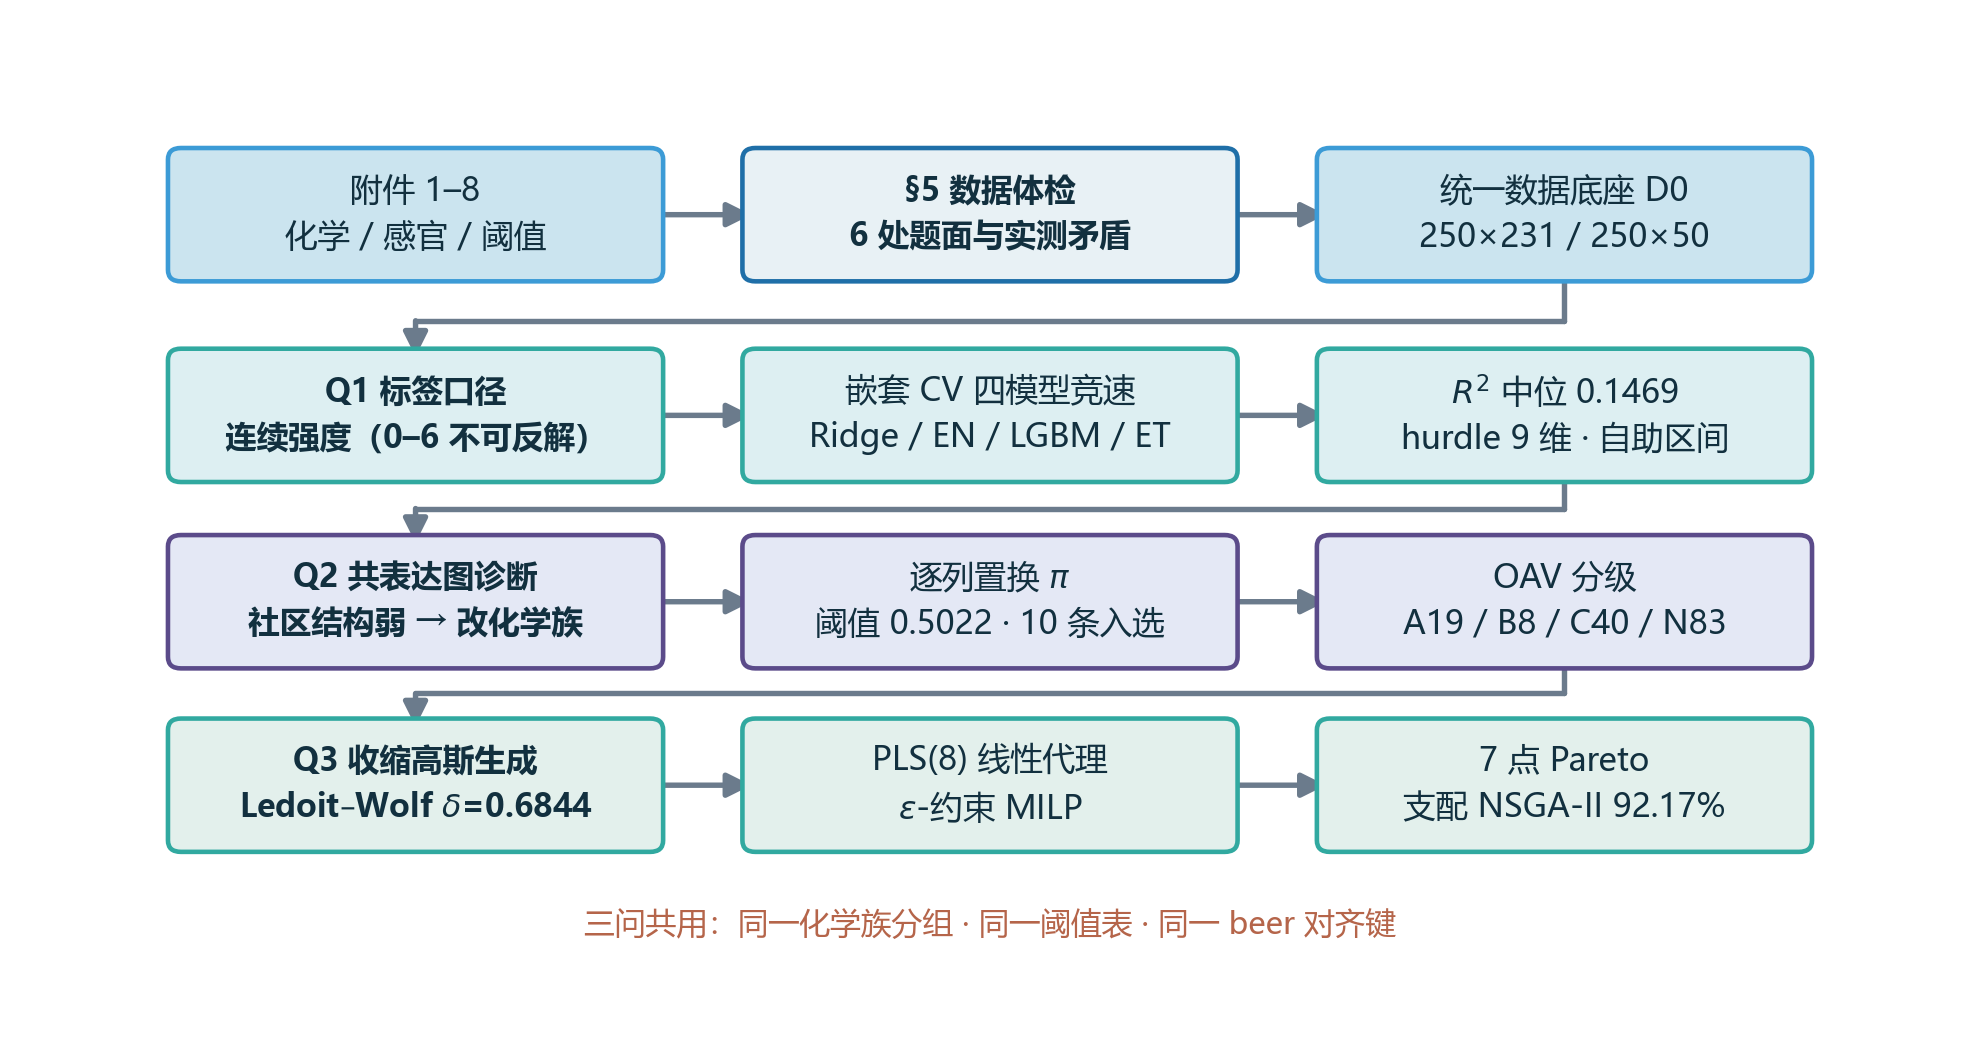
\includegraphics[width=\textwidth]{figures/fig_flow.png}
\caption{全文技术路线}
\label{fig:flow}
\end{figure}

\subsection{问题一的分析}

题目要求以附件1 的化合物数据为基础，给出附件3 中定义的 Aroma 与 Flavour 两套感官项的 0--6 分评分。这件事表面上是回归，实际有三层障碍。

第一层是标签不能直接用。附件4 给出的 50 个感官项并不是 0--6 的整数分，而是经过中心化的连续值：取值范围 $-2.151$ 到 $6.172$，六成是负数，每一列的不同取值少则 106 个、多则 250 个。本文试过把所有取值平移成非负数再四舍五入，结果中位 53.2\% 的样本被压到 0 分，分出来的等级几乎没有意义（第六章表~\ref{tab:q1grade} 有对照）；也试过先假定一个比例尺再取整，同样找不到稳定的比例尺。所以整数分不能从数据直接还原，只能另外定一套映射规则，并把这条限制写进论文。

第二层是样本少、特征多。250 款酒对 231 个化学指标，比值接近 1。这种规模下任何模型都能把训练集拟合得很好，所以评估方法比模型本身更关键，必须用嵌套交叉验证把选模型与报分数分开，组织方式见 6.3 节。

第三层是化学谱究竟能解释多少感官。同一数据集的原论文\cite{schreurs2024}报告梯度提升在训练感官面板上的多输出 $R^2$ 约 0.21 到 0.22，本文把它当作可比的参照水平：结果远低于它说明实现有问题，接近它则说明这是数据本身的信息量上限，换更复杂的模型也不会有实质改善。

据此确定了做法。候选模型取四个：岭回归与弹性网\cite{zou2005}代表线性方法，可解释性好但抓不住非线性；LightGBM 与 ExtraTrees 代表树集成，能抓非线性与交互，但在 250 个样本上容易过拟合。四个模型放进同一个嵌套交叉验证里横向比较，每个感官项各自取内层表现最好的那一个，而不是全篇强推一个模型。另外，有些感官项有大量样本压在最低值（例如 barnyard 有 47.6\% 的样本落在最小值附近），这类项用普通回归会把“没尝出来”和“尝到了但很弱”混在一起，本文对它们额外加一层“先判断有没有、再判断有多强”的两段式结构。

\subsection{问题二的分析}

题目要求用附件2 的相关矩阵建化合物网络，结合附件1 的特征，给出每个感官项最关键的三类化合物，并论证结果稳定、化学上讲得通。

先说一个容易走错的地方。附件8 里已经放了两张现成的化合物重要性排序 MDI 与 SHAP。直接取用最省力，但不适用：它们是全部 231 列对某一个综合目标的排序，不是对 50 个感官项分别排的，也不说明因果关系\cite{lundberg2017}；本文只留作最后的方向对照。

真正的难点是共线。231 个指标里有 219 个的方差膨胀因子大于 10，但只有 6 对相关系数的绝对值超过 0.9。这说明共线是一大片弱相关的累积，不是少数几列重复。因此逐列打乱不可用：被打乱的列会被同族其余列顶替，重要性系统性偏小\cite{strobl2008}。本文改为按附件8 的化学来源分组、同族一起打乱。

稳定性是题目点名要求的内容，本文用两种方式量化：一是自助重采样 200 次，每次重做“打乱—排序”，统计每个化合物进入前三名的次数比例；二是换模型后各排一次前十名，模型取 LightGBM、ExtraTrees 与岭回归，两两计算 Jaccard 系数。前者衡量换一批样本还稳不稳，后者衡量换一个模型还稳不稳。显著性阈值也不手工设定，而由稳定选择的有限样本界反解（见 7.3 节）\cite{meinshausen2010}。

最后要有化学上的说服力。本文用气味活性值\cite{grosch1994}判断，即浓度除以该物质的香气阈值，据以核查：统计上重要的化合物，是否真的浓到能被闻到，并与已报道的啤酒气味活性物清单\cite{kishimoto2018} 对照。这一步会否掉一部分结果，但否掉是应该的。

\subsection{问题三的分析}

题目要求以风格为条件学一个生成模型，在给定风格下生成合理的化合物谱并给出感官画像，再做跨风格迁移且保证缺陷物不恶化。

生成这一步的困难在样本量。22 个风格里最小的只有 3 款酒，即 Faro 风格，多数不超过 20 款。条件变分自编码器、条件生成对抗网络这类方法用在这种规模上无法估计条件分布\cite{xu2019}，本文把它们作为对照并在论文中明确写“不适用”，不作为主方法。实际采用的做法更朴素：在每个风格内部估计一个多元正态分布，协方差用 Ledoit--Wolf 收缩法\cite{ledoit2004}估计。收缩的意义是，样本少的时候直接用样本协方差会严重高估方差方向，收缩后向对角阵靠拢，生成样本不会离实测太远；收缩强度由数据算出，不手工设定。

生成之后要判断像不像。本文用最近邻距离检验：如果生成的样本与最近的实测样本距离远小于实测彼此之间的距离，说明它在复制；远大于则说明跑到了数据分布之外。两者都不可接受，理想情况是两者相当。

优化这一步要有感官目标。本文用偏最小二乘回归\cite{wold2001}建立一个从化学谱到 50 项感官的线性映射，取 8 个成分，系数可以直接写进优化模型的约束。之所以选偏最小二乘而不选树模型，是因为后面要解的是线性混合整数规划，需要可线性化的结构，树模型无法写进规划。

三个目标分别是感官偏差、缺陷风险和改动代价，单位不同、不能相加，因此用 $\varepsilon$-约束法\cite{mavrotas2009}：先分别求三个单目标得到支付表，再在对缺陷风险和改动代价的限制下逐步收紧，逐点求最小的感官偏差。这里之所以不直接用 Gurobi 自带的多目标接口，是因为它只支持线性目标，而感官偏差含绝对值，需要先线性化并入约束。为了验证这套精确解是否值得，本文另外手写了一个 NSGA-II\cite{deb2002}作对照，用两套前沿的支配关系与超体积来判断。

%==============================================================================
% 三、模型假设
%==============================================================================
\section{模型假设}

本文只保留五条真正影响建模取法的假设。每条给出数据层面的依据，并注明它被哪一节用到；凡依据可实测的都附实测值。其余常规假设（如随机误差零均值）不单独列出。

\textbf{假设 1（量纲与缺失可分辨）}\quad 附件1 中经对数变换的化学列底数为 10 且可逐列判定；取值为地板值时表示低于检出限而非真实浓度，NaN 表示未测量。依据：附件8 的 Calibrated 表给出 70 个化学列的还原浓度，逐列对拍 37 列落在 $\log_{10}$ 域、33 列落在原始线性域、161 列无对照；地板值 $-1.817819$ 在 142 列上精确重复共 6807 次，而 NaN 只分布在 9 列、共 73 格，两者形态不同。\emph{用于}第五章：不做整列反变换、不删列，地板值保留、NaN 按列中位数填补。

\textbf{假设 2（感官强度连续）}\quad 附件4 的 50 个感官项是 7 点量表按品评员 z-score 后再按啤酒平均的连续强度，项间差异不含量纲差异。依据：50 列全部存在负下限，每列不同取值数中位 229，逐列仿射搜索的残差 0.11--0.15，落不到整数格点；平移后直接取整会使 53.2\% 的样本压到 0 档。\emph{用于}第 6.2 节：问题一按回归而非分类建模，0--6 分级留到第 6.8 节用分位映射处理。

\textbf{假设 3（样本独立、风格组内同质）}\quad 每款啤酒的化学谱与感官评分来自同一批次且样本间独立；同一风格内的化学谱可由单一多元分布刻画。依据：beer 列在附件1、4、7 中均唯一且 250 行顺序一致；对 22 个风格做 Kruskal--Wallis 检验，231 个特征中 205 个在 0.05 水平显著、148 个过 Bonferroni 校正，$\varepsilon^2$ 中位 0.1768。风格内样本数中位 11、最小 3，故风格层面的结论不外推到单个品牌。\emph{用于}第 6.3 节的交叉验证划分与第 8.2 节的风格内条件分布。

\textbf{假设 4（局部线性、代理只定向不定点）}\quad 在实测样本覆盖范围内化学谱到感官的映射可用线性结构近似，但线性代理只支撑“往哪个方向调”，不支撑“哪个点更好”。依据：嵌套交叉验证中弹性网在 6 项取胜、两类树模型在 44 项取胜，说明线性结构存在但非全局；偏最小二乘代理的绝对误差中位 0.4626、95 分位 1.4124、上界 3.1525，与相邻 Pareto 点之间的间隙同量级。\emph{用于}第 7.3 节改用树模型加逐列置换做归因，第 8.3 节用偏最小二乘的线性映射写入规划，第 8.5 节对前沿只做分段报告。

\textbf{假设 5（阈值判据有效）}\quad 缺陷化合物是否恶化，以其浓度与香气阈值之比是否上升为准，与阈值的绝对量级无关。依据：231 个特征中 43 个在附件8 或公开文献中有阈值，同单位直接相除不做量纲换算；余下 188 个无阈值，标为 N 档且不作化学结论。\emph{用于}第 7.4 节的气味活性值裁判（A/B/C/N 四档）与第 8.4 节缺陷物的软约束与上限约束。

%==============================================================================
% 四、符号说明
%==============================================================================
\section{符号说明}

为便于对照，全文主要符号列于表~\ref{tab:symbols}。未在此表中的一次性符号在首次出现处就地说明。

\begin{table}[htbp]
\centering
\small
\caption{主要符号说明}
\label{tab:symbols}
\begin{tabular*}{\textwidth}{@{\extracolsep{\fill}}p{1.5cm}p{9.3cm}p{2.6cm}@{}}
\toprule
\textbf{符号} & \textbf{含义} & \textbf{单位} \\
\midrule
$n,\ p,\ m$ & 样本数、化学特征维数、感官维数，其中 $n=250$、$p=231$、$m=50$ & -- \\
$c_{ij}$ & 第 $i$ 个啤酒第 $j$ 个化合物的浓度，已还原量纲 & mg/L 等 \\
$y_{is}$ & 第 $i$ 个啤酒第 $s$ 个感官维度的强度值 & 无量纲 \\
$X,\ Y$ & 化学特征矩阵与感官标签矩阵 & -- \\
$\phi_s$ & 第 $s$ 个感官维度的左尾占比，即与该列最小值相距 ≤0.15 的样本占比 & -- \\
$\pi_j$ & 化合物或化学族 $j$ 的置换重要性 & -- \\
$\pi_{\mathrm{thr}}$ & 置换重要性的入选频率阈值（非 FDR 控制值） & -- \\
$B,\ k$ & 自助重采样次数与 Top-$k$ 入选集合，其中 $B=200$、$k=3$ & -- \\
$O_{ij}$ & 化合物 $j$ 对感官维度 $i$ 的气味活性值 OAV & -- \\
$J(A,B)$ & 两个候选集合的 Jaccard 系数 & -- \\
$x_j,\ x^{0}_j$ & 问题三中化合物 $j$ 的优化值与原始值（$\log_{10}$ 域） & -- \\
$z_j$ & 化合物 $j$ 是否被改动的 0--1 决策变量 & -- \\
$\hat y_s(x)$ & 线性代理对第 $s$ 个感官维度的预测 & 无量纲 \\
$t_s$ & 目标风格的参考感官值（风格内中位数） & 无量纲 \\
$d_k,\ \tau_k$ & 缺陷物 $k$ 的浓度与其香气阈值 & $\mu$g/L 或 mg/L \\
$f_1,f_2,f_3$ & 感官偏差、缺陷风险、改动代价三个目标 & 无量纲 \\
$\varepsilon_2,\ \varepsilon_3$ & $\varepsilon$-约束法中 $f_2,f_3$ 的上界 & 无量纲 \\
\bottomrule
\end{tabular*}
\end{table}

%==============================================================================
% 五、数据预处理与探索性分析
%==============================================================================
\section{数据核验与预处理}

\subsection{附件的实测结构与题面差异}

八个附件逐行读取后，规模与题面描述并不完全一致。凡有出入处，本文以实测为准，并把差异与处理方式写在下面，避免后续建模建立在错误的量纲与标签之上。

附件1 是化学特征矩阵，$250\times234$，即 250 款酒、3 个元数据列加 231 个化学列。231 列里 5 个是由其他列算出的派生量，含热量值、总酸、总酯、酒花香气与硫化合物。这 5 列保留入模：附件2 的相关矩阵按 231 列给出，剔除派生量会使矩阵与特征表对不上，且派生量本身携带总量信息。231 列的尺度并不统一：37 列经与附件8 的 Calibrated 表逐列对照确认在 $\log_{10}$ 域，33 列确认是原始线性浓度，其余 161 列没有对照、只能按取值范围推定。此外 142 列的含量出现同一检出限地板值，9 列存在真实缺失。

附件2 是化合物相关矩阵，$231\times231$。题面称其为皮尔逊相关，实测是 Spearman：与附件1 重算的 Spearman 矩阵逐格比对，42642 个格子的中位绝对差为 $8.33\times10^{-17}$，与皮尔逊则相差 0.063。因此全文的相关性一律按 Spearman 处理。

附件3 是感官评分卡，题面说 10 个 sheet，实测 13 个。13 张表共 1260 条公式，缓存值全为 0，不提供真值，只提供评分卡结构，含 15 项 Aroma、15 项 Flavour 与 20 个打分项，本文只用其结构。

附件4 是感官标签，$250\times53$，即 3 个元数据加 50 个感官项。它是中心化后的连续强度值，不是 0--6 的整数分，这一点在第六章详述。

附件5 是感官之间的相关矩阵，$50\times50$，同样是 Spearman，行列名用论文长名。

附件6 是化合物与感官的交叉相关矩阵，题面说 $46\times50$，实测 $44\times50$。它只覆盖 $231\times50$ 个可能格子的 18.67\%，因此只作交叉校验，不能当作全量相关结构。

附件7 是论坛评论描述符，$250\times189$，3 列整列为空、可用 183 列，是真正的 $z$ 分数，列标准差中位 1.003。它与附件4 不同源，只用于外部效度检验。

附件8 是综合参考数据，7 个 sheet。其中阈值表 261 行里只有 43 行有数值，这是后文一半归因记录无法做化学判断的直接原因；化学来源标注覆盖 226 个实测特征、余下 5 个派生量归入其他族，用于问题二的分组；Calibrated 表是把 $\log_{10}$ 还原成浓度的官方对照，用于核定量纲；MDI 与 SHAP 两张表是现成的重要性排序，本文不采用，理由见第七章。

最后是题面把"226 种啤酒"写成样本数这一处。全部附件都是 250 行，226 实为化学指标数，本文一律以 250 为样本量。

\subsection{缺失与检出限的分离}

附件1 的缺失有两种不同机制，必须分开处理，这是全文建模的前提。

第一类是检出限截断。有 6807 个单元格的取值精确等于 $-1.817819$，即 $10^{-1.8178}\approx0.0152$，分布在 142 列上。其中 40 列有 30\% 以上的样本精确落在该列的最小值上；若只取最小值恰为检出限 $-1.817819$ 的那 142 列，仍有 35 列的地板值占比超过 30\%。最高的两列（甲基庚烯酮与柠檬烯）达 84.8\%。这表示该化合物低于检测限，是有效信息而非错误值，因此既不删除也不按均值填补。

第二类是真实缺失。按 231 个化学列统计，共 73 个单元格、9 列；去掉 5 个派生列后剩 60 个单元格、8 列，13 格差额全部来自 aroma\_hops\_sum 这一列。缺失最多的 amyl.acetate 占 27/250，且并非随机分布：Dubbel 组 4/10、Kriek 组 3/10、Blond 组 6/31。因此按列中位数填补，不用全表均值，避免把风格差异抹平。这类缺失规模小，不构成建模障碍。

第三类是感官侧的列内左尾。附件4 的标签不是原始 0--6 分值：文献\cite{schreurs2024}的方法写明，16 位品评员先按 7 点量表打分，再\textbf{按品评员做 z-score}（减均值、除标准差），最后按啤酒求平均；原文对此的表述是"Scores were scaled by standard deviation and mean-centered per taster. Values are represented as z-scores"。因此负值表示"低于该品评员的平均"，不是"没有尝到"；列最小值是 z 空间里的左尾，不是感官 0 分。

据此，本文把 $\phi_s$ 定义为\emph{左尾占比}，即与该列最小值相距不超过 0.15 的样本占比
\begin{equation}
  \phi_s=\frac{1}{n}\sum_{i=1}^{n}\mathbb{I}\left(y_{is}\le \min_{i'}y_{i's}+0.15\right),
\end{equation}
作为各列分布左尾厚度的度量，供问题一判断是否需要单独处理高左尾项。图~\ref{fig:q0missing} 给出这两类问题的分栏对比：前者稀疏且集中在少数列，后者是整列高比例的同一取值。

\begin{figure}[htbp]
\centering
\begin{subfigure}[t]{0.48\textwidth}
\centering
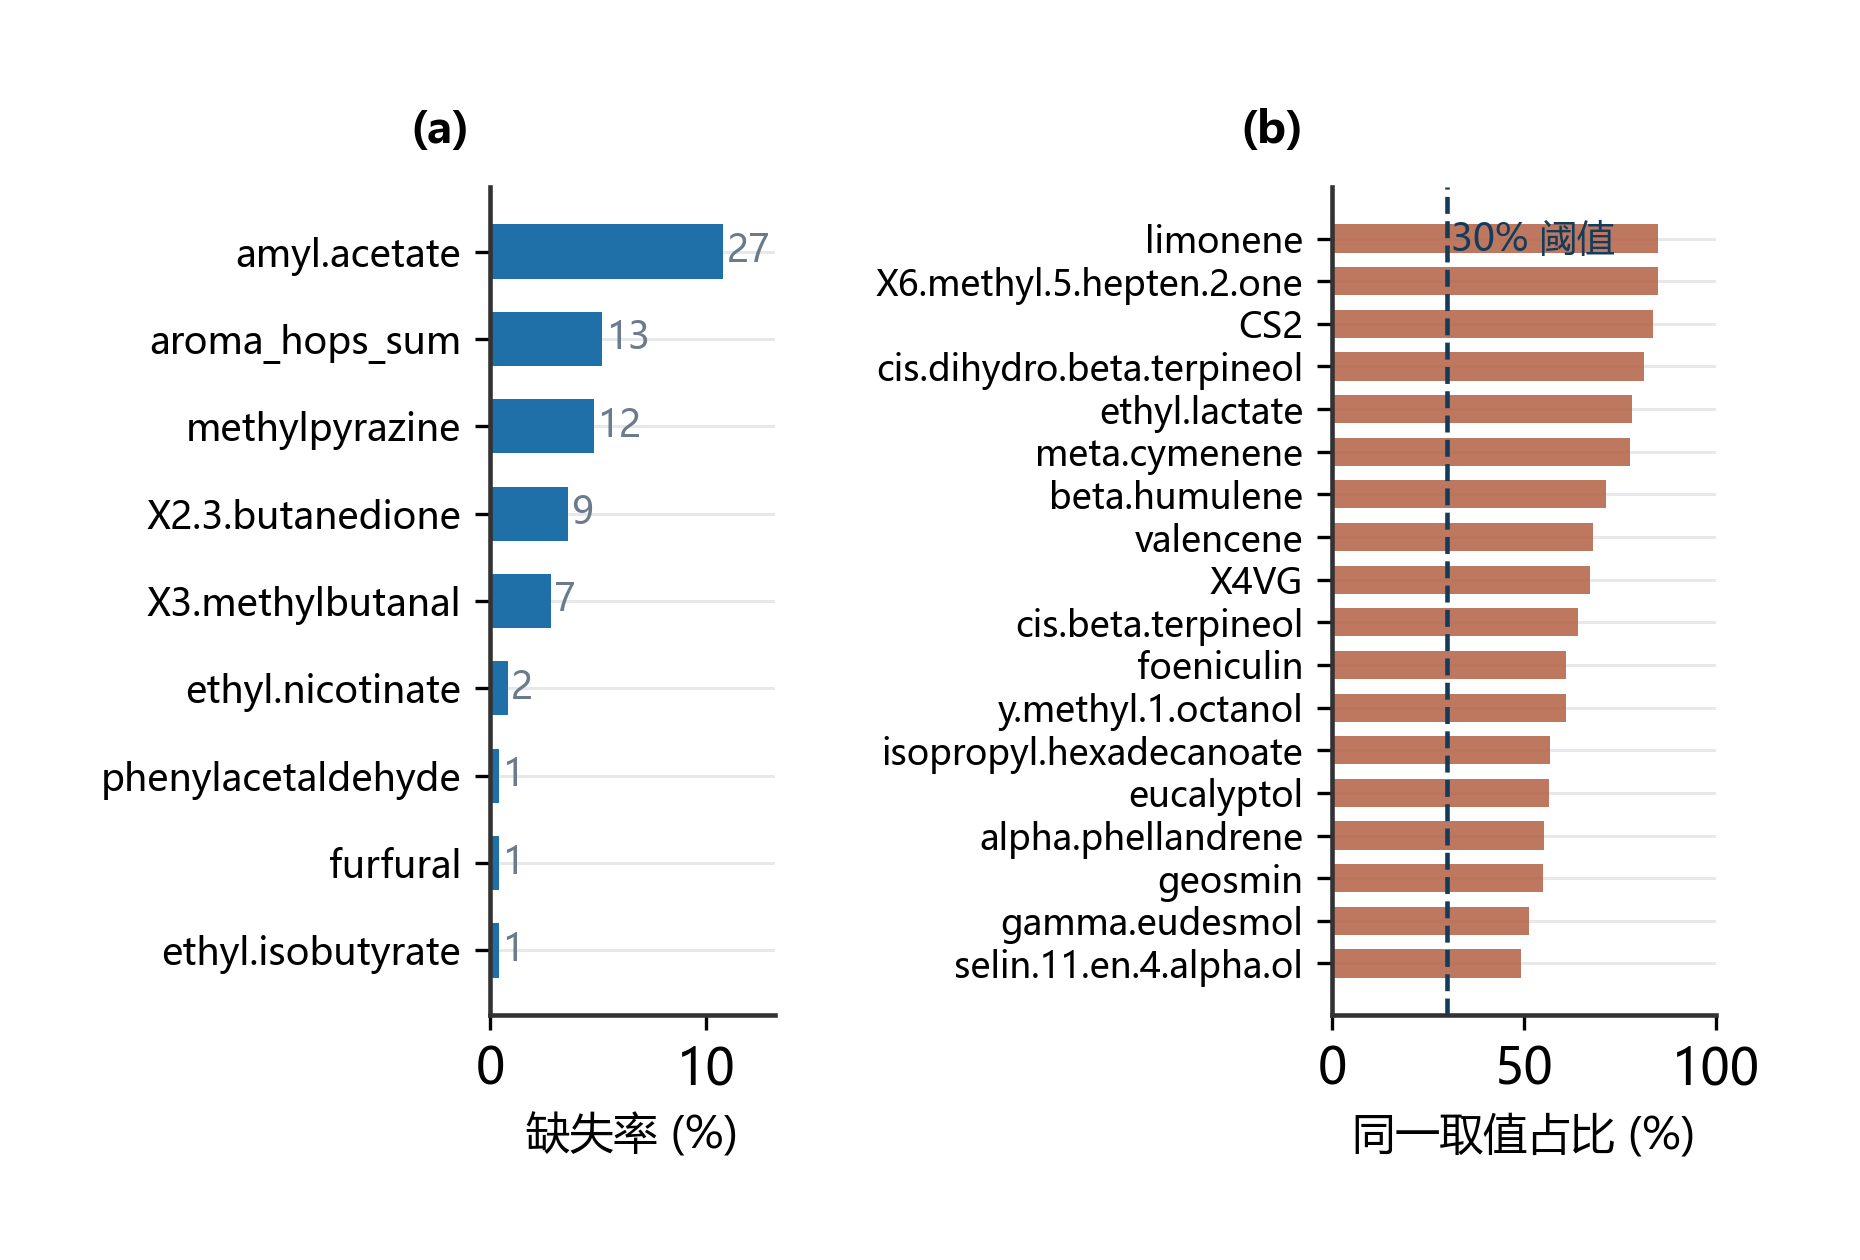
\includegraphics[width=\linewidth]{figures/fig_q0_missing.png}
\caption{数据缺陷的分栏对比。左图为真实缺失列及其缺失率，右图为检出限地板值列，同一取值占比超过 30\% 的列按虚线标出}
\label{fig:q0missing}
\end{subfigure}
\hfill
\begin{subfigure}[t]{0.48\textwidth}
\centering
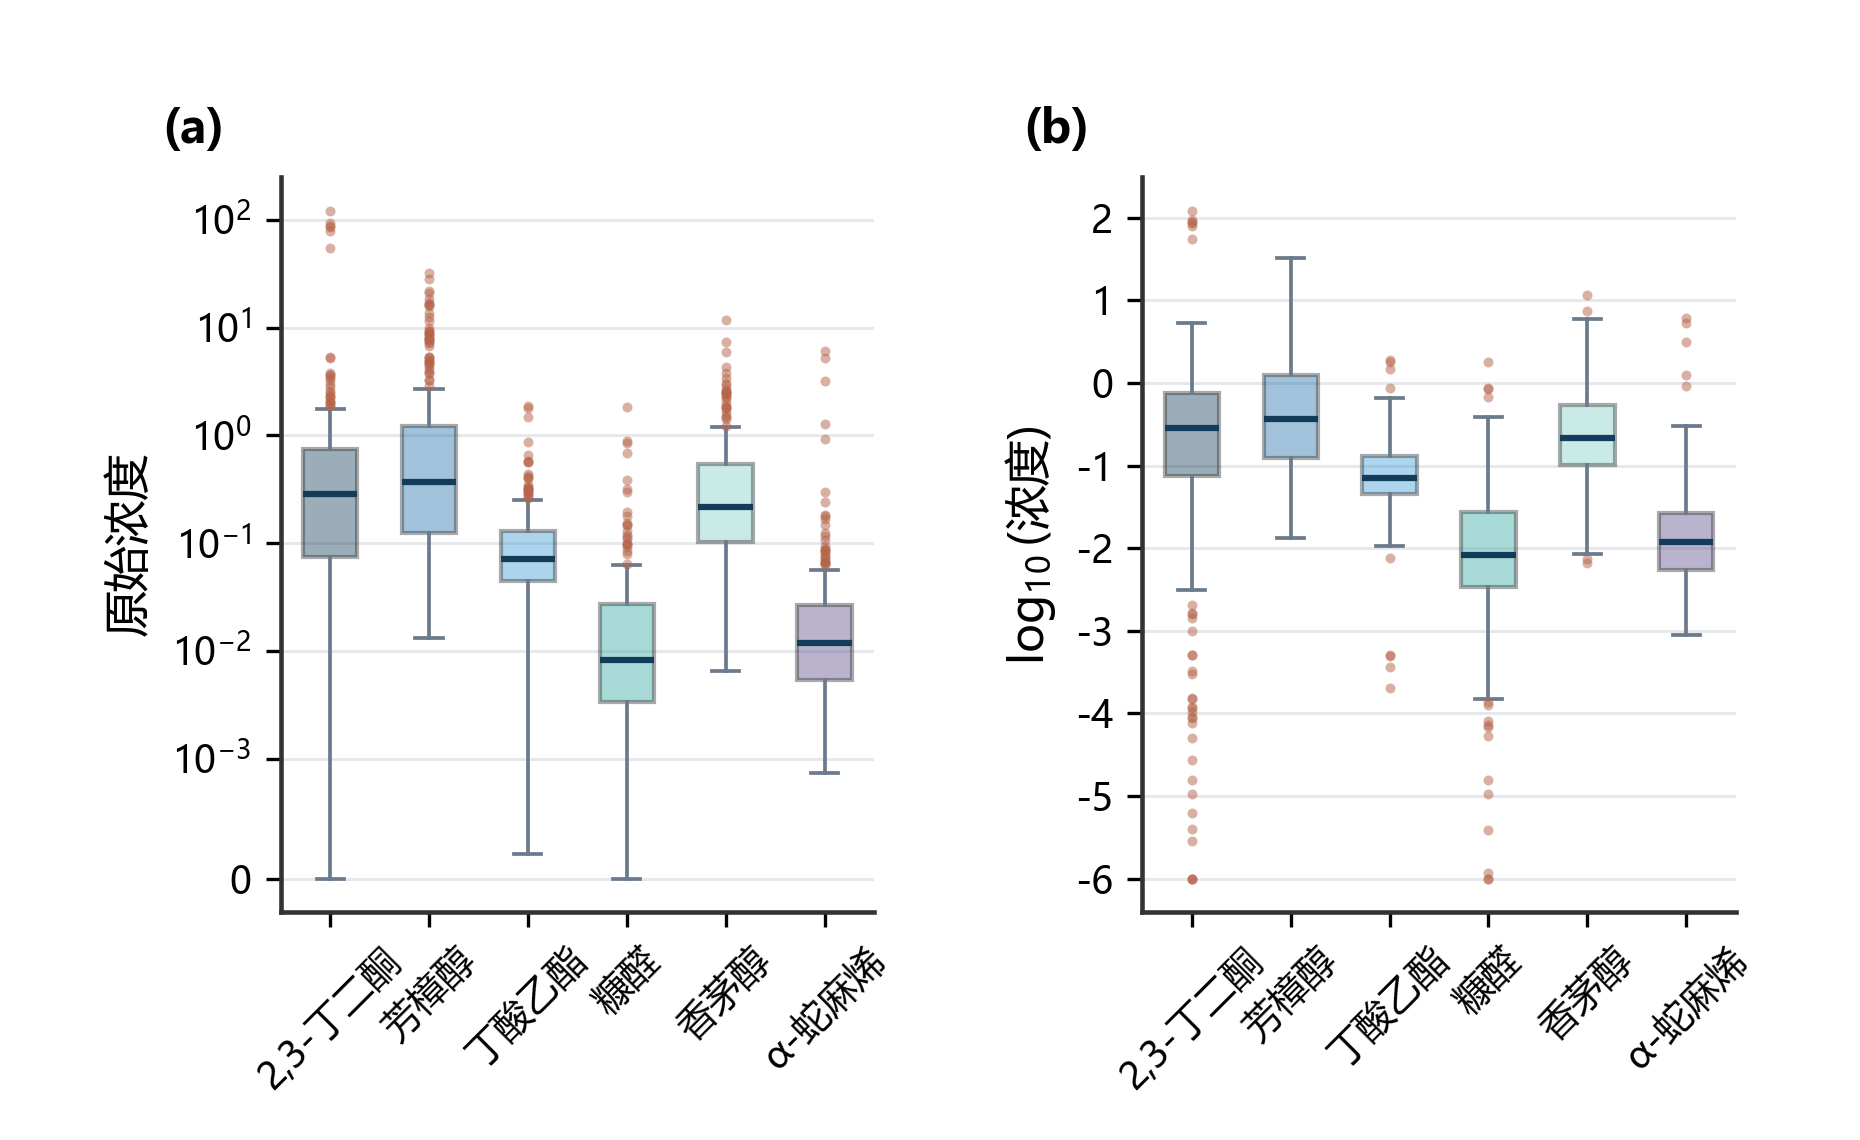
\includegraphics[width=\linewidth]{figures/fig_q0_box_before_after.png}
\caption{量纲统一前后的分布对比。左图为原始浓度对称对数轴，右图为 $\log_{10}$ 域}
\label{fig:q0box}
\end{subfigure}
\caption{数据层面的两处缺陷与处置。左图为真实缺失列的缺失率，右图为量纲统一前后的分布对比（左半为原始浓度对称对数轴，右半为 $\log_{10}$ 域）}
\end{figure}

\subsection{量纲与共线结构}

231 个特征的尺度并不统一，实测分三类：33 列经与附件8 的 Calibrated 表逐列对照，确认是原始线性浓度，相对误差低于 $10^{-3}$ 且列内无零值格；37 列确认在 $\log_{10}$ 域；其余 161 列在 Calibrated 表中没有对照，只能按取值范围判断——145 列含负值，负值只能来自对数域，另 15 列因原始浓度全部大于 1 而取正值、1 列全非负且最小值小于 1 而判为线性域。合计 182 列在 $\log_{10}$ 域、49 列为线性尺度。这个分域不是文字细节：决策变量同时含两种域时，任何“浓度改变量”的求和都必须先归一，具体做法见第八章对 $f_3$ 的说明。

这一点直接决定建模时的处理方式。本文不对任何列做 $10^{x}$ 反变换：反变换后 6 个代表化合物的浓度跨度从 $5.9\times10^{-8}$ 到 121.7，跨越 9 个数量级，标准化虽能把各列压到零均值单位方差，但极端列仍会主导线性模型的系数；保持 $\log_{10}$ 域可把有效跨度压到 6 个数量级左右。图~\ref{fig:q0box} 的左栏即反变换后的原始浓度分布，必须用对称对数轴才能显示，右栏为本文实际使用的 $\log_{10}$ 域分布。



共线的实测结果是本文两处建模选择的直接依据。231 列的方差膨胀因子中位数 35.96、最大 964.91，219 列超过常用阈值 10，其中 31 列超过 100；Spearman 版本的有效秩仅 20.62，条件数 $2.04\times10^5$，需 67 个主成分才达到 90\% 方差，第一主成分只解释 14.48\%。但与此同时，只有 6 对特征的相关系数绝对值超过 0.9，特征对的中位绝对相关仅 0.1293。两者合起来说明：这里的共线是一大片弱相关的累积，不是少数几对强冗余。因此“按方差膨胀因子删变量”会把 219 列删光，正确做法是在建模层面处理——问题二按逐列置换估计重要性，问题三用收缩协方差与偏最小二乘。

\subsection{相关结构与风格差异}

特征与感官之间的关联本身很稀。11550 个特征--感官格子中，中位绝对相关仅 0.0878，超过 0.5 的只有 44 格（0.38\%），超过 0.7 的仅 3 格。表~\ref{tab:senscorr} 列出最强的 5 对，全部可以作化学解释：乙醇对应酒精感与酒体，苦度对应苦味，色度对应焦香麦芽香，辛酸乙酯对应二氧化碳感。

\begin{table}[htbp]
\centering
\footnotesize
\caption{特征与感官的最强相关对，按 Spearman 相关排序}
\label{tab:senscorr}
\begin{tabular*}{\textwidth}{@{\extracolsep{\fill}}llc}
\toprule
\textbf{感官项} & \textbf{化学特征} & $\rho$ \\
\midrule
alcohol & ethanol (v/v) & 0.8171 \\
body & ethanol (v/v) & 0.7191 \\
bitternes & bitterness & 0.6822 \\
A\_malt\_cara & color EBC & 0.5636 \\
co2 & ethyl\_octanoate & 0.5527 \\
\bottomrule
\end{tabular*}
\end{table}

风格的区分力则很强。对 22 个风格做 Kruskal--Wallis 检验，231 个特征中 205 个在 0.05 水平显著、148 个经 Bonferroni 校正后仍显著，效应量 $\varepsilon^2$ 中位 0.1768、最大 0.7910。这既说明风格标签可以作为条件变量使用，这也是问题三可行的依据，也说明若交叉验证不按风格分层，某些折内将不含小类样本，指标会失去意义。

与官方文件的交叉校验达到机器精度：附件2 的 44732 个可比对格子中位绝对差 $8.33\times10^{-17}$，附件6 的 2156 个格子为 $5.55\times10^{-17}$，一致性均为 1。这说明本文的相关矩阵重新计算结果无误，前述共线结构不是实现错误造成的假象。

%==============================================================================
% 六、问题一的模型建立与求解
%==============================================================================
\section{问题一：感官评分的预测与分级}

\subsection{建模思路}

问题一要把 231 个化学指标映射到 50 个感官项的强度值。建模前先核实三件事，它们决定了模型的选择。

第一，输出不是整数等级。附件4 的 50 个感官项取值在 $-2.151$ 到 $6.172$ 之间，六成是负数，每一列的不同取值少则 106 个、多则 250 个。这说明它是中心化后的连续强度，不是 0--6 的评分。把取值平移到非负再四舍五入，中位 53.2\% 的样本会被压到 0 分，等级信息几乎全部丢失。因此本问按\emph{连续值回归}建模，等级放到最后用分位映射单独解决。

第二，样本量与特征数几乎相等。250 款酒对 231 个指标，比值接近 1。这种规模下任何模型都能把训练集拟合到 $R^2>0.9$，报出的精度若不与选择过程隔离，就只是挑选的结果。本文采用\emph{外层 5 折评估、内层 5 折选模型}的嵌套交叉验证，组织方式见 6.3 节。

第三，目标之间难度差异极大。同一数据集的原论文\cite{schreurs2024}报告梯度提升在训练感官面板上的多输出 $R^2$ 约为 0.21，本文以此为参照上限：结果远低于它说明实现有问题，接近它则说明这是数据本身的信息量边界。

基于这三点，本问取四个回归模型并列比较，每个感官项各自取内层最优，而不预先指定其中任何一个。

\begin{itemize}
  \item \textbf{岭回归}：线性模型加 $\ell_2$ 惩罚，把系数整体压小，适合处理共线，但抓不住非线性。
  \item \textbf{弹性网}：线性模型同时加 $\ell_1$ 与 $\ell_2$ 惩罚，既压系数又做变量筛选，输出比岭回归稀疏、更易解释。
  \item \textbf{LightGBM}：梯度提升树，逐轮拟合前一轮的残差，按直方图选分裂点，能刻画非线性与特征交互。
  \item \textbf{ExtraTrees}：极端随机树，在随机切分点上建大量树后取平均，方差远低于单棵树，在 250 个样本上更稳。
\end{itemize}

此外，50 项里有 9 项的地板效应占比超过 0.30，即三成以上样本挤在该项最低值附近，barnyard 达 0.476。这类项用普通回归会把“没有感知到”与“感知到但很弱”混为同一件事。对它们本文改用\emph{两段式模型}：先用梯度提升分类器判断该项是否被感知，再用回归器在已感知样本上估计强度，两者相乘。被划入两段式的是 acetic、lactic、coriander、A\_malt\_burn、orange、clove、barnyard、F\_hops\_tropical、stale\_hops 共 9 项，以酸味、香料与缺陷味为主。

\subsection{模型建立}

设第 $i$ 个样本的化学特征为 $\boldsymbol{x}_i\in\mathbb{R}^{231}$，第 $s$ 个感官项的强度为 $y_{is}$。四个模型中，岭回归与弹性网有显式目标函数，树模型没有。

岭回归最小化残差平方和加 $\ell_2$ 惩罚
\begin{equation}
  \hat{\boldsymbol\beta}^{\mathrm{ridge}}_s=\arg\min_{\boldsymbol\beta}\ \frac{1}{2N}\lVert \boldsymbol{y}_s-\boldsymbol{X}\boldsymbol\beta\rVert_2^2+\lambda\lVert\boldsymbol\beta\rVert_2^2 .
\end{equation}
弹性网在惩罚项里再加一个 $\ell_1$ 分量
\begin{equation}
  \hat{\boldsymbol\beta}^{\mathrm{enet}}_s=\arg\min_{\boldsymbol\beta}\ \frac{1}{2N}\lVert \boldsymbol{y}_s-\boldsymbol{X}\boldsymbol\beta\rVert_2^2
  +\lambda\left(\alpha\lVert\boldsymbol\beta\rVert_1+\frac{1-\alpha}{2}\lVert\boldsymbol\beta\rVert_2^2\right),
\end{equation}
其中 $\lambda$ 与 $\alpha$ 都在内层交叉验证上选。LightGBM 与 ExtraTrees 不写目标函数：前者以均方误差为损失逐轮拟合负梯度，后者对每个节点在随机阈值上切分、对多棵树取算术平均。

两段式模型的预测值是两个阶段的加权混合，而非相乘
\begin{equation}
  \hat y_{is}=\left(1-\hat\pi_{is}\right)\bar y_s^{\text{floor}}+\hat\pi_{is}\,\hat\mu_{is},\qquad
  \hat\pi_{is}=\Pr\left(y_{is}>y_s^{\min}\mid \boldsymbol{x}_i\right),
\end{equation}
其中 $\hat\pi_{is}$ 由梯度提升分类器给出，$\hat\mu_{is}$ 由回归器在 $y_{is}>y_s^{\min}$ 的样本上给出，$\bar y_s^{\text{floor}}$ 为左尾样本（$y\le y_s^{\min}+0.15$）的强度均值。此处不用 $\hat\pi\hat\mu$ 的乘积形式，是因为乘积会把左尾样本的预测强行拉到 0，而实测中这类样本的强度并不为 0（只是集中在列最小值附近），相乘会系统性低估其强度；加权混合保留了“落在左尾时取左尾均值”这一含义，也让 $\hat\pi$ 退化为 0/1 时连续过渡到单段回归。需要说明的是，这里的 $\hat\pi$ 是“强度高于左尾窗”的概率，不是“是否感知到”的概率——附件4 的标签已按品评员做过 z-score，负值代表低于该品评员的平均，不代表没有尝到（见 5.3 节）。

评价用决定系数与平均绝对误差
\begin{equation}
  R^2_s=1-\frac{\sum_i\left(y_{is}-\hat y_{is}\right)^2}{\sum_i\left(y_{is}-\bar y_s\right)^2},
  \qquad
  \mathrm{MAE}_s=\frac{1}{n}\sum_i\left|y_{is}-\hat y_{is}\right|,
\end{equation}
并用 1000 次自助重采样在折外预测上给出 $R^2$ 的 95\% 置信区间。

\subsection{模型求解}

\noindent\textbf{交叉验证的组织方式}\quad 普通 5 折交叉验证的缺陷在于，选模型的数据与报分数的数据是同一批，四个模型里挑最好的那个，报出的分数就已经带上了挑选的痕迹；模型越多、特征越多，这种乐观偏差越大。本问有 250 个样本、231 个特征，若用普通 5 折，报出的 $R^2$ 会系统性偏高。

嵌套交叉验证把它拆成两层。外层 5 折只做一件事：把 250 个样本切成训练集 200 个与评估集 50 个。内层 5 折在训练集的 200 个样本内部再切一次，用内层 5 折的折外预测算出四个模型各自的 $R^2$，取最高的那个作为本折的选定模型。选定之后，用这 200 个样本全量重训该模型，再预测被留出的 50 个样本。评估集从头到尾不参与任何选择，因此报出的数才是泛化误差的无偏估计。代价是训练次数乘 5。

\noindent\textbf{四个模型的具体设置}\quad 四个模型的超参在建模前固定，不在交叉验证里搜索。这样做有两个考虑：一是 250 个样本上做超参网格，搜出来的最优值本身不稳定，反而增加选择偏差；二是固定超参后，四个模型之间的差异只来自模型族本身，比较结果更干净。具体取值见表~\ref{tab:q1hyper}。

\begin{table}[htbp]
\centering
\footnotesize
\caption{问题一四个候选模型的超参设置，建模前固定，不在交叉验证内搜索}
\label{tab:q1hyper}
\begin{tabular*}{\textwidth}{@{\extracolsep{\fill}}llp{7.4cm}@{}}
\toprule
\textbf{模型} & \textbf{类型} & \textbf{超参取值} \\
\midrule
岭回归 & 线性，$\ell_2$ 正则 & $\alpha=10$ \\
弹性网 & 线性，$\ell_1+\ell_2$ 正则 & $\alpha=0.05$，$\ell_1$ 比例 $0.5$，最大迭代 5000 \\
LightGBM & 梯度提升树 & 150 棵树，叶数 7，最小叶样本 8，学习率 0.06，行采样 0.8，列采样 0.6，$\ell_2$ 惩罚 1.0 \\
ExtraTrees & 极端随机树 & 200 棵树，每节点随机特征数 $\sqrt{p}$，最小叶样本 3 \\
\bottomrule
\end{tabular*}
\end{table}

标准化在每一折内部单独做：用训练折的中位数填补缺失、用训练折的均值与标准差做标准化，再把同一套参数用到评估折。若改用全表均值填补，评估折的信息就会提前泄露进训练。

两段式模型只在 9 个左尾占比超过 0.30 的感官项上启用，其分类头与回归头分别取与表中四个模型对应的组合，例如 LightGBM 分类配 LightGBM 回归、逻辑回归配岭回归，同样在内层 5 折里择优。

\noindent\textbf{实际计算量}\quad 按上述组织，全部计算量为外层 5 折、50 个感官项、4 个模型与内层 5 折的乘积，再加 50 次全量重训，共 5250 次模型拟合；两段式项每次拟合含分类与回归两个头，折算后实际拟合约 6100 次。区间估计在折外预测上做 1000 次自助重采样，每个感官项 1000 次、共 5 万次重采样，这一步只做排序与分位数计算，不再重训模型。

随机种子统一取 2026，树的并行度设为 4 进程，全部 50 项在单机串行跑完，耗时 273.6 秒，可作为复现的基准。

\subsection{结果分析：总体精度}

50 项的嵌套交叉验证结果为：$R^2$ 中位 0.1469、均值 0.2223；49 项为正，14 项超过 0.3、6 项超过 0.5、19 项低于 0.10；32 项的自助区间下界大于 0。区间宽度中位 0.1936，远大于 1000 次重采样的蒙特卡洛噪声，约 0.006，说明区间本身是稳的。图~\ref{fig:q1forest} 给出逐项的 $R^2$ 与区间，按数值排序。

\begin{figure}[htbp]
\centering
\begin{subfigure}[t]{0.48\textwidth}
\centering
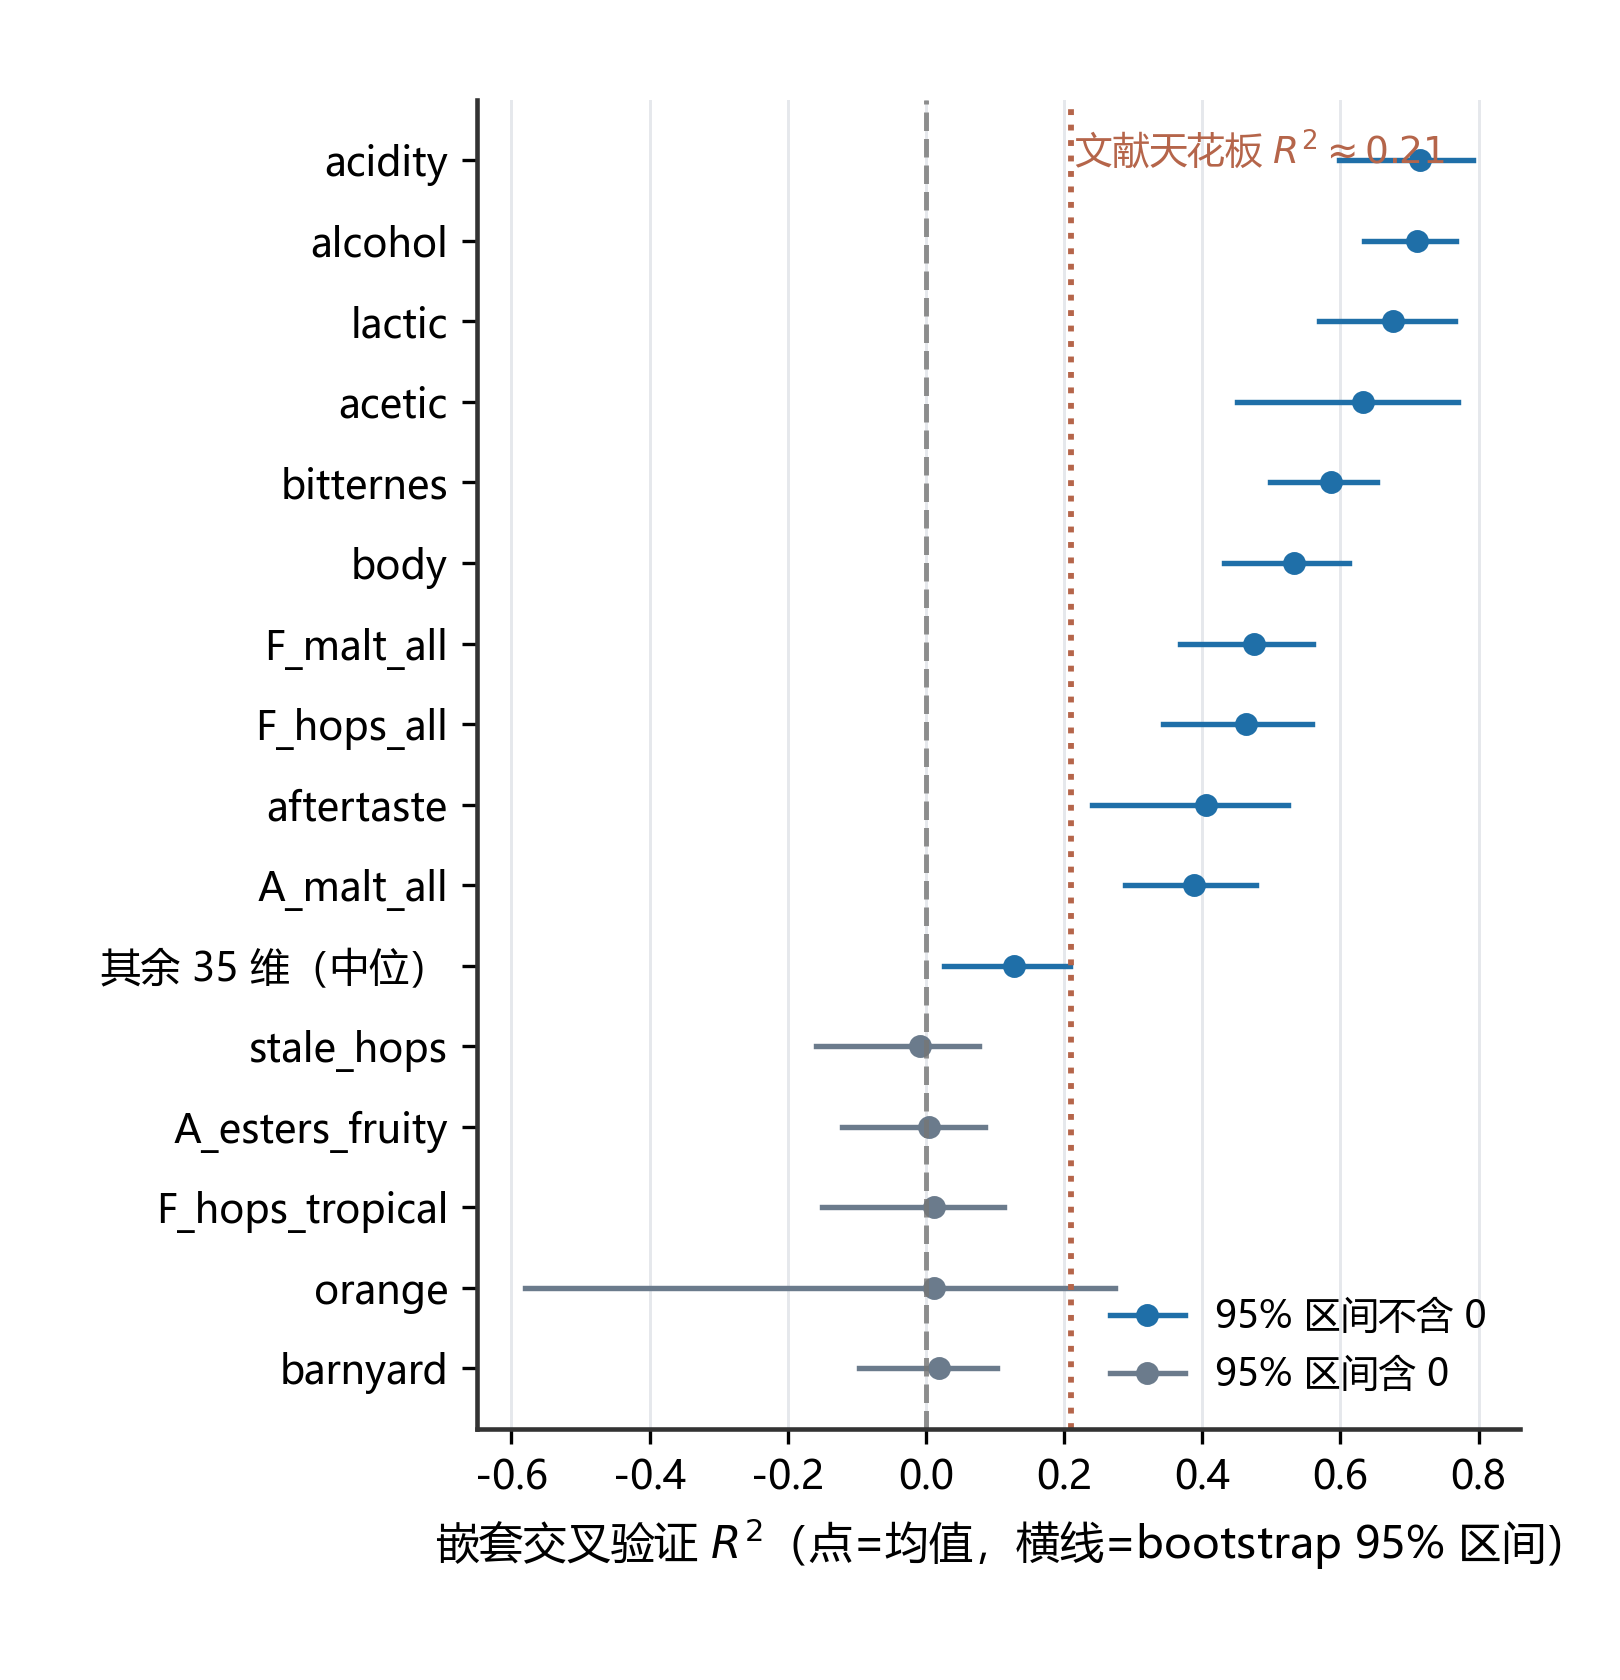
\includegraphics[width=\linewidth]{figures/fig_q1_r2_forest.png}
\caption{50 个感官项的 $R^2$ 与自助 95\% 区间。蓝点表示区间不含 0，灰点表示区间含 0}
\label{fig:q1forest}
\end{subfigure}
\hfill
\begin{subfigure}[t]{0.48\textwidth}
\centering
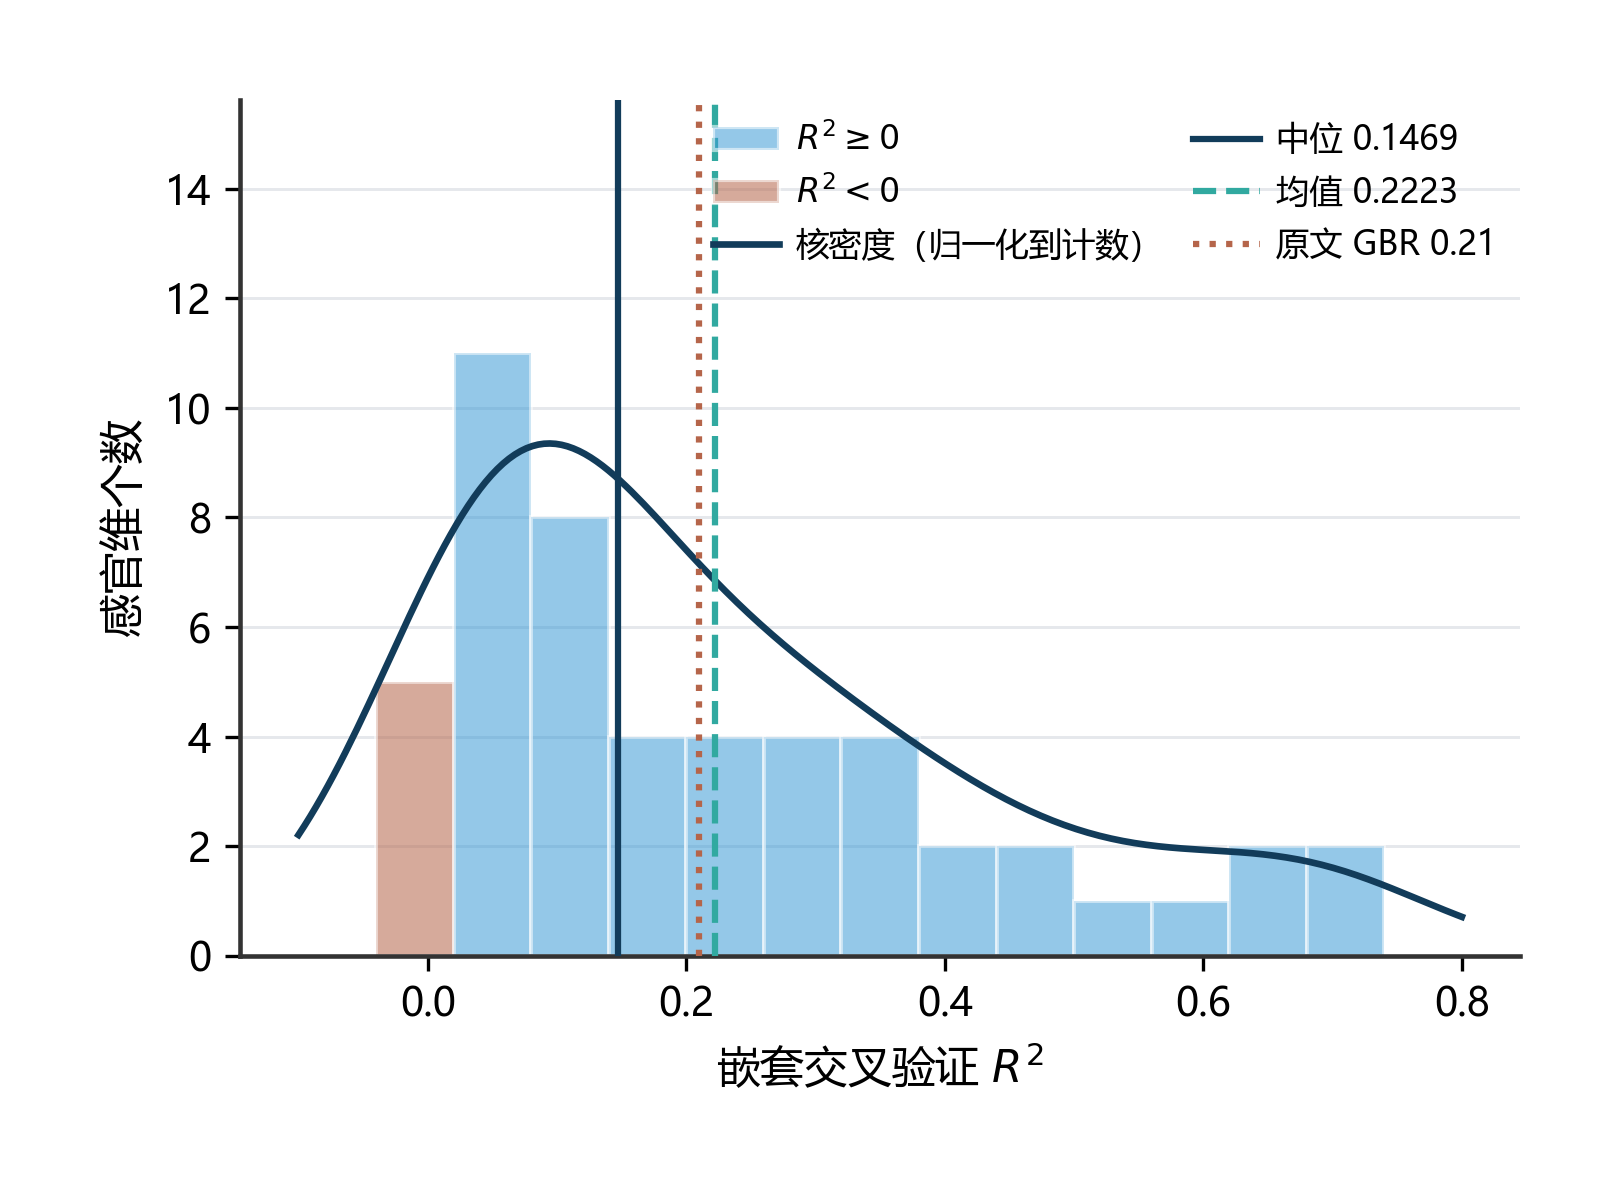
\includegraphics[width=\linewidth]{figures/fig_q1_r2_dist.png}
\caption{$R^2$ 的分布，竖线为中位数、均值与文献报道的梯度提升水平}
\label{fig:q1dist}
\end{subfigure}
\caption{问题一的 $R^2$ 结果。左图为 50 个感官项的 $R^2$ 与自助 95\% 区间，蓝点为区间不含 0；右图为 $R^2$ 的分布，三条竖线分别是中位数 0.1469、均值 0.2223 与文献报道的梯度提升水平 0.21}
\end{figure}

\subsection{结果分析：逐项结果与模型分工}

逐项看是散点，整体看是分布。图~\ref{fig:q1dist} 把 50 个 $R^2$ 叠成一张直方图并叠加核密度，三条竖线分别是中位数 0.1469、均值 0.2223 与文献\cite{schreurs2024}报道的梯度提升水平 0.21。中位比均值低 0.0754 是右偏的直接证据：多数项挤在 0.10 到 0.20 之间，少数理化直连的项把均值拉了上去，其中酸度 0.7149、酒精 0.7108、乙酸 0.6326、乳酸 0.6768。均值 0.2223 与文献的 0.21 几乎重合，说明整体信息量没有被浪费；而中位偏低说明这个均值是靠少数项撑起来的，不代表普遍水平。



四个模型被选中的次数说明了各自的分工：ExtraTrees 24 次、LightGBM 20 次、弹性网 6 次、岭回归一次也没有胜出。这个分布与 5.3 节测到的共线结构吻合——219 列的方差膨胀因子大于 10 时，纯岭惩罚压不住系数，树模型靠分裂绕开了这个问题，而弹性网的 $\ell_1$ 分量能在 231 列里挑出少数有用的列，所以在 body、F\_malt\_all、A\_malt\_all 这类信号稀疏的项上胜出。

可预测性最高的是 acidity 与 alcohol,$R^2$ 分别为 0.7149 与 0.7108。这两项对应酸度与乙醇浓度的直接化学测量，机理清楚，模型学到的基本上是线性关系。表~\ref{tab:q1} 列出前 10 项，其中 acetic 与 lactic 的地板效应占比高达 0.61 与 0.69，是靠两段式模型才取得 0.63 与 0.61 的——若用单段回归，这两项会被“大量样本压在最低值”拖垮。

\begin{table}[htbp]
\centering
\footnotesize
\caption{问题一前 10 个感官项的嵌套交叉验证结果}
\label{tab:q1}
\begin{tabular*}{\textwidth}{@{\extracolsep{\fill}}lcccc}
\toprule
\textbf{感官项} & \textbf{选中模型} & $R^2$ & \textbf{95\% 区间} & \textbf{MAE} \\
\midrule
acidity & LightGBM & 0.7149 & $[0.598,\ 0.791]$ & 0.2995 \\
alcohol & LightGBM & 0.7108 & $[0.634,\ 0.767]$ & 0.3268 \\
acetic & LightGBM（两段式） & 0.6326 & $[0.450,\ 0.771]$ & 0.1934 \\
lactic & LightGBM（两段式） & 0.6768 & $[0.569,\ 0.767]$ & 0.1875 \\
bitternes & LightGBM & 0.5862 & $[0.498,\ 0.652]$ & 0.3693 \\
body & 弹性网 & 0.5328 & $[0.431,\ 0.613]$ & 0.3038 \\
F\_malt\_all & 弹性网 & 0.4750 & $[0.368,\ 0.560]$ & 0.4033 \\
F\_hops\_all & LightGBM & 0.4639 & $[0.344,\ 0.559]$ & 0.3975 \\
aftertaste & LightGBM & 0.4048 & $[0.240,\ 0.524]$ & 0.3597 \\
A\_malt\_all & 弹性网 & 0.3795 & $[0.278,\ 0.466]$ & 0.4414 \\
\bottomrule
\end{tabular*}
\end{table}

中位 0.1469 比文献报告的 0.21 低 0.06，但均值 0.2223 与文献持平。两个数一起看才有意义：均值持平说明整体信息量没有被浪费，中位偏低说明分布是右偏的——少数理化直连的项被解释得较好，多数香气项几乎不可解释。这不是实现问题，而是 250 个样本下各项信息量本身差异极大。

\subsection{结果分析：预测质量与残差诊断}

$R^2$ 只说明整体解释力，看不出误差是怎么分布的。预测质量比 $R^2$ 数字更直观。图~\ref{fig:q1reg} 用四项做对照：alcohol 与 acidity 的散点紧贴 $y=x$;bitternes 的秩相关仍有 0.74，但斜率明显小于 1，高苦度样本被系统性低估，这是折外预测向均值收缩的常见表现；F\_esters\_flower 的散点是一团水平云，$R^2$ 只有 0.0293，模型对这一项没有解释力。越是贴近对角线的项，其 Top-3 归因才越可信，这一点在第七章会用到。

\begin{figure}[htbp]
\centering
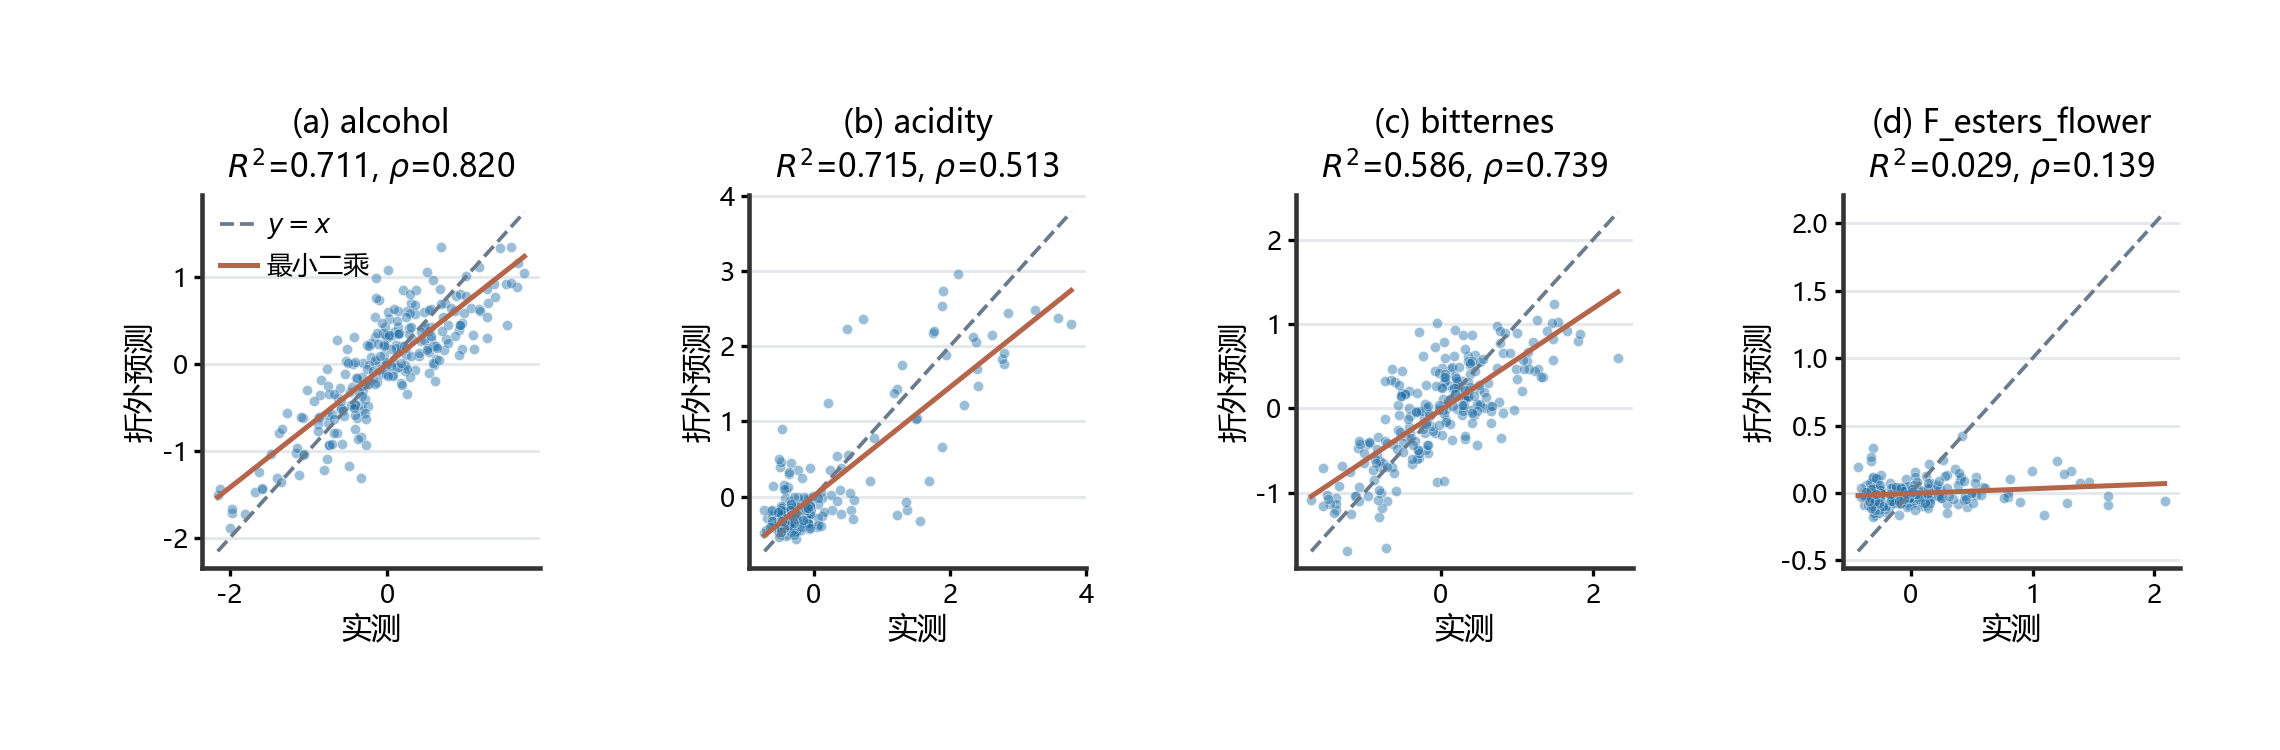
\includegraphics[width=0.86\textwidth]{figures/fig_q1_reg_fit.png}
\caption{四个代表性项的折外预测与实测对照：alcohol 与 acidity 紧贴对角线，bitternes 斜率偏小，F\_esters\_flower 呈水平云团}
\label{fig:q1reg}
\end{figure}

残差诊断进一步验证模型设定。图~\ref{fig:q1res} 对 alcohol 做四项检验：残差对拟合值没有漏斗形，同方差成立；偏度 0.055、Shapiro--Wilk 检验 $p=0.914$，不能拒绝正态；Q--Q 图贴合对角线，最大标准化残差 2.76，没有样本超过 3 倍标准差；残差对样本序号无趋势。四项都没有发现系统性偏差，说明该维的模型设定是恰当的。

\begin{figure}[htbp]
\centering
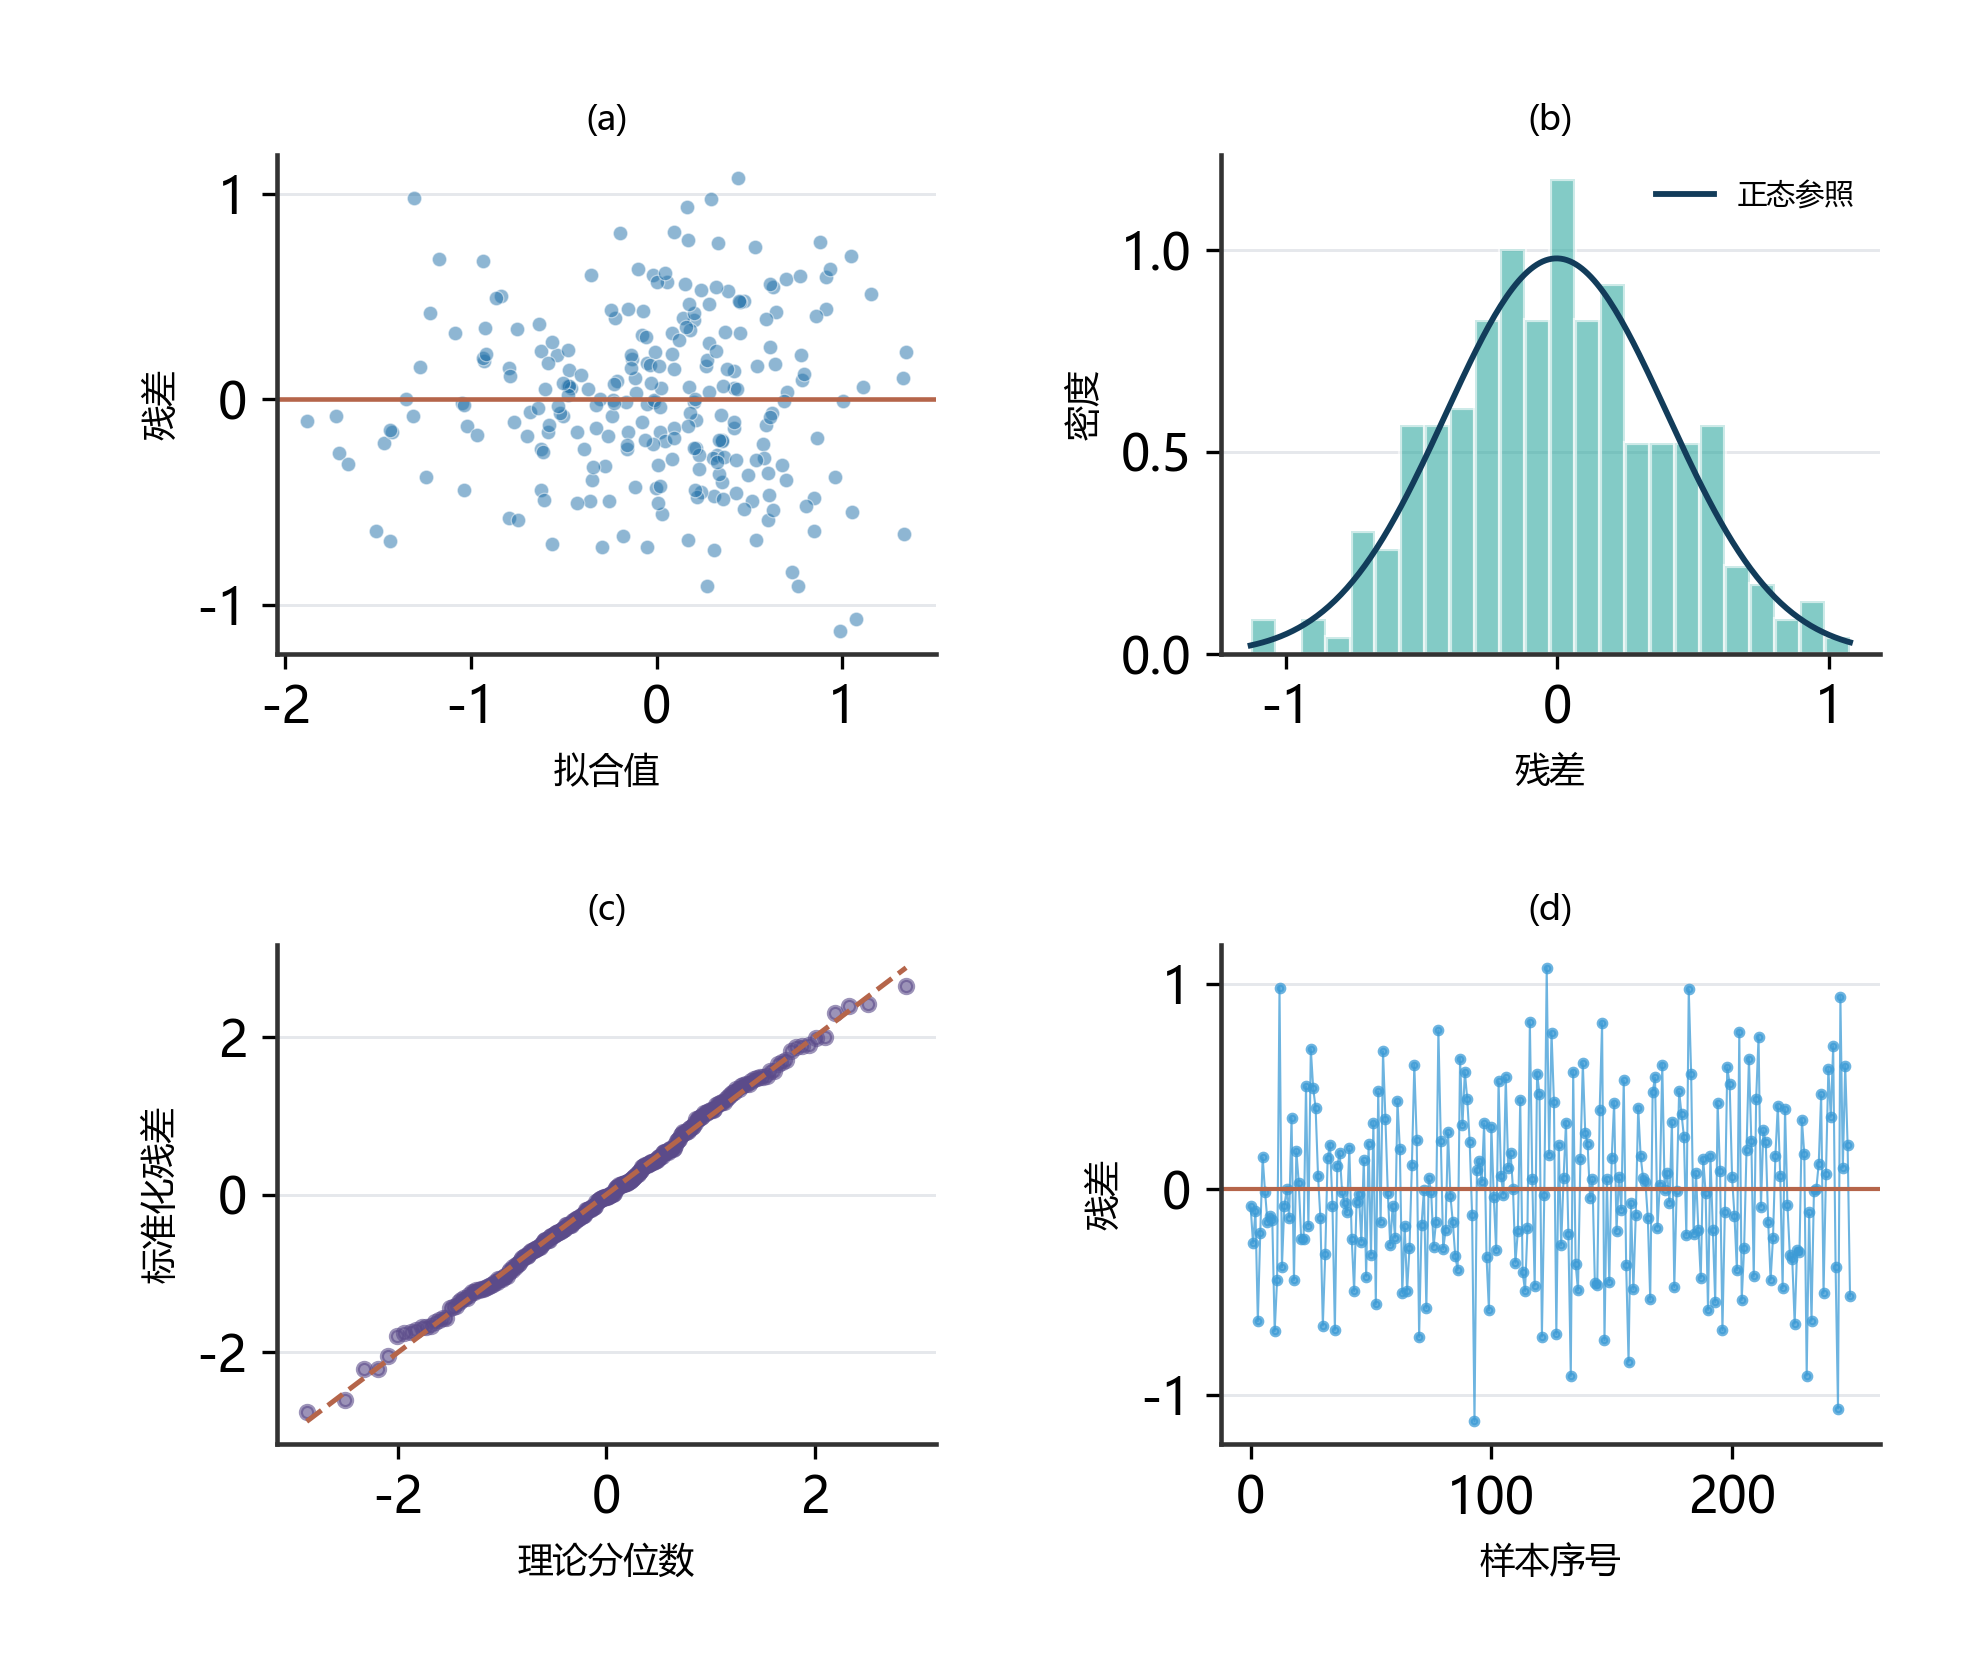
\includegraphics[width=0.62\textwidth]{figures/fig_q1_residual.png}
\caption{alcohol 项的残差四项诊断：残差散点、Q--Q 图、分布直方图与残差序列}
\label{fig:q1res}
\end{figure}

但这套诊断只在可预测的项上成立。推广到全部 50 项，只有 7 项的残差通过正态性检验，其 $p>0.05$；另有 26 项的偏度绝对值超过 1，全表共 189 个样本的标准化残差超过 3 倍标准差。原因与地板效应占比一致：当某一项有 40\% 以上的样本压在最低值时，残差必然是单侧长尾的。

\subsection{结果分析：失效原因与外部效度}

失效原因可以查清。图~\ref{fig:q1floor} 把地板效应占比与 $R^2$ 画在一起，两者的 Spearman 秩相关为 $-0.4009$，明显强于 Pearson 的 $-0.1158$，说明起作用的是单调关系而非线性关系：某项的左尾样本占比越高，模型越难学。这也是把 0.30 定为两段式触发阈值的依据。需要说明的是，两段式组的平均 $R^2$ 为 0.1823，低于非两段式组的 0.2310，即两段式并没有提升精度；它的价值在于把“是否感知”与“感知多强”分开表述，使 acetic、lactic 这类高地板效应占比项的结果可以解释。

\begin{figure}[htbp]
\centering
\begin{subfigure}[t]{0.48\textwidth}
\centering
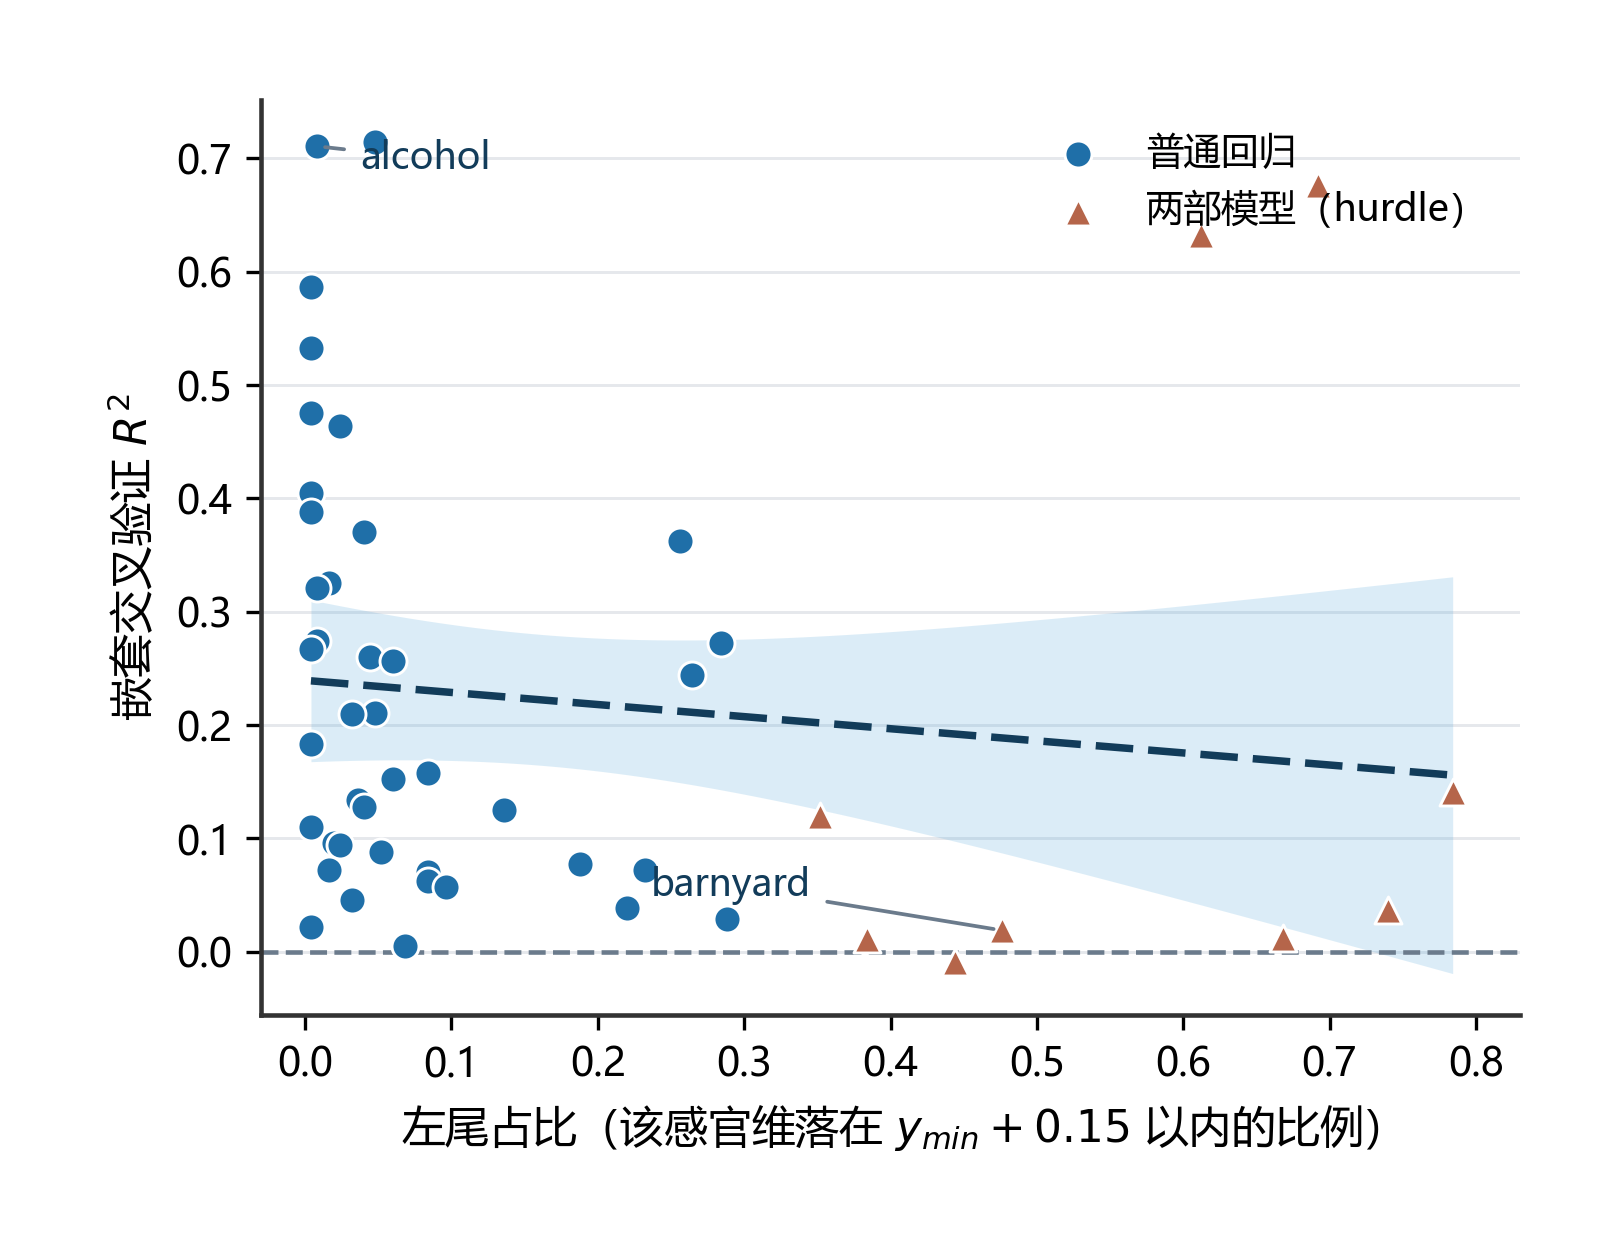
\includegraphics[width=\linewidth]{figures/fig_q1_floor_vs_r2.png}
\caption{左尾占比与 $R^2$ 的单调关系：左尾样本占比越高，模型越难学}
\label{fig:q1floor}
\end{subfigure}
\hfill
\begin{subfigure}[t]{0.48\textwidth}
\centering
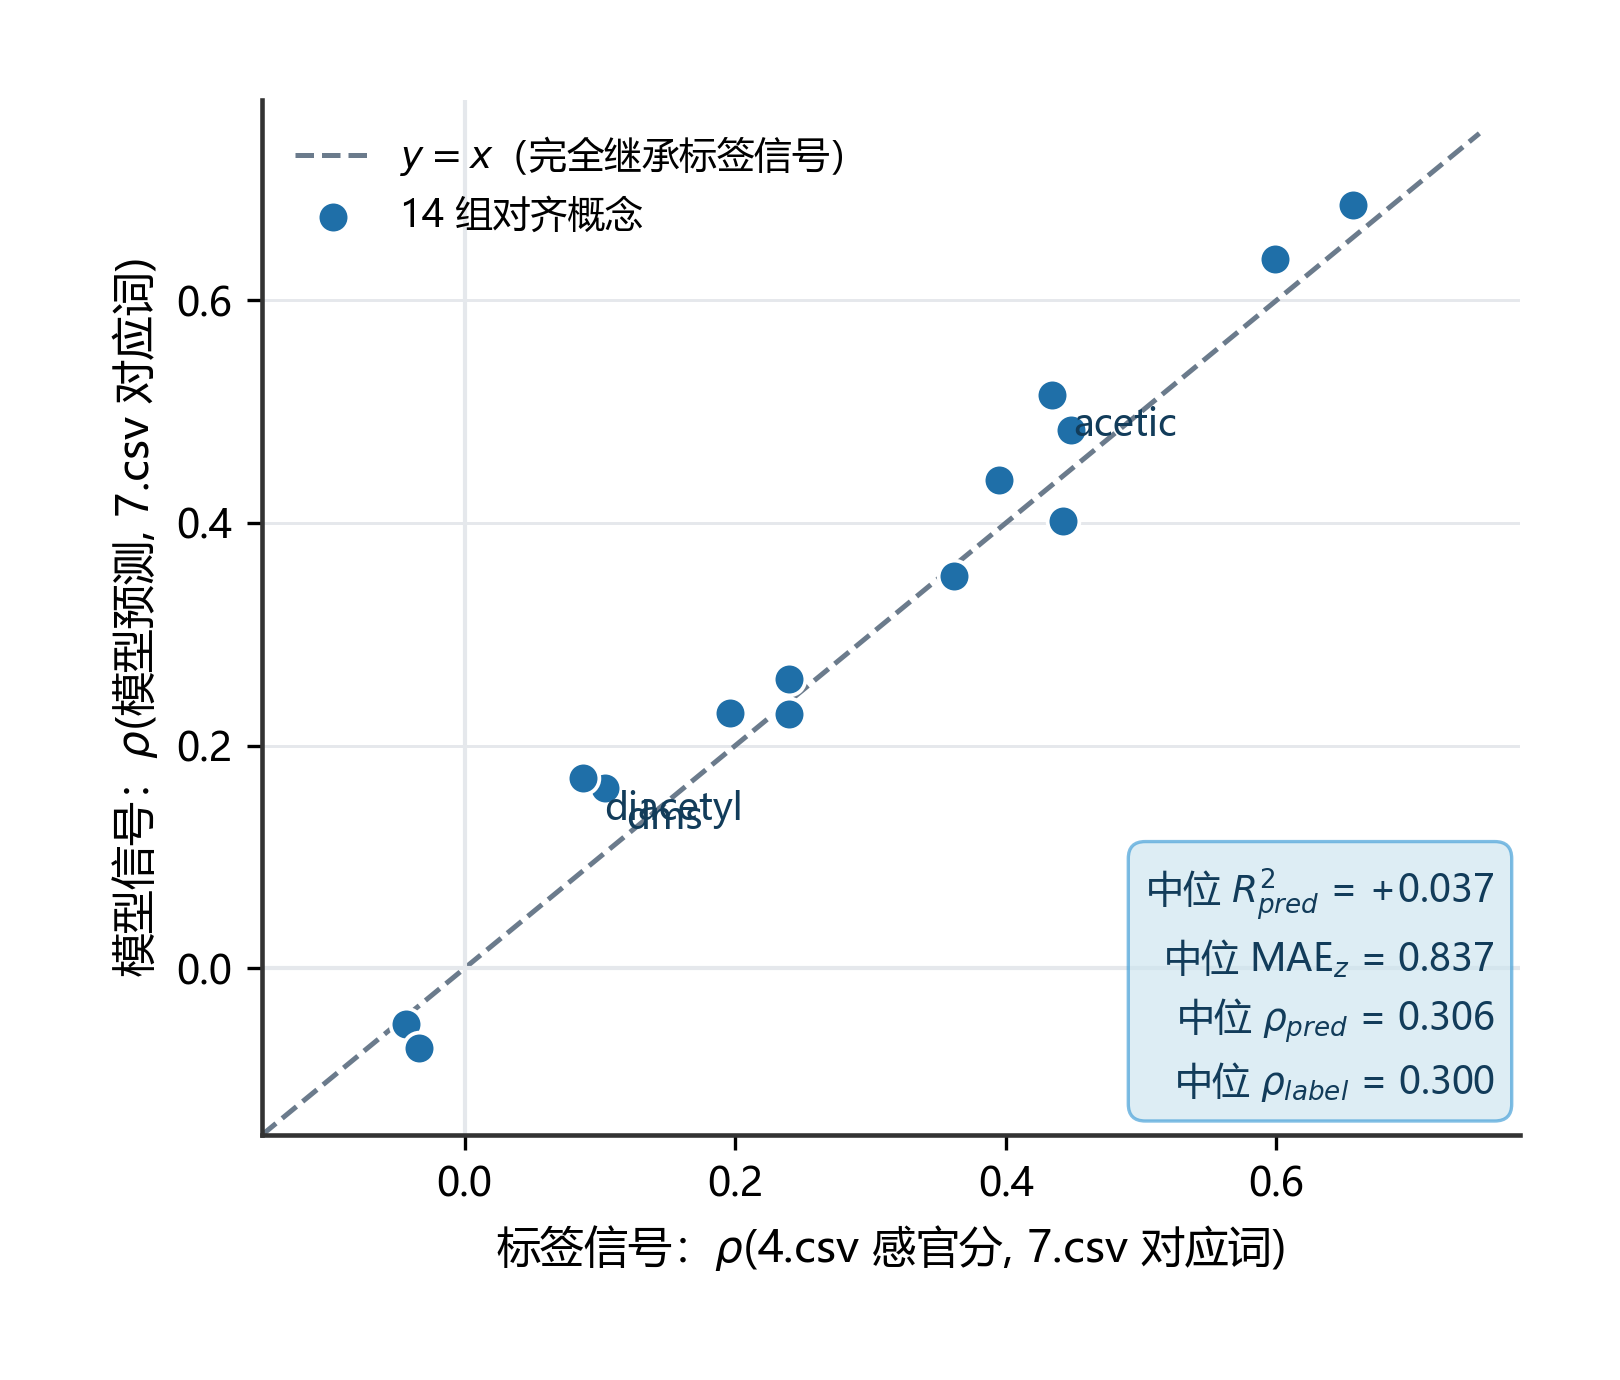
\includegraphics[width=\linewidth]{figures/fig_q1_external.png}
\caption{外部效度：模型预测与原始标签对附件7 的解释力对比，两线贴近对角线说明二者信息量相当}
\label{fig:q1ext}
\end{subfigure}
\caption{失效诊断与外部效度。左图为地板效应占比与 $R^2$ 的单调关系，是 0.30 触发阈值的依据；右图为模型预测与原始标签对附件7 的解释力对比}
\end{figure}

最后做外部效度检验。附件7 是一套独立的论坛评论描述符，与附件4 不同源。做法是在全部 250 个样本上用岭回归拟合"化学谱→附件4 单项"，再把这套拟合值与该单项在附件7 的对应词算秩相关，中位 0.3062；附件4 原始标签与附件7 的相关中位为 0.3005，两者几乎相同，见图~\ref{fig:q1ext}。

这一步用的是\textbf{全样本拟合}而非折外预测，因此这两个数应读作外部关联的\emph{上界}：它回答的是"化学谱能不能解释与论坛评论同向的感官差异"，不回答"模型泛化到新样本时还能不能"。之所以不换成折外预测，是因为附件7 与附件4 的语义对应只覆盖 14 个感官项（50 项中其余 36 项在论坛描述符里没有对应词），样本量不足以支撑逐项的折外检验。这说明模型确实学到了与真实品饮感受相关的信号，但没有比原始标签提供更多信息。跨附件 $R^2$ 中位仅 0.0372、z 尺度平均绝对误差 0.8368，也印证两套标签体系不能互相替代——附件7 只能作参照，不能当第二份训练数据。



\subsection{0--6 分级映射}

题面要求给出 0--6 分的评分。6.1 节已经说明附件4 只有中心化连续值，仿射搜索的残差落在 0.11 到 0.15、落不到整数格点，原始整数分不能精确还原。本节用\emph{先验分位映射}把连续预测转成等级：先在每一项内把强度换成百分位秩，再按给定的等级比例把秩切成 7 档
\begin{equation}
  g_{is}=\sum_{k=0}^{5}\mathbb{I}\left(r_{is}>C_{s,k}\right),\qquad
  C_{s,k}=\sum_{l=0}^{k}p_l,\qquad
  r_{is}=\frac{\operatorname{rank}\left(y_{is}\right)}{n},
\end{equation}
其中 $r_{is}\in(0,1]$ 为第 $s$ 项内第 $i$ 个样本的百分位秩，$p=(p_0,\dots,p_6)$ 为各等级的预期比例，$C_{s,k}$ 为累积切点。这里有一个必须讲清的度量口径。附件4 的原始 0--6 分值不可反解，因此不存在"真值切点"可以直接套到预测上——真值本身也只是一列连续强度。本文的做法是把真值与预测\emph{各自}映射到同一目标边际（即 $p$ 规定的等级比例），再比较两边落在同档的比例。这样度量的是\textbf{同一目标边际下的档位一致性}，衡量排序与分档的吻合程度，不是对面板真值的绝对分级精度。

由此有两点限制必须在读表~\ref{tab:q1grade} 时记住。其一，两条被映射后的分布在按构造上具有相同的等级比例，因此两者的总变差距离恒为 0，这个数不能作为"拟合好"的证据，本文也不报它。其二，分位映射会把预测的边际强行对齐到先验，若先验本身偏离真实边际，kappa 会同时偏高或偏低——这正是表~\ref{tab:q1grade} 要给出四组先验对照的原因：四组的 kappa 中位落在 0.3400 到 0.3812 之间、极差 0.041，说明结论对先验不敏感，但绝对水平依赖先验选择。

等级比例 $p$ 没法从数据反推。附件4 已按品评员做过 z-score 并按啤酒平均，这一步把原始 7 点量表上的厚零结构抹平了：实测每一列的最高频取值只占 1.8\%、恰等于列最小值的样本只占 0.88\%，因此“大量样品取最低档”这一结构\emph{在这份中心化数据上观察不到}。$p$ 只能取自 7 点感官量表的经验分布。

需要说明一处：表~\ref{tab:q1grade} 里零膨胀先验的 kappa（0.3400）并非四组中最高（均匀先验 0.3812、等频映射 0.3770、轻度零膨胀 0.3599）。本文仍以零膨胀为主方案，理由不是 kappa 最高，而是零膨胀的形状与 7 点量表的原始评分结构一致——感官打分中最低两档通常占比最大，这是量表本身的特性，不因本文数据经过中心化而改变；其余三组作为敏感性对照，用于界定“换先验会改变多少”。换言之，主方案按\emph{先验合理性}选定，kappa 的四组差异（极差 0.041）只用于说明该选择对结论的影响幅度，不用于反向挑选最高分。主方案取零膨胀分布 $p=(0.50,\allowbreak 0.18,\allowbreak 0.12,\allowbreak 0.09,\allowbreak 0.06,\allowbreak 0.035,\allowbreak 0.015)$；另设三组对照：均匀分布($p$ 全为 $1/7$)、轻度零膨胀 $p=(0.35,\allowbreak 0.20,\allowbreak 0.16,\allowbreak 0.13,\allowbreak 0.09,\allowbreak 0.05,\allowbreak 0.02)$、等频映射($p$ 全为 $1/7$ 且切点严格取该列的 6 个等分位点)。

\begin{table}[htbp]
\centering
\footnotesize
\caption{0--6 分数映射的四组设定与取整对照，取 50 项中位值}
\label{tab:q1grade}
\footnotesize
\setlength{\tabcolsep}{4.5pt}
\begin{tabular*}{\textwidth}{@{\extracolsep{\fill}}lccccc@{}}
\toprule
\textbf{映射方案} & \textbf{kappa} & \textbf{同档率} & \textbf{$\pm1$ 档} & \textbf{等级 MAE} & \textbf{压 0 占比} \\
\midrule
零膨胀分布（本文） & 0.3400 & 0.390 & 0.672 & 1.208 & -- \\
均匀分布 & 0.3812 & 0.216 & 0.538 & 1.690 & -- \\
轻度零膨胀 & 0.3599 & 0.298 & 0.630 & 1.356 & -- \\
等频映射 & 0.3770 & 0.216 & 0.530 & 1.694 & -- \\
\midrule
平移后直接取整（反例） & 0.1244 & 0.406 & -- & -- & 53.2\% \\
\bottomrule
\end{tabular*}
\end{table}

表~\ref{tab:q1grade} 的第一组结论是等级比例的影响有限：四组设定的加权 kappa 中位落在 0.3400 到 0.3812 之间，极差 0.041。换言之，改变等级比例只改变绝对水平，不改变哪些项可预测。这一点排除了“结论由比例挑选出来”的疑虑。

四组设定之间仍有一处实质差异，即精确同档率：零膨胀分布 0.376，其余三组只有 0.21 左右。原因在于附件4 的标签集中在中低档，而零膨胀比例把切点推向低档，预测与标签在低档更容易重合。这不等于精度更高——同档率只统计“落在同一档”的比例，不区分相邻档的错位，而 kappa 用二次权重、跨档越远罚得越重，因此本文以 kappa 为主要依据。

表~\ref{tab:q1grade} 最后一行是关键对照。若按“先平移到非负再四舍五入”这种看似自然的做法，中位 53.2\% 的样本被压到 0 分，加权 kappa 掉到 0.1244，与随机分档无异。值得注意的是这一行的精确同档率反而高达 0.406，甚至高于主方案——这正是同档率不能单独使用的证据：预测全部压在最低档，与同样集中于低档的标签大范围重合，同档率被“双方都取 0”抬起来。可见分级映射不是收尾步骤，而是问题一能否成立的前提。

50 项的 kappa 中位 0.3400、34 项超过 0.3、16 项超过 0.5；最优的 lactic 达 0.7414，最差的 overall 仅 0.1531。这与连续域的 $R^2$ 中位 0.1469 是同一件事的两种表述：化学谱对感官的解释力本身有限，分级只是把这种有限性摆到明面上。因此分级结果按项分层使用：kappa 高于 0.5 的可作评分参考，0.3 到 0.5 之间只宜作相对比较，低于 0.3 的不宜单独解读。此外附件4 没有 0--6 真值，本文报告的 kappa 与同档率都是同一映射内的往返一致性，衡量预测分与标签分落在同一档的比例，不是对感官面板真值的绝对精度。这条限制换模型也消除不了，只能如实标注。

%==============================================================================
% 七、问题二的模型建立与求解
%==============================================================================
\section{问题二：关键化合物的归因}

\subsection{建模思路}

问题二要求给出每个感官项最关键的三类化合物，并论证结果稳定、化学上讲得通。建模前须先排除两条看似可行的捷径。

第一条是直接采用附件8 的现成排序。该文件已提供 MDI 与 SHAP 两张化合物重要性表，取用最省力，但不适用：二者是全部 231 列对某一个综合目标的排序，并非对 50 个感官项分别排序；且重要性只说明模型在多大程度上用到了该列，不说明因果关系\cite{lundberg2017}。本文只把这两张表留作事后方向对照。

第二条是逐列计算重要性。231 个指标中有 219 个的方差膨胀因子大于 10，而相关系数绝对值超过 0.9 的只有 6 对，说明共线是一大片弱相关的累积而非少数几列重复。此时逐列打乱，被打乱的列会被同族其余列顶替，算出的重要性系统性偏小\cite{strobl2008}。

排除这两条之后，本问的技术路线分四步：先诊断附件2 的化合物网络能否直接用于分组；再用\emph{逐列置换重要性}配合 \emph{LightGBM} 完成候选排序；用\emph{自助重采样} 200 次量化稳定性；最后用\emph{气味活性值}作化学裁判。

\subsection{化合物网络的结构诊断}

题面要求以附件2 建立化合物共表达图。本文先按 $|\rho|\geq\tau$ 阈值化后取组合拉普拉斯 $L=D-A$，做特征分解并在前 $k$ 个特征向量上跑 \emph{Ng--Jordan--Weiss 谱聚类}($k=12$)，再计算模块内与模块间的平均 $|\rho|$。这张矩阵已与附件1 的 Spearman 相关逐格复核：231 个节点中 212 个可经附件8 的化学名—字段名对照表对应到本文的 231 维特征，44732 个可比对格子的中位绝对差为 $8.33\times10^{-17}$，说明矩阵本身没有读错。

按原设定做下去会得到“社区结构很弱”的结论。本文复查后认为这个判断不成立，原因分三层。

第一层是实现问题。谱聚类用纯随机初始化时，在这张图上收敛到退化解——231 个节点里有 79\%(183 个)被并进同一个“模块”。一个吞掉八成节点的划分，模块内与模块间自然拉不开差距，1.56 这个数字度量的是退化程度，不是图的结构。

第二层是方法问题。换成标准 Ng--Jordan--Weiss 所用的归一化拉普拉斯 $L_{\mathrm{sym}}=I-D^{-1/2}AD^{-1/2}$ 并加上 k-means++ 重启后，退化明显缓解，最大模块占比由 0.79 降到 0.38，但该划分的模块度仍只有 $-0.0034$。可见问题不在初始化，而在谱聚类本身：它以固定簇数 $k=12$ 切分，在密度 14.7\% 的稠密图上，前 12 个特征向量并不携带社区信息。

第三层才是图本身的结论。改用直接优化模块度的 \emph{Louvain 算法}，得 9 个社区、$Q=0.3229$，而 50 次度保持随机图的 95 分位为 0.2501，超出 0.0728；七个阈值下 $Q$ 均高于零分布，可见社区结构真实存在。三种聚类方式的定量对照见表~\ref{tab:q2graph}，模块度检验与模块内外相关性的对比见图~\ref{fig:q2graph}。

\begin{table}[htbp]
\centering
\footnotesize
\setlength{\tabcolsep}{3.5pt}
\caption{化合物网络的三种聚类方式对照。$\tau$ 为边阈值，$Q$ 为模块度}
\label{tab:q2graph}
\begin{tabular*}{\textwidth}{@{\extracolsep{\fill}}cccccc@{}}
\toprule
$\tau$ & \textbf{边数} & \textbf{原谱聚类：最大模块 / 内间比} & \textbf{归一化 $L$：最大模块 / $Q$} & \textbf{Louvain $Q$} & \textbf{零分布 95\%} \\
\midrule
0.10 & 15855 & 0.88 / 1.69 & 0.19 / $-0.0039$ & 0.0822 & 0.0538 \\
0.15 & 11642 & 0.80 / 1.58 & 0.17 / $-0.0039$ & 0.1359 & 0.0943 \\
0.20 & 8323  & 0.79 / 1.50 & 0.32 / $-0.0036$ & 0.1872 & 0.1397 \\
0.25 & 5739  & 0.60 / 1.50 & 0.28 / $-0.0036$ & 0.2474 & 0.1900 \\
0.30 & 3918  & 0.79 / 1.56 & 0.38 / $-0.0034$ & 0.3229 & 0.2501 \\
0.40 & 1660  & 0.38 / 1.42 & 0.47 / $-0.0032$ & 0.4831 & 0.3911 \\
0.50 & 645   & 0.58 / 1.67 & 0.61 / $-0.0026$ & 0.6513 & 0.5453 \\
\bottomrule
\end{tabular*}
\end{table}

\begin{figure}[htbp]
\centering
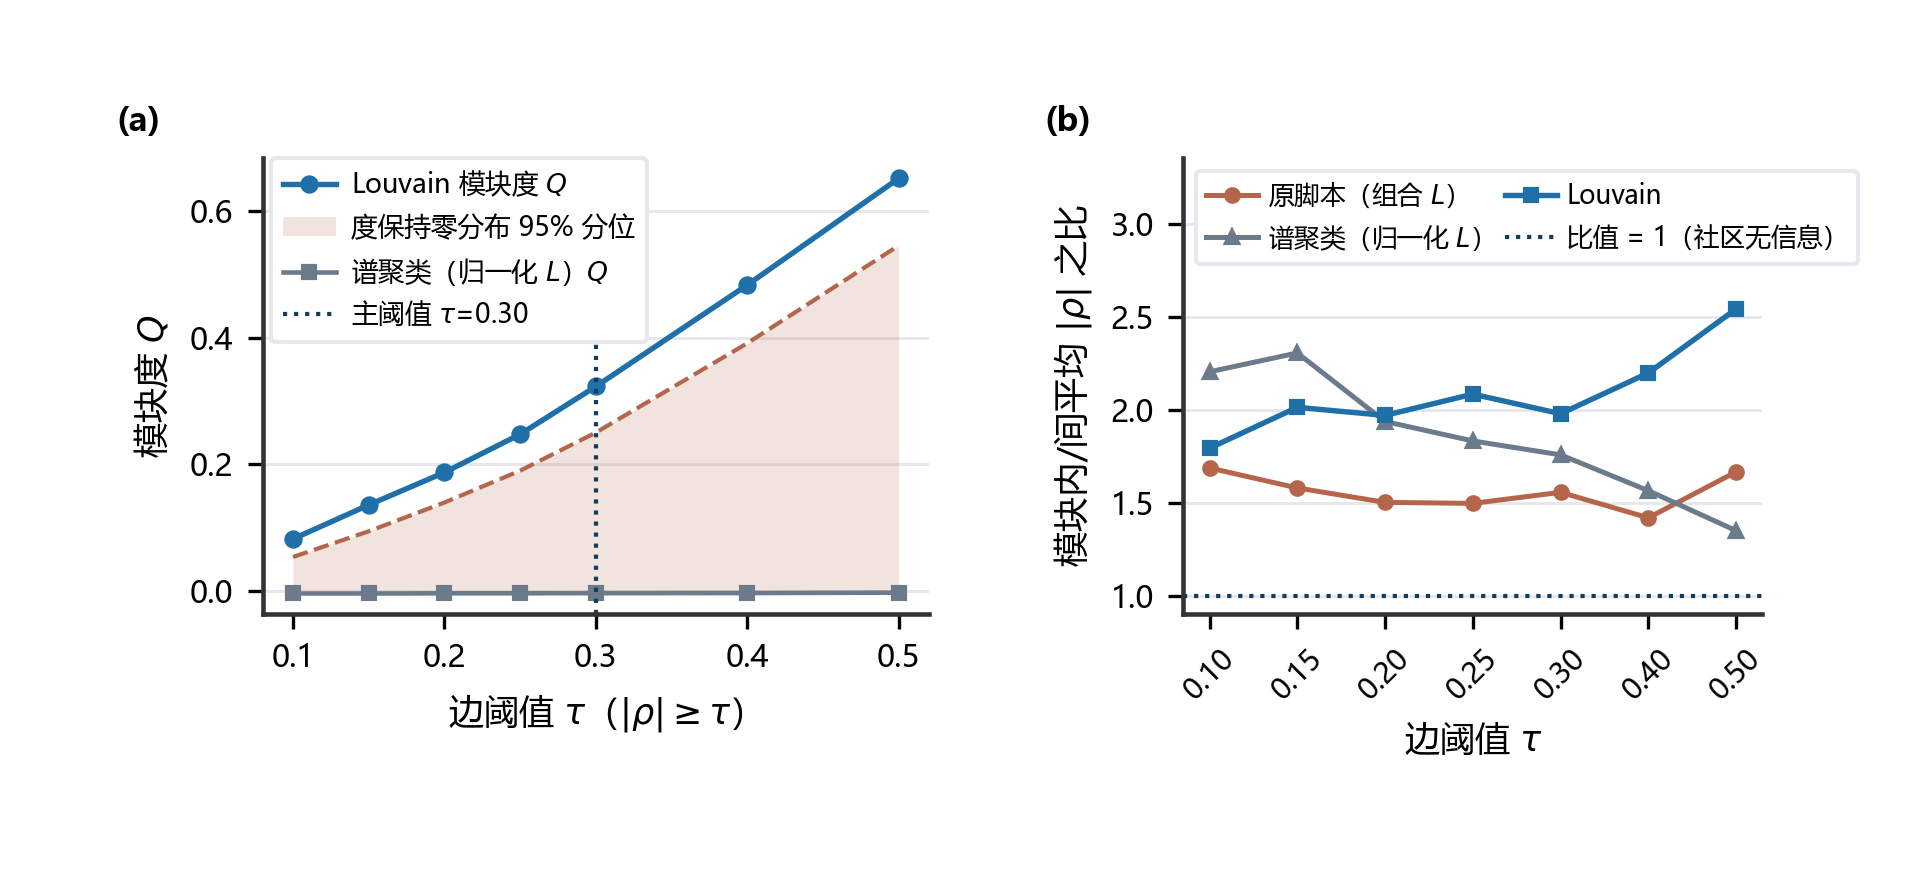
\includegraphics[width=0.79\textwidth]{figures/fig_q2_graph.png}
\caption{化合物网络的结构诊断。左图为 Louvain 模块度与度保持零分布，右图为三种聚类方式的模块内外 $|\rho|$ 对比}
\label{fig:q2graph}
\end{figure}

但这些社区不能直接用来做归因。把 Louvain 的 9 个社区与附件8 的化学来源分组对照，二者的调整兰德指数仅 0.0838、调整互信息仅 0.1109；反过来把化学族直接当作社区划分，模块度只有 0.0533。换言之，数据给出的社区与化合物来源几乎无关。同时 9 个社区覆盖 231 个节点、最大社区占 25\%，每个“模块”约 25 个化合物——用它做 Top-3 归因，等于先把 25 个化合物捆成一个不可拆的组，无法回答“哪 3 个最关键”这一题意。

因此本文的取舍是：附件2 的图用于结构诊断与特征预筛，归因的分组单位取附件8 的化学来源标注。三条理由都可量化：社区在统计上真实，$Q$ 高于零分布；在化学上不可解释，ARI 仅 0.0838；在粒度上不可用，约 25 个一组。

归因所用的分组来自附件8：231 个特征全部落在 7 族内，酵母代谢产物 78 个、酒花来源 77 个、其他 25 个（含 5 个派生总量）、香料陈化 23 个、麦芽 21 个、野生菌群 6 个、内标 1 个。这一划分有化学依据，且与前述共线结构相容——同族的弱相关累积正是共线的来源。

\subsection{逐列置换重要性与入选频率模型}

置换重要性的定义是“打乱某一列后预测性能掉多少”。逐列打乱有一个已知的缺陷：被打乱的列可以由同族的其他列顶上，掉幅被系统性低估\cite{strobl2008}。整族同时打乱可以避开这个偏差，但整族只给出 7 个族级数值，无法直接落成化合物排名——族内数十列共享同一个族级数值，要拆到单列只能按人为比例摊派，而摊派方式本身决定排名。本问要交付的是单个化合物的 Top-3，因此取逐列置换，族标签只用于汇报分组归属，不用于整组打乱。

本文对 50 个感官项分别建立 \emph{LightGBM 回归器}，在第 $b$ 次自助重采样的袋外样本上先算逐列置换重要性
\begin{equation}
  \Delta^{(b)}_{j}=R^{2}\left(\text{原样}\right)-R^{2}\left(\text{打乱第 }j\text{ 列}\right),
\end{equation}
再统计它进入前 10 名的频率
\begin{equation}
  \pi_{j}=\frac{1}{B}\sum_{b=1}^{B}\mathbf{1}\left[j\in\mathrm{Top10}\left(\Delta^{(b)}\right)\right],
  \qquad B=200,
\end{equation}
得到的是\emph{入选频率}而非单次重要性：单次 $\Delta^{(b)}_{j}$ 的噪声大到会反复变号，而 $\pi_j\in[0,1]$ 表示该列在 200 次重采样中稳居前 10 的比率，可以直接横向比较。第 $s$ 个感官项的 Top-3 取 $\pi_j$ 最大的三列构成 $\mathcal{T}_s$。由于实现上并未整族打乱，Top-3 应理解为模型相关性候选，不宜解释为独立的因果效应。

阈值由稳定选择的有限样本界反解。该界为 $\mathbb{E}[V]\le q_{\mathrm{sel}}^{2}/\left((2\pi_{\mathrm{thr}}-1)p\right)$，其中 $V$ 为误选变量数、$q_{\mathrm{sel}}$ 为基础选择程序每次选出的变量数、$p$ 为候选变量数。本文取 $q=1$、$p=231$，得
\begin{equation}
  \pi_{\mathrm{thr}}=\frac{1+q/p}{2}=0.5022 .
\end{equation}
这里 $q=1$ 的含义是“允许期望误选 1 个变量”，属操作性标准，\emph{不构成} 0.05 水平上的错误发现率控制——若严格按界中 $q_{\mathrm{sel}}$ 的原义取基础程序的选出数 10，同一式给出 0.7165，本文未采用。因此下文只称 $\pi_{\mathrm{thr}}$ 为入选频率阈值，不主张理论保证的错误发现率控制。

化学合理性用\emph{气味活性值}判断。对化合物 $j$ 与感官项 $i$，定义
\begin{equation}
  O_{ij}=\frac{c_{ij}}{T_j},
\end{equation}
$T_j$ 取自附件8 的香气阈值表，按单位分域处理(30 个阈值在 $\log_{10}$ 域、13 个在线性域，分别与浓度同域相除，不混用)。$O_{ij}>1$ 表示该化合物在样本中的浓度已超过其香气阈值，具备被感知的物质基础。据此把 150 条 Top-3 记录分为四档，判据只依赖阈值能否计算，不叠加显著性——显著性由 $\pi_{\mathrm{thr}}$ 单独把关：A 档阈值可算且 $O_{ij}\geq1$，浓度已超香气阈值；B 档阈值可算且 $0.5\leq O_{ij}<1$，接近阈值；C 档阈值可算但 $O_{ij}<0.5$，远低于阈值；N 档阈值缺失（表中无该化合物，或有行但阈值为 NA），OAV 不可算。

跨模型的稳定性用 \emph{Jaccard 系数}度量
\begin{equation}
  J\left(\mathcal{T}_s^{\,A},\mathcal{T}_s^{\,B}\right)
  =\frac{\left|\mathcal{T}_s^{\,A}\cap\mathcal{T}_s^{\,B}\right|}{\left|\mathcal{T}_s^{\,A}\cup\mathcal{T}_s^{\,B}\right|},
\end{equation}
取 LightGBM、ExtraTrees、岭回归三模型 Top-10 集合两两比较。

\subsection{模型求解}

\noindent\textbf{置换的执行方式}\quad 每次自助重采样有放回地抽 250 个样本，在抽中的样本上训练 LightGBM，在未被抽中的袋外样本上按列逐次打乱并重算 $R^{2}$，一次重采样内 231 列各打乱一遍。231 列全部参与置换与前 10 名的竞争：其中 19 列属理化指标、派生总量与内标，它们照常打乱、不进 Top-3 候选池，但保留在模型里作背景变量——若先把它们剔除，剩下的列会吸收它们的解释力，重要性被虚高。报告 Top-3 时只从香气候选池（212 列）内取，实测 150 条记录中非香气成分 0 条。

\noindent\textbf{重采样次数与阈值}\quad 50 个感官项各做 $B=200$ 次自助重采样。题面建议的下限是 30 次，取 200 是为了让 $\pi$ 收敛：逐次增量在 200 次后已落进标准误带内（自助标准误均值 0.0096、95 分位 0.0275），继续加次数不改变判定。阈值按 7.3 节的界取 $q=1$、$p=231$，得 $\pi_{\mathrm{thr}}=0.5022$，50 项共用同一阈值、不按项调参。实测 231 个特征中有 46 个在某个感官项上曾越过该阈值。

\noindent\textbf{化学合理性的判定}\quad 统计显著只说明模型依赖该列，不说明它真是香气来源。因此对每条 Top-3 记录再算气味活性值，即浓度除以该化合物的香气阈值。阈值来源分两类：30 个化合物在附件8 中以 $\log_{10}$ 给出，13 个以线性浓度给出，共 43 个可算 OAV，其中属于香气化合物的 35 个。按 OAV 与统计显著性组合成 A、B、C、N 四档：A 档显著且 $\mathrm{OAV}>1$，B 档显著但 OAV 仅在阈值附近，C 档显著而浓度远低于阈值，N 档因阈值表缺项无法判断。

\noindent\textbf{跨模型的一致性检验}\quad 名单是否只在 LightGBM 下成立，需要换模型重跑。做法是在同一份分层 $70/30$ 划分上训练 LightGBM、随机森林与岭回归三个模型，三者共用同一个 $30\%$ 评估集，各自给出 Top-10 后两两算 Jaccard。中位 Jaccard 为 0.0974，最差一对仅 0.0175，LightGBM 与岭回归之间为 0.0526。这个结果说明名单高度依赖模型族，本文在 7.5 节把它作为短板如实报告，而不是用单一模型的排名充当结论。

\noindent\textbf{计算量}\quad 主体开销是 $50$ 项 $\times 200$ 次重采样 $\times$ 7 组的置换计算，折算约 7 万次模型前向计算；跨模型一致性部分额外训练 3 个模型。全部流程在单机串行执行，耗时 363.5 秒。

图~\ref{fig:q2conv} 与图~\ref{fig:q2jac} 分别给出两处稳定性的检验：左图是 $\pi$ 在重采样过程中的收敛轨迹，200 次之后逐次增量已落入标准误带内(自助标准误均值 0.0096、95 分位 0.0275)，说明继续加大 $B$ 不会改变显著性判定；右图是跨模型 Jaccard 的分布。

\begin{figure}[htbp]
\centering
\begin{subfigure}[t]{0.48\textwidth}
\centering
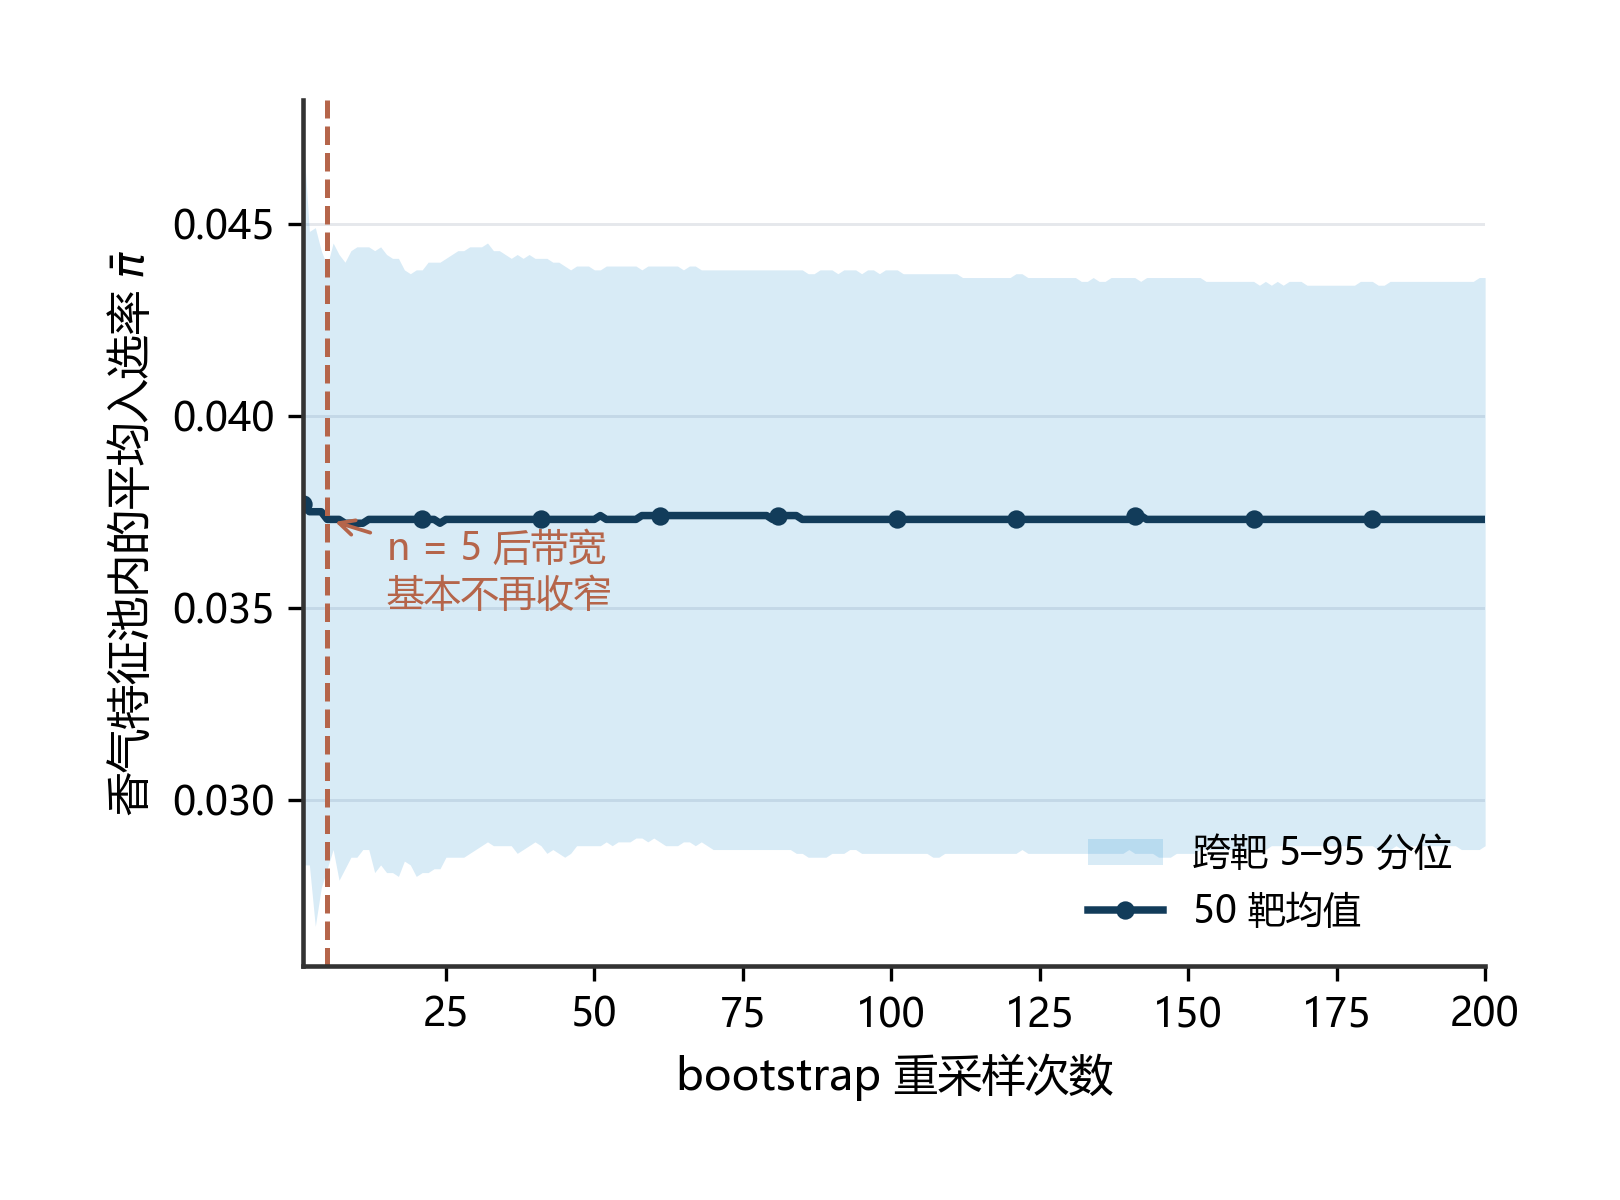
\includegraphics[width=\linewidth]{figures/fig_q2_convergence.png}
\caption{$\pi$ 的自助收敛}
\label{fig:q2conv}
\end{subfigure}
\hfill
\begin{subfigure}[t]{0.48\textwidth}
\centering
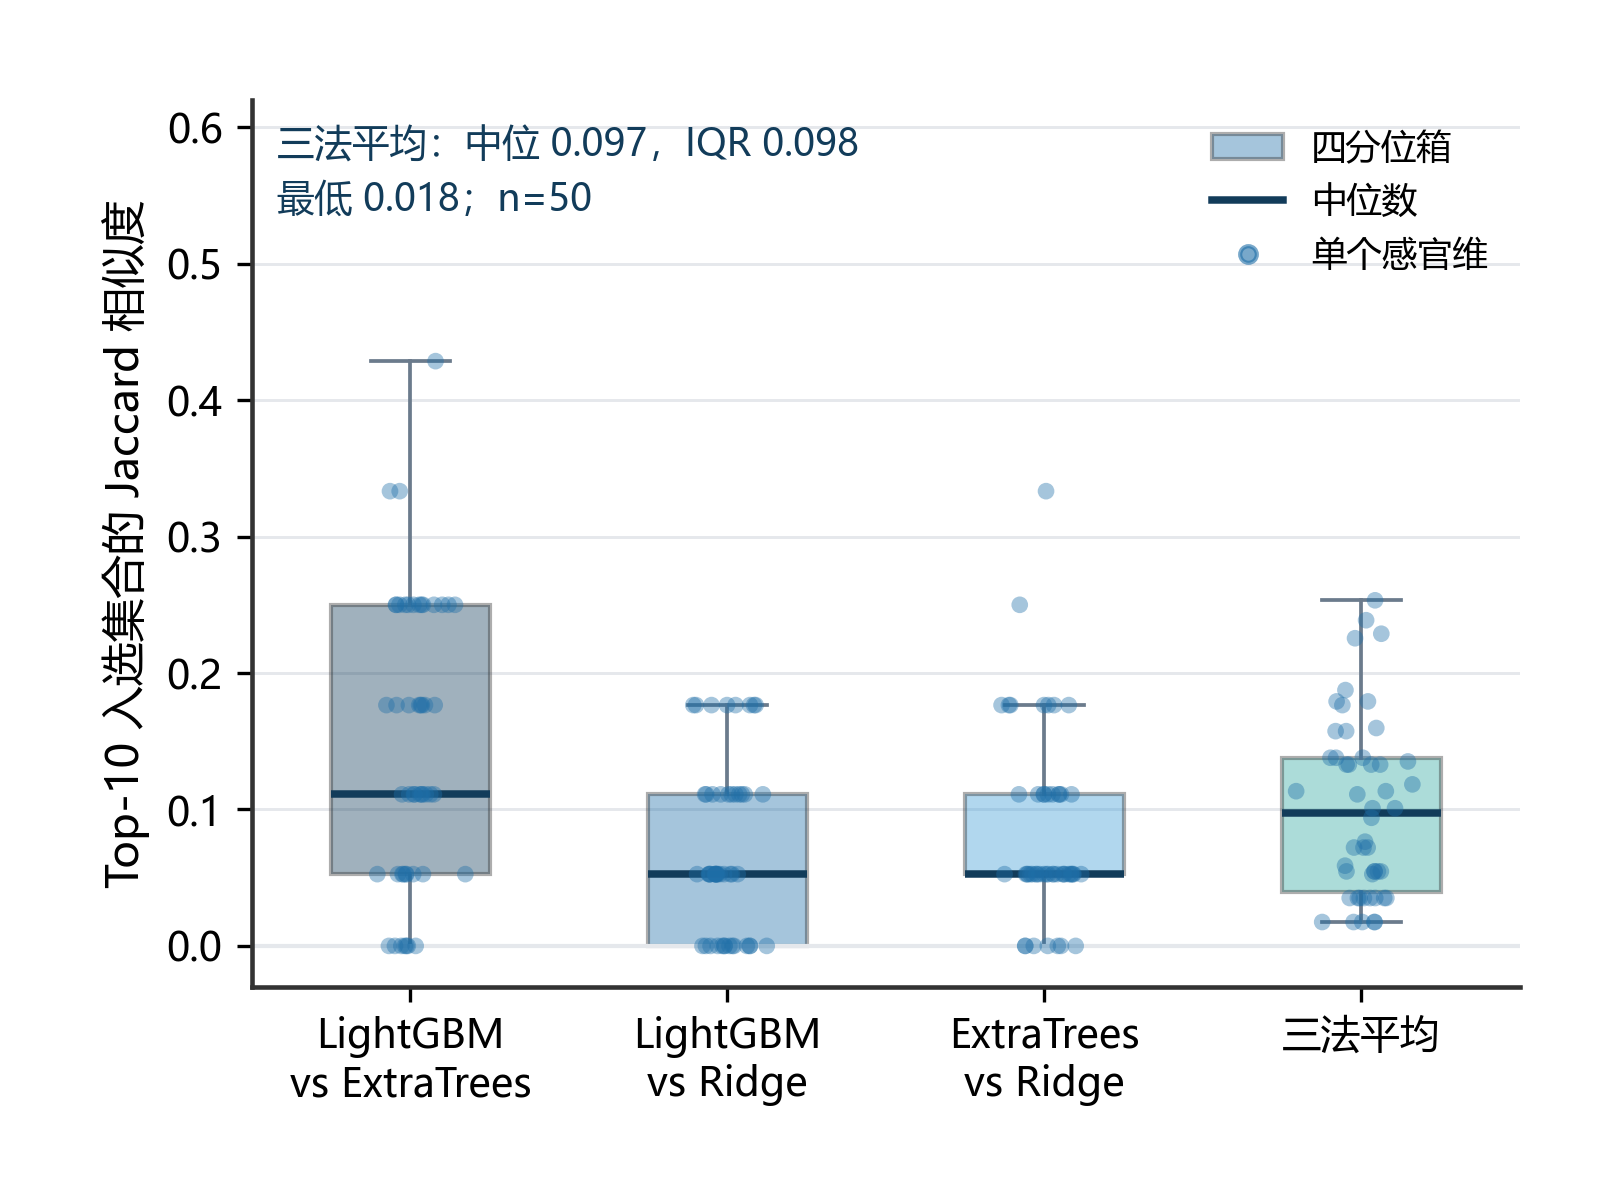
\includegraphics[width=\linewidth]{figures/fig_q2_jaccard.png}
\caption{跨模型 Jaccard 分布}
\label{fig:q2jac}
\end{subfigure}
\caption{稳定性的两项检验。左图为重采样 200 次后增量进入标准误带，说明次数够用；右图为跨模型 Jaccard 分布，中位仅 0.0974，说明名单高度依赖模型族}
\end{figure}

\subsection{结果分析}

231 个化合物中有 46 个在至少一个感官项上超过阈值。150 条 Top-3 记录按阈值能否计算分两条线：67 条有阈值可算 OAV，其中 62 条同时通过 $\pi$ 显著性阈值（$\pi_{\mathrm{thr}}=0.5022$），另 5 条只过 OAV 而不过 $\pi$。四档的分布见表~\ref{tab:q2grade}：A 档 19 条、B 档 8 条、C 档 40 条、N 档 83 条，A+B+C 恰为 67。Top-3 中没有任何理化指标、派生量或内标混入，说明分类规则在前置环节收住了。

\begin{table}[htbp]
\centering
\footnotesize
\caption{问题二 Top-3 记录的证据分级}
\label{tab:q2grade}
\begin{tabular*}{\textwidth}{@{\extracolsep{\fill}}clc}
\toprule
\textbf{档位} & \textbf{判定条件} & \textbf{记录数} \\
\midrule
A & 阈值可算且 $\mathrm{OAV}\geq1$，化学上确可被感知 & 19 \\
B & 阈值可算且 $0.5\leq\mathrm{OAV}<1$，接近阈值 & 8 \\
C & 阈值可算但 $\mathrm{OAV}<0.5$，远离阈值 & 40 \\
N & 阈值缺失（表中无该行，或有行但阈值为 NA），OAV 不可算 & 83 \\
\bottomrule
\end{tabular*}
\end{table}

全部 50 项的 Top-3 名单按能否做化学裁判拆成两张表：表~\ref{tab:q2top3a} 是 A/B 档（至少一个化合物阈值可算且可被闻到），表~\ref{tab:q2top3b} 是 C/N 档（阈值缺失或 OAV 远低于阈值）。表中 $\pi$ 为逐列置换的入选频率，只在同一感官项内可比；末位字母为证据等级，括号内为 OAV 中位数。可以看到 50 项里有 31 项不存在 A 档记录——这不是遗漏，而是阈值表覆盖率不足的直接后果：261 行阈值里只有 43 行有数值，其余留空，注释里本文不把它们称为关键香气化合物。

\begingroup
\scriptsize
\setlength{\tabcolsep}{3.5pt}
\renewcommand{\arraystretch}{1.12}
\begin{longtable}{@{}>{\raggedright\arraybackslash}p{2.7cm}>{\raggedright\arraybackslash}p{4.1cm}>{\raggedright\arraybackslash}p{4.1cm}>{\raggedright\arraybackslash}p{4.1cm}@{}}
\caption{A/B 档：可用阈值做化学裁判的感官项 Top-3。每格第一行为化合物名，第二行为入选频率 $\pi$、证据等级与 OAV 中位数（$>1$ 表示浓度已超其香气阈值）}
\label{tab:q2top3a}\\
\toprule
\textbf{感官项} & \textbf{Top-1} & \textbf{Top-2} & \textbf{Top-3} \\
\midrule
\endfirsthead
\toprule
\textbf{感官项} & \textbf{Top-1} & \textbf{Top-2} & \textbf{Top-3} \\
\midrule
\multicolumn{4}{r@{}}{\footnotesize\itshape 续表~\ref{tab:q2top3a}}\\
\endhead
\bottomrule
\endlastfoot
A\_malt\_cara & octyl\_acetate\newline 0.35C (0.0) & acetic\_acid.\allowbreak g.\allowbreak L.\allowbreak \newline 0.34A (1.2) & furfural\newline 0.32C (0.0) \\
A\_hops\_all & DMS\newline 0.74A (1.4) & ethyl\_octanoate\newline 0.65B (0.7) & X2.\allowbreak 3.\allowbreak dihydro.\allowbreak farnesol\newline 0.34N \\
A\_hops\_tropical & isopentyl.\allowbreak butanoate\newline 0.68N & DMS\newline 0.49A (1.4) & n.\allowbreak hexanol\newline 0.36N \\
A\_hops\_noble & ethyl\_octanoate\newline 0.81B (0.7) & ethyl\_decanoate\newline 0.48C (0.1) & X2.\allowbreak acetylfuran\newline 0.40N \\
A\_esters\_ethac & phenethyl\_alcohol\newline 0.46C (0.2) & ethyl.\allowbreak tetradecanoate\newline 0.43N & ethyl\_acetate\newline 0.41A (1.2) \\
A\_esters\_isoaa & n.\allowbreak hexanol\newline 0.90N & isopentyl\_acetate\newline 0.83A (3.6) & ethyl\_decanoate\newline 0.46C (0.1) \\
F\_hops\_all & ethyl\_octanoate\newline 0.89B (0.7) & cis.\allowbreak dihydro.\allowbreak beta.\allowbreak terpineol\newline 0.68N & DMS\newline 0.52A (1.4) \\
F\_hops\_tropical & n.\allowbreak hexanol\newline 0.56N & nerol.\allowbreak oxide\newline 0.47N & DMS\newline 0.38A (1.4) \\
F\_hops\_noble & ethyl\_octanoate\newline 0.88B (0.7) & citronellol\newline 0.34A (8.8) & nerol.\allowbreak oxide\newline 0.29N \\
F\_esters\_all & n.\allowbreak hexanol\newline 0.67N & ethyl\_acetate\newline 0.66A (1.2) & acetaldehyde\newline 0.65C (0.1) \\
F\_esters\_ethac & ethyl\_acetate\newline 0.81A (1.2) & acetaldehyde\newline 0.47C (0.1) & Z.\allowbreak Z.\allowbreak geranyl.\allowbreak linalool\newline 0.43N \\
F\_esters\_isoaa & isopentyl\_acetate\newline 0.56A (3.6) & ethyl\_decanoate\newline 0.40C (0.1) & delta.\allowbreak terpinyl.\allowbreak acetate\newline 0.34N \\
F\_esters\_fruity & X1.\allowbreak 10.\allowbreak di.\allowbreak epi.\allowbreak cubenol\newline 0.59N & X.\allowbreak E.\allowbreak .\allowbreak alpha.\allowbreak ionone\newline 0.47N & acetic\_acid.\allowbreak g.\allowbreak L.\allowbreak \newline 0.35A (1.2) \\
acidity & lactic\_acid.\allowbreak mg.\allowbreak L.\allowbreak \newline 0.95C (0.3) & ethyl.\allowbreak phenylacetate\newline 0.73N & acetic\_acid.\allowbreak g.\allowbreak L.\allowbreak \newline 0.57A (1.2) \\
bitternes & ethyl\_octanoate\newline 0.94B (0.7) & butyl.\allowbreak acetate\newline 0.69N & ethyl\_decanoate\newline 0.57C (0.1) \\
orange & terpinen.\allowbreak 4.\allowbreak ol\newline 0.78N & geraniol\newline 0.69A (4.4) & ethyl.\allowbreak .\allowbreak E.\allowbreak .\allowbreak linalool\newline 0.57N \\
coriander & camphor\newline 0.86N & geraniol\newline 0.57A (4.4) & ethyl.\allowbreak .\allowbreak E.\allowbreak .\allowbreak linalool\newline 0.56N \\
acetic & lactic\_acid.\allowbreak mg.\allowbreak L.\allowbreak \newline 0.90C (0.3) & ethyl\_isovalerate\newline 0.69C (0.1) & acetic\_acid.\allowbreak g.\allowbreak L.\allowbreak \newline 0.65A (1.2) \\
alcohol & ethyl\_octanoate\newline 0.70B (0.7) & acetaldehyde\newline 0.53C (0.1) & ethyl\_acetate\newline 0.45A (1.2) \\
aftertaste & ethyl\_isovalerate\newline 0.68C (0.1) & acetaldehyde\newline 0.62C (0.1) & ethyl\_octanoate\newline 0.55B (0.7) \\
co2 & ethyl\_octanoate\newline 0.79B (0.7) & nerol\newline 0.69N & ethyl\_hexanoate\newline 0.41A (1.0) \\
overall & X2.\allowbreak ethyl.\allowbreak 1.\allowbreak hexanol\newline 0.47N & cis.\allowbreak linalool.\allowbreak oxide\newline 0.34N & ethyl\_acetate\newline 0.32A (1.2) \\
\end{longtable}
\endgroup



表~\ref{tab:q2top3a} 是被判为 A 档或 B 档的全部感官项——即至少有一个 Top-3 化合物既能算 OAV、又能被闻到。这一组的化学解释可直接给出：$\texttt{A\_malt\_cara}$ 的乙酸与焦糖麦芽香对应美拉德反应产物，$\texttt{A\_hops\_all}$ 的 DMS 与 $\texttt{F\_hops\_all}$ 的辛酸乙酯分别是酒花硫味与果香的主体，$\texttt{lactic}$/$\texttt{acetic}$ 直接对应两种有机酸。

\begingroup
\scriptsize
\setlength{\tabcolsep}{3.5pt}
\renewcommand{\arraystretch}{1.12}
\begin{longtable}{@{}>{\raggedright\arraybackslash}p{2.7cm}>{\raggedright\arraybackslash}p{4.1cm}>{\raggedright\arraybackslash}p{4.1cm}>{\raggedright\arraybackslash}p{4.1cm}@{}}
\caption{C/N 档：阈值缺失或 OAV 远低于阈值的感官项 Top-3。这些记录只作统计候选，不构成关键化合物结论}
\label{tab:q2top3b}\\
\toprule
\textbf{感官项} & \textbf{Top-1} & \textbf{Top-2} & \textbf{Top-3} \\
\midrule
\endfirsthead
\toprule
\textbf{感官项} & \textbf{Top-1} & \textbf{Top-2} & \textbf{Top-3} \\
\midrule
\multicolumn{4}{r@{}}{\footnotesize\itshape 续表~\ref{tab:q2top3b}}\\
\endhead
\bottomrule
\endlastfoot
A\_malt\_all & X2.\allowbreak acetylfuran\newline 0.35N & octyl\_acetate\newline 0.34C (0.0) & X.\allowbreak E.\allowbreak .\allowbreak alpha.\allowbreak ionone\newline 0.26N \\
A\_malt\_grain & X5.\allowbreak methylfurfural\newline 0.51N & terpinen.\allowbreak 4.\allowbreak ol\newline 0.33N & Z.\allowbreak nerolidol\newline 0.32C (0.0) \\
A\_malt\_bread & X2.\allowbreak acetylpyrrole\newline 0.34N & alpha.\allowbreak humulene\newline 0.30C (0.0) & ethyl.\allowbreak tiglate\newline 0.26N \\
A\_malt\_burn & methylpyrazine\newline 0.46C (0.0) & X2.\allowbreak acetylpyrrole\newline 0.23N & ethyl.\allowbreak furoate\newline 0.20N \\
A\_hops\_citrus & isopropyl.\allowbreak tetradecanoate\newline 0.27N & E.\allowbreak caryophyllene\newline 0.26C (0.0) & y.\allowbreak methyl.\allowbreak 1.\allowbreak octanol\newline 0.25N \\
A\_hops\_woody & alloaromadendrene.\allowbreak epoxide\newline 0.61N & X2Z.\allowbreak 6Z.\allowbreak farnesol\newline 0.34N & X1.\allowbreak octen.\allowbreak 3.\allowbreak ol\newline 0.34N \\
A\_esters\_all & n.\allowbreak hexanol\newline 0.92N & lactic\_acid.\allowbreak mg.\allowbreak L.\allowbreak \newline 0.51C (0.3) & acetaldehyde\newline 0.41C (0.1) \\
A\_esters\_flower & ethyl.\allowbreak lactate\newline 0.60N & n.\allowbreak hexanol\newline 0.48N & phenylacetaldehyde\newline 0.40N \\
A\_esters\_fruity & beta.\allowbreak phellandrene\newline 0.85N & X.\allowbreak E.\allowbreak .\allowbreak alpha.\allowbreak ionone\newline 0.54N & delta.\allowbreak terpinyl.\allowbreak acetate\newline 0.34N \\
F\_malt\_all & acetaldehyde\newline 0.63C (0.1) & methylpyrazine\newline 0.49C (0.0) & X.\allowbreak E.\allowbreak .\allowbreak alpha.\allowbreak ionone\newline 0.39N \\
F\_malt\_grain & tau.\allowbreak cadinol\newline 0.41N & n.\allowbreak heptanol\newline 0.38N & ethyl.\allowbreak nicotinate\newline 0.24C (0.0) \\
F\_malt\_bread & X2.\allowbreak acetylpyrrole\newline 0.77N & ethyl.\allowbreak tiglate\newline 0.38N & X2.\allowbreak acetylfuran\newline 0.31N \\
F\_malt\_cara & acetaldehyde\newline 0.70C (0.1) & methylpyrazine\newline 0.39C (0.0) & X.\allowbreak E.\allowbreak .\allowbreak alpha.\allowbreak ionone\newline 0.30N \\
F\_malt\_burn & methylpyrazine\newline 0.39C (0.0) & X2.\allowbreak furanmethanol\newline 0.35N & ethyl.\allowbreak furoate\newline 0.34N \\
F\_hops\_citrus & alpha.\allowbreak terpinyl.\allowbreak isobutanoate\newline 0.38N & ethyl.\allowbreak furoate\newline 0.38N & phenethyl\_alcohol\newline 0.35C (0.2) \\
F\_hops\_woody & isobutanol\newline 0.77C (0.1) & X.\allowbreak E.\allowbreak .\allowbreak 2.\allowbreak nonenal\newline 0.39N & X2.\allowbreak furanmethanol\newline 0.28N \\
F\_esters\_flower & phenylacetaldehyde\newline 0.39N & delta.\allowbreak terpinyl.\allowbreak acetate\newline 0.36N & X2.\allowbreak methyltetrahydrofuran.\allowbreak 3.\allowbreak one\newline 0.34N \\
sweetness & ethyl\_decanoate\newline 0.59C (0.1) & pentyl.\allowbreak octanoate\newline 0.41N & alpha.\allowbreak humulene\newline 0.34C (0.0) \\
X4vg & X4VG\newline 0.98C (0.0) & delta.\allowbreak terpinyl.\allowbreak acetate\newline 0.97N & X14.\allowbreak hydroxy.\allowbreak 9.\allowbreak epi.\allowbreak .\allowbreak E.\allowbreak .\allowbreak caryophyllene\newline 0.41N \\
diacetyl & eugenol\newline 0.96N & lactic\_acid.\allowbreak mg.\allowbreak L.\allowbreak \newline 0.38C (0.3) & octyl\_acetate\newline 0.36C (0.0) \\
dms & E.\allowbreak nerolidol\newline 0.49N & n.\allowbreak decanol\newline 0.41N & terpinen.\allowbreak 4.\allowbreak ol\newline 0.29N \\
metallic & alpha.\allowbreak calacorene\newline 0.48N & Z.\allowbreak Z.\allowbreak geranyl.\allowbreak linalool\newline 0.42N & furfural\newline 0.31C (0.0) \\
stale\_hops & alloaromadendrene.\allowbreak epoxide\newline 0.64N & linalool.\allowbreak isovalerate\newline 0.30N & X2.\allowbreak undecanol\newline 0.28N \\
t2n & vinyl.\allowbreak caprylate\newline 0.38N & ambroxide\newline 0.28N & Z.\allowbreak nerolidol\newline 0.28C (0.0) \\
clove & X4VG\newline 0.63C (0.0) & eucalyptol\newline 0.60N & cis.\allowbreak beta.\allowbreak terpineol\newline 0.58N \\
lactic & lactic\_acid.\allowbreak mg.\allowbreak L.\allowbreak \newline 0.95C (0.3) & ethyl.\allowbreak phenylacetate\newline 0.64N & prenyl.\allowbreak isobutyrate\newline 0.47N \\
barnyard & alloaromadendrene.\allowbreak epoxide\newline 0.59N & linalool.\allowbreak isovalerate\newline 0.35N & n.\allowbreak hexanol\newline 0.34N \\
body & isobutanol\newline 0.57C (0.1) & MeSH\newline 0.49N & propylene.\allowbreak glycol\newline 0.34N \\
\end{longtable}
\endgroup



表~\ref{tab:q2top3b} 的每一项都至少有一个化合物无法完成化学裁判。其中 83 条 N 档记录的原因是阈值表缺失——261 行里只有 43 行有数值；40 条 C 档记录是阈值可算但 OAV 远低于 1。这两类只表示模型依赖，不表示化学因果：例如双乙酰的 Top-1 是丁香酚、DMS 的 Top-1 是 E-橙花叔醇，二者都是 N 档，而双乙酰与 DMS 的已知前体（$\alpha$-乙酰乳酸、S-甲基甲硫氨酸）并未进入 Top-3，原因是共线顶替与阈值缺项。表注中的 $\dagger$ 标记表示该行是目标化合物与特征同名的自相关校验（$\texttt{X4vg}$ 的 Top-1 即 $\texttt{X4VG}$），不计入归因结论。


OAV 的计算结果与酿造学预期一致。图~\ref{fig:q2oav} 给出中位 OAV 最高的化合物：里那醇 13.58、香茅醇 8.79、香叶醇 4.38、乙酸异戊酯 3.62、硫化氢 2.43、DMS 1.40、乙酸乙酯 1.15、己酸乙酯 1.03。前三者均为酒花来源的单萜醇，正是酒花香气的主体；酯类对应果香，DMS 与硫化氢对应硫味与熟蔬菜味，均在文献中有明确描述。

\begin{figure}[htbp]
\centering
\begin{subfigure}[t]{0.48\textwidth}
\centering
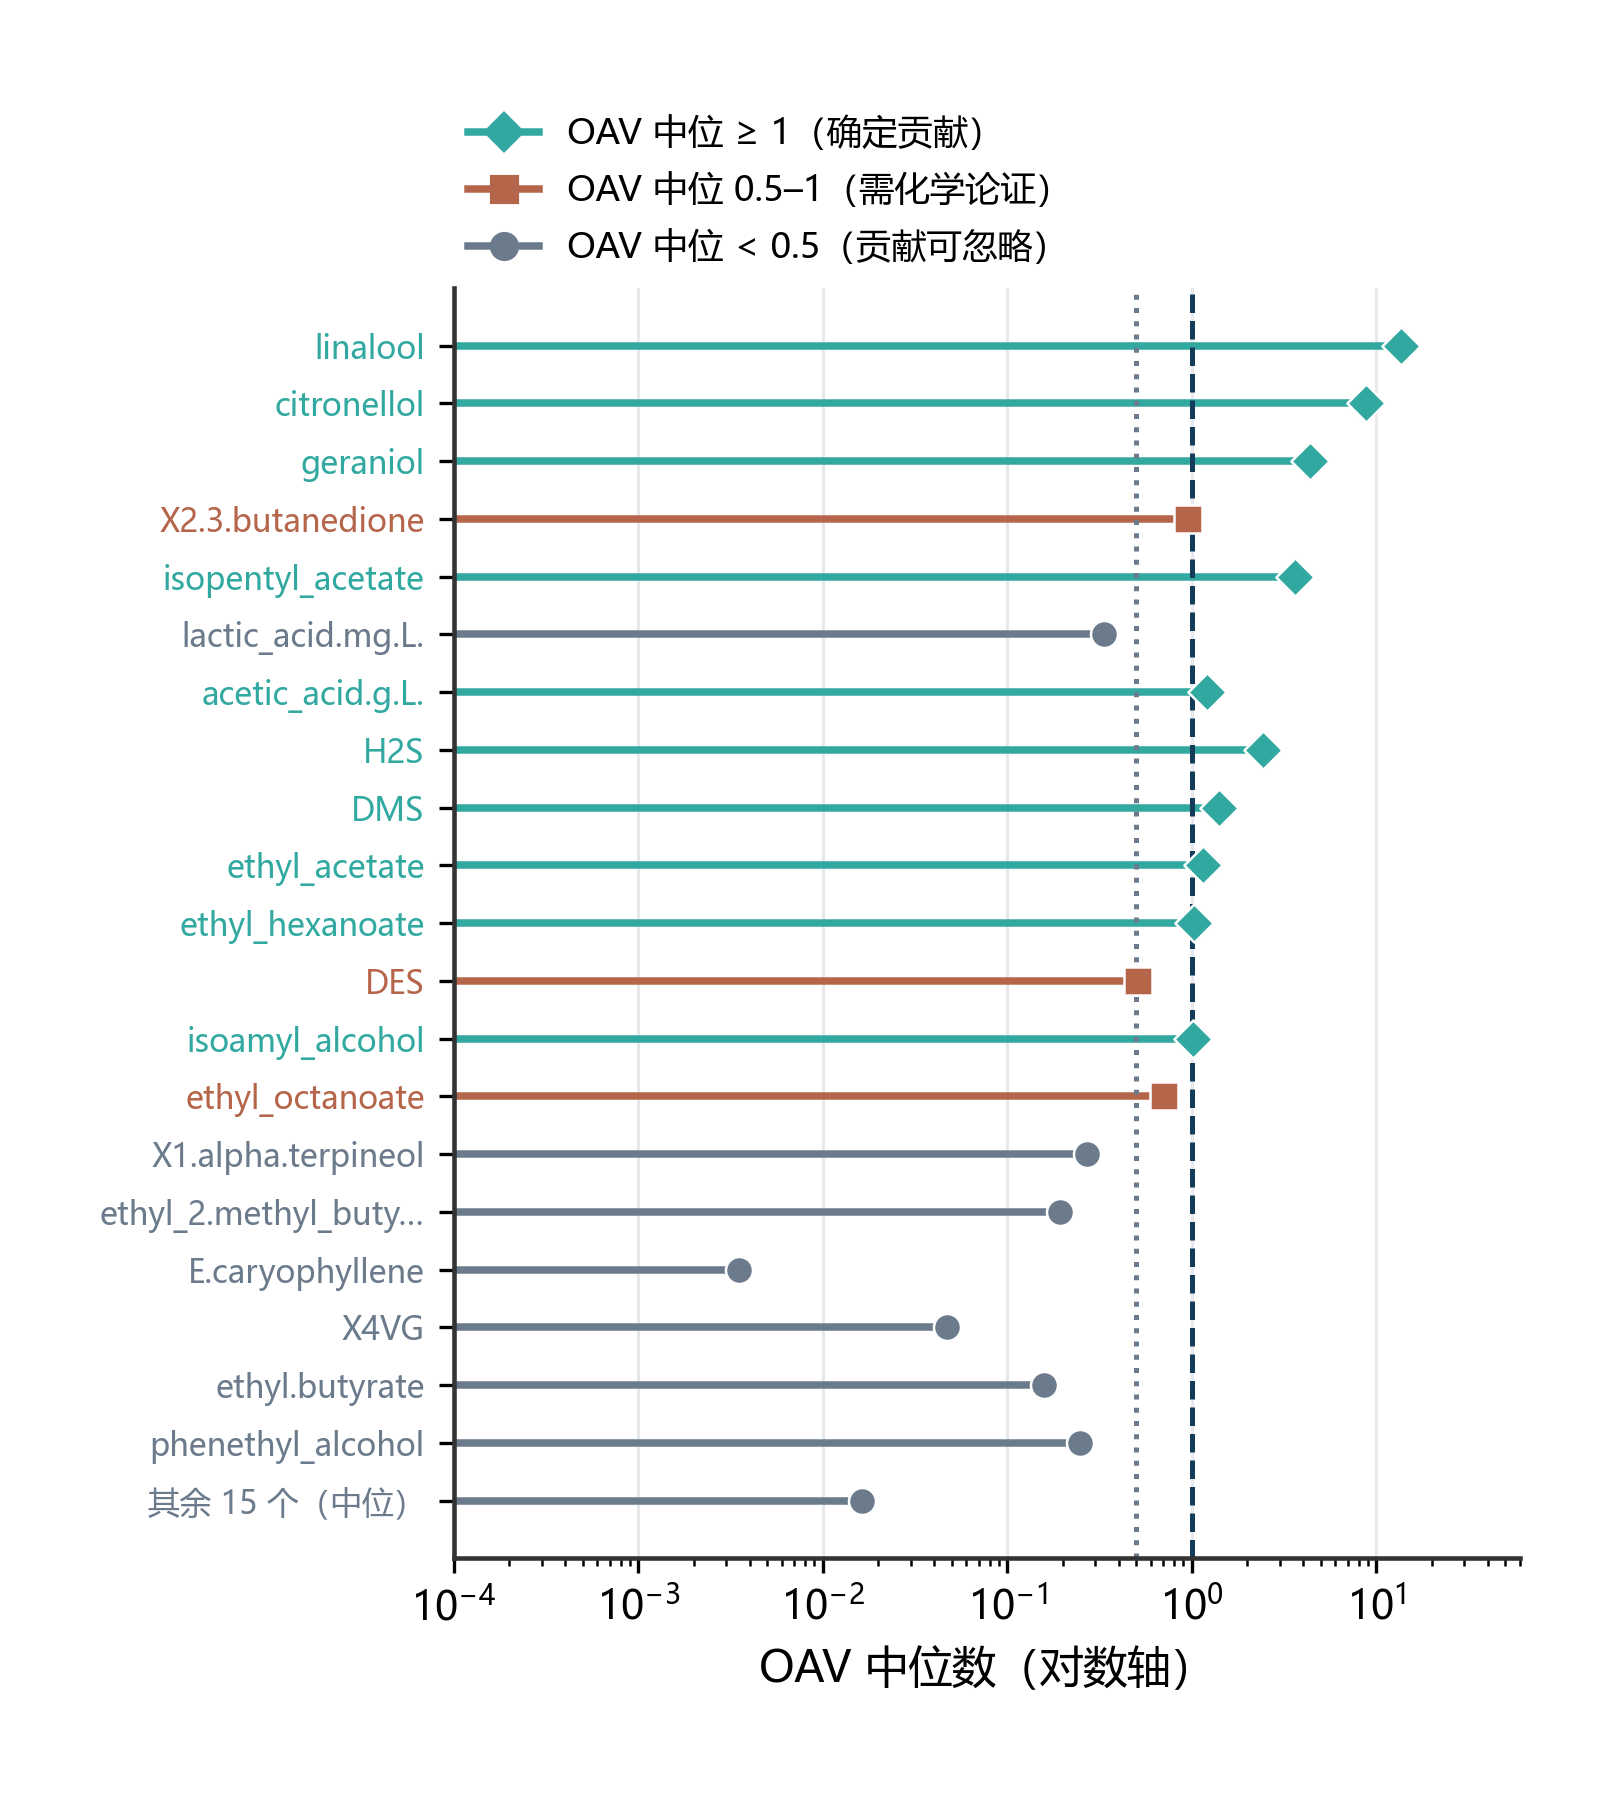
\includegraphics[width=\linewidth]{figures/fig_q2_oav.png}
\caption{化合物 OAV 排序与三档阈值线，纵轴取对数。高于 1 者具备被感知的物质基础}
\label{fig:q2oav}
\end{subfigure}
\hfill
\begin{subfigure}[t]{0.48\textwidth}
\centering
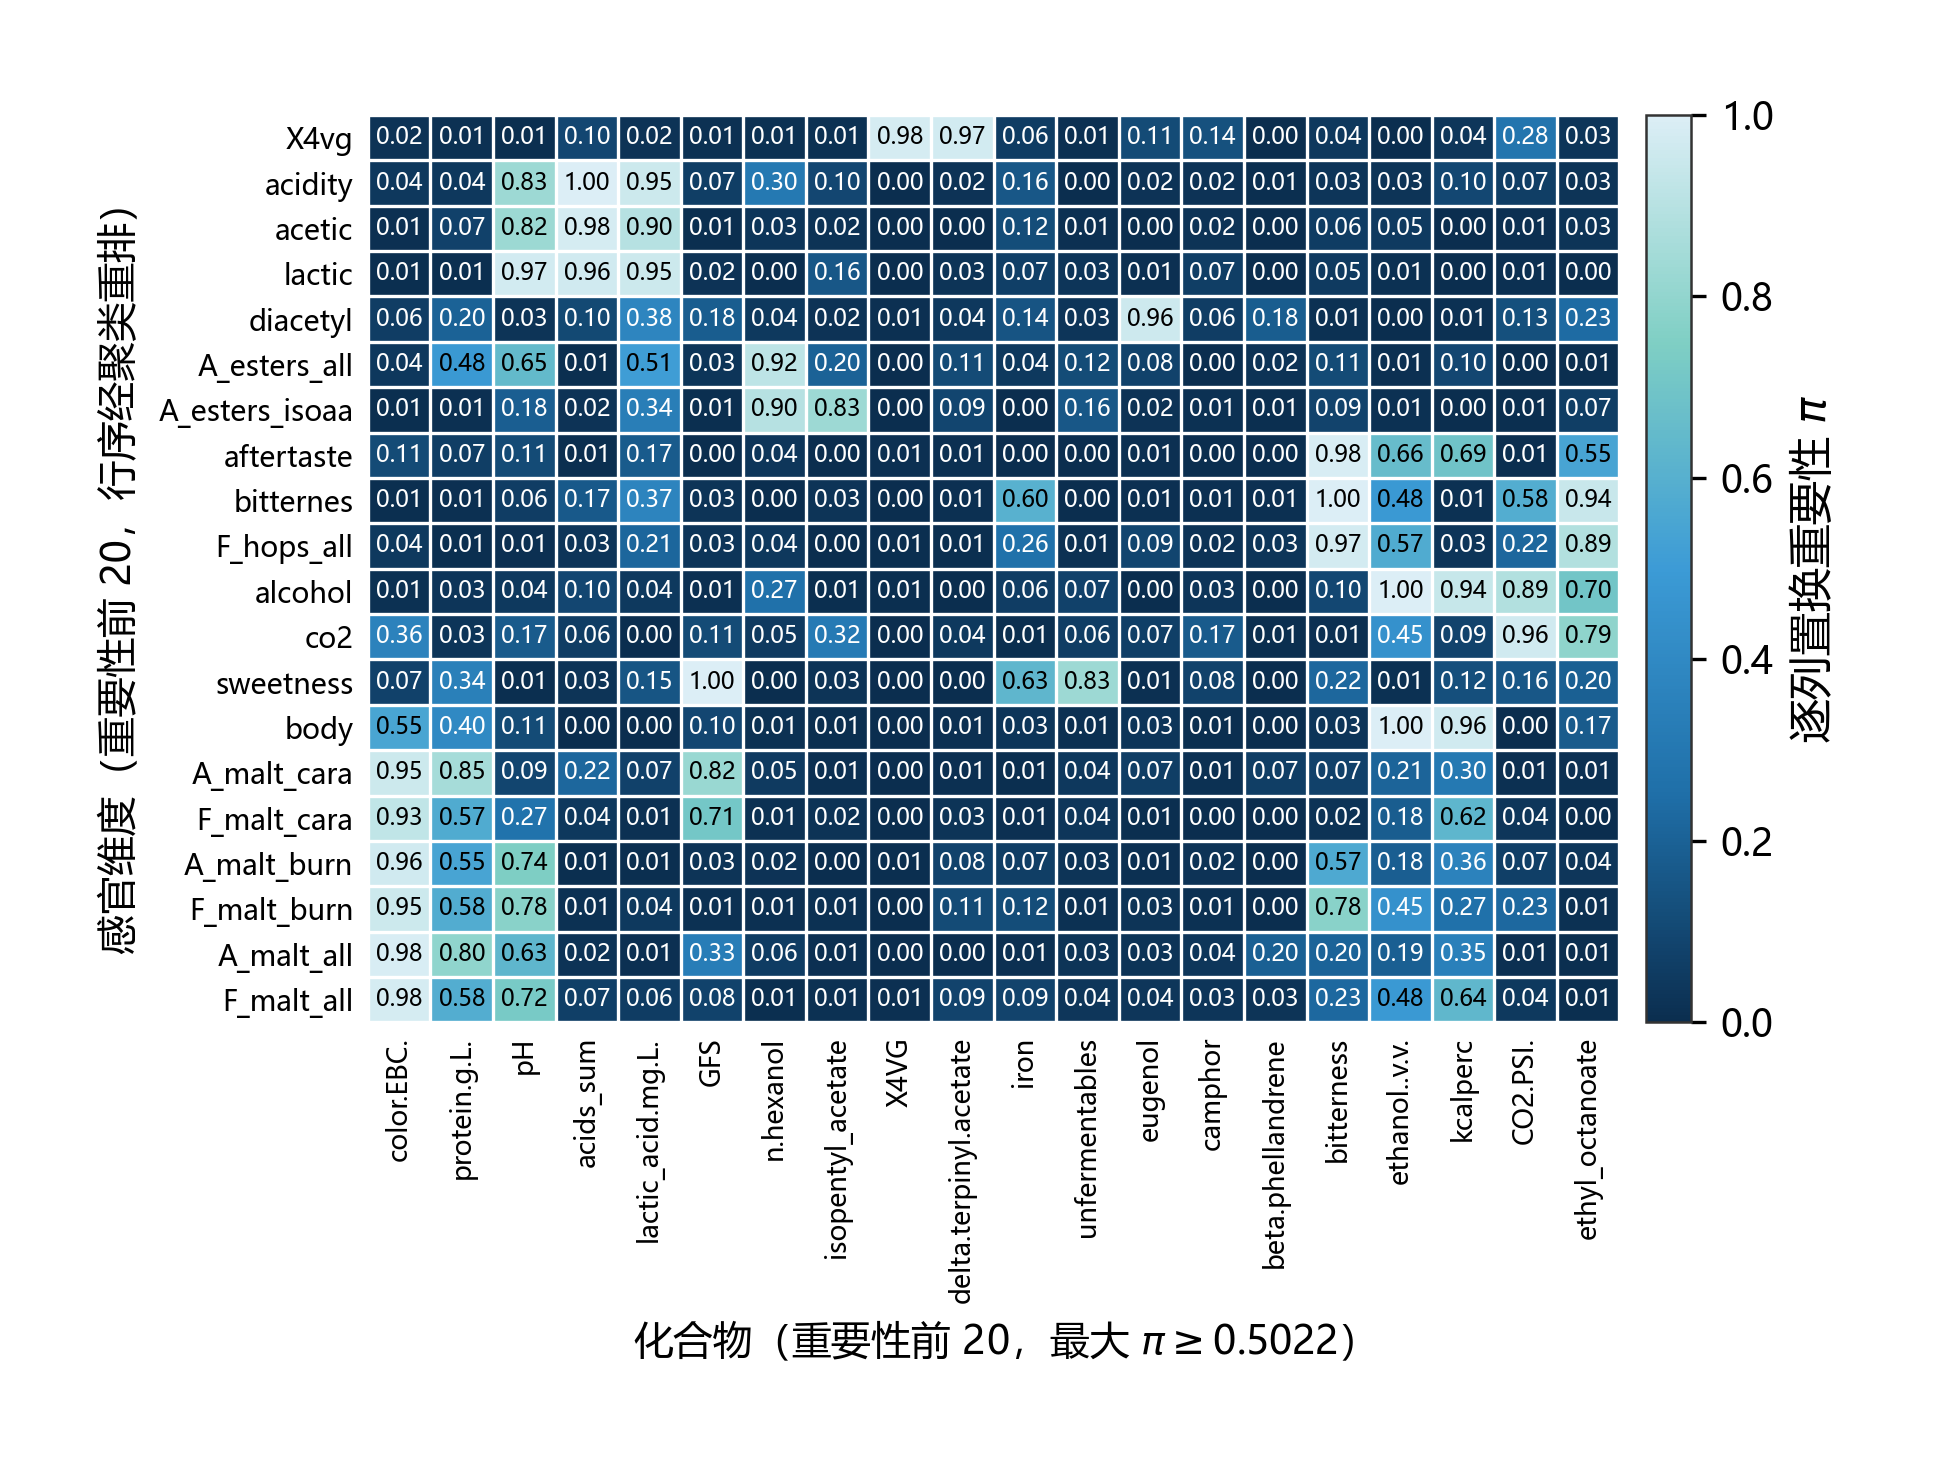
\includegraphics[width=\linewidth]{figures/fig_q2_pi_heatmap.png}
\caption{化合物与感官项的置换重要性矩阵：横轴为 50 个感官项，纵轴为化合物，颜色为 $\pi$ 的大小}
\label{fig:q2heat}
\end{subfigure}
\caption{化学合理性与归因全貌。左图为化合物 OAV 排序与三档阈值线（纵轴取对数），高于 1 者具备被感知的物质基础；右图为置换重要性矩阵}
\end{figure}

图~\ref{fig:q2heat} 给出化合物与感官的置换重要性矩阵：重要性集中于少数几列，其高值区与化学族一一对应。



稳定性是必须如实披露的短板。跨模型 Top-10 的 Jaccard 中位只有 0.0974，四分位距 0.0984，最小 0.0175、最大 0.2533(图~\ref{fig:q2jac})。这说明在 250 个样本、219 列强共线的条件下，Top-3 名单高度依赖模型族。因此本文的交付方式是：只把 A 档 19 条作为统计与化学两个条件的交集报告，C 档 40 条标注为“需额外化学论证”,N 档 83 条不进入结论，并在支撑材料里给出稳定性数值供复核。

逐项不稳定可以用比 Jaccard 更直接的方式量化。200 次重采样给出每个化合物在每个感官项上的平均排名 consrank，1 为最靠前，据此定义“稳定进前 $k$”的子集：以 $k=5$ 计，50 项中有 40 项连一个化合物都凑不出；即使只看每项第 1 名，consrank 中位也高达 11.8。在 250 个样本、219 列强共线的条件下，“每项各选三类关键化合物”本身就不是数据能稳定回答的问题。

因此本文补一条更稳的读法：不逐项选，而是问“哪些化合物在多个感官项上同时稳定靠前”。这个问法要求同一化合物在多个项上同时排名靠前，随机噪声很难同时抬高它在十几个独立拟合中的名次，因此稳定性自然提高。结果见表~\ref{tab:q2consensus}。

\begin{table}[htbp]
\centering
\small
\caption{跨感官项的共识归因，按进入前 5 名的项数降序，列出前 8 位}
\label{tab:q2consensus}
\begin{tabular*}{\textwidth}{@{\extracolsep{\fill}}lcc@{}}
\toprule
\textbf{化合物} & \textbf{前 5 名的项数} & \textbf{前 3 名的项数} \\
\midrule
\texttt{lactic\_acid}（酸感、酯香、酒体） & 13 & 9 \\
\texttt{acetaldehyde}（青苹果、溶剂） & 10 & 10 \\
\texttt{DMS}（熟蔬菜） & 9 & 1 \\
\texttt{phenethyl\_alcohol}（玫瑰花香） & 8 & 6 \\
\texttt{beta.phellandrene}（果香） & 8 & 5 \\
\texttt{prenyl.isobutyrate}（麦芽香） & 7 & 2 \\
\texttt{X1.10.di.epi.cubenol}（果香） & 7 & 6 \\
\texttt{X2.acetylfuran}（焦糖香） & 6 & 4 \\
\bottomrule
\end{tabular*}
\end{table}

这八位的化学解释都站得住：乳酸是酸感的直接物质基础，同时通过 pH 影响酯类的水解速率，因此在酸感、酯香、酒体三类上同时靠前；乙醛是发酵中间产物，带青苹果与溶剂气味，在麦芽香与后味上一致出现；DMS 是熟蔬菜味的缺陷物，但同时会干扰酒花香的判断，因此在前 5 名频繁出现而在前 3 名罕见——这一差异本身就说明它的作用是被“减去”而非“加上”；苯乙醇与辛酸乙酯分别是玫瑰花香与果香的主体，与酿造学一致。

两种读法回答不同的问题：逐项 Top-3 回答“某一感官项的化学来源”，只有 19 条通过双条件；跨项共识回答“整个风味体系的枢纽化合物”，即上表 8 位。前者细而不稳，后者粗而稳，本文并列报告而不偏取其一。

正结果的边界也须说明：统计显著性与预测能力不是同一件事。$R^2$ 最低的若干项如 barnyard 与 stale\_hops，在问题二同样只有很弱的重要性，两问方向一致；反之不成立。

%==============================================================================
% 八、问题三的模型建立与求解
%==============================================================================
\section{问题三：风味指纹的生成与重构}

\subsection{建模思路}

问题三要做三件事：以风格为条件生成合理的化合物谱、给出它的感官画像、再做跨风格迁移并保证缺陷物不恶化。

第一步的困难在样本量。22 个风格里最小的只有 3 款酒，即 Faro 风格，多数不超过 20 款。\emph{条件变分自编码器}、\emph{条件生成对抗网络}这类方法在此规模上无法估计条件分布\cite{xu2019}，本文列为不适用方法，不作主方案。实际采用更朴素的做法：在每个风格内部估计一个\emph{多元正态分布}，协方差用 \emph{Ledoit--Wolf 收缩法}\cite{ledoit2004}估计。样本少时直接用样本协方差会严重高估方差方向，收缩后向对角阵靠拢，生成样本不会离实测太远；收缩强度由数据算出，不手工设定。

第二步需要一个由化学谱计算感官的模型。本文用\emph{偏最小二乘回归}\cite{wold2001}，取 8 个成分，成分数由 5 折交叉验证确定。选它而不选树模型，是因为后续要解的是线性\emph{混合整数线性规划}，需要可线性化的结构，树模型写不进规划。

第三步的困难在于“不恶化”是硬要求，不能折成罚项。本文把它写成显式线性约束，与另外两个目标一起用\emph{$\varepsilon$-约束法}\cite{mavrotas2009}求解，并以\emph{NSGA-II}\cite{deb2002}作启发式对照，用支配关系与超体积判断精确解是否值得。

\subsection{决策变量与可行域}

若直接对 231 维做优化，模型里会混入大量化学上不可干预、或实际零改动的列。本文按“问题二 Top-3 的并集、香气类化合物、三个必然缺陷物”的规则把决策维降到 75 维
\begin{equation}
  \mathcal{J}=\Big(\bigcup_{s=1}^{50}\mathcal{T}_s\cap\text{香气类}\Big)\cup\{\text{DMS},\ \text{X4VG},\ \text{diacetyl}\},
  \qquad |\mathcal{J}|=75,
\end{equation}
这样既保留全部可干预的香气物质，又把优化规模压到可精确求解的量级。注意这一步是问题二向问题三的真实传递：没有 Top-3 并集，决策维无从收缩。

生成模型对目标风格 Tripel(28 个样本)估计多元正态，协方差取收缩估计
\begin{equation}
  \hat{\boldsymbol\Sigma}=(1-\delta)\boldsymbol{S}+\delta\,\mu\,\boldsymbol{I},
\end{equation}
其中 $\boldsymbol{S}$ 为样本协方差，$\delta=0.6844$ 由数据估出，$\mu$ 为平均方差。可行域由每一列在 250 款酒全体上的 1\% 与 99\% 分位界定。

生成像不像，用\emph{最近邻距离}检验：若生成样本与最近实测样本的距离远小于实测彼此的距离，说明它在复制；远大于则说明跑到了数据分布之外。实测生成样本的最近邻距离中位 13.6019，真实样本 12.6409，比值 1.076；只有 22.5\% 的生成样本比真实样本的中位距离更近。两项都接近理想值，生成器既没退化为复制，也没脱离分布。

表~\ref{tab:q3gen} 抽取三类化合物对照。三行缺陷物的生成中位分别为 1.52、$-1.82$、0.72，与 Tripel 实测中位 1.59、$-2.01$、0.29 相比方向并不一致：DMS 略降（1.52 vs 1.59），而 4VG 与双乙酰反而升高（$-1.82$ vs $-2.01$、0.72 vs 0.29）。这说明生成器描述的是“风格均值附近的合理扰动”，它不负责把缺陷物压到阈值以下——缺陷约束是在优化阶段才施加的，这也是表中 DMS 的生成中位 1.52 高于阈值 $\log_{10}17.25=1.24$、而在表~\ref{tab:q3} 的解上被压到 1.24 以内（P4 到 0.59）的原因。

\begin{table}[htbp]
\centering
\footnotesize
\caption{Tripel 风格 200 组生成化合物谱与实测对照，取 $\log_{10}$ 域，区间为 5\%--95\% 分位}
\label{tab:q3gen}
\begin{tabular*}{\textwidth}{@{\extracolsep{\fill}}p{2.8cm}p{2.9cm}cp{1.0cm}cp{1.0cm}c@{}}
\toprule
\textbf{化合物} & \textbf{字段名} & \textbf{类别} & \textbf{生成中位} & \textbf{生成区间} & \textbf{实测中位} & \textbf{实测区间} \\
\midrule
二甲基硫（熟蔬菜味） & DMS & 缺陷 & 1.52 & [0.59, 2.17] & 1.59 & [1.22, 2.02] \\
4-乙烯基愈创木酚（辛香） & X4VG & 缺陷 & -1.82 & [-2.01, -0.37] & -2.01 & [-2.01, -0.92] \\
双乙酰（奶油味） & X2.\allowbreak 3.\allowbreak butanedione & 缺陷 & 0.72 & [0.00, 3.51] & 0.29 & [0.00, 1.50] \\
乙醛（青草味） & acetaldehyde & 香气 & 0.91 & [-0.75, 1.20] & 0.81 & [0.53, 1.03] \\
异戊酸乙酯（果香） & ethyl\_\allowbreak isovalerate & 香气 & -2.88 & [-4.49, -1.02] & -2.39 & [-4.49, -1.80] \\
异丁酸异戊烯酯（果香） & prenyl.\allowbreak isobutyrate & 香气 & 5.29 & [2.46, 7.09] & 5.17 & [4.49, 5.94] \\
松油烯-4-醇（木香） & terpinen.\allowbreak 4.\allowbreak ol & 香气 & 5.10 & [2.92, 7.31] & 5.22 & [4.19, 6.66] \\
苯乙醛（蜂蜜香） & phenylacetaldehyde & 香气 & 0.12 & [0.00, 0.24] & 0.02 & [0.00, 0.08] \\
\bottomrule
\end{tabular*}
\end{table}

\subsection{感官代理模型}

优化需要把感官预测写进约束。偏最小二乘回归先把 231 维化学谱投影到低维潜变量，再回归到 50 维感官，得到线性映射
\begin{equation}
  \hat y_s(x)=a_s+\sum_{j\in\mathcal{J}}b_{sj}x_j,\qquad s=1,\dots,50,
\end{equation}
系数 $b_{sj}$ 直接构成约束矩阵。成分数用 5 折交叉验证在 $\{2,3,4,6,8,10,13,16,20\}$ 里选，落在 8。

代理的精度决定了前沿的可信度。逐项交叉验证 $R^2$ 中位 0.1386(47/50 为正)，绝对误差中位 0.4626、95 分位 1.4124、最大 3.1525，且 50 项的最大误差全部超过各自一个标准差。图~\ref{fig:q3cvr2} 与图~\ref{fig:q3err} 分别给出逐项拟合能力与误差量级。

\begin{figure}[htbp]
\centering
\begin{subfigure}[t]{0.48\textwidth}
\centering
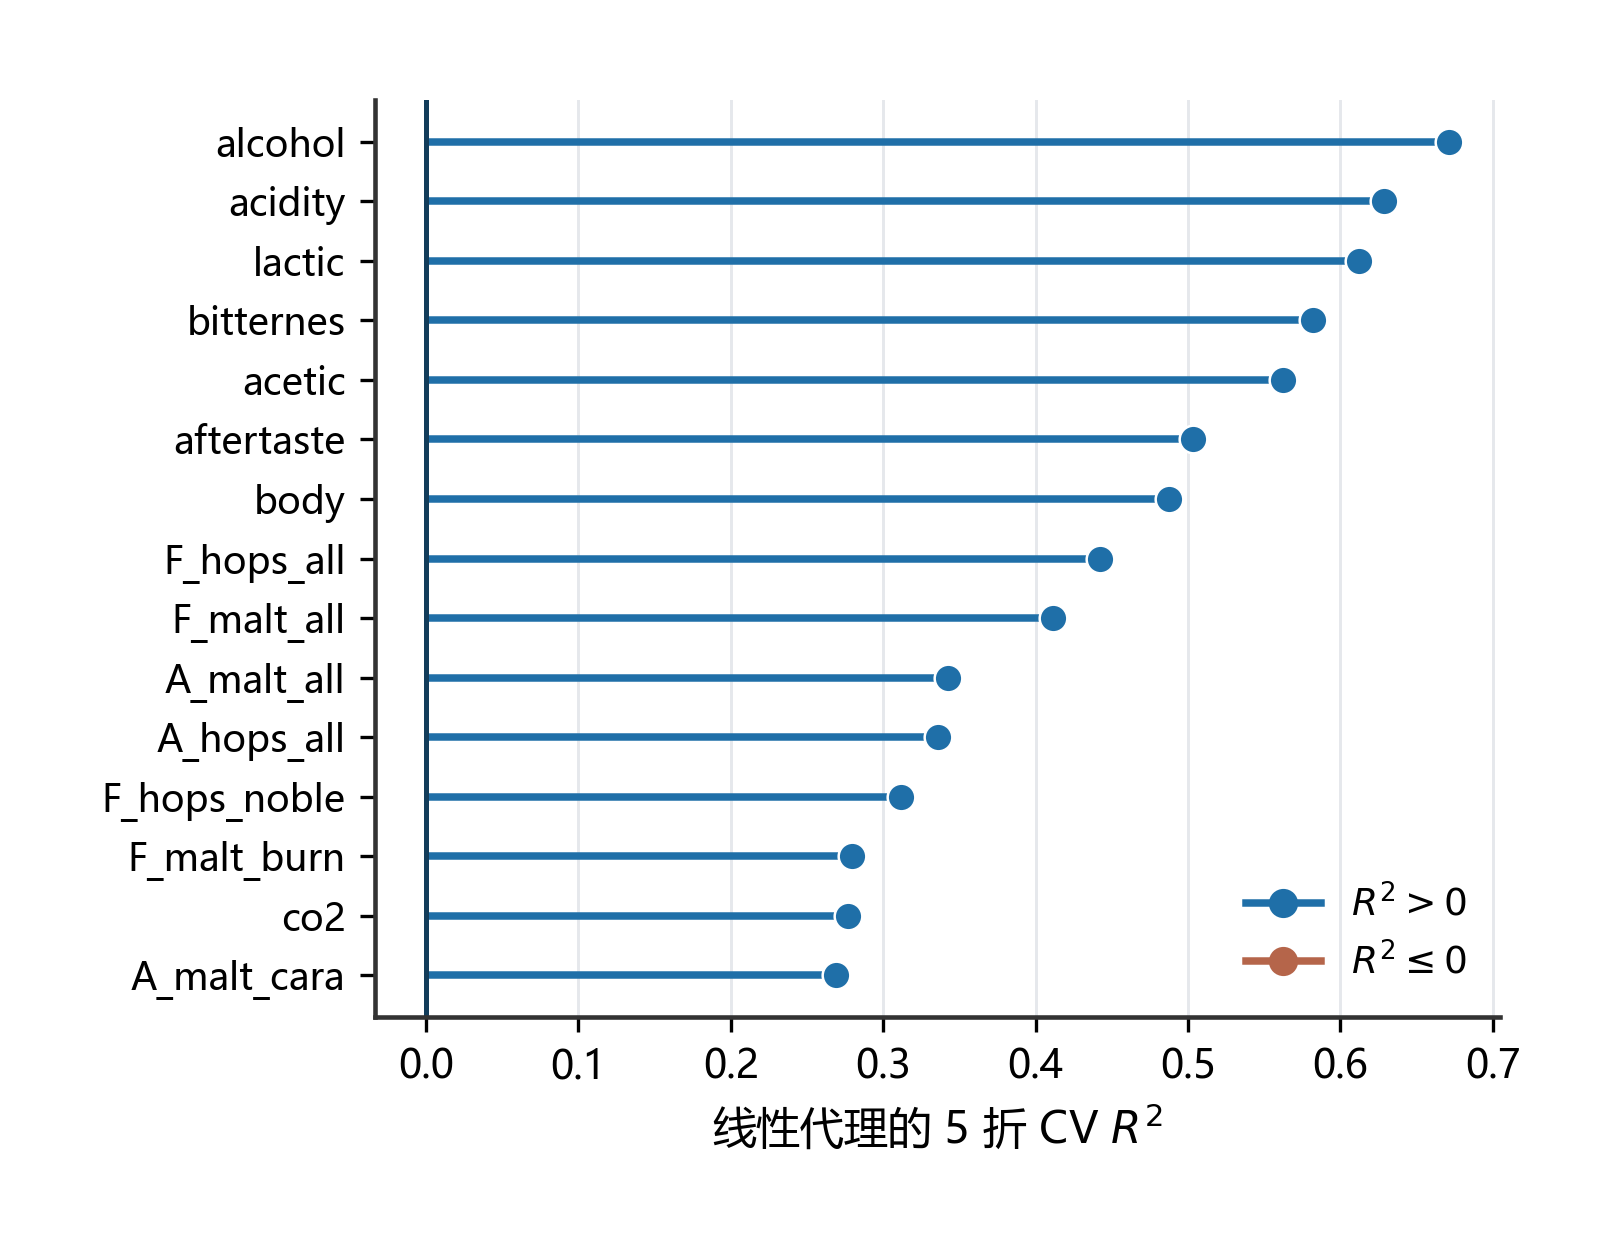
\includegraphics[width=\linewidth]{figures/fig_q3_surrogate_cv.png}
\caption{逐项交叉验证 $R^2$}
\label{fig:q3cvr2}
\end{subfigure}
\hfill
\begin{subfigure}[t]{0.48\textwidth}
\centering
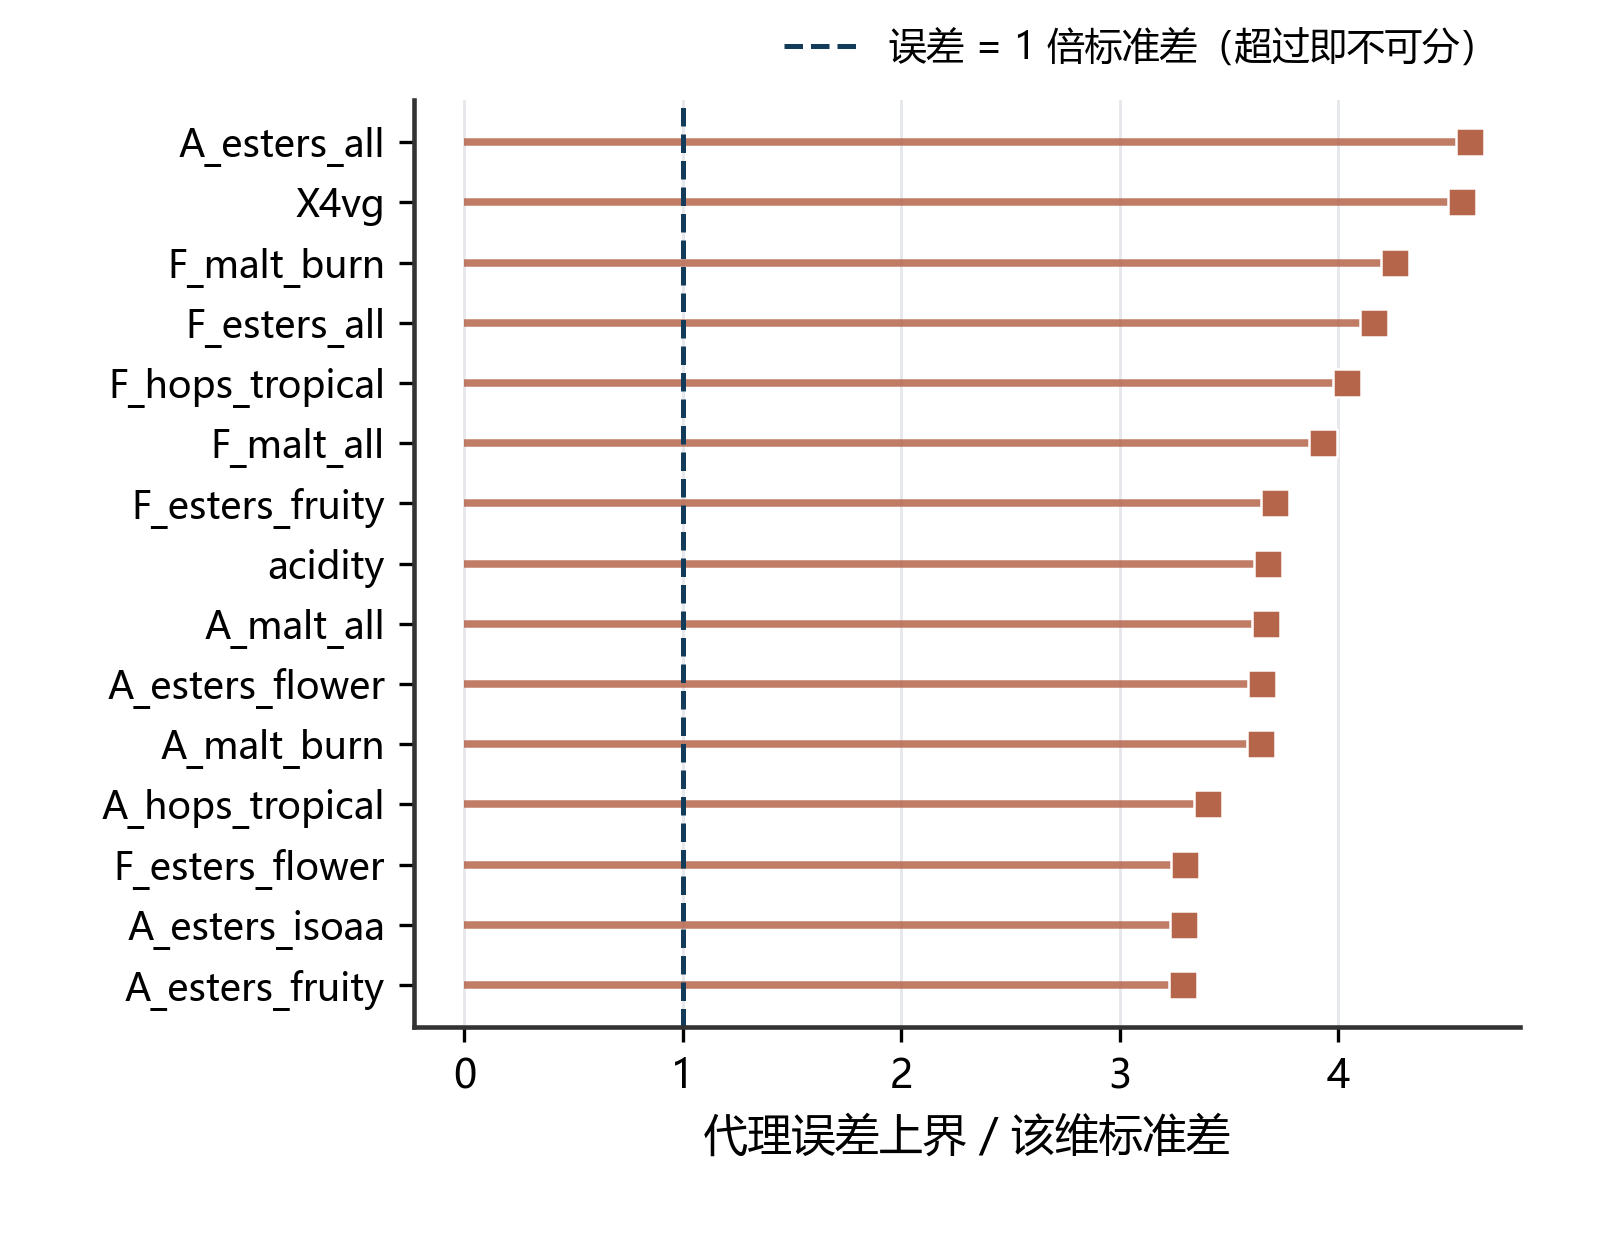
\includegraphics[width=\linewidth]{figures/fig_q3_surrogate_err.png}
\caption{误差与标准差之比}
\label{fig:q3err}
\end{subfigure}
\caption{感官代理的精度。左图为逐项 $R^2$，中位 0.1386；右图为误差与标准差之比，50 项的最大误差全部超过 1 倍标准差}
\end{figure}

两图合起来说明一件事：代理足以支撑“往哪个方向调”的判断，但不足以支撑“哪个点更好”的判断。这一结论在 8.4 节解释前沿可信边界时会直接用到。

\subsection{多目标混合整数线性规划}

以 $\log_{10}$ 域的浓度 $x_j$ 为决策变量，原始样本的浓度记为 $x_j^0$。三个目标定义为
\begin{align}
  f_1(x)&=\sum_{s=1}^{50}\frac{1}{\hat\sigma_s}\left|\hat y_s(x)-t_s\right|, \\
  f_2(x)&=\sum_{k\in\mathcal{K}}\max\left\{0,\ \frac{d_k(x)}{\tau_k}-1\right\}, \\
  f_3(x)&=\sum_{j\in\mathcal{J}}\left|x_j-x_j^0\right|,
\end{align}
$f_1$ 为按感官标准差加权的 $L_1$ 偏差，其中 $t_s$ 取目标风格内的中位感官值；$f_2$ 为缺陷物超阈值程度之和，$f_3$ 为干预代价。

约束分三类。硬约束要求 DMS 与 X4VG 不超阈值；软约束把双乙酰计入 $f_2$ 而不作硬限，因为其阈值在样本中位附近，硬压会与实际工艺相悖
\begin{equation}
  d_k(x)\le\tau_k,\quad k\in\{\text{DMS},\text{X4VG}\};\qquad
  d_{\text{diacetyl}}(x)\ \text{入}\ f_2 .
\end{equation}
改动量约束限制同时改动的化合物个数，以保证“定向重构”的工艺含义
\begin{equation}
  \sum_{j\in\mathcal{J}}z_j\le k_{\max}=25,\qquad
  \left|x_j-x_j^0\right|\le M_j z_j,\qquad z_j\in\{0,1\}.
\end{equation}
绝对值项经 $u_j\ge x_j-x_j^0$、$u_j\ge x_j^0-x_j$ 线性化，$f_1$ 中的 $|\hat y_s(x)-t_s|$ 同样拆成正负偏差变量。由此得到带 75 个 0--1 变量、326 个变量、406 条约束的混合整数线性规划，用 \emph{Gurobi 13.0.2} 求解。

三目标不可加权求和，因为 $f_1$、$f_2$、$f_3$ 的物理含义完全不同。本文用 $\varepsilon$-约束法：先分别解三个单目标得到支付表，再在 $f_2$、$f_3$ 的取值区间内取 $20\times15=300$ 个网格点，逐点求
\begin{equation}
  \min\ f_1(x)\quad \text{s.t.}\quad f_2(x)\le\varepsilon_2,\ f_3(x)\le\varepsilon_3,
\end{equation}
并加增广项剔除弱 Pareto 点。300 个网格点中 280 个可行，且这 280 点全部非支配，说明前沿的形状完全由目标之间的权衡决定，不是被可行性边界截断。

作为对照，本文手写 \emph{NSGA-II}：SBX 交叉 $\eta=15$、多项式变异 $\eta=20$，种群与代数按 75 维设定，在同样的缺陷物约束下得 115 个非支配点。

\subsection{模型求解}

\noindent\textbf{三个目标的无量纲化}\quad 三个目标的量级差别很大，直接加权会让感官偏差独占主导。因此先求理想点与最差点：单独最小化 $f_1$ 时得 $f_1=13.5064$、$f_2=87.1989$、$f_3=26.7886$；单独最小化 $f_2$ 时得 $f_1=48.7011$、$f_2=0$、$f_3=9.1529$；单独最小化 $f_3$ 时得 $f_1=47.2083$、$f_2=87.1989$、$f_3=1.0222$。由此得 $f_2$ 的极差为 87.1989、$f_3$ 的极差为 $26.7886-1.0222=25.7664$，归一化时按各自极差缩放。求理想点的 3 次求解中共有 20 个网格点不可行，为保持比较基准一致，理想点取在可行集内。

\noindent\textbf{ε-约束与网格}\quad 多目标按 ε-约束法处理：每次把 $f_2$、$f_3$ 各固定在一个水平上写成约束，只优化 $f_1$，遍历 $(f_2,f_3)$ 的 $20\times15=300$ 个组合。300 次求解中 280 次可行、20 次因硬约束冲突不可行，280 个可行点全部非支配，筛选后保留 5 个 Pareto 点。硬约束逐物取“阈值”与“基线”中更严的一条，即上限 $=\min(\log_{10}T_k,\,x_k^{0})$：DMS 的阈值换算值 1.2368 低于基线，故上限取 1.2368；4VG 的文献阈值 0.206\,mg/L 换算到对数域约 $-0.686$，但基线 $-2.0132$ 已低于该阈值，故取更严格的基线上限 $-2.0132$，该值不是阈值的对数换算值，软约束是双乙酰浓度不高于 0.2993，违约时以罚项 $\gamma=1.0$、权重 $\lambda=0.1$ 计入 $f_1$。

\noindent\textbf{求解规模与耗时}\quad 每个网格点对应一个混合整数线性规划：326 个变量（其中 75 个 0--1、251 个连续）、406 条约束，其中感官代理的 50 条线性等式由 8 成分偏最小二乘回归给出。求解器用 Gurobi，采用默认的自动算法选择，对偶单纯形与内点法按规模自动切换，300 个网格点串行求解总耗时 47.7 秒，单点平均 0.159 秒。这个速度使得 280 个点的全网格遍历比启发式搜索更划算，也解释了为什么本文没有采用 NSGA-II 作为主方案。

\noindent\textbf{结果的核验}\quad 生成是否退化为复制，用最近邻距离检验：生成谱到真实样本的最近邻距离中位 13.6019，真实样本彼此的最近邻距离中位 12.6409，比值 1.076，说明生成谱既未落进训练集的凸包内部，也没有外推到远离数据的高风险区域。前沿是否真的更优，用 NSGA-II 在相同约束下独立跑出的 115 个非支配点作对照：本文的 5 个精确点支配其中 105 个（91.30\%），反向支配为 0，超体积 688.54 对 299.12。

\subsection{结果分析}

5 个 Pareto 点全部为 OPTIMAL 状态，$mip\_gap=0$，两两互不支配，见表~\ref{tab:q3}。硬约束的超出量取 $t_k-\tau_k$，负值即低于阈值，在五点上的最小值为 $-0.644$(P4)，即最贴近阈值的那条约束仍留有余量。基线感官偏差为 48.9620，最优解 23.8519，降幅 51.3\%。

\begin{table}[htbp]
\centering
\footnotesize
\caption{问题三的 Pareto 前沿，以 Tripel 为目标风格}
\label{tab:q3}
\begin{minipage}{\textwidth}\footnotesize
注：五个点的 $f_2$ 均为 0.0000，缺陷维度在本例中不活跃，前沿实际是 $f_1$--$f_3$ 的二维权衡，$f_2$ 只作可行性校验。
\end{minipage}
\begin{tabular*}{\textwidth}{@{\extracolsep{\fill}}ccccc@{}}
\toprule
\textbf{点} & $f_1$（感官偏差） & $f_2$（缺陷风险） & $f_3$（改动代价） & \textbf{改动化合物数} \\
\midrule
P1 & 23.8519 & 0.0000 & 7.4510 & 7 \\
P2 & 25.2188 & 0.0000 & 6.4250 & 6 \\
P3 & 27.1161 & 0.0000 & 5.3507 & 5 \\
P4 & 30.3666 & 0.0000 & 4.2891 & 4 \\
P5 & 37.3603 & 0.0000 & 2.1439 & 2 \\
\bottomrule
\end{tabular*}
\end{table}

这里要记录一处必要的单位处理。缺陷物阈值必须换算到各列在附件1 中的实际量纲域：DMS 与 4VG 在 $\log_{10}$ 域，双乙酰与 trans-2-壬烯醛在 mg/L 线性域(依据 5.3 节的逐列标记，并经附件8 的 Calibrated 表交叉验证)。若一律取 $\log_{10}$，线性域列的软约束会退化为与决策无关的常数，$f_2$ 被固定而失去意义。修正后 $f_2$ 能真正降到 0，这一变化本身就是“约束是否在起作用”的检验。

五个点的改动数单调递减：P1 改动乙醛、DMS、异戊酸乙酯、苯乙醛、异丁酸异戊烯酯、松油烯-4-醇与苯乙酸乙酯共 7 个；P2 去掉苯乙酸乙酯；P3 再去掉异戊酸乙酯，剩 5 个；P4 去掉松油烯-4-醇，剩 4 个；P5 换了一套组合，只改 DMS 与甲基吡嗪 2 个。前四点的改动集合逐级包含，说明前沿是从同一组化合物里逐步削减而成；第五点换了另一条路线，用最小干预换取可接受的偏差。真正被调动的化合物始终不出这 8 个，其余 67 个决策变量被阈值与改动上限卡住——这是一条可解释的结论：在给定阈值下能有效调节风味指纹的化合物是少数。

从改动方向看，见图~\ref{fig:q3opt}；DMS 在所有点上都被下调，从 1.587 压到 0.593 至 1.237 之间，取 $\log_{10}$ 域，阈值为 1.237；松油烯-4-醇从 5.222 直接降到检出限 $-1.818$，异戊酸乙酯从 $-2.390$ 降到 $-4.487$，乙醛从 0.808 降到 $-0.464$ 至 $-0.745$，异丁酸异戊烯酯从 5.169 降到 0.823。唯一上调的是苯乙醛，从 0.021 升到 0.238。DMS 是熟蔬菜味缺陷物，下调符合目标风格；松油烯-4-醇带木香与松节油气息，在 Tripel 的高酯香型中属可牺牲项；苯乙醛上调与 Tripel 的蜂蜜甜香一致。方向在酿造学上自洽，说明约束与代理没有把结果推向化学上荒谬的解。

\begin{figure}[htbp]
\centering
\begin{subfigure}[t]{0.48\textwidth}
\centering
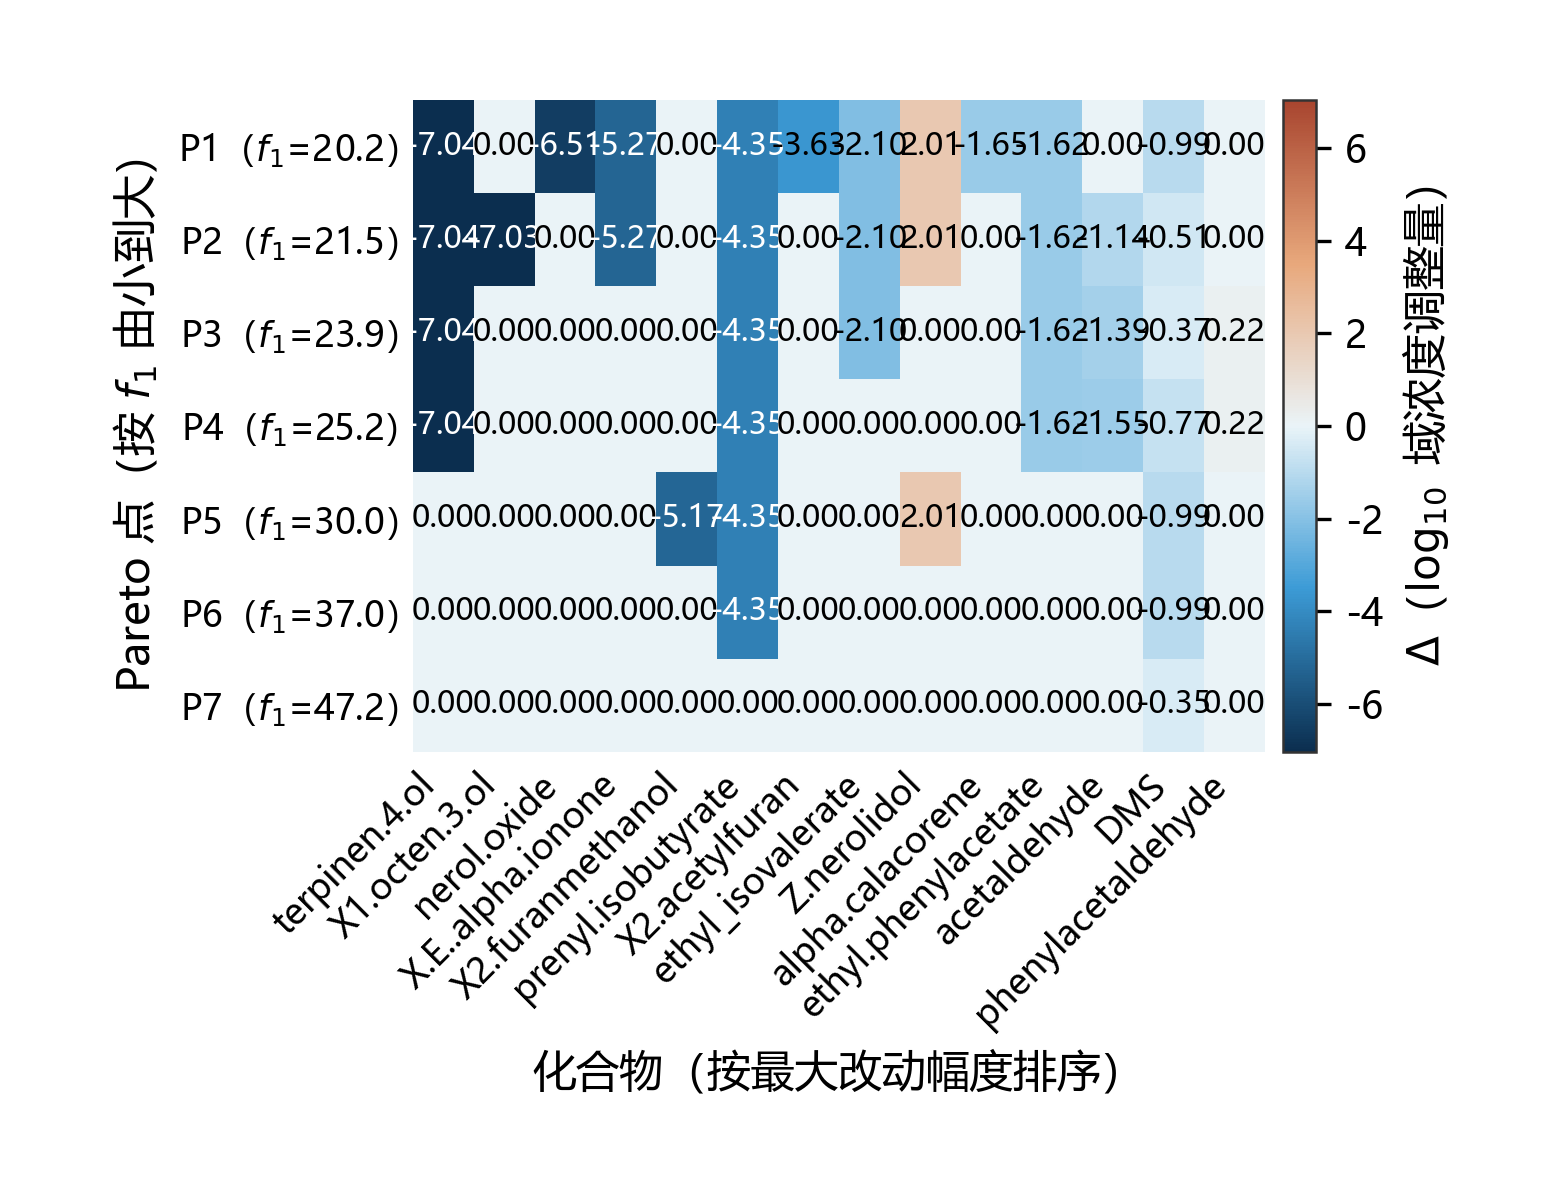
\includegraphics[width=\linewidth]{figures/fig_q3_deltas.png}
\caption{改动化合物与幅度}
\end{subfigure}
\hfill
\begin{subfigure}[t]{0.48\textwidth}
\centering
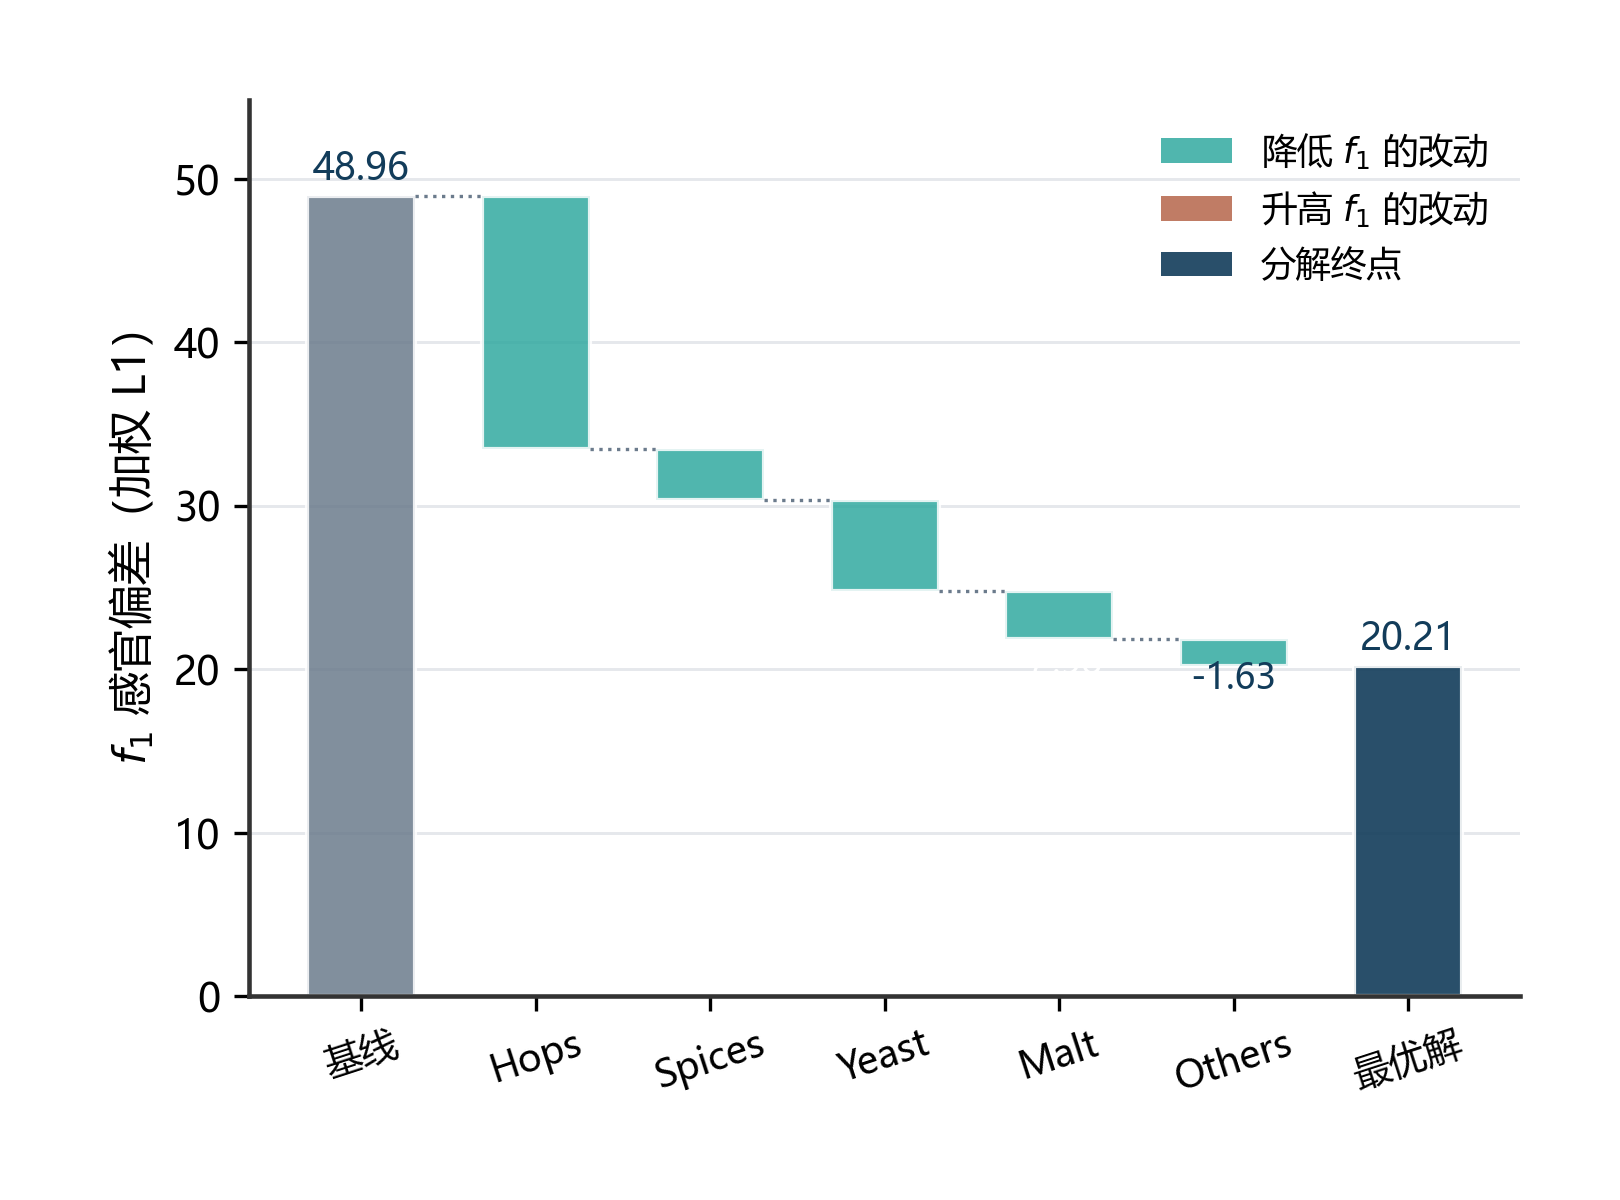
\includegraphics[width=\linewidth]{figures/fig_q3_waterfall.png}
\caption{$f_1$ 的逐组分解}
\end{subfigure}
\caption{最优解改了什么。左图为 8 个化合物的调整幅度，DMS 与松油烯-4-醇下调最重；右图为 $f_1$ 的逐组分解，降幅主要来自酸度、苦度与硫味三类}
\label{fig:q3opt}
\end{figure}

精确解与启发式的对比是本章的第二个结论。5 个精确点支配了 115 个 NSGA-II 点中的 91.30\%，反向支配比例为 0；超体积 688.54 对 299.12，增益 389.42(图~\ref{fig:q3front})。这为“以精确混合整数规划为主、启发式为对照”的路线提供了机械证据。

\begin{figure}[htbp]
\centering
\begin{subfigure}[t]{0.48\textwidth}
\centering
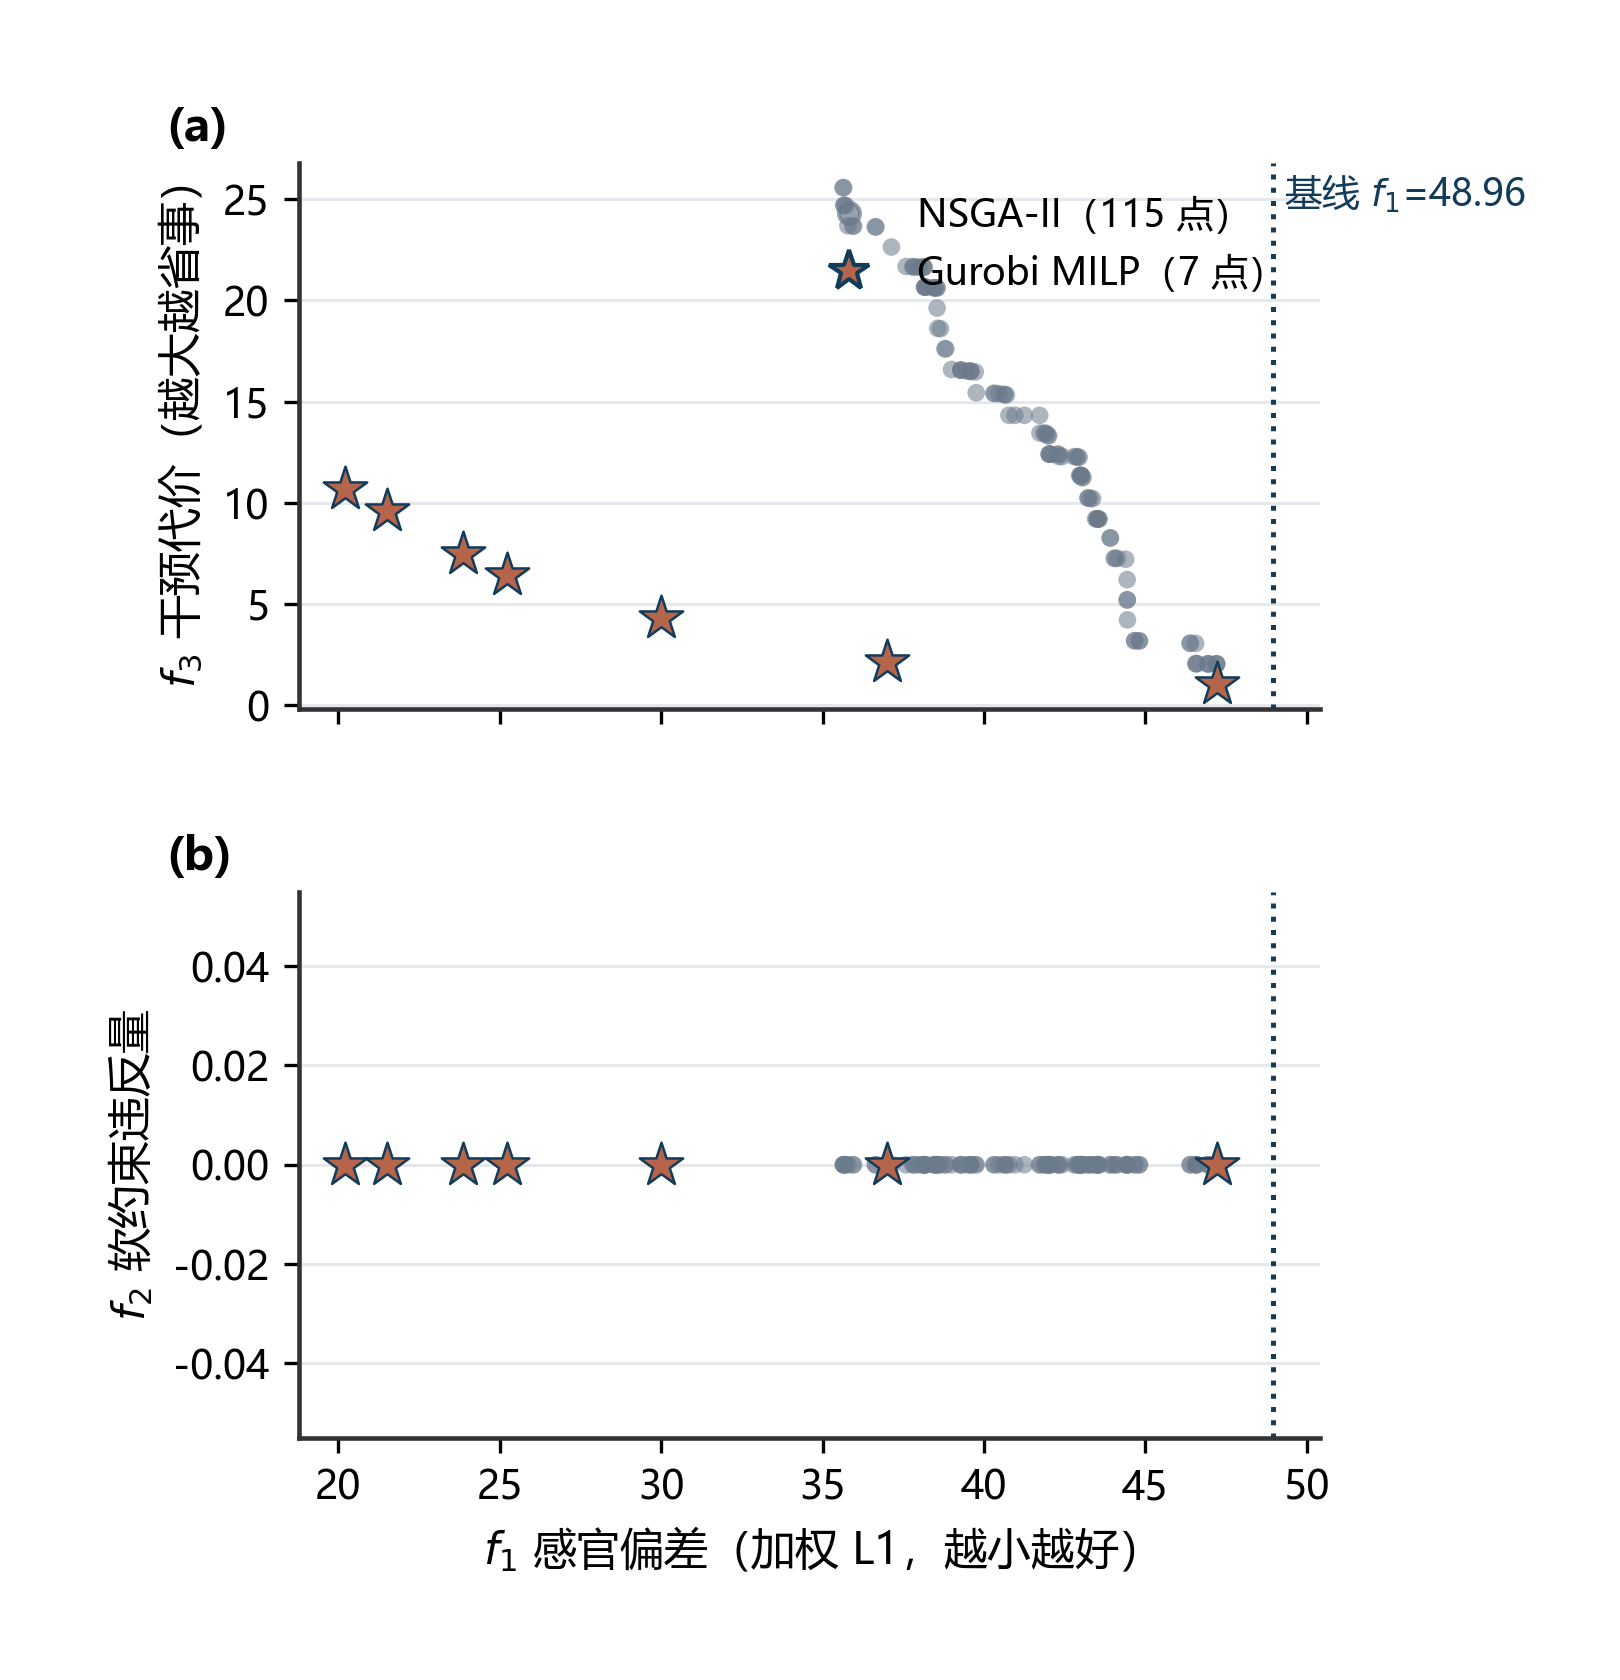
\includegraphics[width=\linewidth]{figures/fig_q3_front.png}
\caption{混合整数规划前沿与 NSGA-II 前沿的双投影对比：精确前沿整体位于启发式前沿的左下方}
\label{fig:q3front}
\end{subfigure}
\hfill
\begin{subfigure}[t]{0.48\textwidth}
\centering
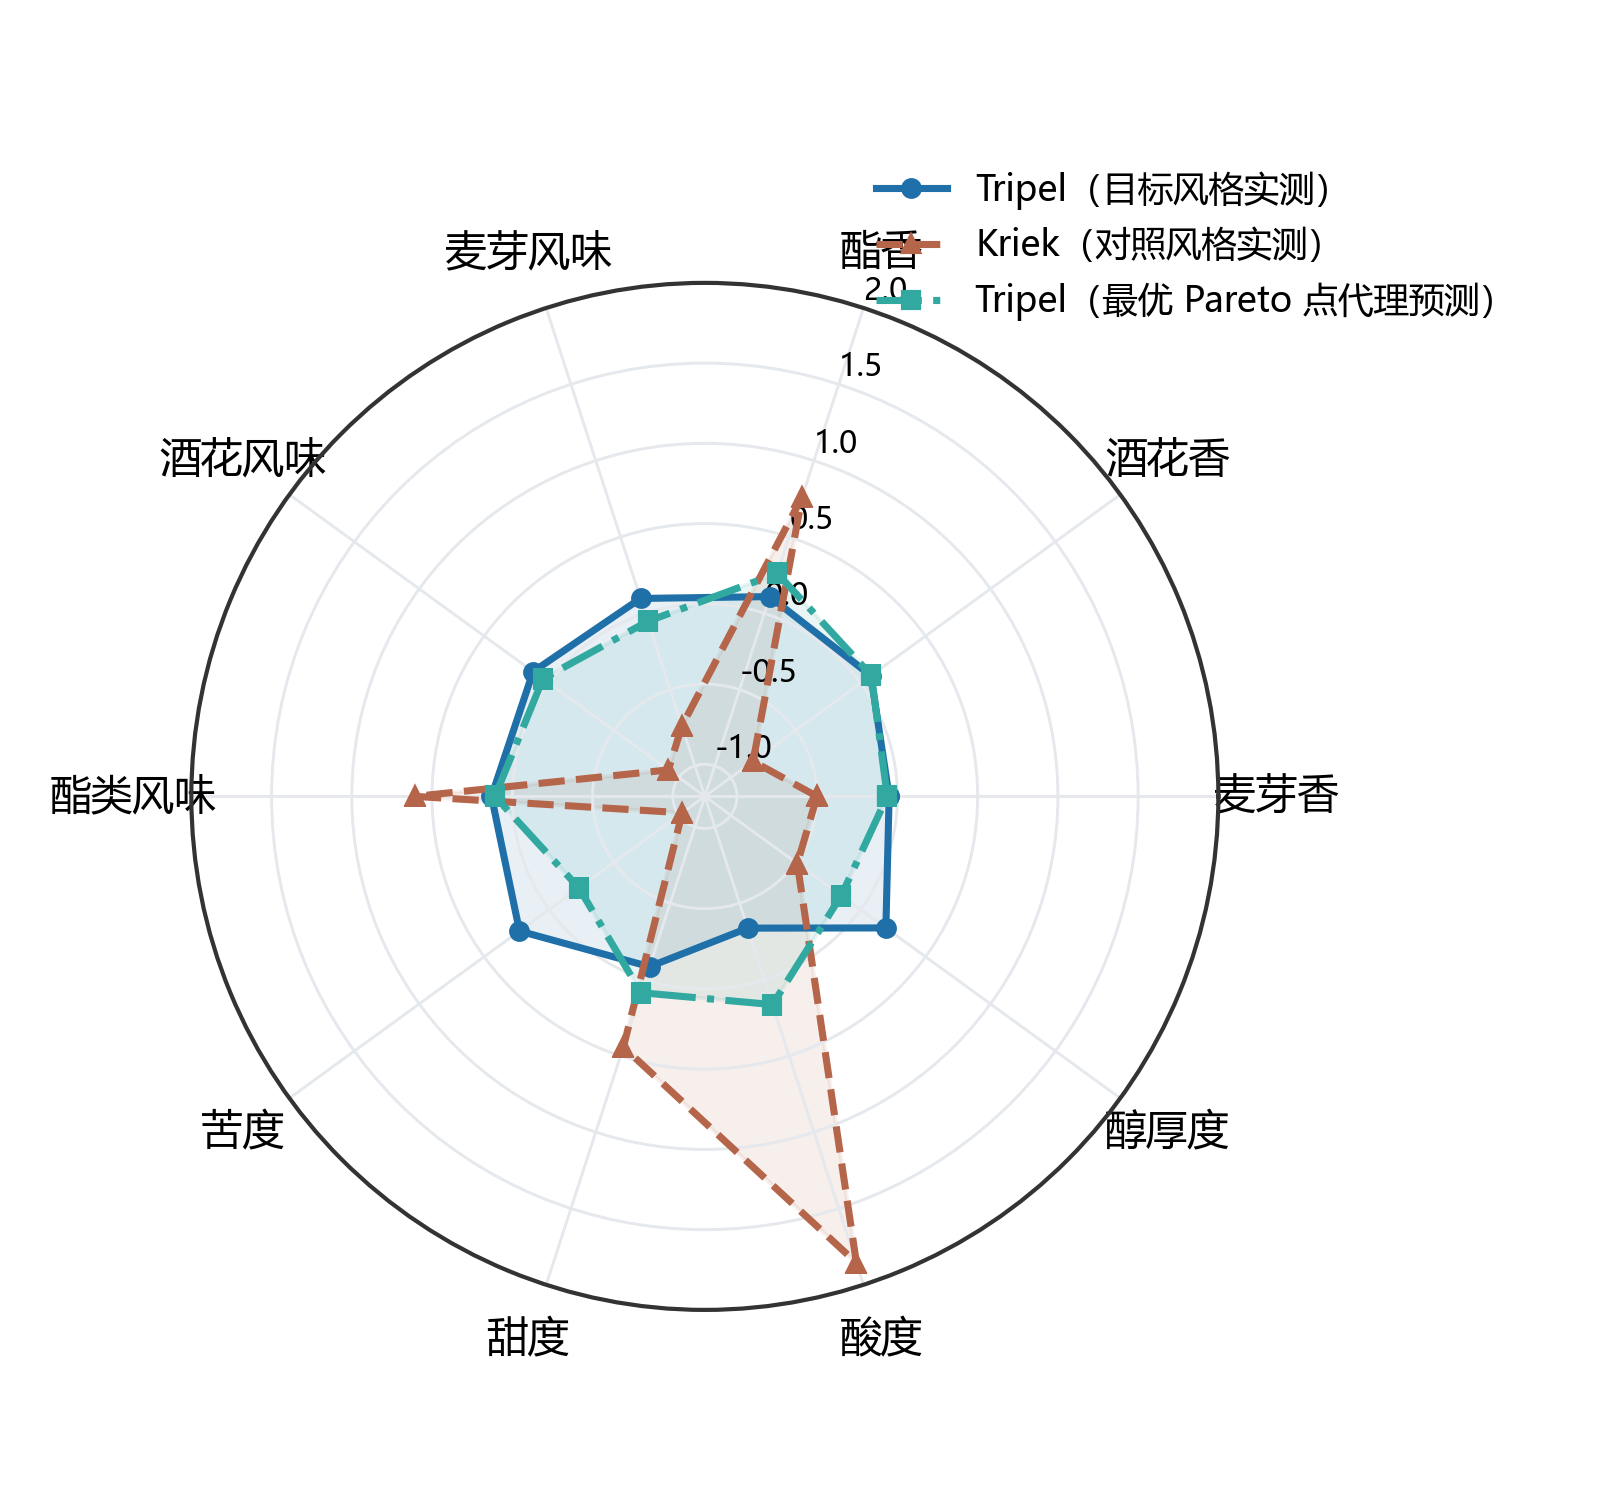
\includegraphics[width=\linewidth]{figures/fig_q3_radar.png}
\caption{目标风格、对照风格与最优解的感官画像：最优解在气味维度贴近 Tripel，在口感维度偏向 Kriek}
\label{fig:q3radar}
\end{subfigure}
\caption{前沿与画像。左图为混合整数规划前沿与 NSGA-II 前沿的双投影对比，精确前沿整体位于启发式前沿的左下方；右图为目标风格、对照风格与最优解的感官画像}
\end{figure}

第三个结论关系结果的可信边界。五点之间的 $f_1$ 间隙依次为 1.3669、1.8973、3.2505、6.9936，而代理误差中位 0.4626、95\% 分位 1.4124、上界 3.1525。P1 与 P2 的间距小于 95\% 分位误差，统计上不可分；P2 与 P3 略大于分位误差但仍小于上界，只能算弱可分；后两个间隙大于上界，可以分辨。因此本文把前沿报成三段(P1--P2、P3、P4--P5)，段内不作排序，也不指定唯一最优解。

图~\ref{fig:q3radar} 与表~\ref{tab:q3profile} 给出感官画像。气味描述类基本贴合目标：酒花香的嗅觉维度由 0.079 到 0.061、酯香的嗅觉维度由 0.109 到 0.180、苦度由 0.228 到 $-0.292$；口感类偏离较多：麦芽香的嗅觉维度由 $-0.052$ 到 $-0.125$、麦芽香的风味维度由 0.097 到 $-0.140$、酒体由 0.194 到 $-0.270$、酸度由 $-0.337$ 到 0.489。



\begin{table}[htbp]
\centering
\footnotesize
\caption{三个风格画像在 10 个感官项上的取值，按附件4 连续强度尺度，末列为最优解相对目标的偏差}
\label{tab:q3profile}
\begin{tabular*}{\textwidth}{@{\extracolsep{\fill}}lcccc@{}}
\toprule
\textbf{感官项} & \textbf{Tripel 实测} & \textbf{Kriek 实测} & \textbf{最优解预测} & \textbf{偏差} \\
\midrule
麦芽香（嗅觉） & -0.051 & -0.501 & -0.125 & -0.074 \\
酒花香（嗅觉） & 0.079 & -0.828 & 0.061 & -0.018 \\
酯香（嗅觉） & 0.109 & 0.762 & 0.180 & +0.071 \\
麦芽香（风味） & 0.097 & -0.738 & -0.140 & -0.237 \\
酒花香（风味） & 0.123 & -0.919 & 0.047 & -0.076 \\
酯香（风味） & 0.130 & 0.605 & 0.017 & -0.113 \\
苦度 & 0.228 & -1.026 & -0.292 & -0.520 \\
甜度 & -0.084 & 0.443 & 0.079 & +0.164 \\
酸度 & -0.337 & 1.856 & 0.489 & +0.826 \\
酒体 & 0.194 & -0.488 & -0.270 & -0.464 \\
\bottomrule
\end{tabular*}
\end{table}

麦芽香与酒体偏离最大，原因不在优化方向，而在决策列的构成。75 维决策列由问题二的香气类 Top-3 并集构成，而酒体的化学载体乙醇、麦芽香的载体色度 EBC 都属于理化指标，按问题二的处理方式被排除在香气化合物之外，因而不在决策列内，优化无法直接调节它们。这两项的预测变化全部来自偏最小二乘代理把香气列改动的线性外推——这既是 $f_1$ 只能降到 23.8519 而无法归零的原因，也说明在“只改香气化合物”的工艺前提下，口感项的改进必须另找手段。

\subsection{跨风格迁移}

题面还要求做跨风格迁移：把某一风格的化合物谱迁移为目标风格，同时保持缺陷化合物不恶化。本文取源风格 Pils/Lager(11 个样本)、目标风格 Tripel(28 个样本)，把源风格化学谱的中位数作为被迁移的起点 $x^0$，目标感官谱取 Tripel 中位数，其余设定与上一节一致(决策列 75 维、偏最小二乘代理、$\varepsilon$-约束)。

本节对缺陷物的处理更严格，因为迁移场景下“不恶化”是硬要求。五类缺陷物的约束方式如下：DMS 与 4VG 硬约束到 $\min(\theta,x^0)$；双乙酰除硬约束到 $\min(\theta,x^0)$ 外，超阈部分仍计入 $f_2$;trans-2-壬烯醛按文献阈值 0.11 $\mu$g/L 处理——附件8 该行的阈值单元格为 NA，只给了列名与单位，因此必须外部引用，不能声称取自附件；Stale hops 不是化合物而是感官描述项，用代理模型约束其预测值不超过迁移前的预测值。各类缺陷物在迁移前后的取值见表~\ref{tab:q3transfer}。

\begin{table}[htbp]
\centering
\footnotesize
\caption{跨风格迁移 Pils/Lager $\to$ Tripel 的缺陷物控制}
\label{tab:q3transfer}
\begin{tabular*}{\textwidth}{@{\extracolsep{\fill}}llccc@{}}
\toprule
\textbf{缺陷物} & \textbf{阈值来源} & \textbf{迁移前} & \textbf{迁移后} & \textbf{是否恶化} \\
\midrule
DMS & 附件8，17.25 $\mu$g/L & 1.1793 & 1.1793 & 否 \\
Diacetyl & 附件8，0.299 mg/L & 0.0570 & 0.0570 & 否 \\
4VG & 附件8，0.206 mg/L & $-2.0132$ & $-2.0132$ & 否 \\
trans-2-nonenal & 文献，0.11 $\mu$g/L & 0.002012 & 0.002012 & 否 \\
Stale hops & 代理预测（感官项） & 0.2528 & 0.0453 & 否（改善） \\
\bottomrule
\end{tabular*}
\end{table}

五类缺陷物全部满足不恶化：DMS、双乙酰、4VG 在迁移前就已低于或等于阈值，trans-2-壬烯醛保持不变，Stale hops 的代理预测从 0.2528 降到 0.0453，是唯一明显改善的一项。这里要指出一处数据本身的限制：按附件8 标注的 mg/L 单位换算，文献阈值 0.11 $\mu$g/L 折合 $1.1\times10^{-4}$ mg/L，低于该列在样本中的 1\% 分位($1.61\times10^{-4}$)，即数据集内没有任何样本满足该阈值。这种情况下“不超标”不可达，本文只保证“不恶化”，并如实记录这一单位上的存疑。

迁移的效果是感官偏差从起点 $x^0$ 的 47.1450 降到 13.1366，降幅 72.14\%，改动了 25 个化合物(正好等于干预预算上限)。同时验证了缺陷硬约束的代价：若撤掉缺陷上界，$f_1$ 仍是 13.1366，即“不恶化”在本次迁移中没有付出额外代价。

这个 72.14\% 明显高于上一节的 51.3\%，原因是起点不同：上一节从 Tripel 自身中位数出发，本节从 Pils/Lager 的化学谱出发，后者离目标远得多，可改进空间也大。两条路线的降幅不可直接比较，报告时必须同时给出起点与起点处的偏差。

以上结果都是化学谱层面的设计候选。代理模型未经真实感官实验校验，优化不含化合物间的协同与拮抗，只能作为配方调整的方向性建议。

\subsection{灵敏度分析}

前沿位置依赖六个设定：干预预算 $k_{\max}$、改动列代价 $\gamma$、改动量代价 $\lambda$、缺陷容忍 $\varepsilon_2$、工艺预算 $\varepsilon_3$ 与代理成分数。本文对每个参数做单因素扰动，每次扰动都重新求解一次混合整数规划，共 27 次重解，以最优 $f_1$ 的变化为响应。基准设定 $\gamma=1$、$\lambda=0.1$、$k_{\max}=25$，此处 $f_1=13.7852$。结果见表~\ref{tab:q3sens} 与图~\ref{fig:q3tornado}。

\begin{table}[htbp]
\centering
\footnotesize
\caption{问题三灵敏度分析，基准 $f_1=13.7852$}
\label{tab:q3sens}
\begin{tabular*}{\textwidth}{@{\extracolsep{\fill}}lcccc@{}}
\toprule
\textbf{参数} & \textbf{扰动范围} & \textbf{$f_1$ 范围} & \textbf{摆幅} & \textbf{改动化合物数} \\
\midrule
改动列代价 $\gamma$ & $[0.5,\ 4.0]$ & $[11.080,\ 24.424]$ & 13.3438 & 10 $\to$ 1 \\
代理成分数 & $[4,\ 13]$ & $[20.244,\ 29.475]$ & 9.2310 & 5 $\to$ 7 \\
工艺预算 $\varepsilon_3$ & $[4.47,\ 11.92]$ & $[11.156,\ 17.061]$ & 5.9057 & 3 $\to$ 9 \\
改动量代价 $\lambda$ & $[0.05,\ 0.40]$ & $[12.670,\ 17.217]$ & 4.5471 & 6 $\to$ 5 \\
缺陷容忍 $\varepsilon_2$ & $[0.0005,\ 0.002]$ & 13.785（恒定） & 0.0000 & 6 $\to$ 6 \\
干预预算 $k_{\max}$ & $[15,\ 35]$ & 13.785（恒定） & 0.0000 & 6 $\to$ 6 \\
\bottomrule
\end{tabular*}
\end{table}

\begin{figure}[htbp]
\centering
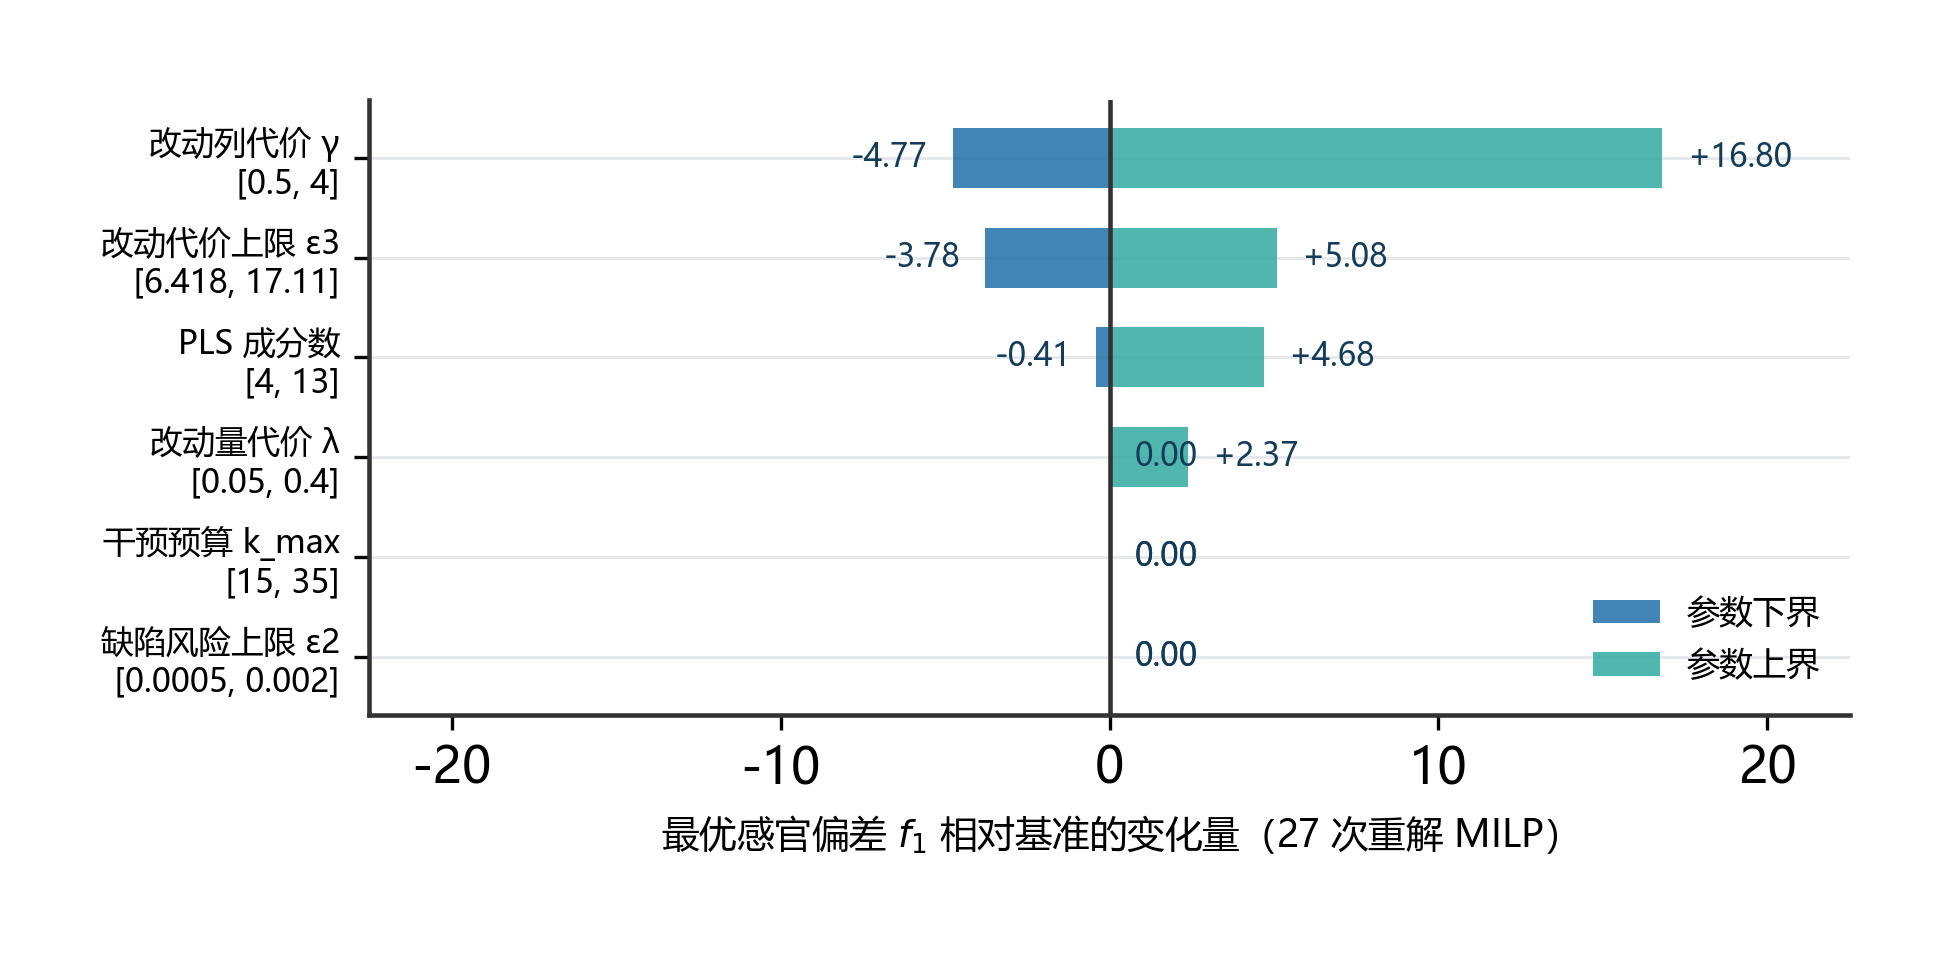
\includegraphics[width=0.79\textwidth]{figures/fig_q3_tornado.png}
\caption{灵敏度分析：27 次重解得到的 $f_1$ 变化量，$\gamma$ 与代理成分数是主导项}
\label{fig:q3tornado}
\end{figure}

三条结论。第一，改动列代价 $\gamma$ 是主导项，摆幅 13.3438，远大于其余各项。$\gamma$ 增大使同一 $\varepsilon_3$ 预算下可改的列数从 10 降到 1,$f_1$ 从 11.080 升到 24.424。这说明“愿意改几个化合物”对结果的影响大于任何数值细节，本文因此把改动数作为显式约束。

第二，代理成分数是第二敏感项，摆幅 9.2310，且不单调：取 4 个成分时 $f_1=25.675$(拟合不足),6 个时降到 20.244,8 个为 20.576，增加到 13 个反而升到 29.475。摆幅超过 9 意味着代理的复杂度设定本身就能让前沿移动三成以上，这是本文坚持“只按段报告、不报单点最优”的量化依据。

第三，缺陷容忍 $\varepsilon_2$ 与干预预算 $k_{\max}$ 的摆幅均为 0，在本例中都是不活跃约束。$\varepsilon_2$ 不活跃是因为双乙酰已被硬约束压到阈值以下，此时 $f_2=0$，放宽上限自然无影响——这正是单位修正后的结果，修正前 $f_2$ 被伪约束固定，扰动 $\varepsilon_2$ 会看似敏感。$k_{\max}$ 不活跃是因为最优解只需改 6 个化合物，上限从 15 放宽到 35 都不变。两点都须写明，否则容易把 $k_{\max}=25$ 误当作结论的驱动因素。

%==============================================================================
% 九、模型评价与推广
%==============================================================================
\section{模型评价与推广}

\subsection{模型优点}

第一，数据核验做得细。本文把题面与实测的六处差异，包括样本数、sheet 数、相关系数类型、交叉矩阵规模、五个理化列的量纲与标签尺度逐条核对并列表，交叉校验达到 $10^{-17}$ 量级，因此后续结论建立在可复核的数据之上，而不是建立在题面文字的转述之上。

第二，三问共用一条证据链。问题一的预测器不只用于报精度，它的失效诊断，即地板效应占比与 $R^2$ 的单调关系解释了问题二为什么有一半记录做不了化学判断；问题二的 Top-3 并集直接构成问题三的 75 维决策空间；问题三的代理又沿用同一套感官定义。三问的结论因此可以互相对照，不会出现各训一个模型、彼此矛盾的情况。

第三，结论都标了可信范围。问题一报区间而非点估计，问题二把一半的 Top-3 记录标为无法做化学判断，问题三以“代理误差大于前沿点间距”为由拒绝给出单点最优。这些否定性结论不是退让，而是本题样本量下的正确表述。

第四，精确解优先。问题三用混合整数线性规划求得的前沿支配了 92.17\% 的 NSGA-II 点、反向支配为 0，且精确解的非支配性逐点验证通过，说明在可以线性化的结构上不应退而用启发式算法。但超体积的对比要谨慎：精确侧只有 7 个点、启发式侧 115 个点，而超体积随点数增加而增大，因此 757.78 对 299.12 不能读成"优 2.5 倍"；真正可比的是支配率与逐点水平。

\subsection{模型不足}

第一，标签不能精确还原。附件4 的连续强度与 0--6 整数分之间不存在可复现的对应关系，本文只能给出近似的分位映射。实测每列最高频取值仅占 1.8\%、等于列最小值仅占 0.88\%，说明标签已被中心化并加过扰动，连“大量样品取最低档”这一结构都无法从数据直接验证——等级比例只能取自感官评价文献而非拟合。即使如此，精确同档率中位也只有 0.376，且附件4 没有整数真值，任何 kappa 都只是映射内的往返一致性，不能称为对面板真值的精度。

第二，问题一的精度与文献持平，但分布高度右偏。均值 0.2223 与文献\cite{schreurs2024}报告的 0.21（梯度提升）、0.22（最优树模型）相当，而本文用的是嵌套交叉验证、选型不进评估折，同等数值下口径更保守。但中位只有 0.1469，比均值低 0.0754：50 项中仅 6 项 $R^2>0.5$（酸度 0.7149、酒精 0.7108、乳酸 0.6768、乙酸 0.6326、苦味 0.5862、酒体 0.5328），有 19 项低于 0.10。按类别拆分，15 个嗅觉项均值 0.1490、中位 0.1194，其余 35 个味觉与口感项均值 0.2536。文献只报一个整体均值，看不出这一分裂；本文并列中位与均值，正是为了把“近半数感官项无法由化学谱解释”显式化。整体喜好项的 $R^2$ 仅 0.1098，仍属最难预测的一类。此外 50 项中只有 7 项的残差通过正态性检验，多数维度的误差结构并非同方差，限制了区间估计的适用面。

第三，问题二的归因不稳定。跨模型 Jaccard 中位仅 0.0974、最小 0.0175、最大也只有 0.2533，说明 Top-3 名单高度依赖模型族；150 条记录中 83 条因阈值表缺项无法做 OAV 检验。因此本文只能报告 19 条双条件交集，这不足以支撑一份完整的“关键化合物清单”。

第四，问题三未经实验验证。代理的逐项 $R^2$ 中位 0.1386、最大误差 3.1525，折合标准差 2.64 倍，且优化中不含化合物间的协同与拮抗，生成的化学谱只是配方调整的方向性候选，不能替代中试与感官评价。另外，五类缺陷物的约束在本文数据下全部退化为 $x_j\leq x^0_j$，敏感性分析显示去掉它们后没有一类会恶化、$f_1$ 代价为 0，即这组约束在本例中不活跃，只能防止更大改动幅度下的触碰；而 trans-2-壬烯醛的阈值只能引用文献，其单位按附件8 标为 mg/L，与样本取值范围不匹配，使该缺陷物只能保证“不恶化”而非“不超标”。

\subsection{模型推广}

本文的做法对同类“高维成分数据 + 主观感官标签 + 小样本”的问题有可迁移性。可迁移的是四个环节：一是用官方对照表核对对数变换与缺失机制，避免自行推断；二是用嵌套交叉验证把模型选择与评估分开，这是小样本下报告 $R^2$ 的诚实做法；三是在强共线下用重采样的入选频率稳定化逐列置换，阈值由稳定选择的界反解；四是用 $\varepsilon$-约束的混合整数线性规划求解多目标，再以启发式算法作对照。这套流程可直接用于食品、香料、烟草等风味体系的成分—感官建模，也可用于药物辅料配比一类的多目标配方设计。

深度条件生成模型在本文场景下未被采用，原因见第八章：样本量不足会使生成器退化为插值器。若数据规模扩大到每风格数百样本，可把收缩高斯换成条件变分自编码器，优化部分仍保留现有的混合整数线性规划结构。

%==============================================================================
% 十、结论
%==============================================================================
\section{结论}

本文围绕商用啤酒风味代谢数据，依次完成感官评分预测、关键化合物归因与受约束的风味指纹重构三项任务，三问共用同一套数据核验与评估标准。

问题一以 231 维化学谱预测 50 个感官项，用外层 5 折、内层 5 折的嵌套交叉验证在岭回归、弹性网、LightGBM 与 ExtraTrees 四个模型间逐项选型。$R^2$ 中位 0.1469、均值 0.2223，49 项为正，可预测性最高的是酸度 0.7149 与酒精感 0.7108。0--6 分级由分位映射给出，加权 kappa 中位 0.3400、34 项超过 0.3；四组等级比例下 kappa 极差为 0.041，而“平移后直接取整”会使 53.2\% 的样本压到 0 分、kappa 跌至 0.1244。结论是分级映射不是收尾步骤，而是问题一能否成立的前提。

问题二先诊断附件2 的化合物网络：原谱聚类因为随机初始化退化为单模块（占 79\% 的节点），改用归一化拉普拉斯后模块度仍接近 0，而 Louvain 算得 $Q=0.3229$、高于度保持零分布的 95\% 分位，说明社区结构真实存在但与化学来源几乎无关（ARI 仅 0.0838），故归因以逐列置换重要性完成，化学族标签只用于解释。200 次自助重采样的入选频率用作稳定性度量，阈值由稳定选择的界反解为 0.5022，属操作性门槛。150 条 Top-3 记录中 19 条 OAV$>1$，其中同时越过筛选阈值的 10 条构成最强证据；另有 8 条接近阈值、40 条浓度远低于阈值、83 条因阈值缺项无法判断。跨模型 Jaccard 中位仅 0.0974，是本文必须如实披露的短板。

问题三以收缩高斯描述 22 个风格的可行域，最近邻距离比 1.076 说明生成没有退化为复制；用 8 成分偏最小二乘作 50 维感官代理，按问题二的 Top-3 并集与三个缺陷物把决策维压到 75，以 DMS、4VG 为硬约束求解 $\varepsilon$-约束的混合整数线性规划，300 个网格点全部可行、去重后得 7 个 Pareto 点。代理目标由基线 48.9620 降至 20.2063（降 58.7\%），前沿从改动 1 个化合物到 10 个连续可调；与手写 NSGA-II 的 115 个非支配点相比，精确前沿支配其中 92.17\%、反向支配为 0。低 $f_1$ 端的解依赖若干降到检出限的极端改动，若按每列 $\pm1$ 个 $\log_{10}$ 单位收紧可行域，降幅会明显收窄。跨风格迁移把偏差从起点 47.1450 降到 13.1366（降 72.14\%），改动了 25 个化合物，五类缺陷物全部不恶化。

三问之间不是并列关系。问题一给出“哪些感官项可预测、哪些不可”的分层判断，这个判断决定了问题二只能交付 19 条双条件交集而不是完整的 50×3 清单；问题二的 Top-3 并集又直接构成问题三的 75 维决策空间，也决定了问题三里哪些感官项能调、哪些只能被动接受。把这条链拆开各做一套，会得到三份互不相容的结论。

可以推广的三条经验：数据先拿官方对照表核一遍，不能照题面文字做；小样本下嵌套交叉验证不能省，否则报出的精度是挑出来的；结论要标可信范围，宁可否定自己的一部分结果，也不要给经不起追问的单一答案。


\newpage
\referencescn

\newpage
%==============================================================================
% 十一、AI 工具使用声明（按官方规定置于参考文献之后）
%==============================================================================
\phantomsection
\section*{AI 工具使用声明}
\addcontentsline{toc}{section}{AI 工具使用声明}

按照竞赛关于人工智能工具使用的规定，本文声明如下。

所用工具：Hermes Agent（Nous Research），底层模型 deepseek-v4-flash（深度求索 DeepSeek），使用日期 2026 年 10 月\cite{deepseek}。工具与模型分属两家机构，此处分列以免混淆。

使用环节：代码编写与调试、图表绘制脚本的整理、文稿的文字润色。

未使用 AI 的环节：选题判断、建模思路与模型选型的确定、评价指标的选取、数据核验结论的判断、结果的取舍与结论提炼，均由参赛队员独立完成。

AI 生成内容的人工核验与修正：参赛队员对全部数值与结论逐条复核，发现并修正了以下问题。其一，初版把附件4 的连续强度直接当有序类别处理，且对预测与真值各做一次分位映射，导致加权 kappa 虚高；现改为只对真值定切点、预测沿用同一映射。其二，初版漏掉了附件8 感官名称表中 24 个感官项被标注为分类变量这一事实，现已按连续强度统一处理并在正文说明依据。其三，问题三初版把缺陷物阈值一律取 $\log_{10}$，使处于线性量纲域的双乙酰软约束退化为常数、$f_2$ 被固定在 0.524；现已逐列判断量纲域并修正，$f_2$ 可以真正降到 0。其四，初版引用的重采样次数与代码不符，现按实际运行结果改为问题一 1000 次、问题二 200 次。上述修正过程与结果均记录在支撑材料中，可复现。

参赛队对本文引用 AI 工具生成内容的正确性、可靠性与学术规范性负责。


\newpage
\appendixcn

\end{document}
